\documentclass{article}
\usepackage{titling}
\usepackage{graphicx}
\usepackage{caption}
\usepackage{subcaption}
\graphicspath{{graphics/}{../traffic_data_analysis/traffic_data_analysis/plots/}}

\pretitle{
  \begin{center}
  \huge
  
\includegraphics[width=10cm]{graphics/PSU_logo_transparent.png}\\[\bigskipamount]
}
\posttitle{\end{center}}
\usepackage{unicode-math}
\usepackage{amsfonts}
\usepackage{booktabs}
\usepackage{longtable}
\usepackage{array}
\usepackage{multirow}
\usepackage{wrapfig}
\usepackage{float}
\usepackage{colortbl}
\usepackage{pdflscape}
\usepackage{tabu}
\usepackage{threeparttable}
\usepackage{xcolor}
\usepackage{soul}
\usepackage{fancyhdr}
\usepackage{hyperref}
\usepackage{float}
\pagestyle{fancy}
\rhead{
\includegraphics[width = .05\textwidth]{graphics/psulogo2.jpg}}
\usepackage{geometry}
\geometry{a4paper, margin=0.75in}

\title{Portland Traffic Analysis: Final Report}
\author{
  Xu, Suru\\
  \texttt{suru@pdx.edu}
  \and
  Nelson, Austen\\
  \texttt{ajn6@pdx.edu}
}

\date{\today}

\begin{document}

\maketitle

\tableofcontents

\section{Executive Summary}

The COVID-19 pandemic significantly altered traffic patterns in Portland, reshaping commuter behavior and roadway demand. This report analyzes historical traffic count data to assess how peak traffic periods and overall volumes have shifted on two major highway crossings: the I-5 and Glenn Jackson bridges.

Our analysis identifies key changes in traffic demand across different time periods and weekdays, highlighting how commuter habits have evolved post-pandemic. Findings indicate a notable flattening of morning rush-hour peaks, a slight reduction in afternoon traffic volumes, and relatively stable weekend travel patterns. Additionally, distinct variations between the two bridges suggest localized differences in travel behavior and infrastructure utilization.

These insights provide valuable guidance for transportation planning, congestion management, and infrastructure investments. As commuting patterns continue to adapt, future studies incorporating real-time data sources could further refine our understanding of long-term traffic trends in the region.

\section{Introduction and Background}
The COVID-19 pandemic brought significant shifts in mobility patterns, altering daily commutes and reshaping traffic flow on major highways \cite{covid_mobility_emissions, traffic_hiatus_covid}. This study investigates these changes by analyzing historical traffic count data, with a focus on two critical transportation corridors in the Portland area: the I-5 and Glenn Jackson bridges. Understanding how traffic demand and peak periods have evolved post-pandemic is essential for transportation planning, congestion management, and infrastructure development. These insights can inform policy decisions on commuting patterns, public transit investments, and roadway capacity planning.

To address these needs, the Oregon Department of Transportation (ODOT) seeks a comprehensive, data-driven analysis using historical traffic data from Automatic Traffic Recorders (ATR). To capture the impact of the pandemic on traffic behavior, this report explores the following key questions:

\begin{itemize}
    \item How have peak traffic periods changed in terms of structure (flatter, sharper, later, or earlier throughout the day) at these key locations?
    \item How has daily traffic demand shifted across different days of the week at these bridges?
    \item Are there distinct trends between these two major highway crossings?
\end{itemize}

\section{Data}

ATR data provides 24/7 traffic volume at specific highway locations across Oregon and has been curated by ODOT’s monitoring unit for high reliability. The data consists of vehicle counts over hourly time periods at 12 different highway locations, each consisting of 2 opposite directions (either NB/SB or EB/WB). Some locations have many more years available than others, but in total there are about 3.25 million hours of data recorded over the 24 location and direction combinations.

Preliminary analysis of median values reveals notable trends and location-specific patterns in the data. Table \ref{tab:medians} presents an approximation to weekday peak-time and peak-volume based on cubic periodic spline interpolation of hourly medians. 

General visible trends seem to be a slightly later peak traffic time in the mornings and location dependent changes in afternoon peak times. The peak volume is lower post-Covid all across the board, with very few exceptions outside of data availability issues. 

\subsection{Data Quality}
Overall, the provided dataset is high quality and quite complete. For a visual representation of the time coverage for each location / direction combination, see figure \ref{fig:data_availability}. The only issues with data quality we discovered in our analysis fall into two main categories:

\begin{enumerate}
    \item Daylight Savings (DST) Inconsistencies 

        The dataset is recorded in Coordinated Universal Time (UTC), which does not account for Daylight Savings Time (DST) adjustments. This led to occasional timestamp misalignments, particularly at midnight during the spring transitions (April before 2006 and March in later years). These discrepancies suggest that some timestamps may have been incorrectly converted or recorded, potentially affecting time-sensitive traffic analyses. A visual example where this happens is shown in figure \ref{fig:dst_example}, where counts from March through August are clearly shifted exactly one hour forward during the early morning hours when the traffic is most consistent. 

        While these inconsistencies do not significantly impact most analyses, they can introduce errors in identifying precise peak-hour shifts. In particular, Table \ref{tab:medians} shows instances where peak times appear to shift by nearly an hour (e.g., Vista Ridge EB 2018, Wilsonville SB 2024, and Interstate Bridge NB 2024). Further adjustments to correct for these errors may be beneficial for future studies.

    \item Under-Reported and Malformed Data

        Sensor malfunctions and estimation techniques introduced inconsistencies in some data points, as noted in the reliability report provided by the client. Certain locations and time periods exhibited artificially low traffic volumes due to under-reporting or data imputation. One example of this problematic data is I5 bridge SB for the year 2018. During this time there was a construction project so traffic could potentially be lower, but reported (potentially estimated) values are so low that the period is not useful for analysis.

        Another example of malformed data is periods of time with many zero values. In the reliability report it is stated that the 2024 Vista Ridge Tunnel data is reliable, but from 10-07 to 12-23 there are 1440 hourly entries with 0 and 1872 non-zero hourly entries.

        To enhance data reliability, future datasets could incorporate an additional column flagging estimated or low-confidence entries. This would allow for selective filtering, ensuring that models account for data reliability and providing transparency in trend analysis.
\end{enumerate}

A complete listing of potential issues we found in the analysis can be found in appendix \ref{app:data_issues}. 

\section{Methods}

\subsection{Generalized Additive Model (GAM)}

Generalized Additive Models (GAMs) are an extension of generalized linear models that allow for flexible modeling of non-linear relationships by representing the target variable as an additive combination of smooth functions of the explanatory variables \cite{gam, gam_truck_drivers, gam_crash_frequency}. This flexibility makes GAMs particularly suitable for capturing complex patterns in data without imposing strict parametric forms.

In our analysis, we focus on modeling hourly traffic counts (\( y \)) as a function of variables such as the hour of the day (\( h \)), month of the year (\( m \)), and a binary indicator for the period relative to the COVID-19 pandemic (\( p \)), where \( p = 0 \) denotes pre-pandemic and \( p = 1 \) denotes post-pandemic periods. The GAM framework allows us to express this relationship as:

\[
y = s_1(h) + s_2(ph) + s_3(m) + \epsilon
\]

Here, \( s_1 \), \( s_2 \), and \( s_3 \) are smooth functions estimated from the data, and \( \epsilon \) represents the error term. The inclusion of the interaction term \( ph \) enables the model to capture differential effects of the pandemic across different hours of the day.

A key advantage of GAMs is their interpretability; the additive components \( s_i \) provide insights into how each explanatory variable individually influences the target variable. To estimate these smooth functions, we employ spline functions, which are piecewise polynomials joined smoothly at specific points known as knots. Splines offer greater flexibility than global polynomials and help mitigate issues such as the Runge phenomenon—a problem where high-degree polynomial interpolation can lead to large oscillations at the boundaries of the interpolation interval (classic German reference: \cite{runge1901empirische}).

For implementation, we utilize the \texttt{scikit-learn} library's tools for spline fitting. The library provides functionalities to construct spline basis functions and integrate them into a regression framework, facilitating the estimation of the smooth components in the GAM \cite{scikit-learn}. This approach allows us to model the non-linear relationships in the traffic data effectively while maintaining computational efficiency and interpretability.

After some experimentation we found the periodic cubic splines with knot positions:
\begin{itemize}
    \item 15 uniform knots for $s_1$ 
    \item knots located at $(0, 4, 6, 8, 10, 15, 17, 19, 24)$ for $s_2$
    \item 4 uniform knots for $s_3$ 
\end{itemize}
generalized well for our data. The knots for $s_3$ were chosen because we are primarily interested in the effect on peak traffic periods, so we choose the knots to be more densely located during these times to give the model more ability to express differences in the interaction while limiting negative effects of over-paramaterizing the model.

\subsection{Maximum Mean Discrepancy (MMD)}

Traditional statistical methods often rely on parametric assumptions, which may fail to capture the complexity and high-dimensional nature of real-world traffic patterns. To address these limitations, Maximum Mean Discrepancy provides a robust, non-parametric alternative for detecting shifts in traffic distributions.
MMD is a kernel-based statistical test that quantifies differences between probability distributions without imposing parametric constraints. By embedding distributions in a reproducing kernel Hilbert space (RKHS), MMD enables a flexible two-sample comparison by mapping traffic data into a high-dimensional space and evaluating the divergence in their mean embeddings. This approach is particularly well-suited for assessing shifts in traffic patterns before and after the pandemic, offering a data-driven framework for capturing complex, non-linear changes in distribution.

\subsubsection{Data Structuring Strategy}

To ensure a systematic comparison of pre- and post-pandemic traffic patterns, the dataset is structured into two key dimensions:
\begin{enumerate}
    \item Time segmentation through monthly groups
    \item Traffic behavior segmentation by day-type classification
\end{enumerate}

This structure allows for temporal consistency and prevents confounding effects from seasonal or weekday variations.

\paragraph{Monthly Grouping for Temporal Consistency}

To account for variation in traffic demand across different times of the year, we divide the dataset into five distinct monthly groups instead of using traditional seasonal definitions. This prevents seasonal confounders from affecting our analysis.

\begin{itemize}
    \item \textbf{January–February:} Typically, the lowest traffic counts due to winter weather conditions.
    \item \textbf{March:} Contains Spring break week, influencing travel demand.
    \item \textbf{April–May \& September–October:} Stable school/work schedules, making them strong baseline months for comparison.
    \item \textbf{June–July–August:} Summer months with a different traffic pattern, characterized by fewer school-related trips and more recreational travel.
    \item \textbf{November–December:} Affected by winter conditions and holiday travel, introducing variability in demand.
\end{itemize}

This grouping strategy ensures that traffic trends are analyzed under similar external conditions before and after the pandemic.

\paragraph{Day-Type Classification for Behavioral Segmentation}

Traffic patterns vary based on the day of the week, requiring further classification to capture meaningful behavioral trends. We categorize traffic data into four primary day types:

\begin{itemize}
    \item \textbf{Monday \& Friday:} Often show distinct travel behaviors, with Friday frequently exhibiting early departures and heavier congestion.
    \item \textbf{Tuesday–Wednesday–Thursday (T/W/T):} Assumed to have relatively consistent traffic patterns, grouped together for statistical efficiency.
    \item \textbf{Saturday \& Sunday (Weekends):} Typically show non-commuting, recreational travel behaviors, distinct from weekday traffic trends.
\end{itemize}

By applying this dual-layered structuring approach, we ensure that comparisons between pre- and post-pandemic traffic data are made under logically consistent conditions, minimizing external sources of variation.

\subsubsection{MMD Model for Traffic Pattern Comparison}

After structuring the dataset, we use the Maximum Mean Discrepancy statistic to measure shifts in traffic distributions. Given two sets of traffic data:

\[
X = \{x_{i,j} \mid i = 1, \dots, N; j = 1, \dots, 24\}, \quad Y = \{y_{i,j} \mid i = 1, \dots, M; j = 1, \dots, 24\}
\]

where:

\begin{itemize}
    \item $x_{i,j}$ and $y_{i,j}$ are traffic counts at hour $j$ on day $i$ for pre- and post-pandemic periods, respectively.
    \item $X$ and $Y$ represent hourly traffic counts for each day type within a specific monthly group.
\end{itemize}

As shown in \citet{Gretton2019}, the MMD statistic is calculated as:

\[
\text{MMD}^2(X, Y) = \mathbb{E}_{x,x'}[k(x, x')] + \mathbb{E}_{y,y'}[k(y, y')] - 2\mathbb{E}_{x,y}[k(x, y)]
\]

where \( k(\cdot, \cdot) \) is a kernel function. This provides a non-parametric measure of distributional shift in traffic behavior.

\subsubsection{Statistical Inference Using Permutation Testing}

Statistical significance is evaluated using a permutation test. Traffic data is pooled and randomly reassigned into new pre- and post-pandemic groups, maintaining the same sample sizes as the original datasets. The MMD statistic is then recomputed for each permutation, generating an empirical distribution under the null hypothesis. The p-value is estimated as the proportion of permuted MMD values that exceed or equal the observed MMD, ensuring statistical robustness in assessing distributional differences.

The empirical p-value is calculated as:

\[
    p = \frac{\sum_{b=1}^{B} \boldsymbol{\mathbb{1}}(\text{MMD}^2_b \geq \text{MMD}^2_{\text{obs}})}{B}
\]

where \( B \) is the number of permutations, \( \text{MMD}^2_{\text{obs}} \) is the observed MMD statistic, and \( \mathbb{1}(\cdot) \) is an indicator function \cite{Gretton2012}.

This methodology allows us to determine whether the observed shift in traffic patterns is statistically significant or could have arisen due to random fluctuations.

\section{Results}

\subsection{Generalized Additive Model}

Visualizations of the GAMs for each ATR location are found in the appendix in section \ref{sec:gam_figs}. The primary findings can be classified into three main categories:

\subsubsection{Weekday `Morning Rush'}

Examples of ATR locations with strong weekday `morning rush' characteristics (usually heading into the metro area) are Vista Ridge Tunnel EB, Interstate Bridges SB, and Iowa Street NB. The general visible change in the morning rush at these locations is a reduction in peak volume and often a slight shift to later in the day. This reduction in peak volume is seen as a `flatter' morning peak where the most intense traffic in the morning is spread out over a longer period of time. A clear outlier to these patterns is Wilsonville NB which has almost identical morning traffic patterns. 

The observed reduction in morning peak volume could be attributed to decreased demand, increased congestion, or a combination of both; however, this dataset alone does not allow for a definitive conclusion. Only for some locations is this reduction compensated by increases in volume later throughout the mid-day.

\subsubsection{Weekday `Afternoon Rush'}

ATR locations with `afternoon rush' characteristics are often the directional pairs to those with `morning rush' ones. The afternoon rush structure is much different, generally less concentrated and spread out over a longer period. The changes in afternoon traffic are less pronounced than the morning ones and the peak volume times are mostly consistent before and after Covid-19. The most obvious change is a slight earlier shift in when the traffic volume begins to taper off and a slight reduction in peak volume counts.

\subsubsection{Weekend}

The visible changes in weekend patterns is much less pronounced than the weekday ones, which is confirmed quantitatively with the statistically testing using MMD discussed in section \ref{sec:mmd_results}. Although less pronounced, there is still a visible reduction in volume at most locations. 

\subsection{Maximum Mean Discrepancy} \label{sec:mmd_results}

To evaluate the statistical significance of traffic pattern shifts, we applied the Maximum Mean Discrepancy test along with a permutation test. The results are visualized in heatmaps, where each cell represents the p-value associated with traffic distribution changes for a specific combination of day type and month group.

\subsubsection{Key Observations and Implications}

The findings indicate that the most notable adjustments in traffic patterns occur midweek (Tuesday–Thursday), where consistent shifts are observed across multiple month groups. Mondays and Fridays display a more variable pattern, with changes appearing more context-dependent. Weekend traffic remains relatively stable, with some month-specific variations.

These observations suggest that changes in travel behavior post-pandemic are more evident in structured weekday commuting patterns rather than in discretionary weekend travel. Additionally, differences between I-5 and I-205 may be influenced by location-specific factors such as infrastructure, urbanization, or regional travel demand.

\subsubsection{Summary of Observations}

Based on the analysis, the following key patterns emerge:

\begin{enumerate}
    \item Tuesday–Thursday traffic shows consistent changes across all month groups, suggesting adjustments in midweek commuting behavior.
    \item Monday and Friday display variability in changes, with certain months exhibiting stability and others showing shifts.
    \item Weekend travel remains largely stable, particularly on I-5, while I-205 exhibits some month-dependent variations.
    \item I-5 demonstrates broader consistency in traffic changes, while I-205 presents greater fluctuations across different month groups.
\end{enumerate}

These findings highlight how post-pandemic travel behavior varies across different day types, with midweek commuting experiencing the most pronounced shifts, while weekend travel remains relatively stable.

\section{Conclusions}

This report analyzed traffic patterns on key highway crossings in Portland, focusing on pre- and post-pandemic trends using ATR data. Our investigation employed both Generalized Additive Models (GAM) and Maximum Mean Discrepancy (MMD) testing to capture changes in peak traffic times, overall volume, and distributional shifts across different time periods and day classifications. The following key insights emerged from our study:

\begin{enumerate}
\item \textbf{Morning Rush Flattening:} Peak morning traffic volumes have decreased post-pandemic, often accompanied by a later shift in peak times. This suggests changes in commuter behavior, possibly due to increased telecommuting or flexible work schedules.
\item \textbf{Afternoon Stability:} Unlike the morning rush, the afternoon peak period remains relatively stable in timing and structure. However, a slight reduction in volume is observed, and the peak tapering off occurs earlier in some locations.
\item \textbf{Weekend Traffic Resilience:} Weekend traffic patterns have shown less significant shifts compared to weekdays. Volume reductions are present but less pronounced, indicating that discretionary travel has been less affected by post-pandemic behavioral changes.
\item \textbf{Variability by Location:} While general trends hold across the studied locations, site-specific differences highlight the impact of infrastructure, urban development, and local travel needs. The Interstate Bridge and Glenn Jackson Bridge exhibit distinct post-pandemic traffic shifts, suggesting that regional travel demand and alternate route usage may have evolved.
\item \textbf{Data Quality Considerations:} Our analysis identified some inconsistencies in the ATR dataset, including potential daylight savings time discrepancies and under-reported or estimated data. Addressing these concerns by incorporating reliability indicators in the dataset could improve future modeling efforts.
\end{enumerate}


These findings align with previous studies that have documented significant alterations in urban mobility and emissions during the pandemic \cite{covid_mobility_emissions}. Our findings suggest that long-term shifts in commuting behavior post-pandemic may continue to impact transportation planning. The observed flattening of morning peaks and reduction in overall volume could inform future infrastructure development, congestion management strategies, and transit planning. Further studies incorporating traffic flow models and real-time congestion data could provide deeper insights into the mechanisms driving these changes and their long-term implications for urban mobility.

\subsection{Code Availability}

The code used for analysis and generating this report can all be found in the \href{https://github.com/aujxn/portland_traffic_analysis}{GitHub repo} and is free to use and distribute under the MIT license. 

\bibliographystyle{plain}
\bibliography{references}

\pagebreak

\appendix

\section{Median Peak Time and Volumes}

\definecolor{Gray}{gray}{0.9}
\newcolumntype{g}{>{\columncolor{Gray}}r}
\begin{figure}[H]
\captionof{table}{Weekday Peak Time Table} \label{tab:medians} 
\begin{tabular}{l l *{9}{g}}
    \toprule
    \rowcolor{white}
    \multicolumn{3}{c}{\textbf{Location Info}} & 
    \multicolumn{4}{c}{\textbf{Median Peak Time}} & 
    \multicolumn{4}{c}{\textbf{Median Peak Volume}}\\

    \cmidrule(lr){1-3} \cmidrule(lr){4-7} \cmidrule(lr){8-11}

    \rowcolor{white}
    \textbf{ID} & \textbf{Name} & \textbf{Dir} & 
    \textbf{2018} & \textbf{2019} & \textbf{2023} & \textbf{2024} &
    \textbf{2018} & \textbf{2019} & \textbf{2023} & \textbf{2024}\\ 

    \cmidrule(lr){1-3} \cmidrule(lr){4-7} \cmidrule(lr){8-11}

    \rowcolor{white}\rule{0pt}{4ex}
\multirow{2}{*}{34007} & \multirow{2}{*}{North Plains} &EB & 06:35 & 06:38 & 06:49 & 06:52 & 918 & 939 & 797 & 811 \\
& & WB & 16:06 & 16:03 & 15:49 & 15:55 & 1145 & 1166 & 1121 & 1167 \\
\rowcolor{white}\rule{0pt}{4ex}
\multirow{2}{*}{26022} & \multirow{2}{*}{Lents} &SB & 15:09 & 16:32 & 16:29 & 16:32 & 5521 & 5542 & 5250 & 5187 \\
& & NB & 06:23 & 06:26 & 07:01 & 06:58 & 5055 & 5060 & 5152 & 5111 \\
\rowcolor{white}\rule{0pt}{4ex}
\multirow{2}{*}{26002} & \multirow{2}{*}{Vista Ridge Tunne} &EB & 06:38 & 07:38 & 07:21 & 07:27 & 5047 & 4953 & 4695 & 4602 \\
& & WB & 07:15 & 07:18 & 15:34 & 07:24 & 5623 & 5612 & 5169 & 5173 \\
\rowcolor{white}\rule{0pt}{4ex}
\multirow{2}{*}{26001} & \multirow{2}{*}{Troutdale} &WB & 14:34 & 14:19 & 14:51 & 14:48 & 1229 & 1311 & 1266 & 1294 \\
& & EB & 10:26 & 10:40 & 10:11 & 10:08 & 1286 & 1368 & 1279 & 1331 \\
\rowcolor{white}\rule{0pt}{4ex}
\multirow{2}{*}{26004} & \multirow{2}{*}{Interstate Bridge} &SB & 06:29 & 05:34 & 06:09 & 06:06 & 1908 & 5609 & 5224 & 4939 \\
& & NB & 16:32 & 16:09 & 16:06 & 16:44 & 4619 & 4805 & 4625 & 4380 \\
\rowcolor{white}\rule{0pt}{4ex}
\multirow{2}{*}{26028} & \multirow{2}{*}{Fairview} &EB & 16:29 & 16:35 & 16:18 & 16:29 & 4493 & 4532 & 4391 & 4369 \\
& & WB & 06:29 & 06:35 & 06:41 & 06:35 & 4034 & 4064 & 3850 & 3761 \\
\rowcolor{white}\rule{0pt}{4ex}
\multirow{2}{*}{26024} & \multirow{2}{*}{Glenn Jackson Bridge} &NB & 15:06 & 15:06 & 15:06 & 14:45 & 7168 & 7137 & 6728 & 6614 \\
& & SB & 06:15 & 06:18 & 06:44 & 06:20 & 7411 & 7354 & 6188 & 6159 \\
\rowcolor{white}\rule{0pt}{4ex}
\multirow{2}{*}{34010} & \multirow{2}{*}{Beaverton-Bethany} &EB & 16:03 & 16:03 & 06:49 & 06:49 & 4521 & 4464 & 4191 & 4211 \\
& & WB & 07:15 & 07:15 & 16:21 & 16:24 & 4975 & 5152 & 4500 & 4531 \\
\rowcolor{white}\rule{0pt}{4ex}
\multirow{2}{*}{3011} & \multirow{2}{*}{Wilsonville} &SB & 14:57 & 14:57 & 14:37 & 15:40 & 3778 & 3791 & 3625 & 3640 \\
& & NB & 05:57 & 05:54 & 06:06 & 06:03 & 3832 & 3837 & 3756 & 3871 \\
\rowcolor{white}\rule{0pt}{4ex}
\multirow{2}{*}{26014} & \multirow{2}{*}{Hoyt} &WB & 05:40 & 05:37 & 06:03 & 06:03 & 5850 & 5809 & 5344 & 5363 \\
& & EB & 13:56 & 13:51 & 13:45 & 13:42 & 5587 & 5569 & 5283 & 5247 \\
\rowcolor{white}\rule{0pt}{4ex}
\multirow{2}{*}{3016} & \multirow{2}{*}{Stafford} &NB & 13:59 & 14:05 & 14:05 & 14:05 & 3267 & 3411 & 3186 & 3283 \\
& & SB & 06:23 & 06:23 & 06:55 & 06:55 & 3353 & 3367 & 3222 & 3309 \\
\rowcolor{white}\rule{0pt}{4ex}
\multirow{2}{*}{26016} & \multirow{2}{*}{Iowa Street} &SB & 16:32 & 16:29 & 16:29 & 16:26 & 5374 & 5339 & 4786 & 4758 \\
& & NB & 06:29 & 06:32 & 07:12 & 07:09 & 5687 & 5671 & 5303 & 5231 \\

\end{tabular}\par 
\bigskip 
    Hourly median traffic volume for each entry (location, direction, year) for weekdays is interpolated with a cubic spline to find approximate peak traffic time.
\end{figure}

\section{MMD Groupings}

\begin{figure}[H]
	\centering
	\begin{subfigure}[b]{0.45\textwidth}
		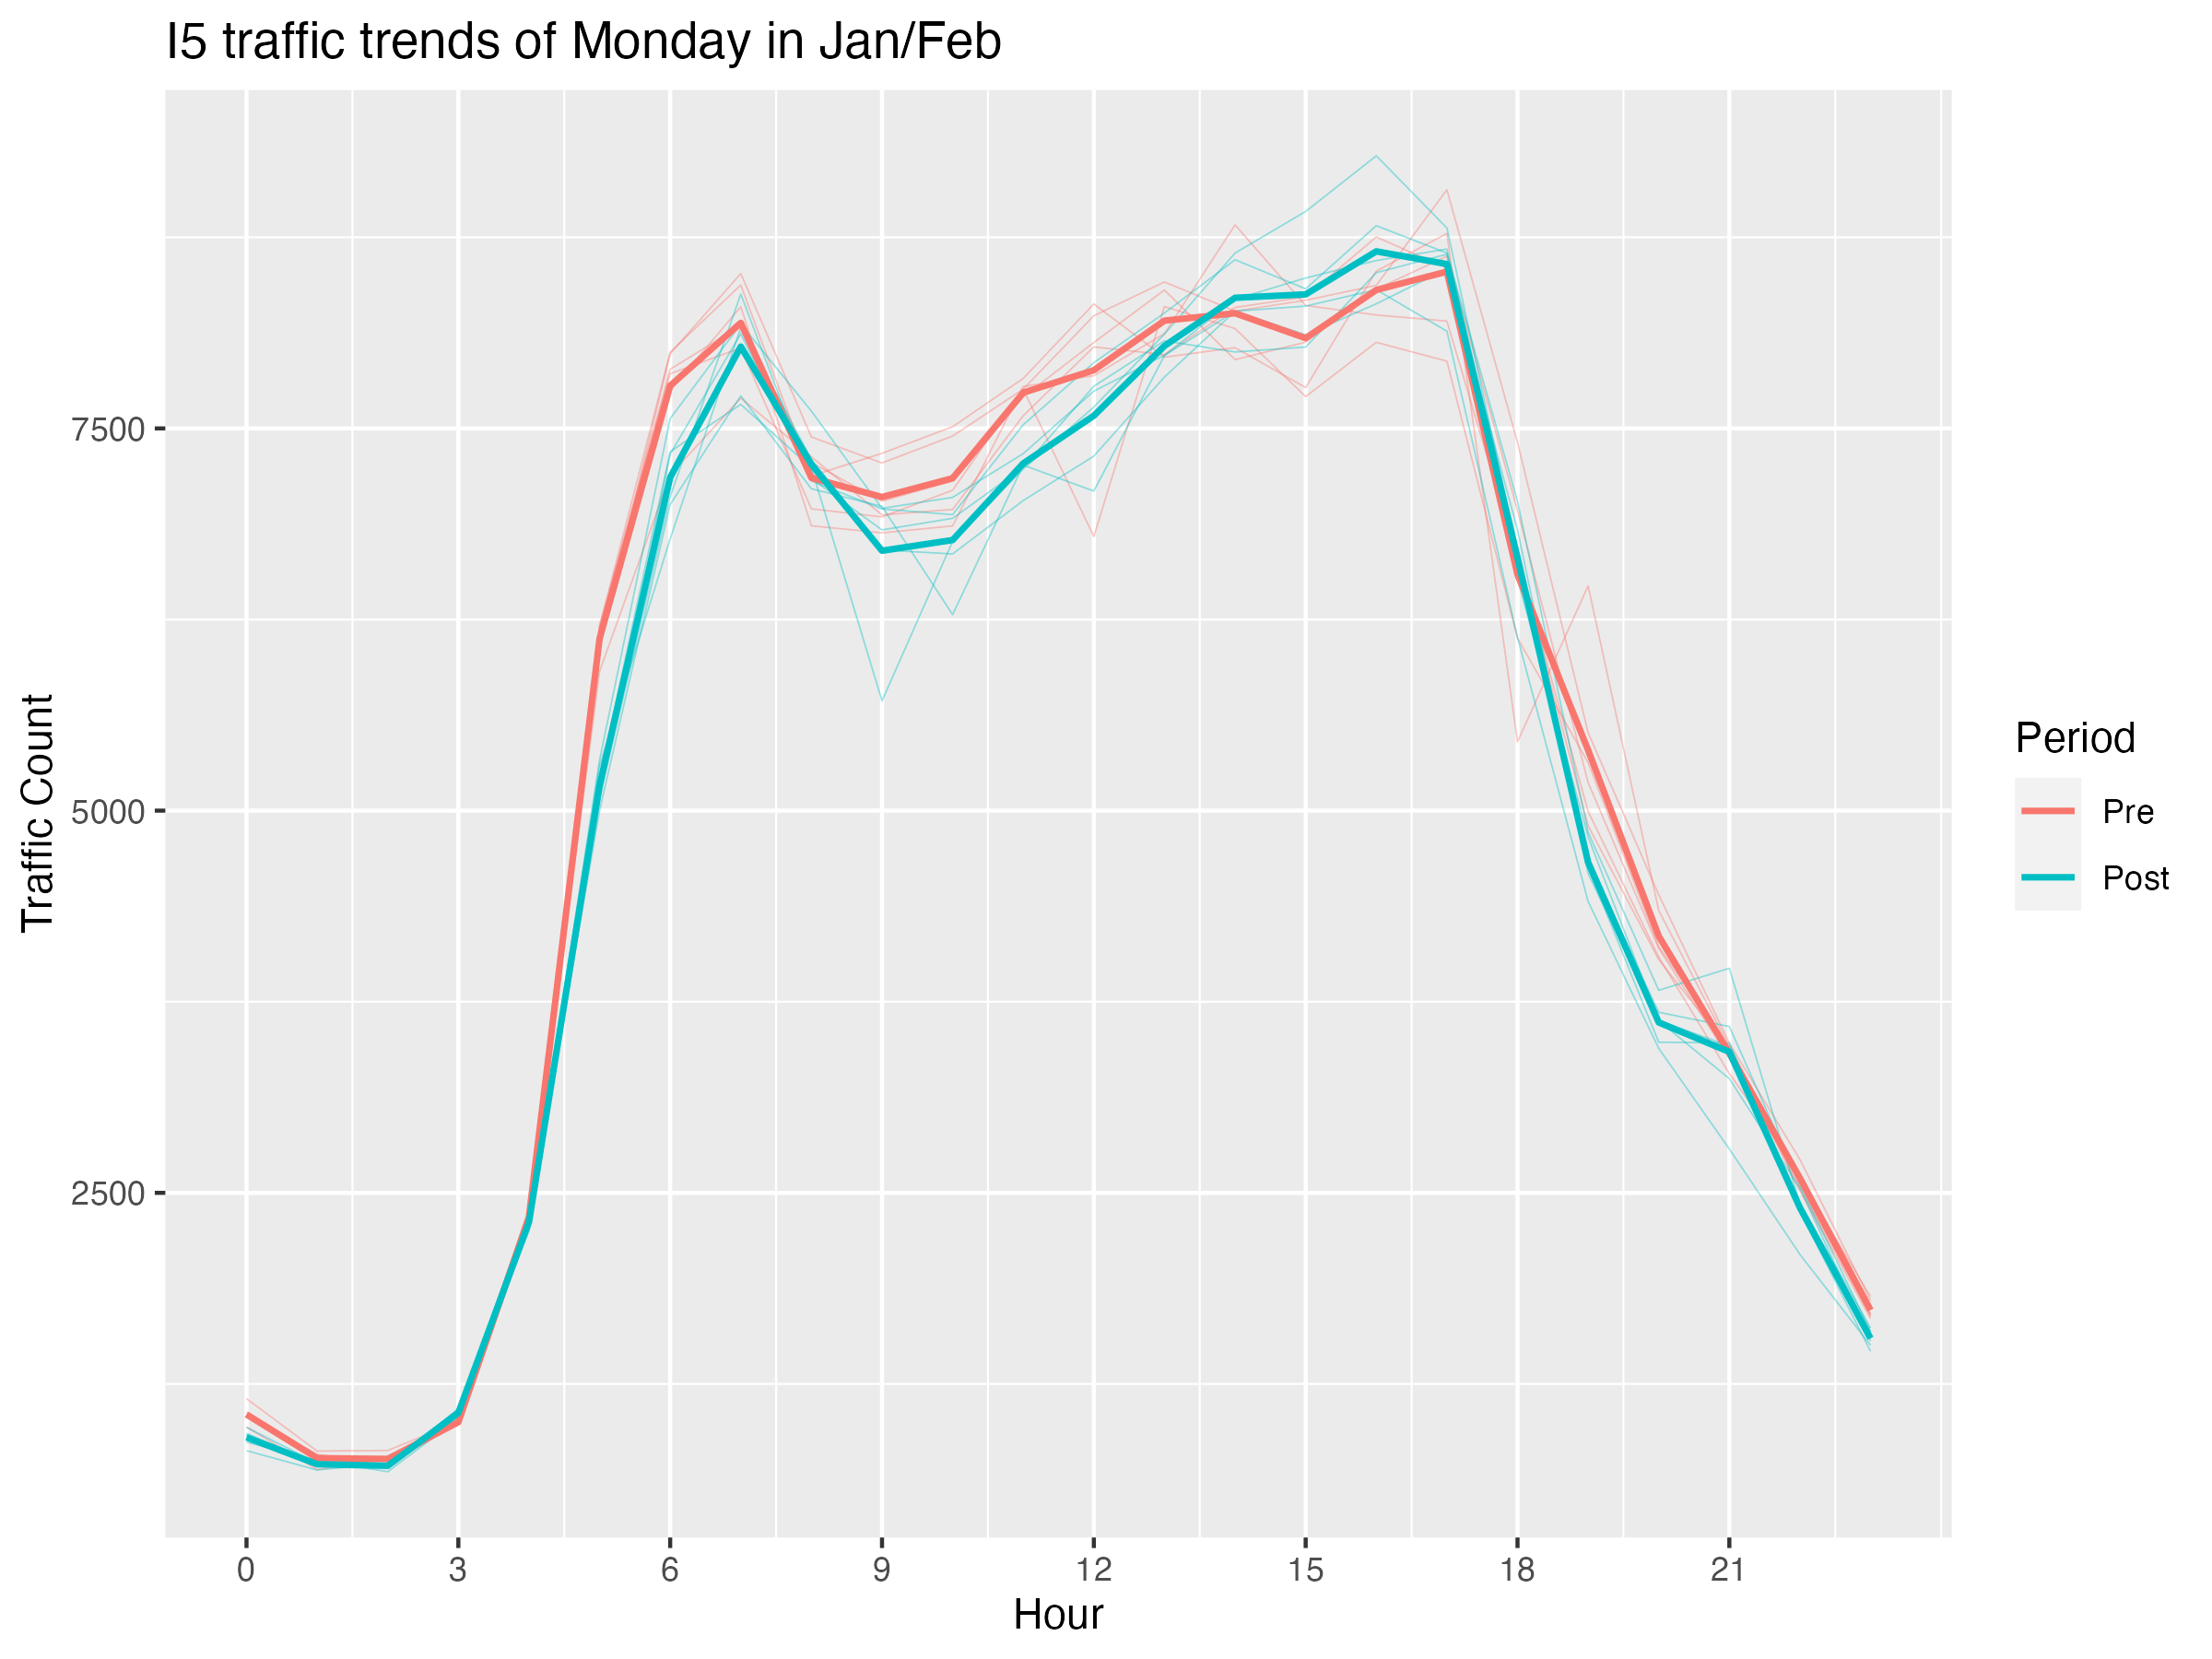
\includegraphics[width=\textwidth]{ATR26004_Plots/picture1_A04.png}
	\end{subfigure}
	\hfill
	\begin{subfigure}[b]{0.45\textwidth}
		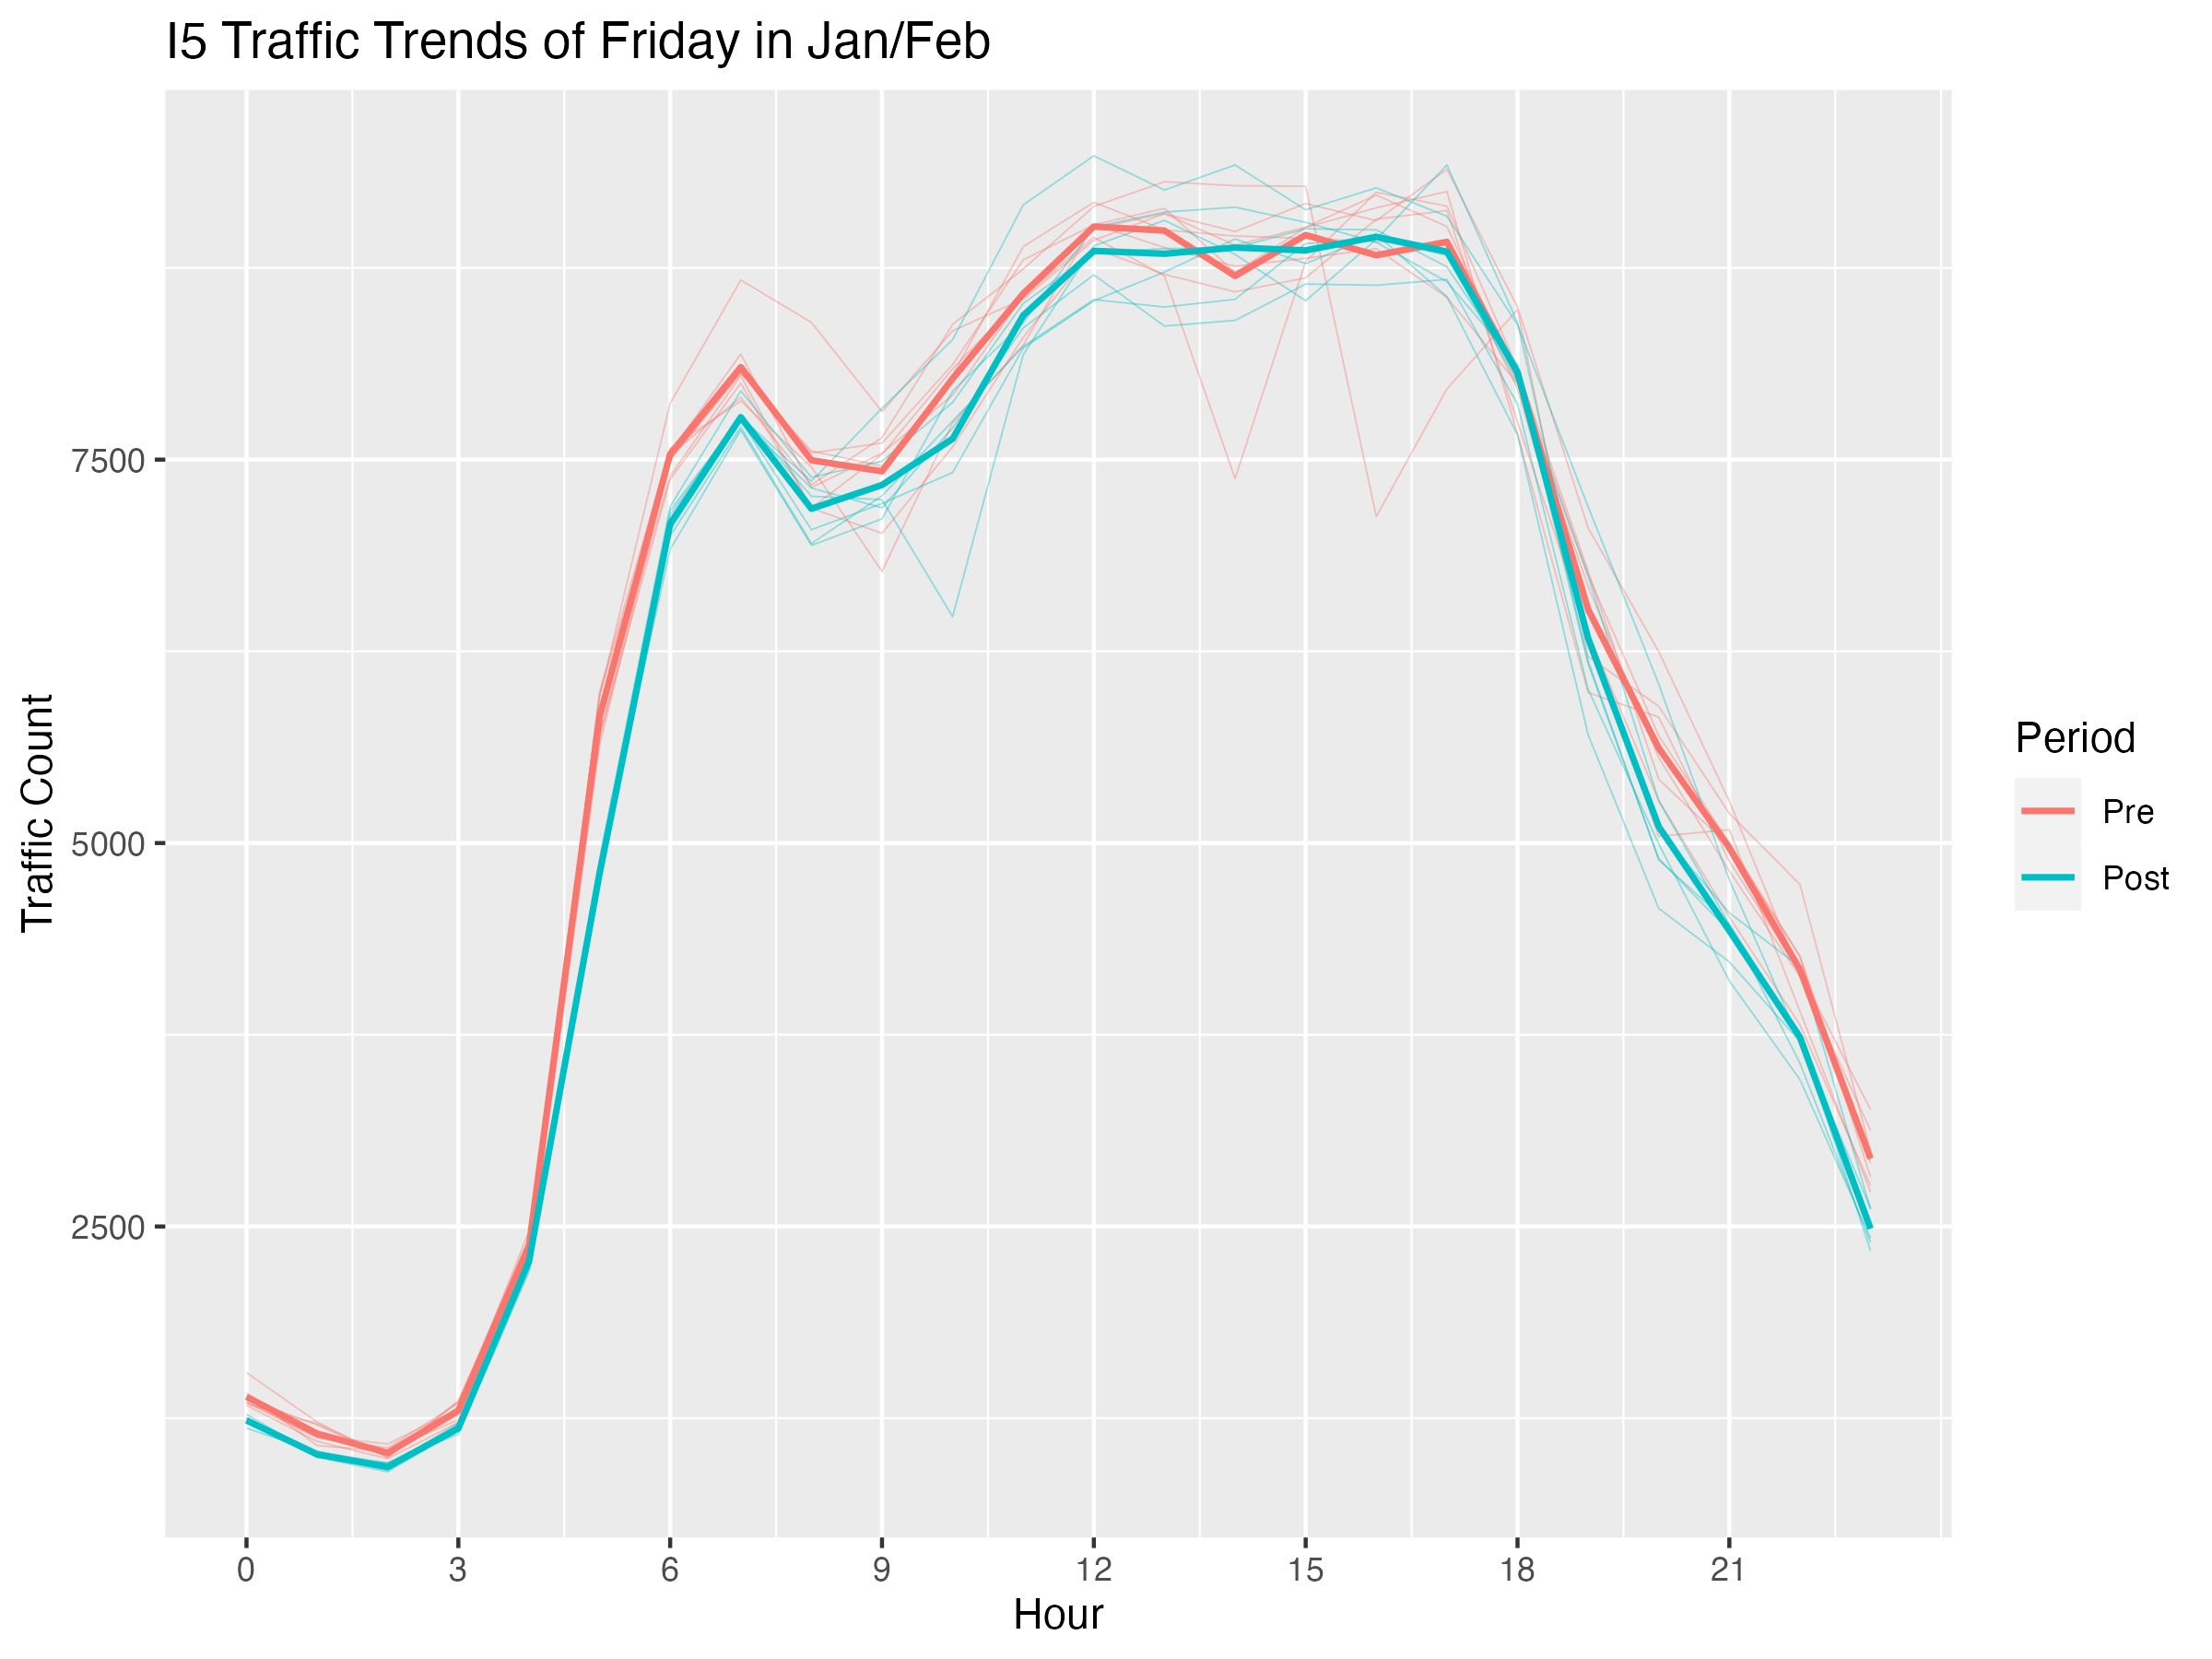
\includegraphics[width=\textwidth]{ATR26004_Plots/picture11_A04.png}
	\end{subfigure}
\end{figure}

\begin{figure}[H]
	\centering
	\begin{subfigure}[b]{0.45\textwidth}
		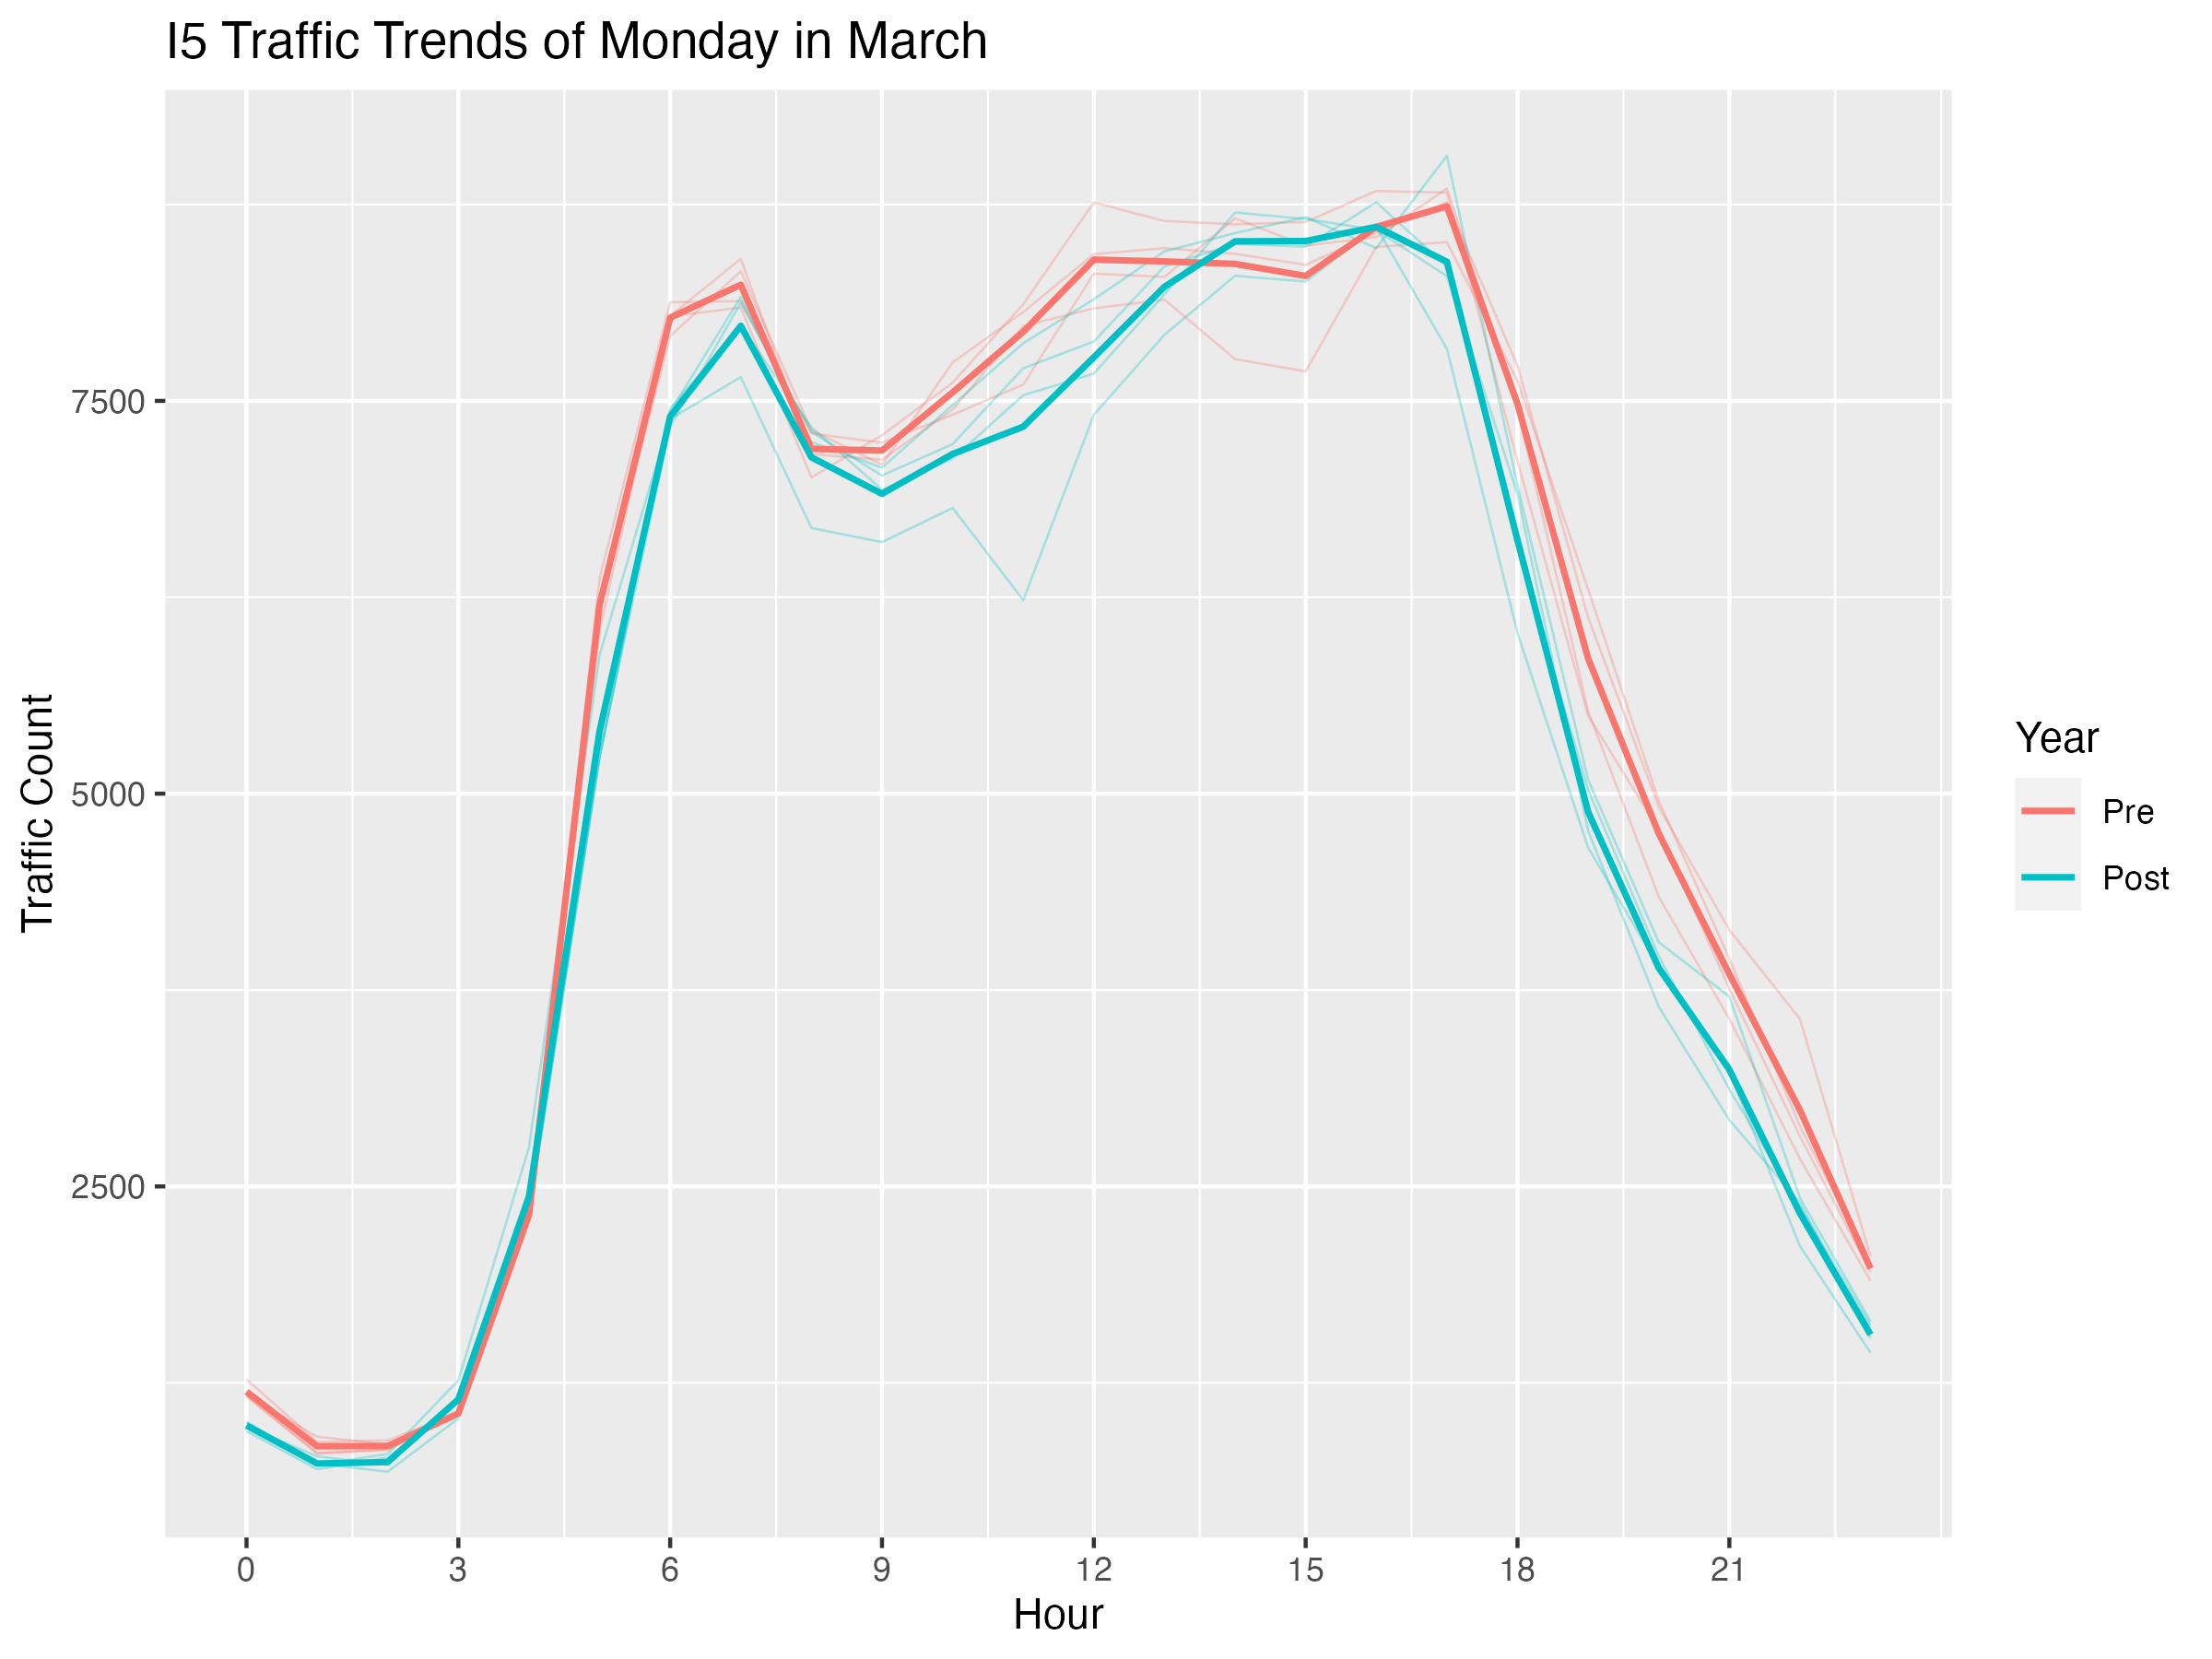
\includegraphics[width=\textwidth]{ATR26004_Plots/picture2_A04.png}
	\end{subfigure}
	\hfill
	\begin{subfigure}[b]{0.45\textwidth}
		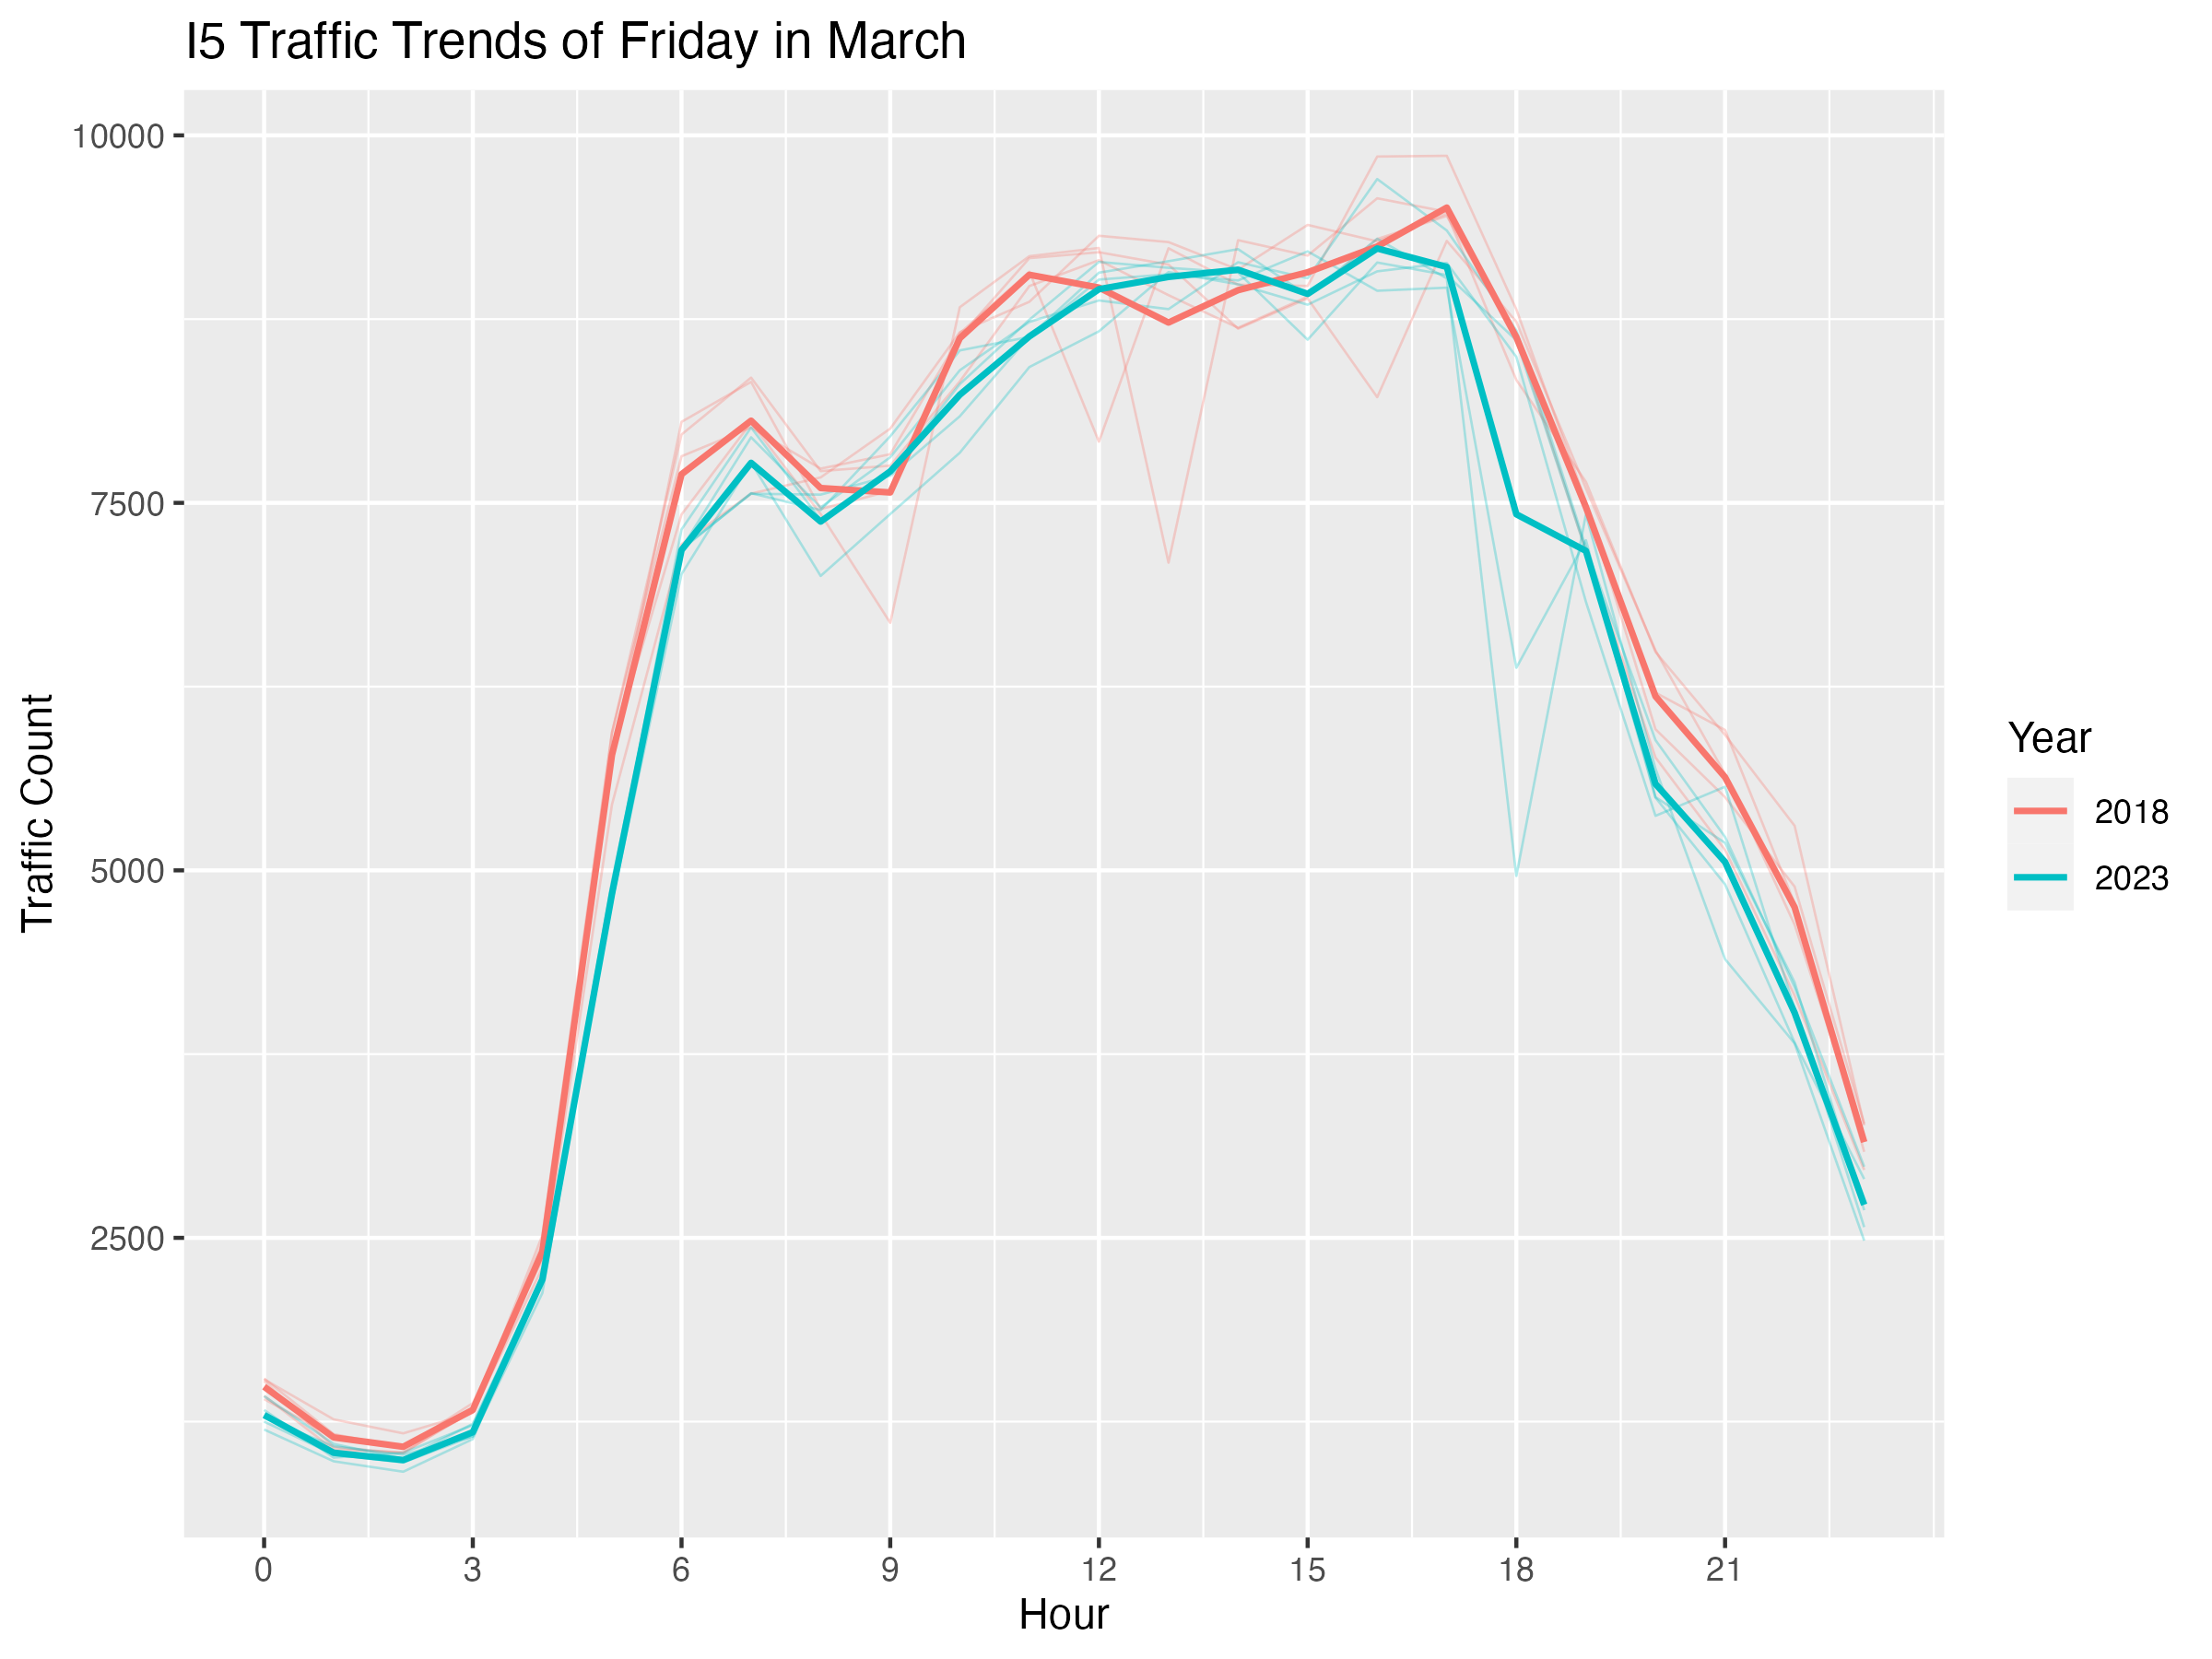
\includegraphics[width=\textwidth]{ATR26004_Plots/picture12_A04.png}
	\end{subfigure}
\end{figure}

\begin{figure}[H]
	\centering
	\begin{subfigure}[b]{0.45\textwidth}
		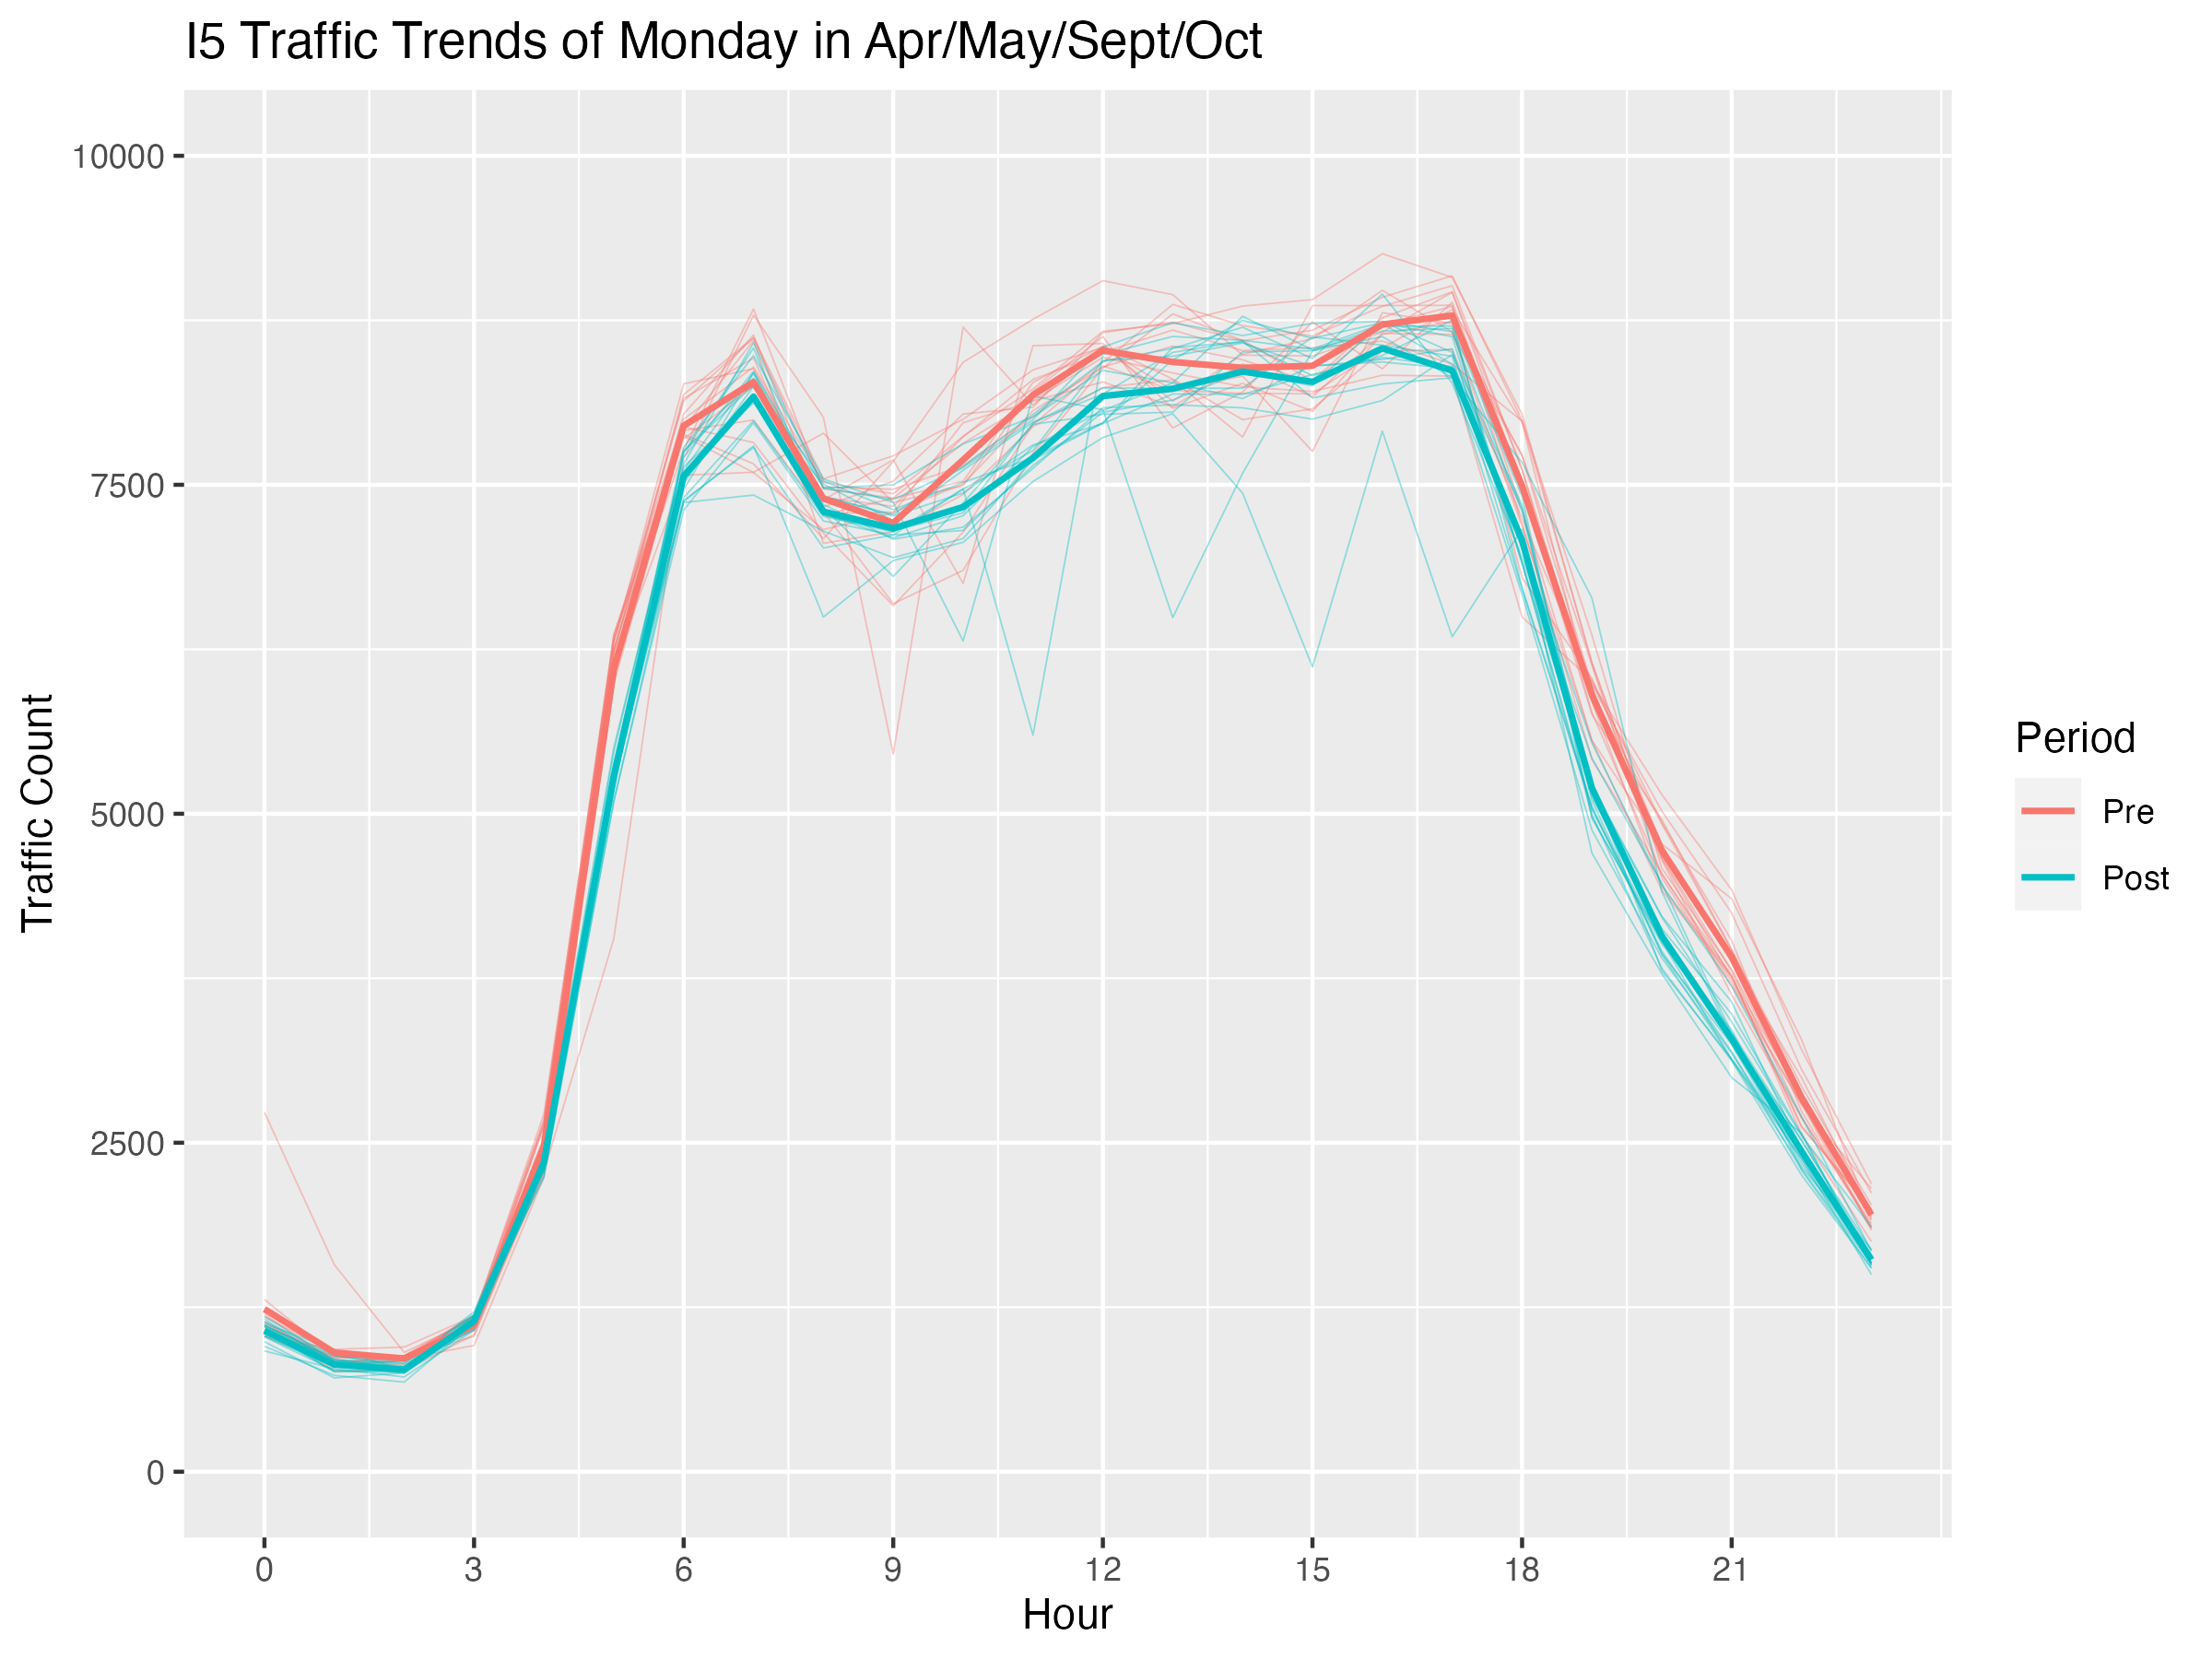
\includegraphics[width=\textwidth]{ATR26004_Plots/picture3_A04.png}
	\end{subfigure}
	\hfill
	\begin{subfigure}[b]{0.45\textwidth}
		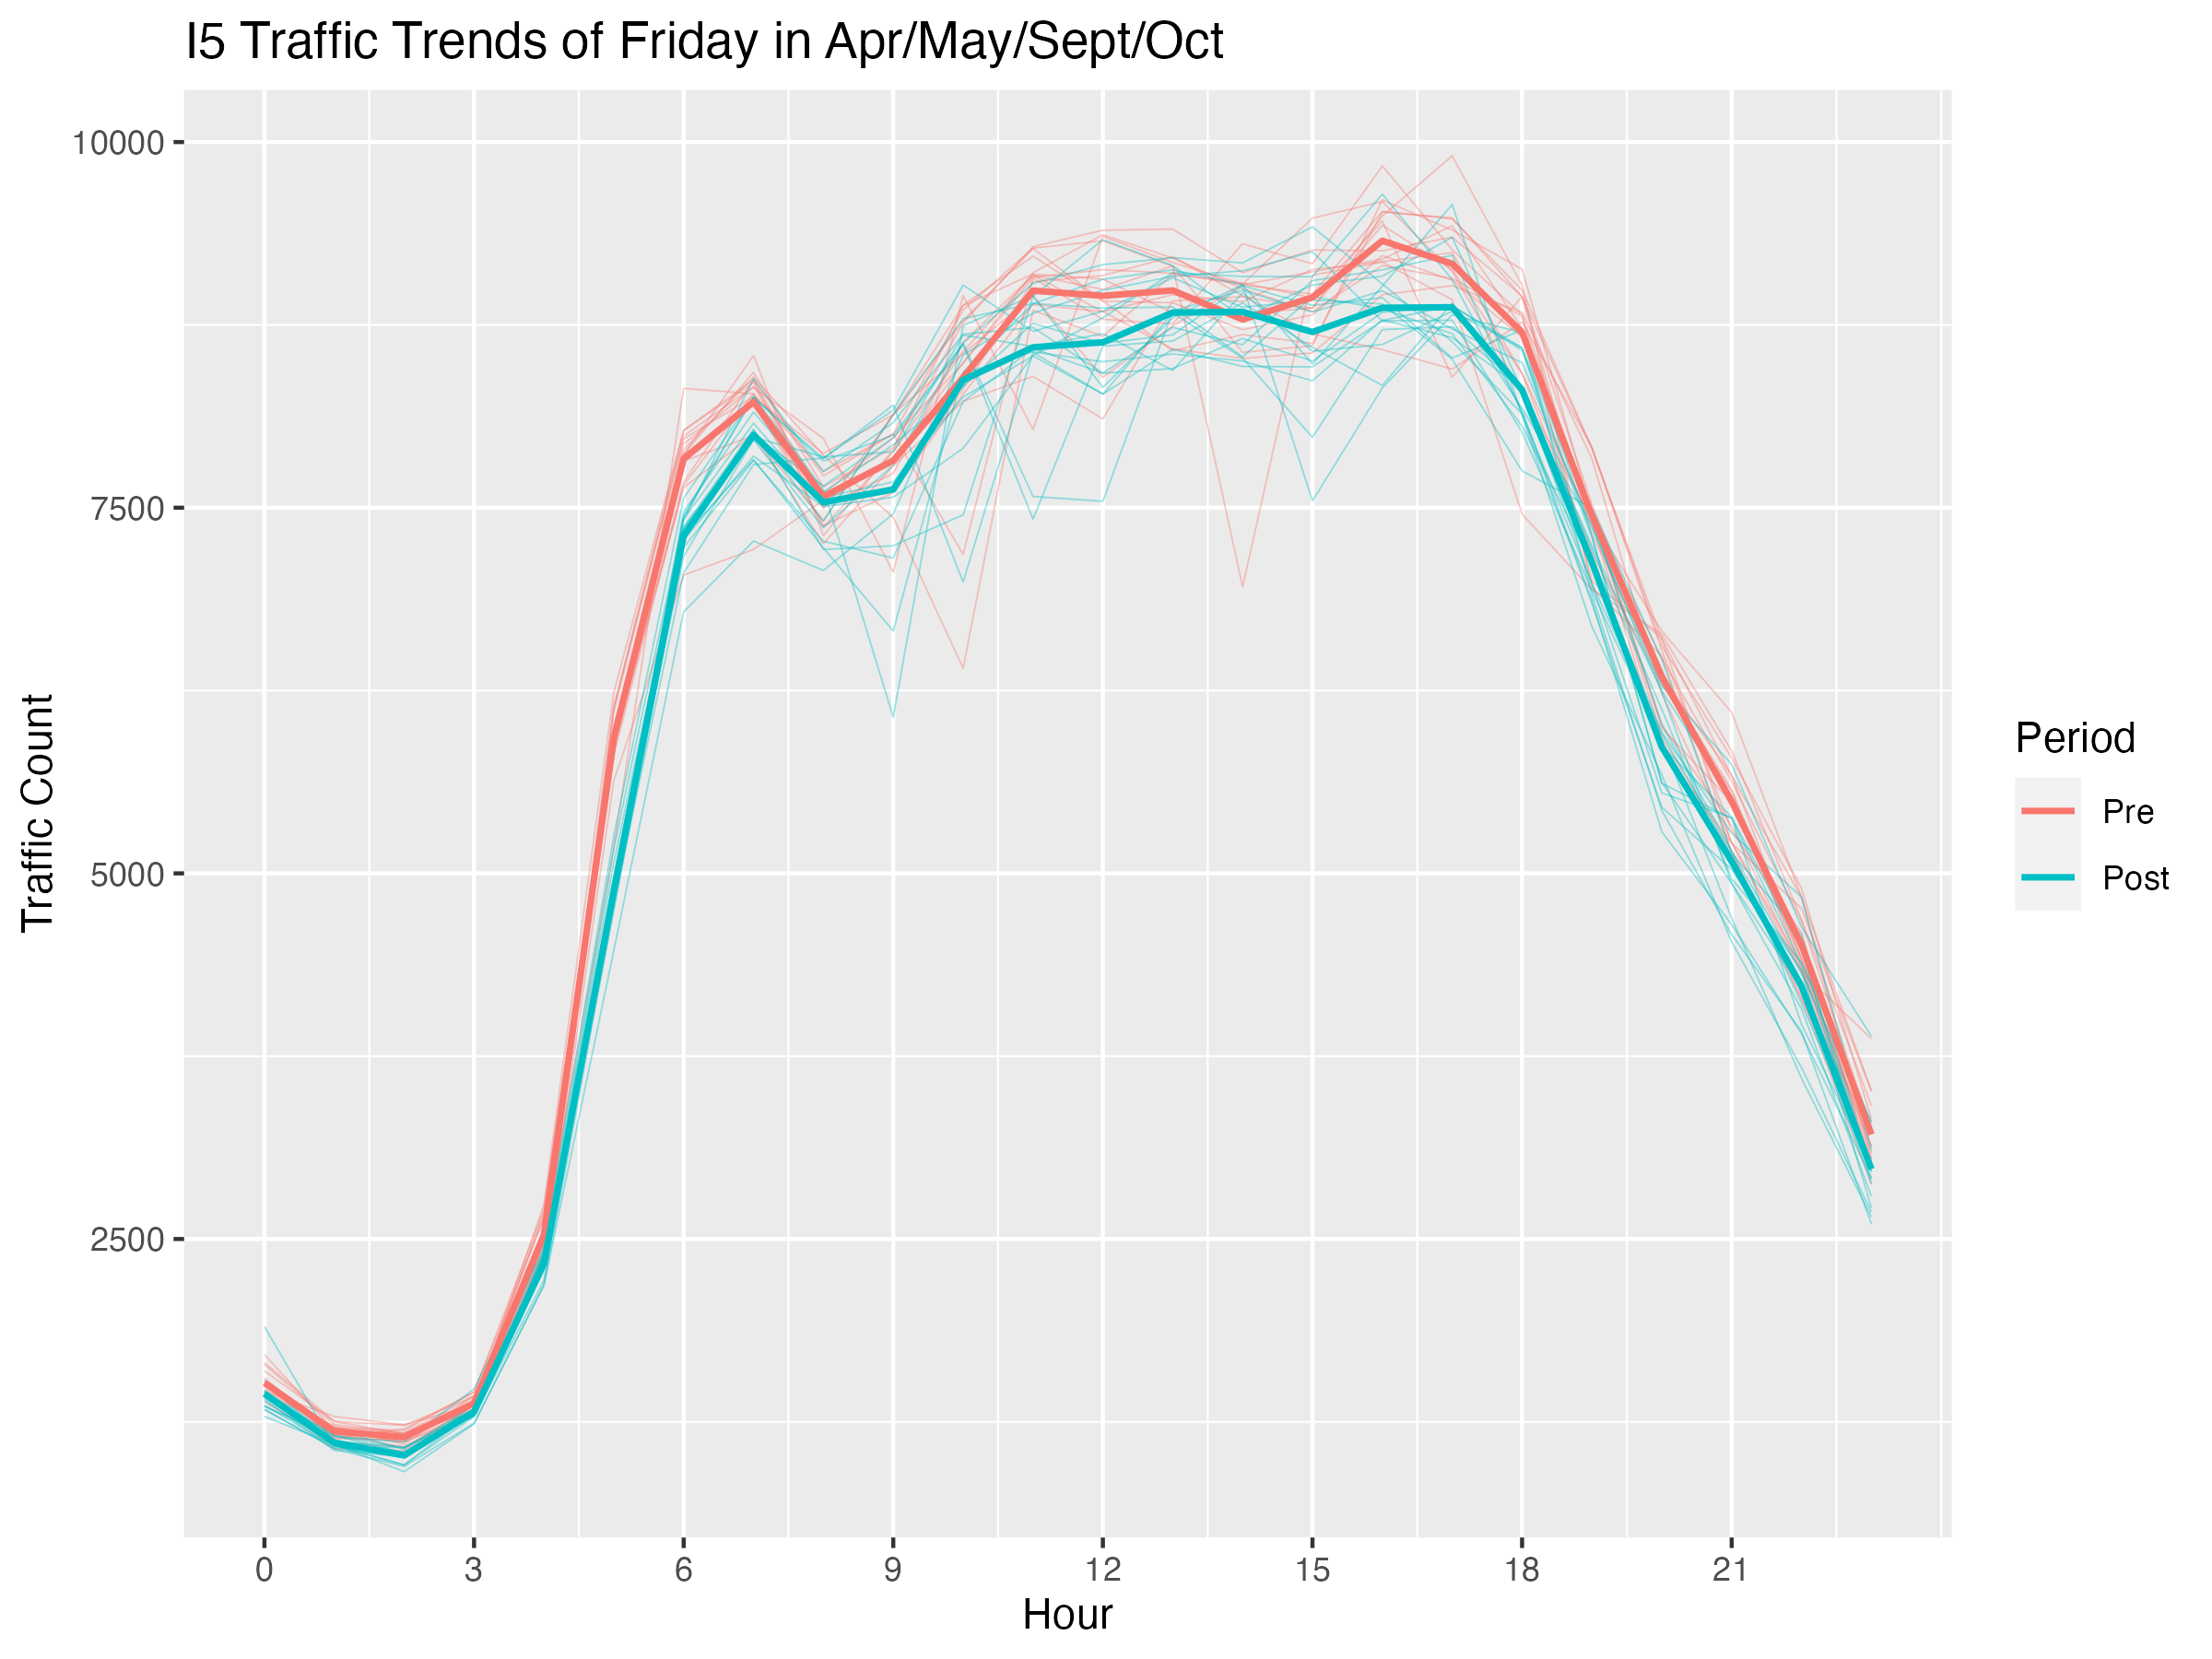
\includegraphics[width=\textwidth]{ATR26004_Plots/picture13_A04.png}
	\end{subfigure}
\end{figure}

\begin{figure}[H]
	\centering
	\begin{subfigure}[b]{0.45\textwidth}
		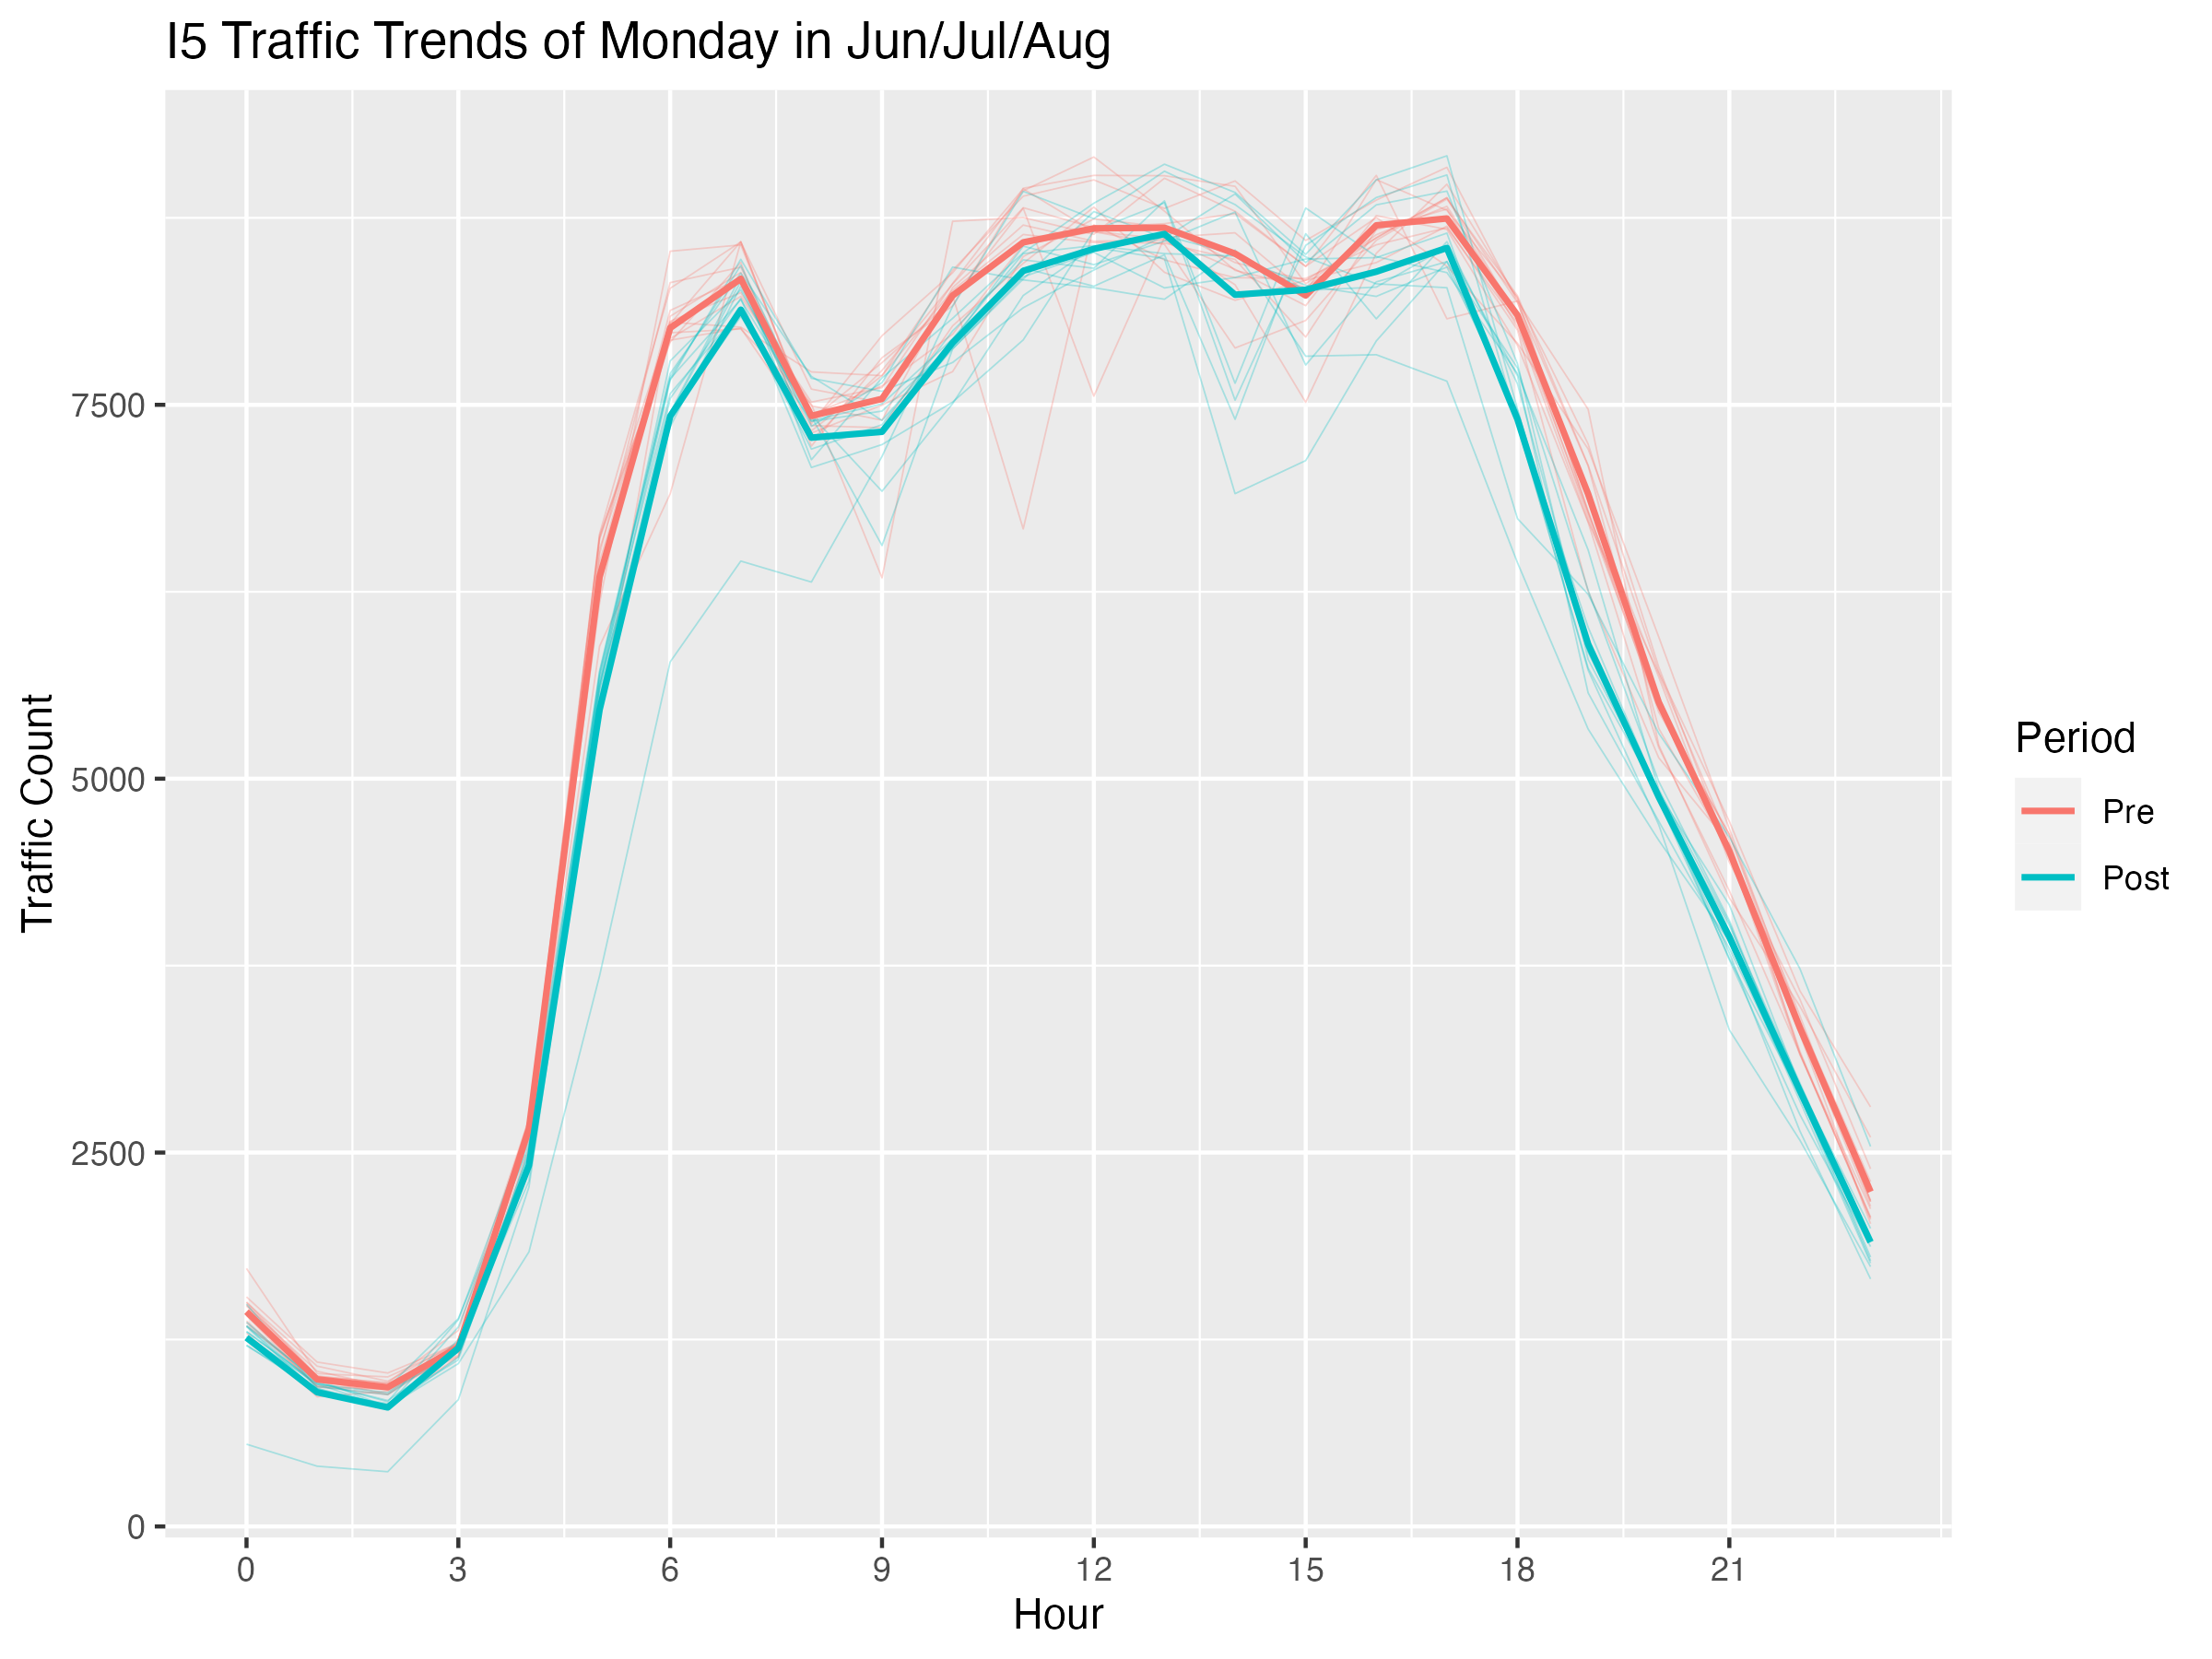
\includegraphics[width=\textwidth]{ATR26004_Plots/picture4_A04.png}
	\end{subfigure}
	\hfill
	\begin{subfigure}[b]{0.45\textwidth}
		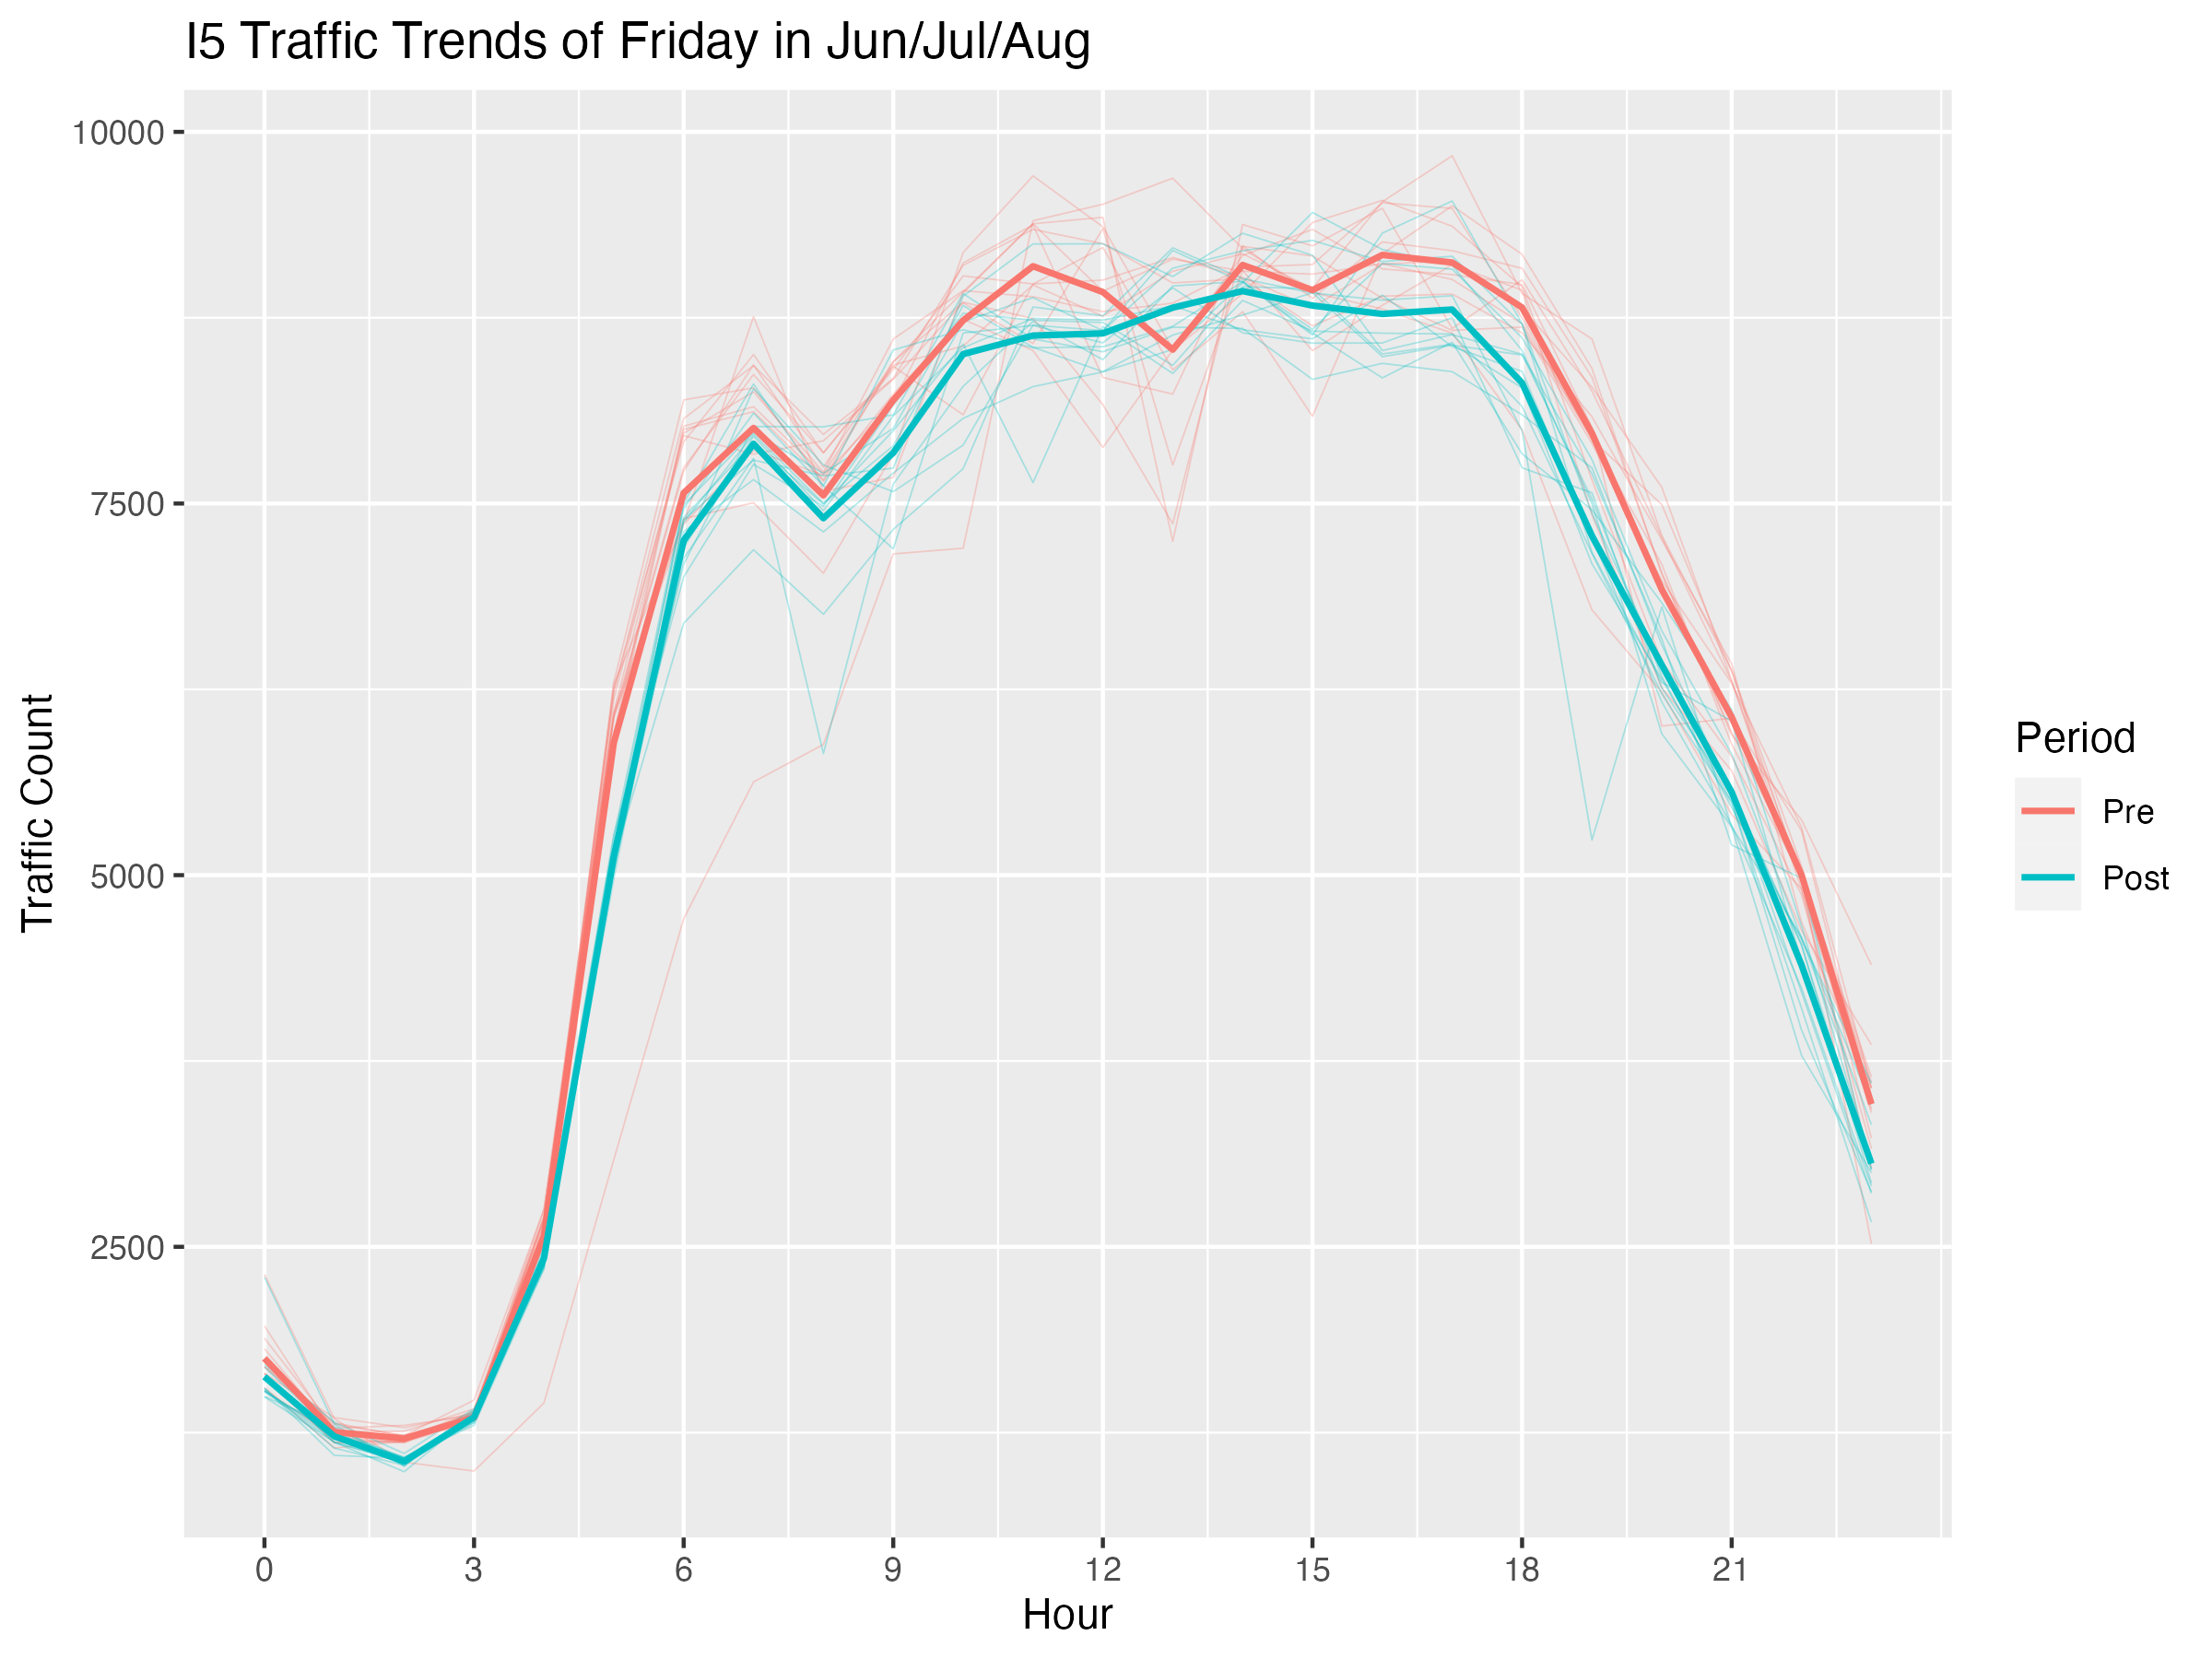
\includegraphics[width=\textwidth]{ATR26004_Plots/picture14_A04.png}
	\end{subfigure}
\end{figure}

\begin{figure}[H]
	\centering
	\begin{subfigure}[b]{0.45\textwidth}
		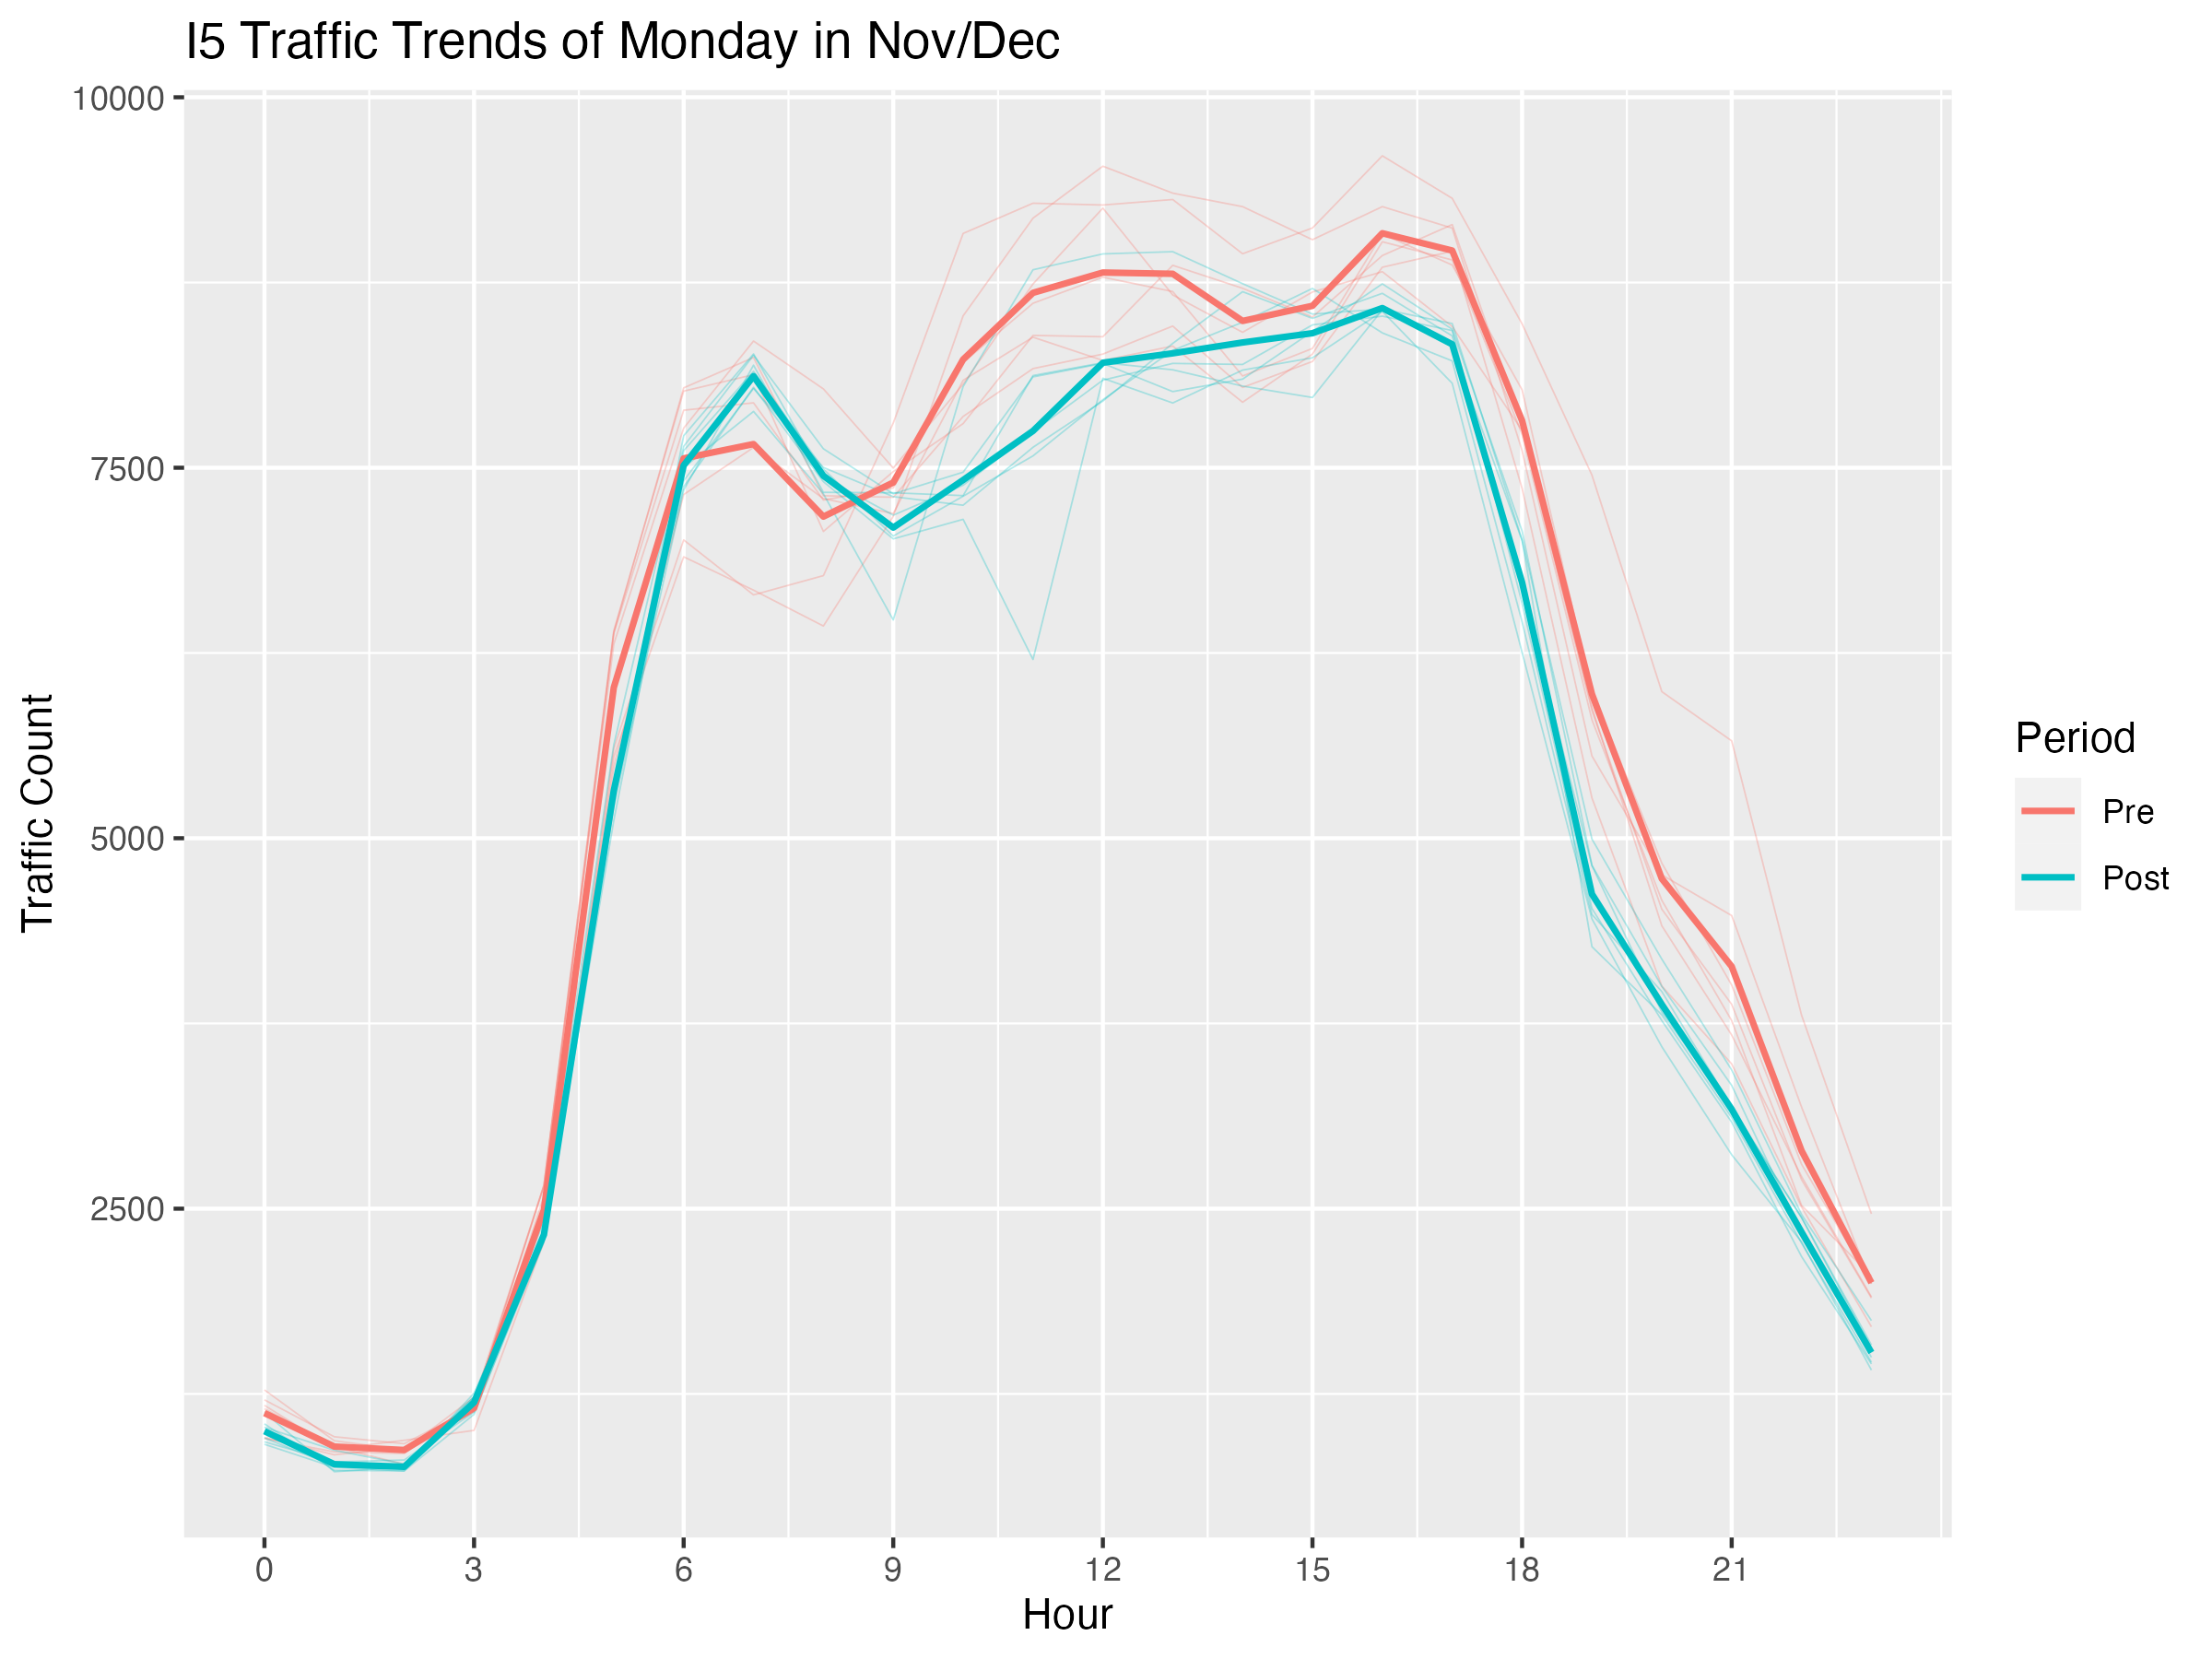
\includegraphics[width=\textwidth]{ATR26004_Plots/picture5_A04.png}
	\end{subfigure}
	\hfill
	\begin{subfigure}[b]{0.45\textwidth}
		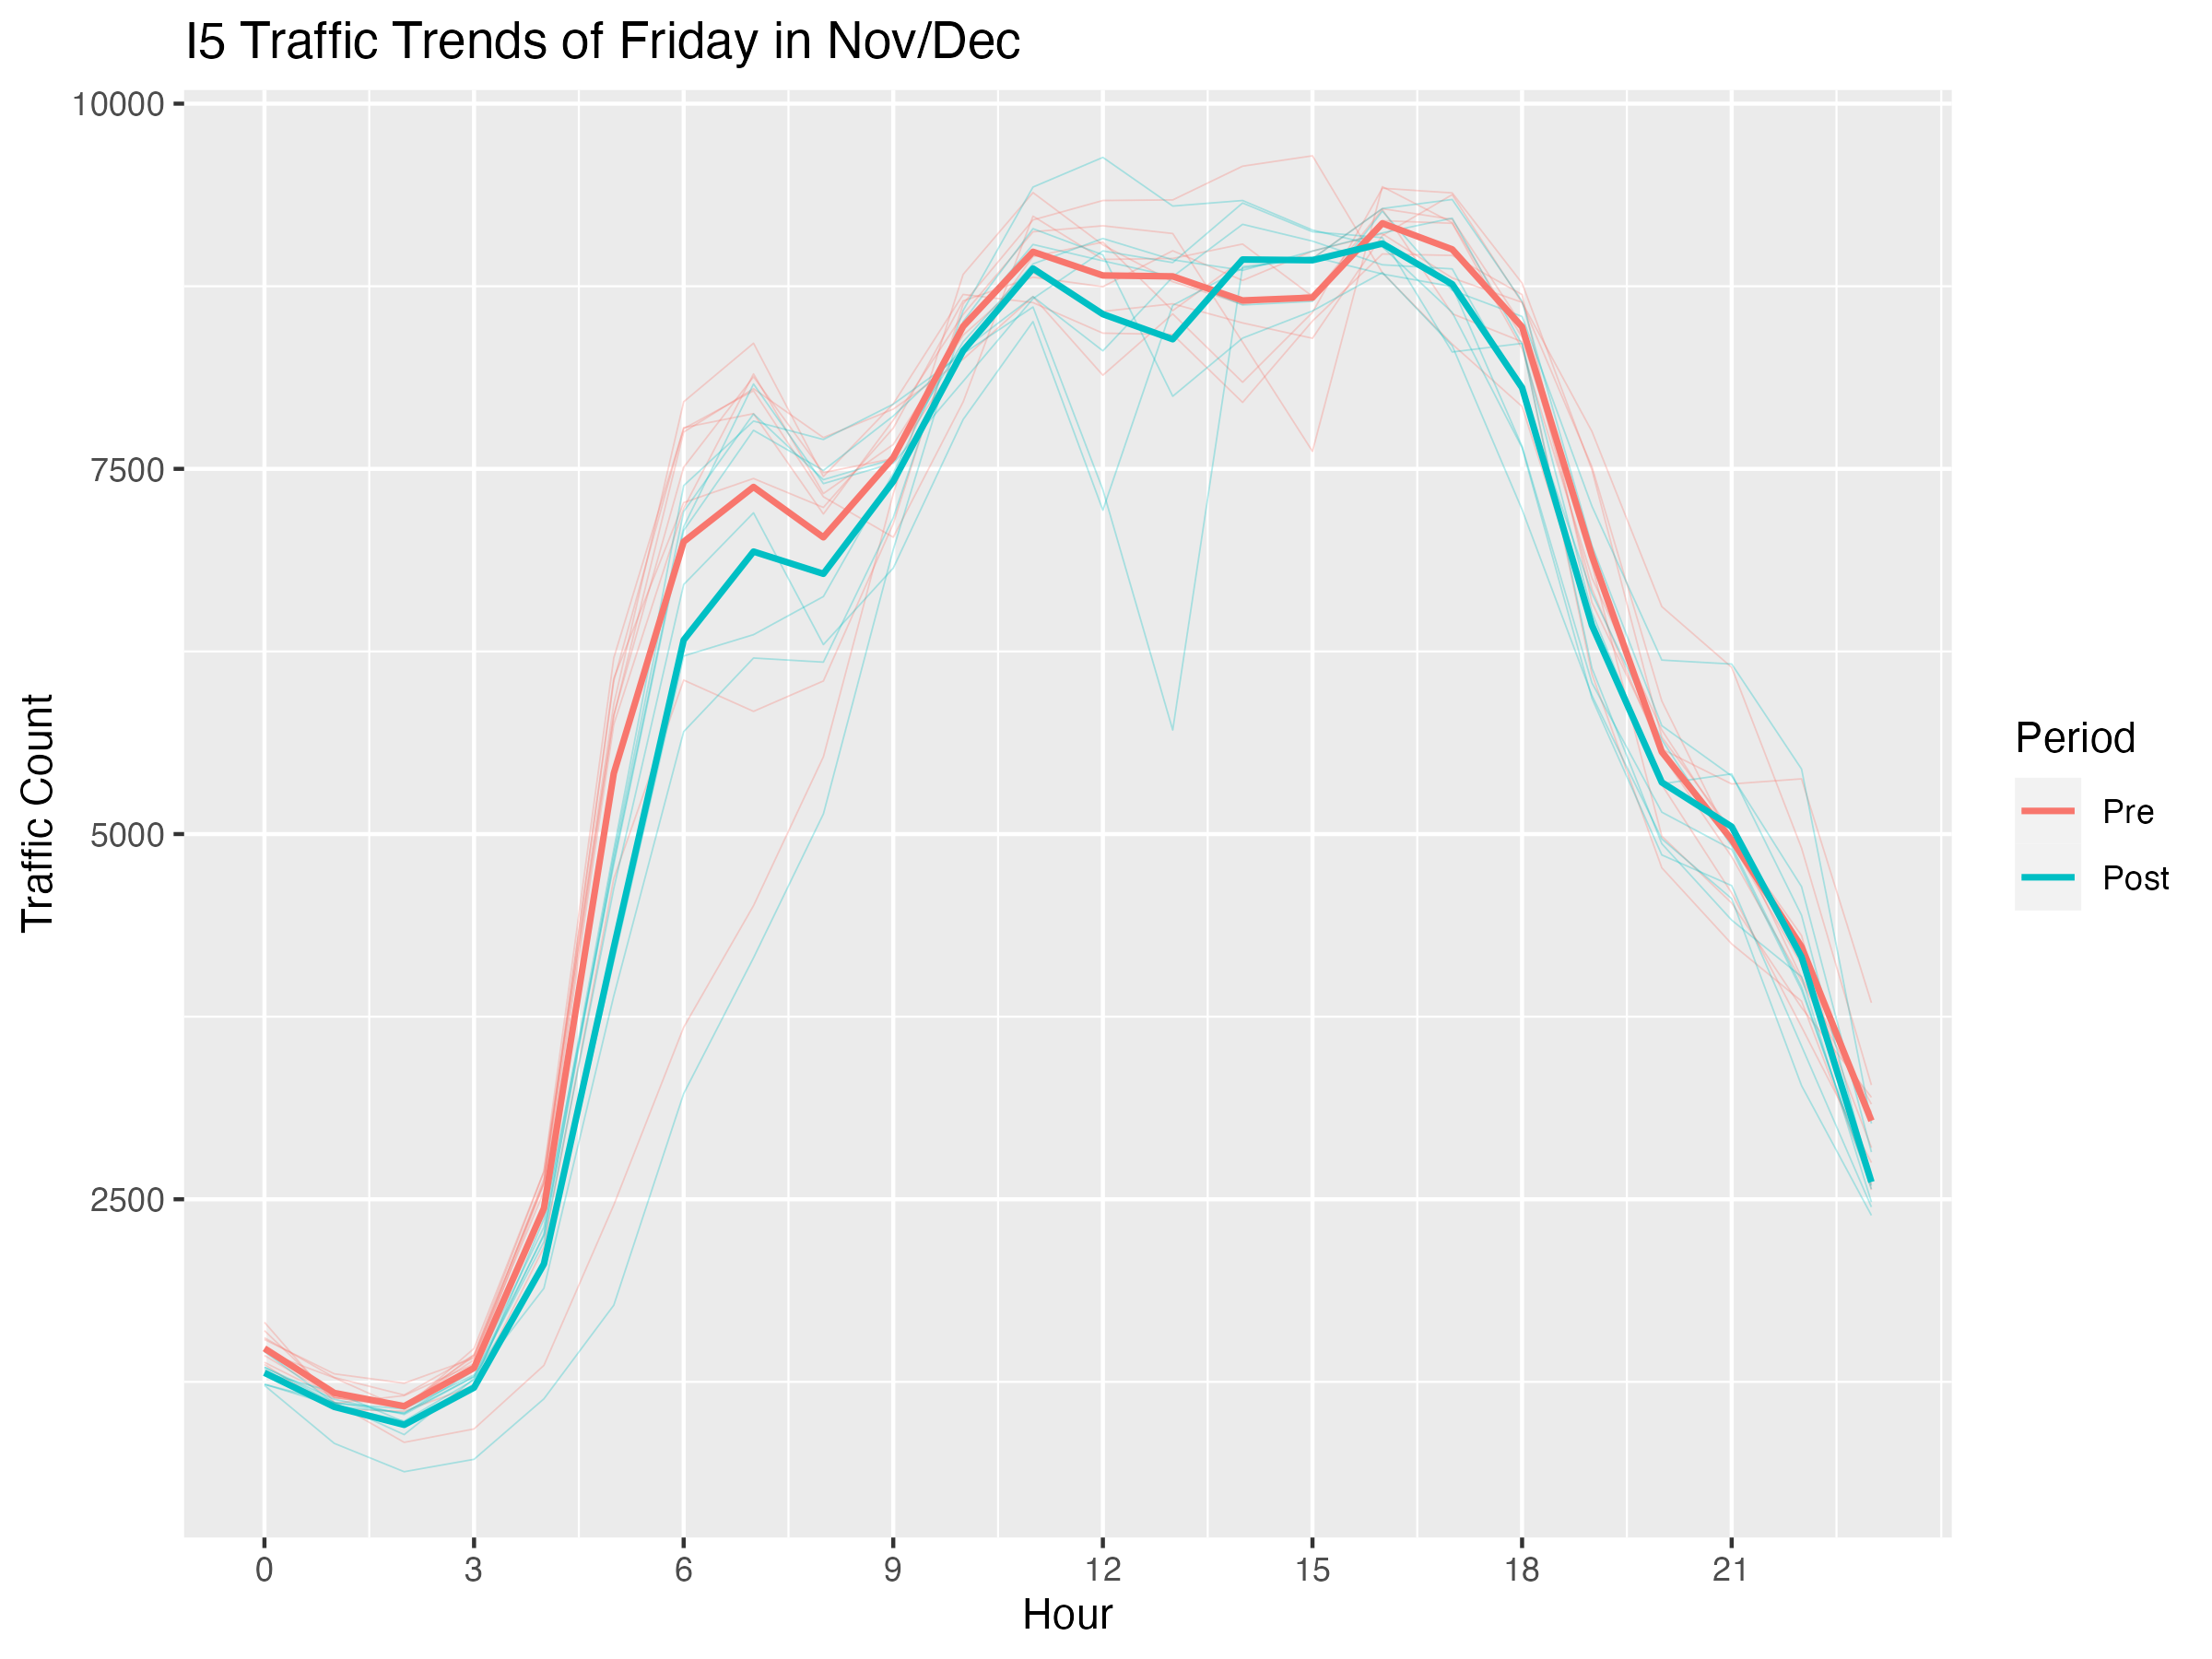
\includegraphics[width=\textwidth]{ATR26004_Plots/picture15_A04.png}
	\end{subfigure}
\end{figure}

\begin{figure}[H]
	\centering
	\begin{subfigure}[b]{0.45\textwidth}
		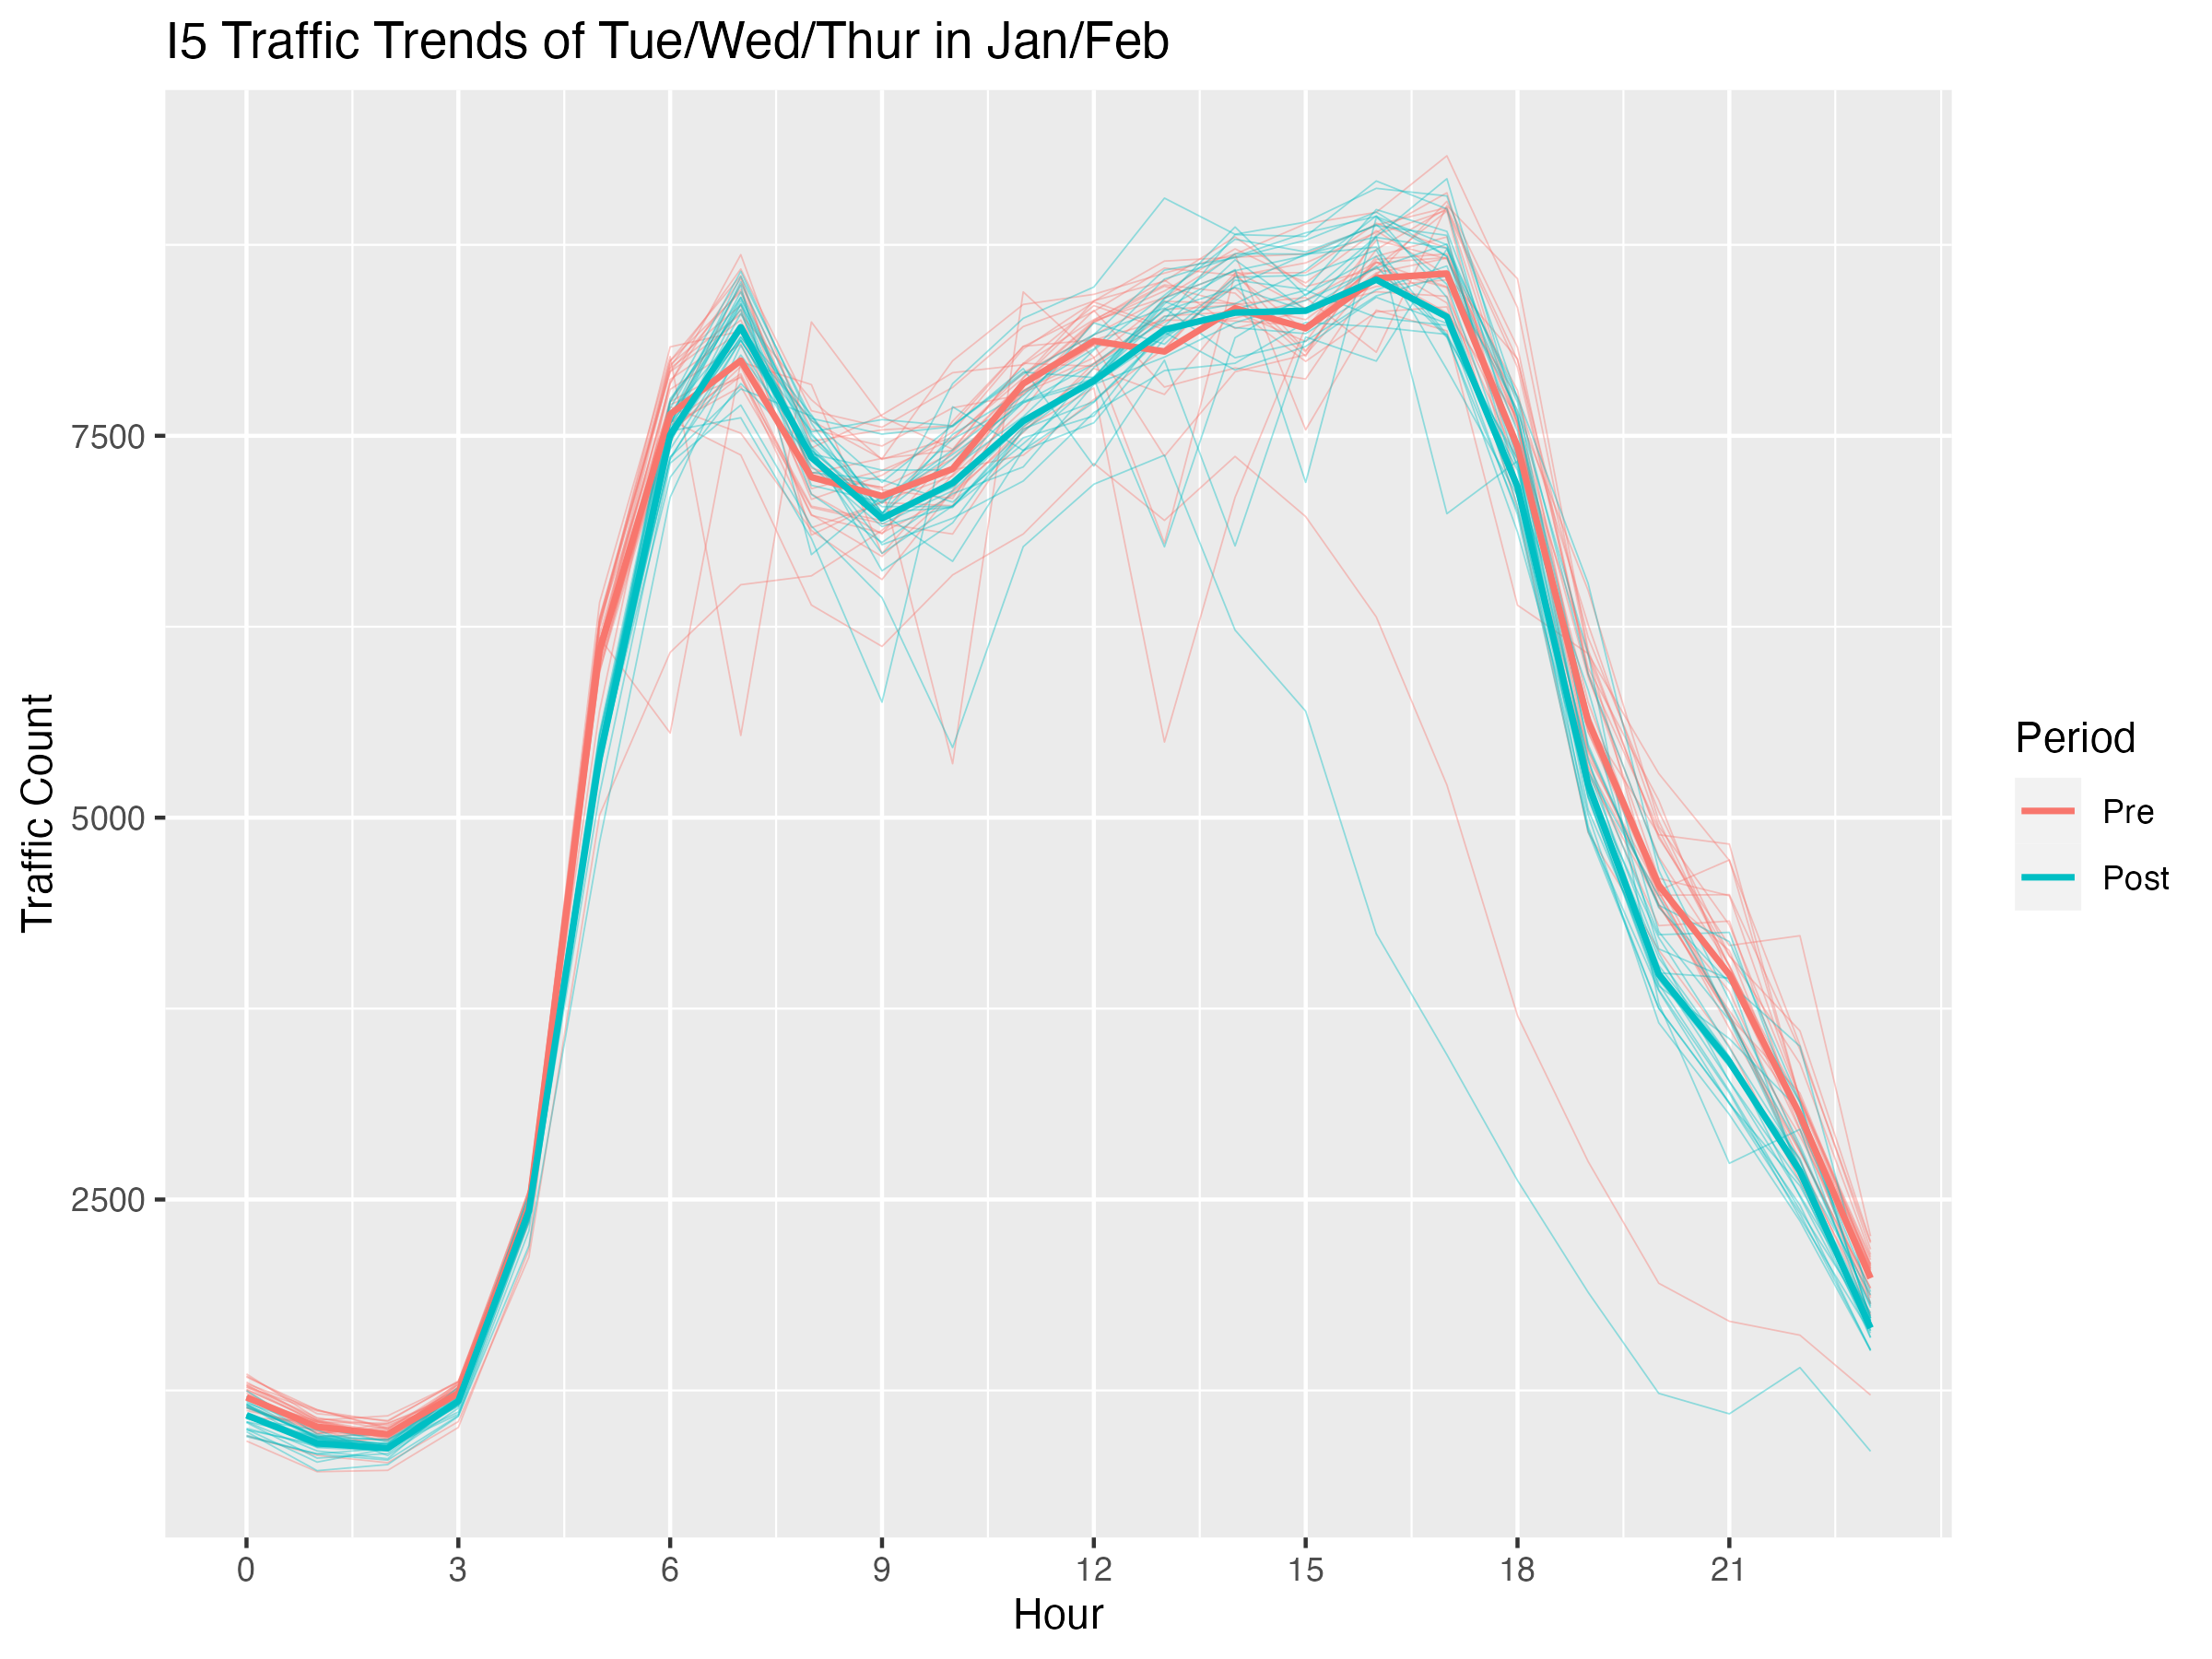
\includegraphics[width=\textwidth]{ATR26004_Plots/picture6_A04.png}
	\end{subfigure}
	\hfill
	\begin{subfigure}[b]{0.45\textwidth}
		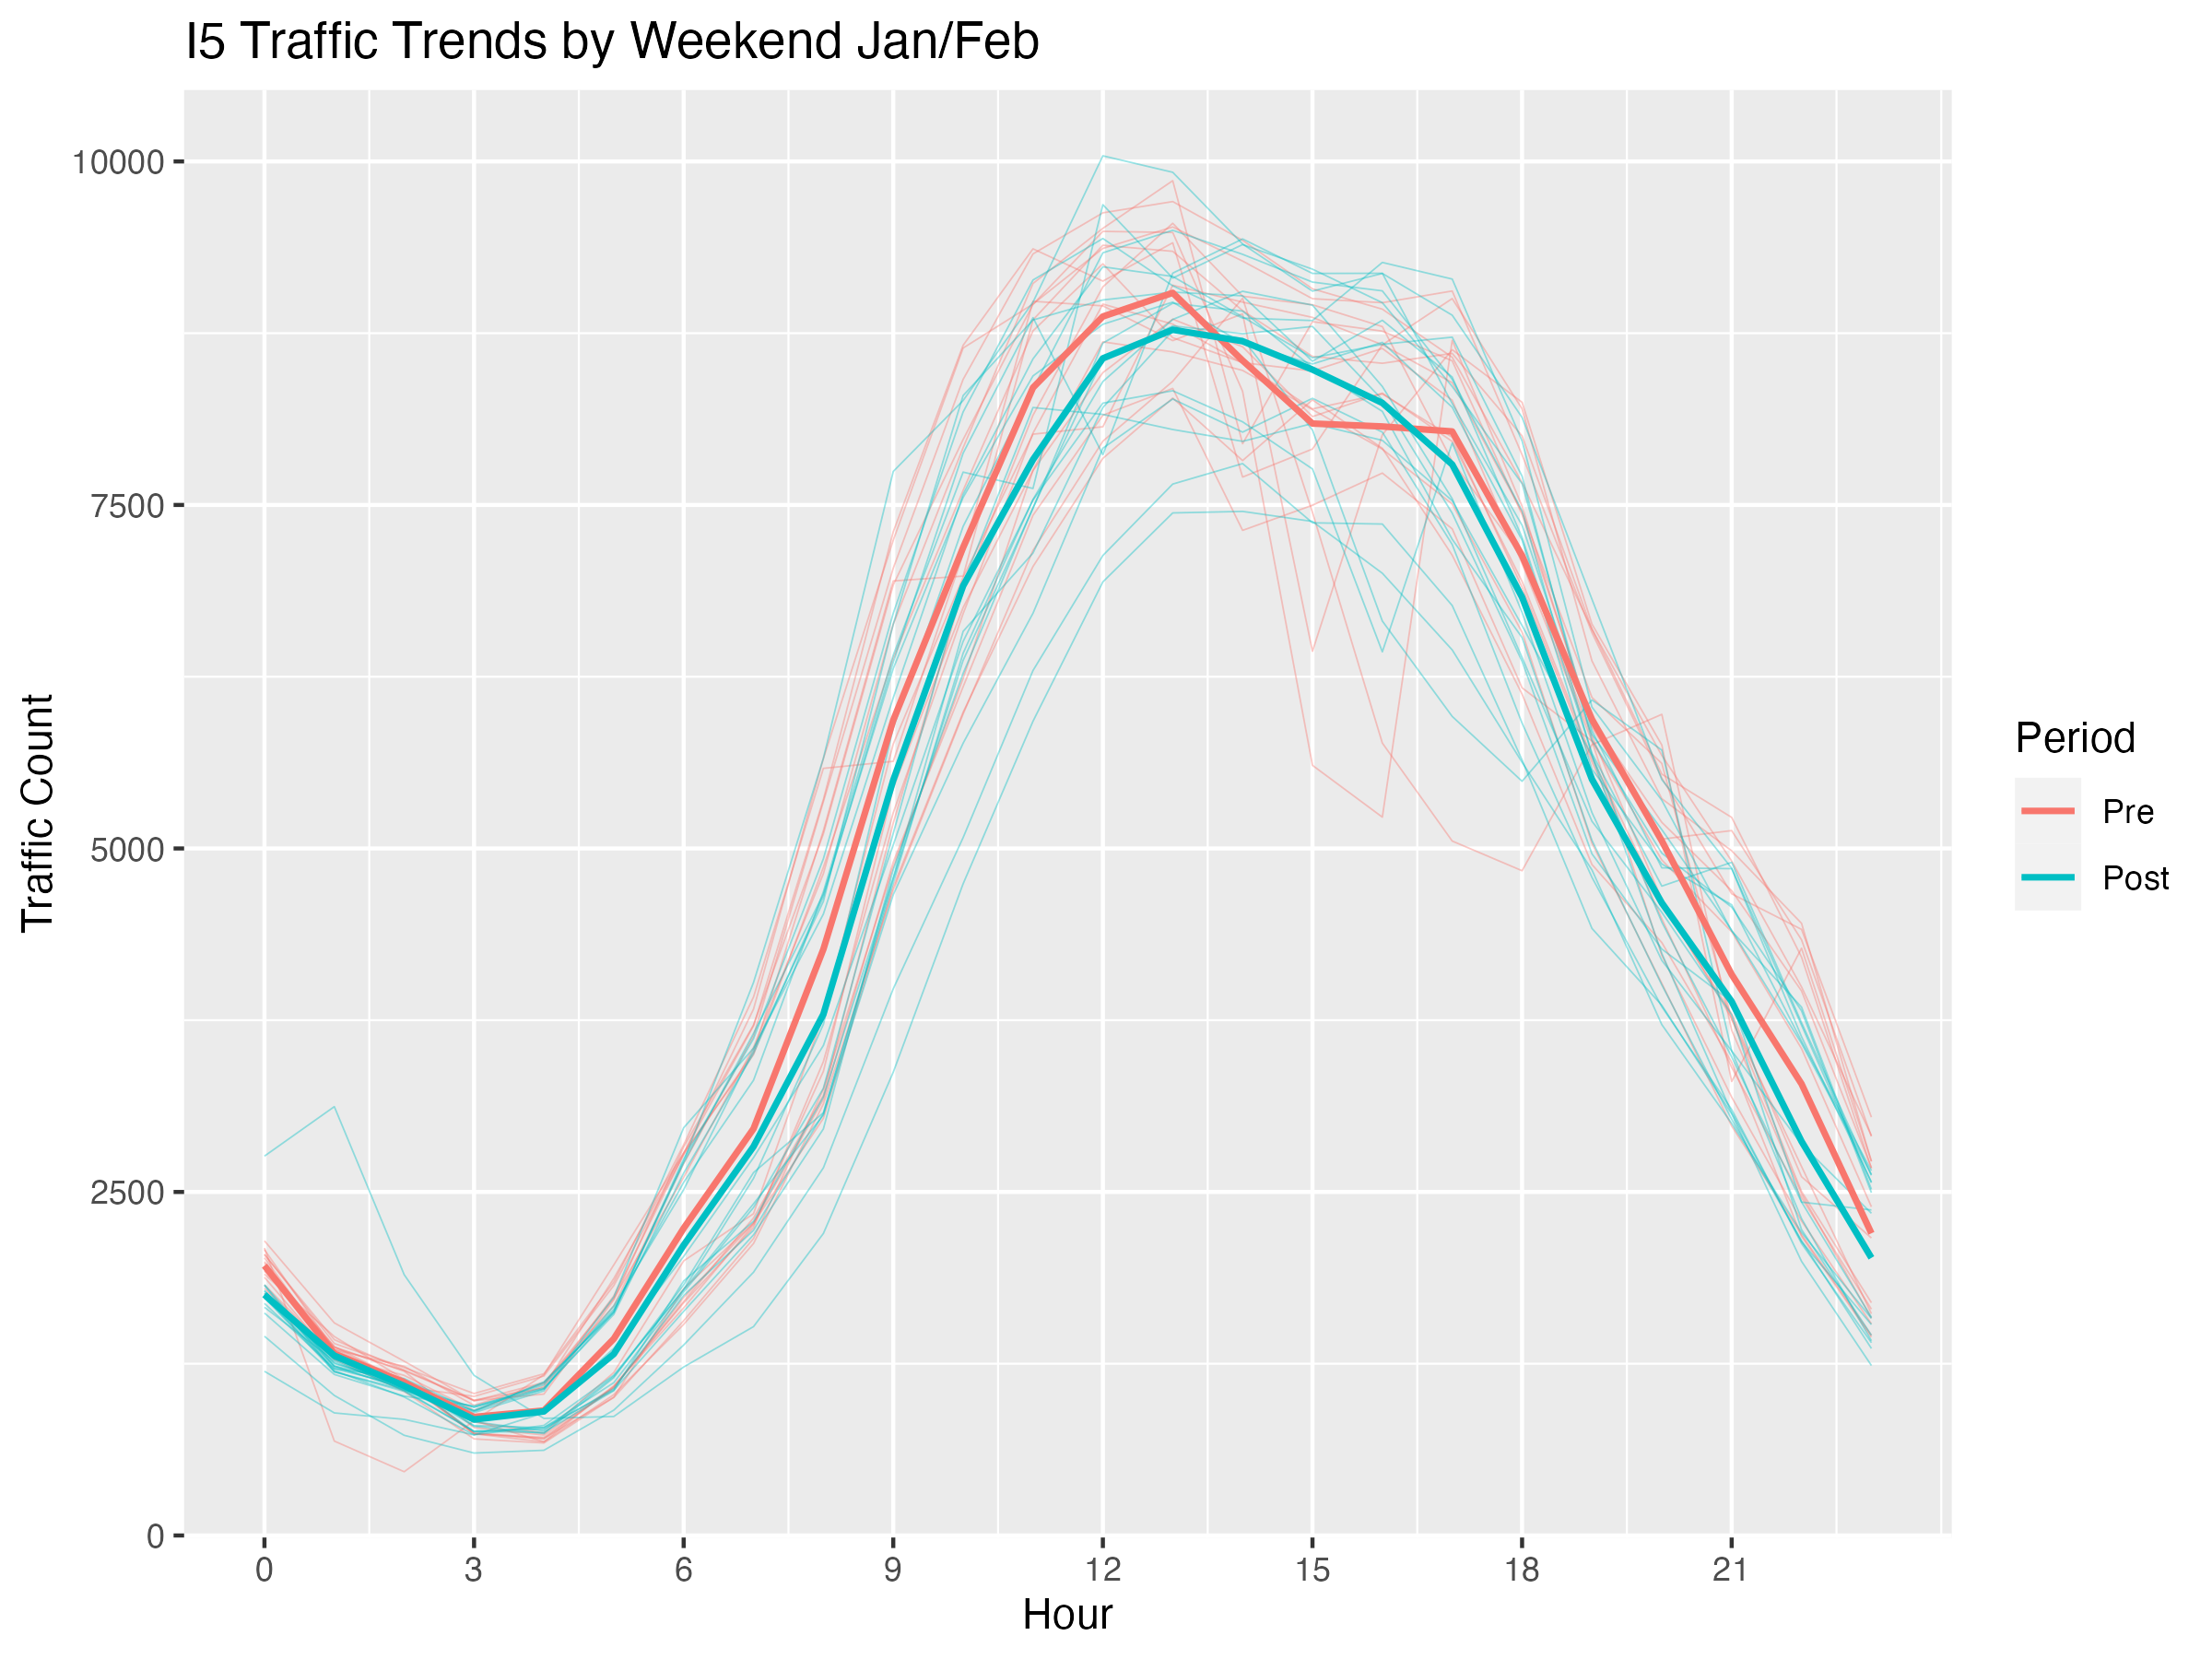
\includegraphics[width=\textwidth]{ATR26004_Plots/picture16_A04.png}
	\end{subfigure}
\end{figure}

\begin{figure}[H]
	\centering
	\begin{subfigure}[b]{0.45\textwidth}
		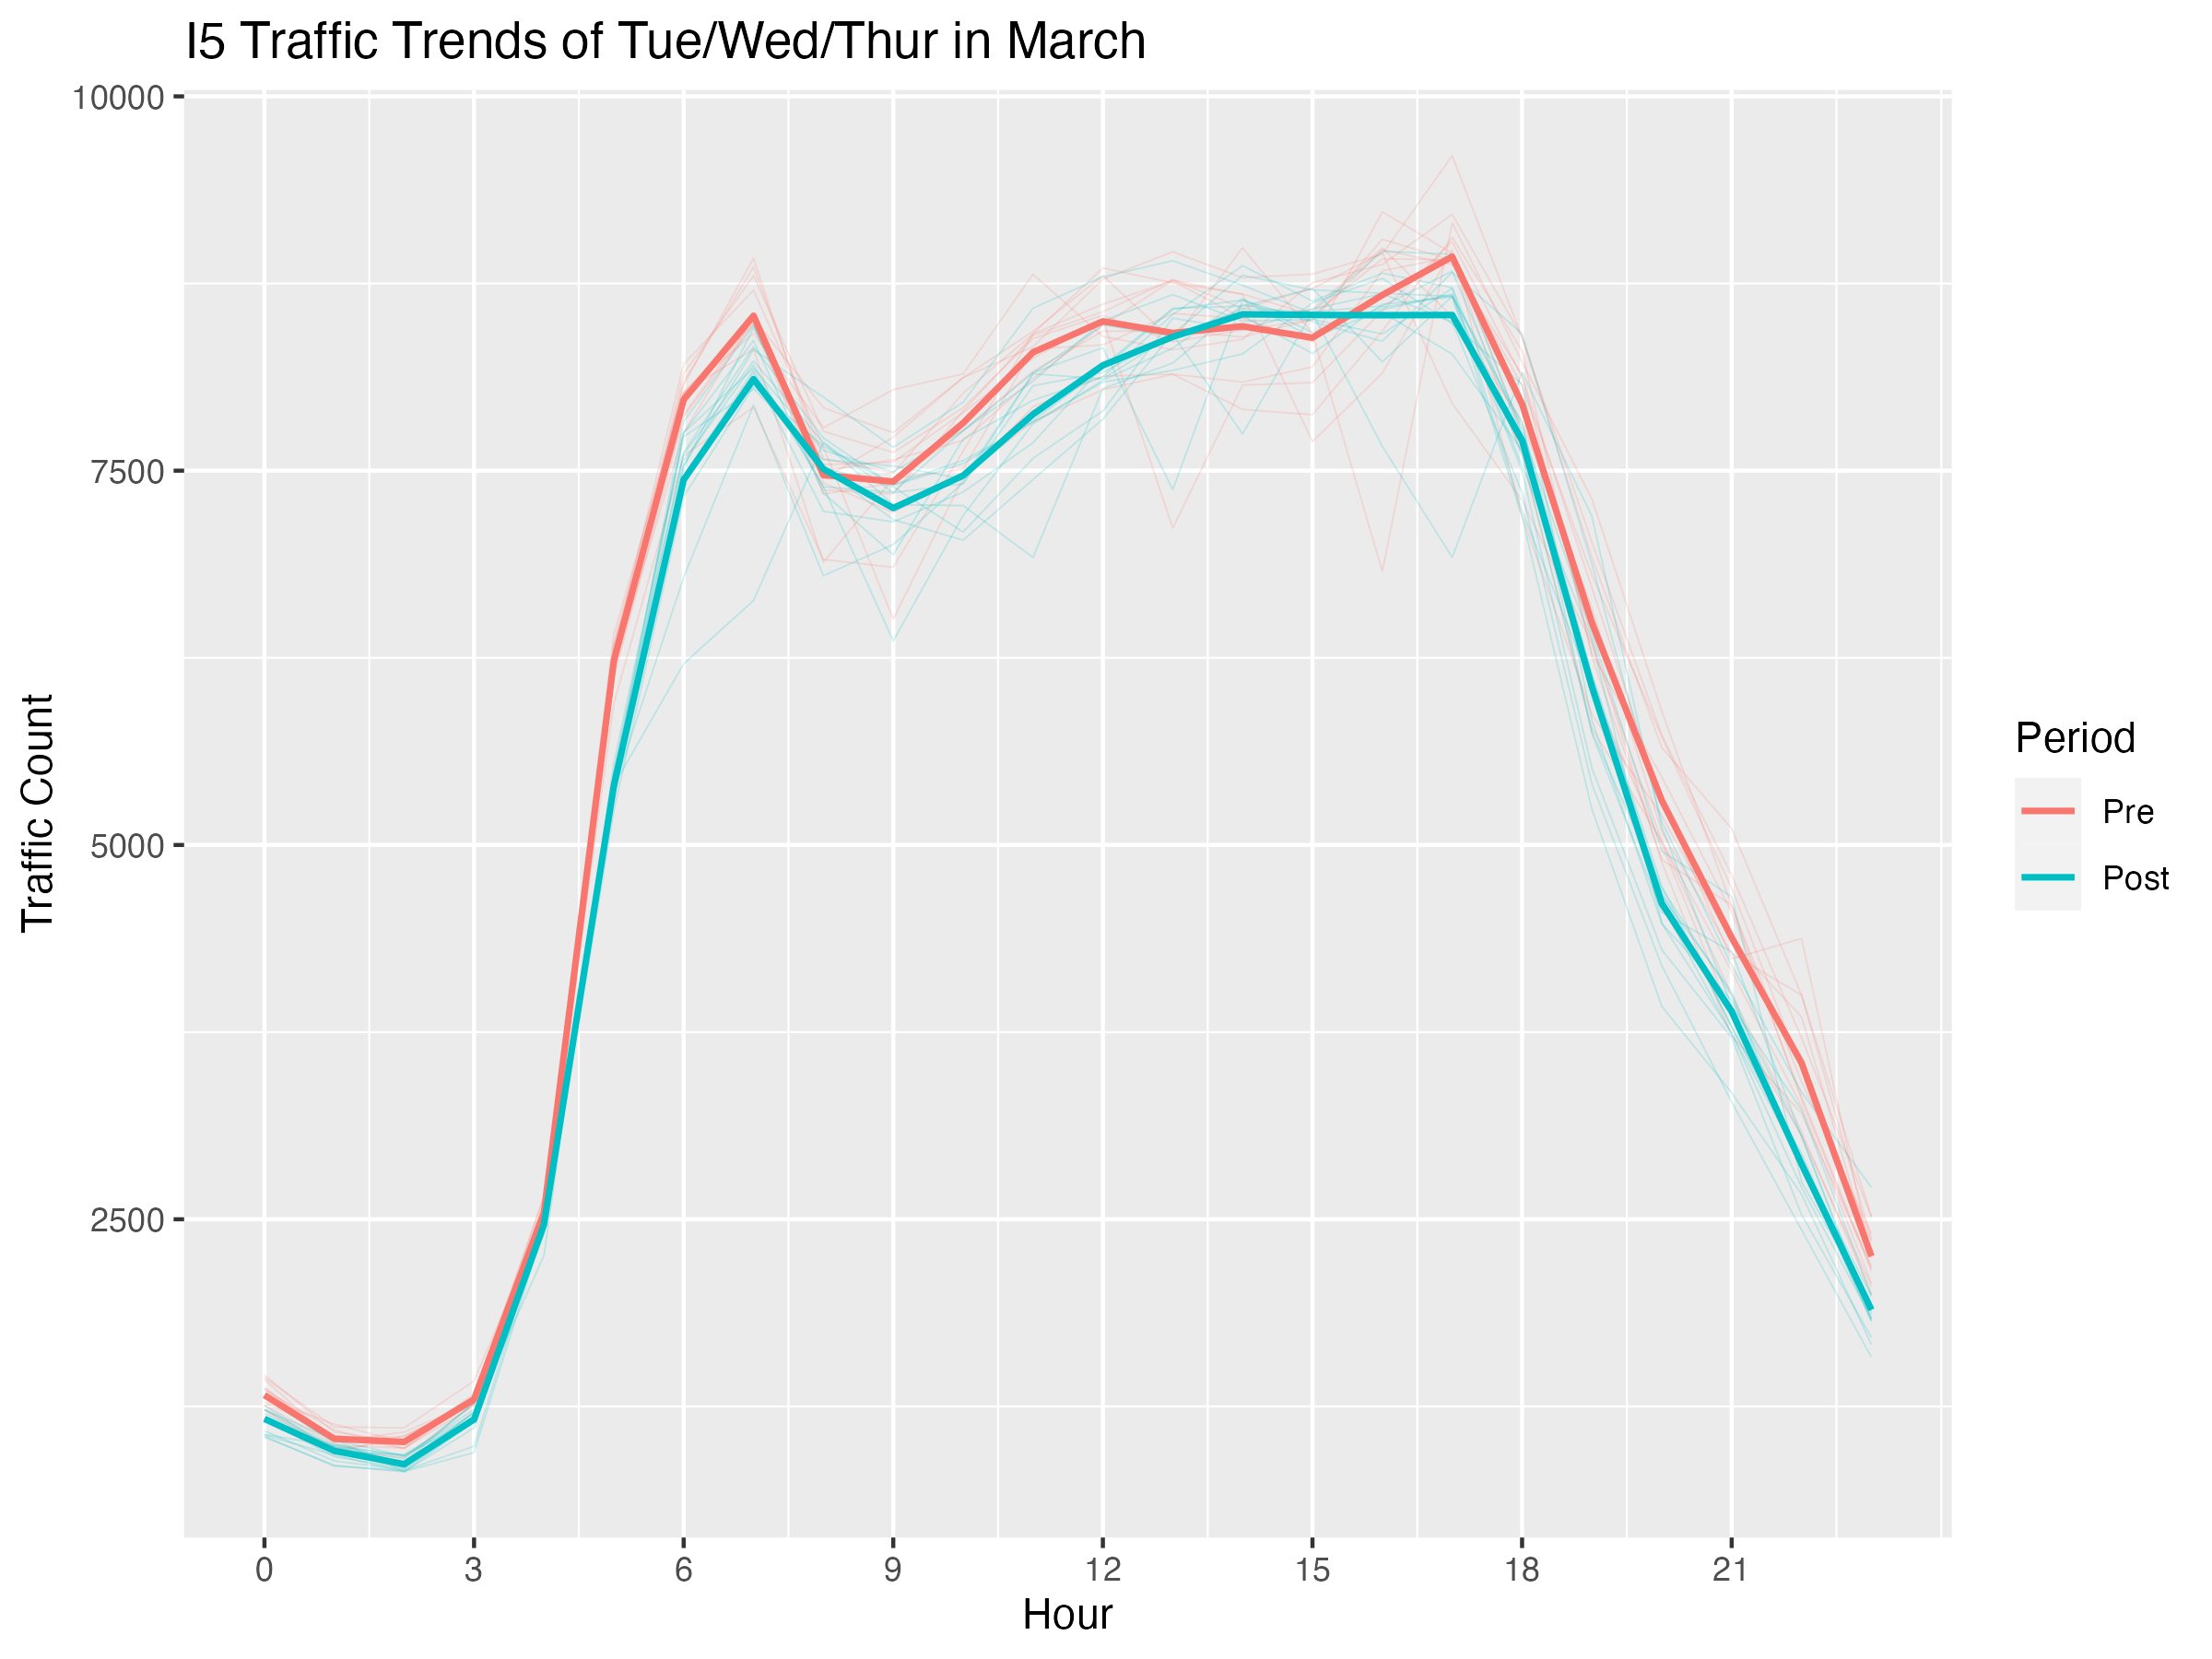
\includegraphics[width=\textwidth]{ATR26004_Plots/picture7_A04.png}
	\end{subfigure}
	\hfill
	\begin{subfigure}[b]{0.45\textwidth}
		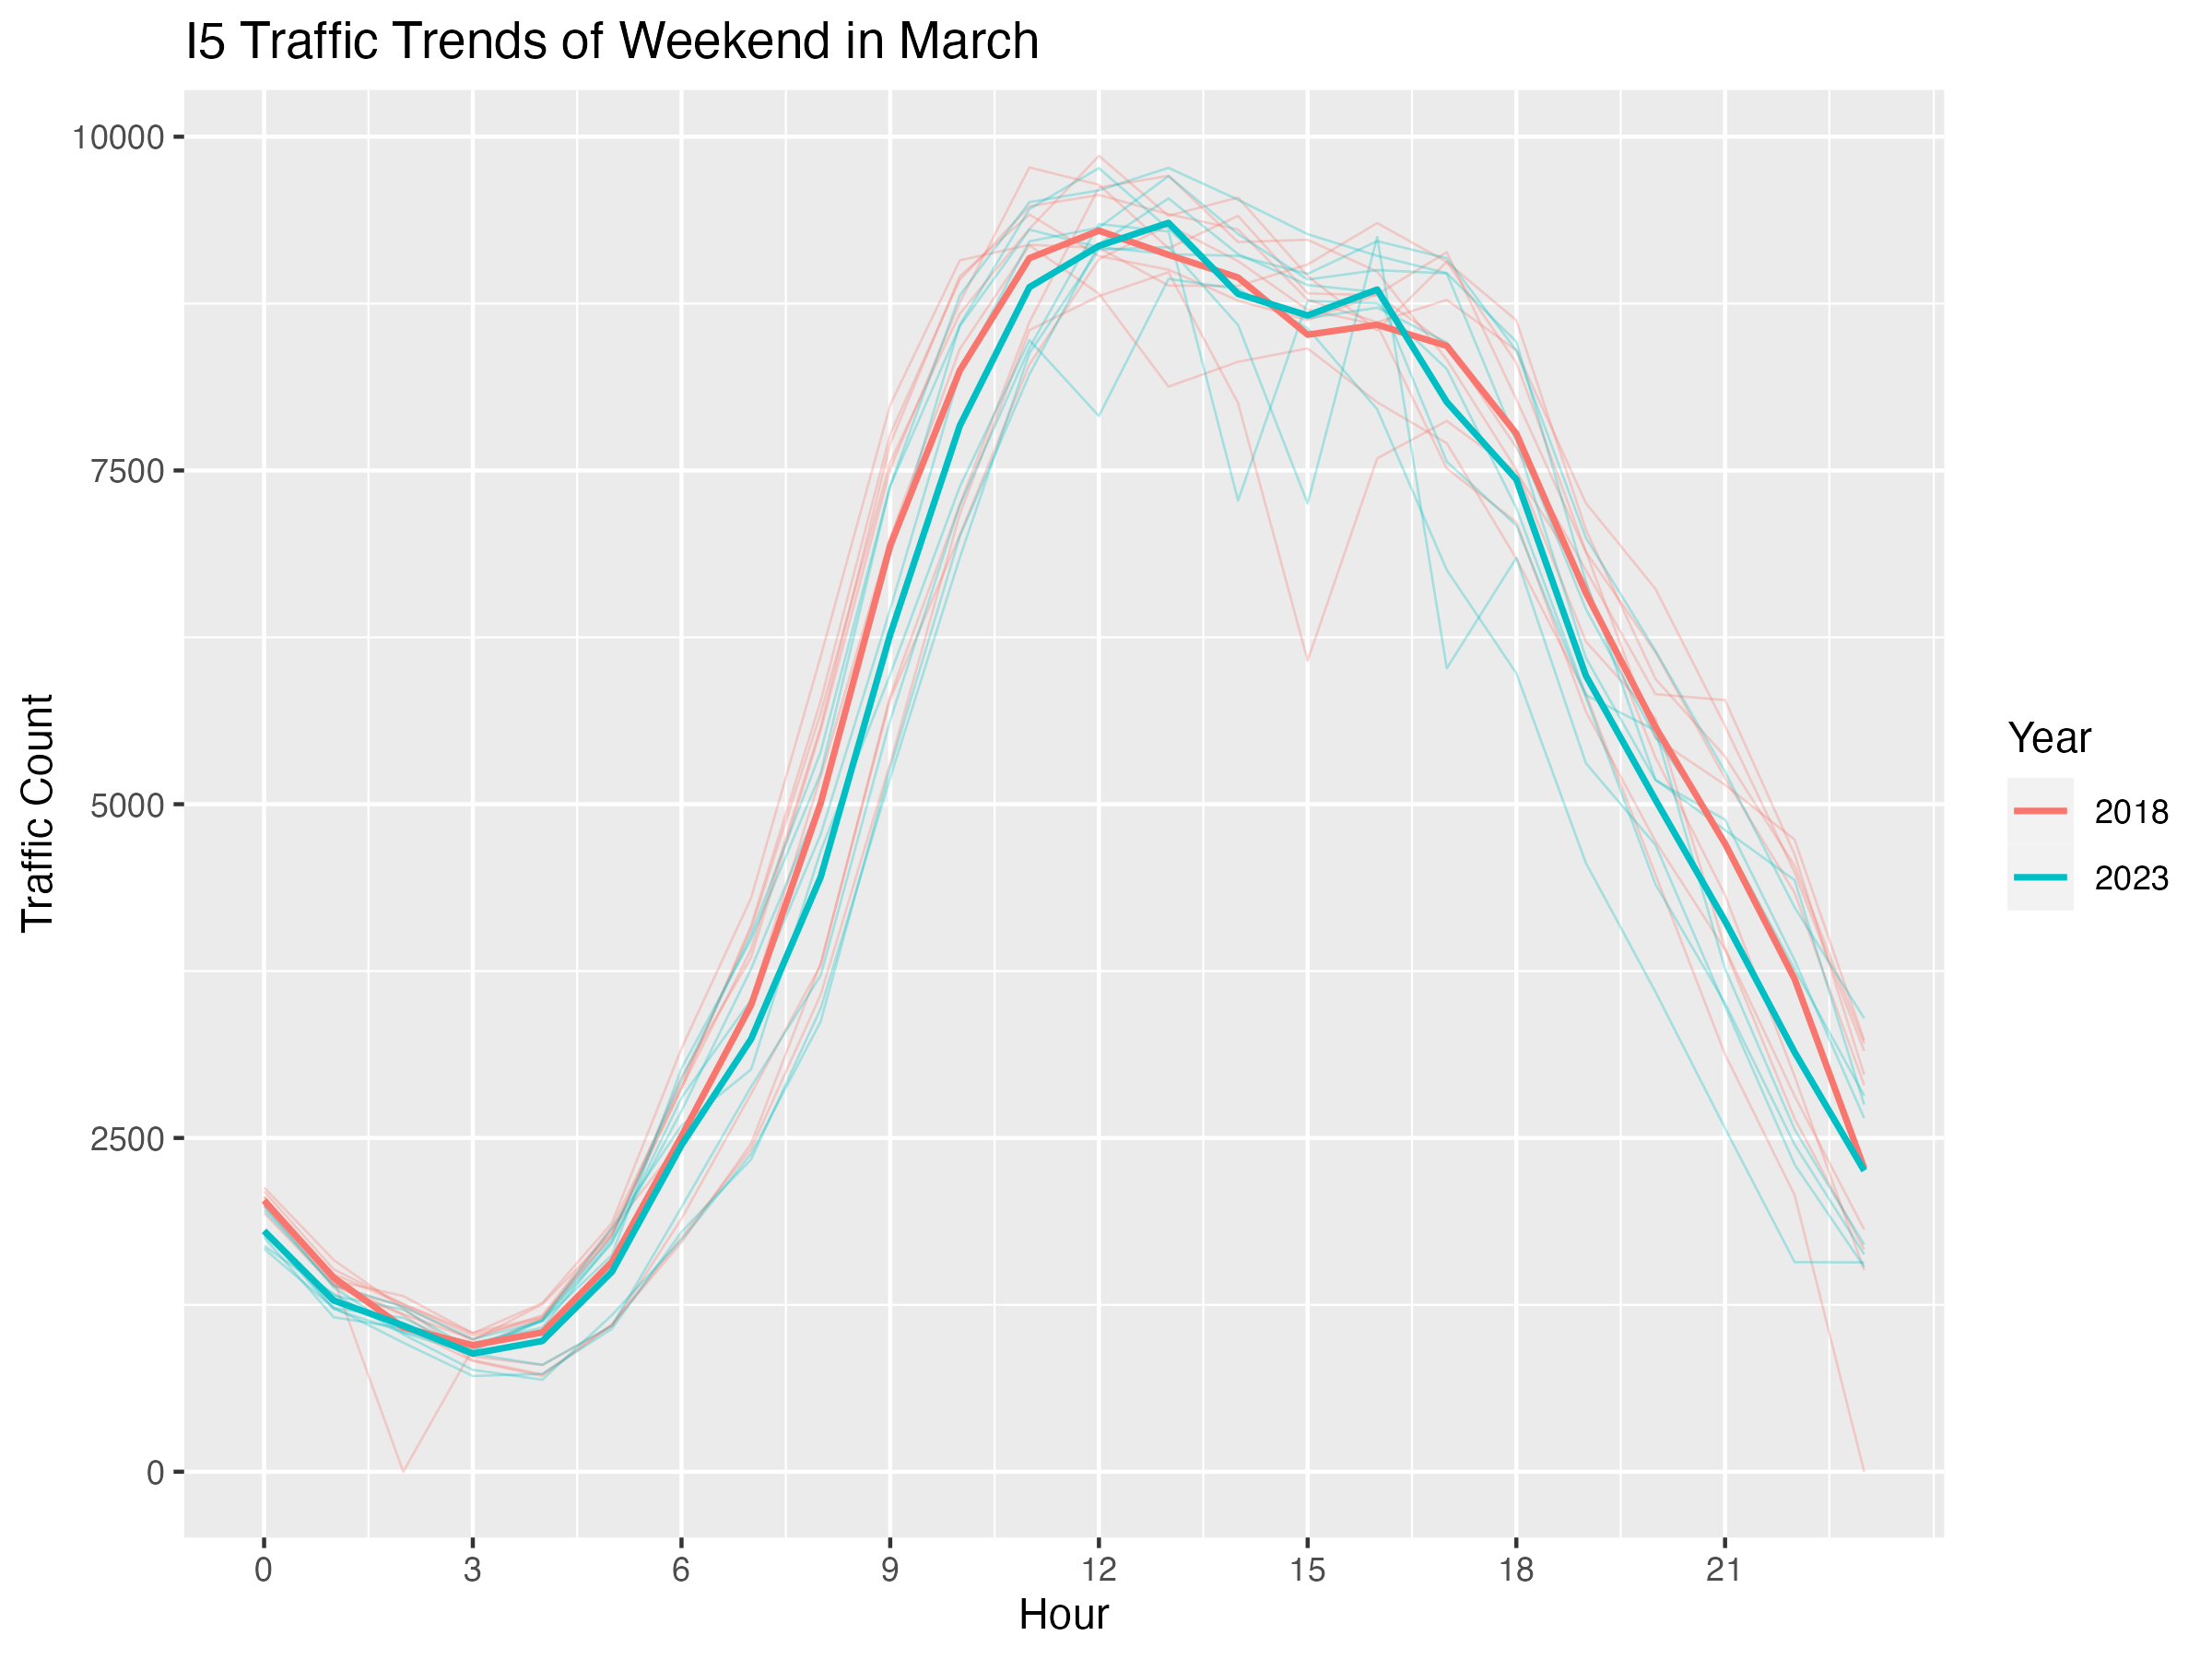
\includegraphics[width=\textwidth]{ATR26004_Plots/picture17_A04.png}
	\end{subfigure}
\end{figure}

\begin{figure}[H]
	\centering
	\begin{subfigure}[b]{0.45\textwidth}
		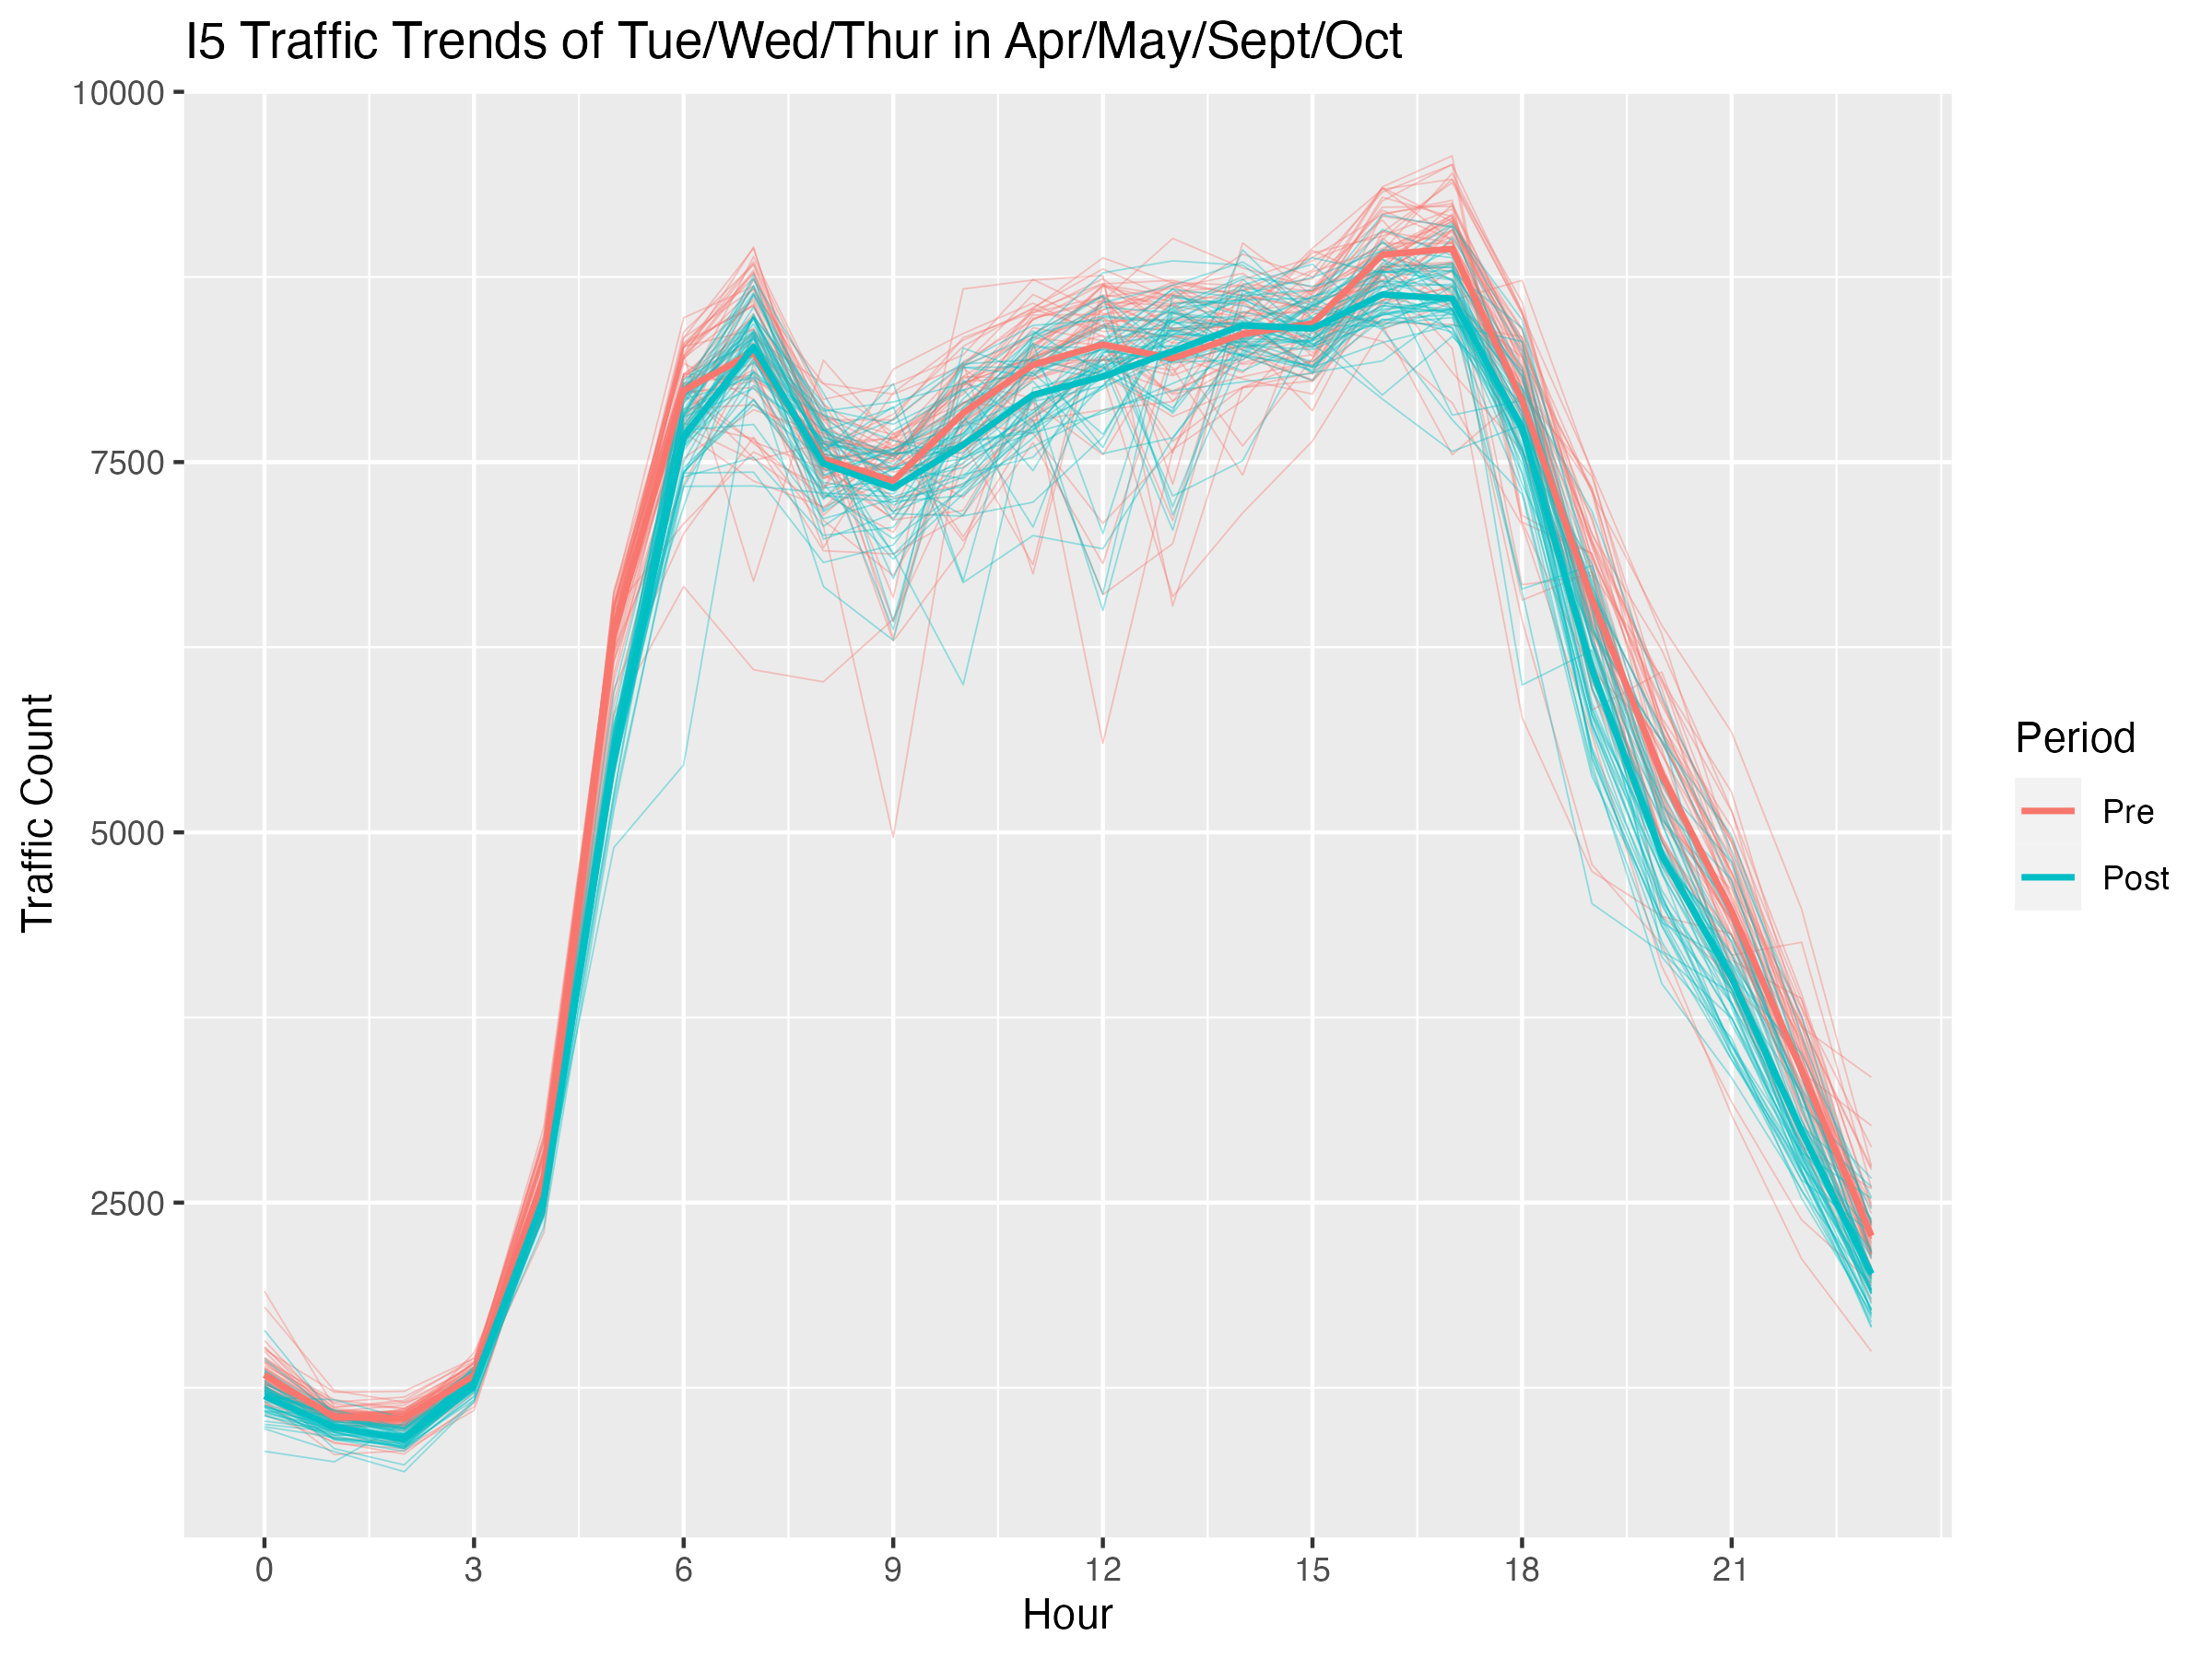
\includegraphics[width=\textwidth]{ATR26004_Plots/picture8_A04.png}
	\end{subfigure}
	\hfill
	\begin{subfigure}[b]{0.45\textwidth}
		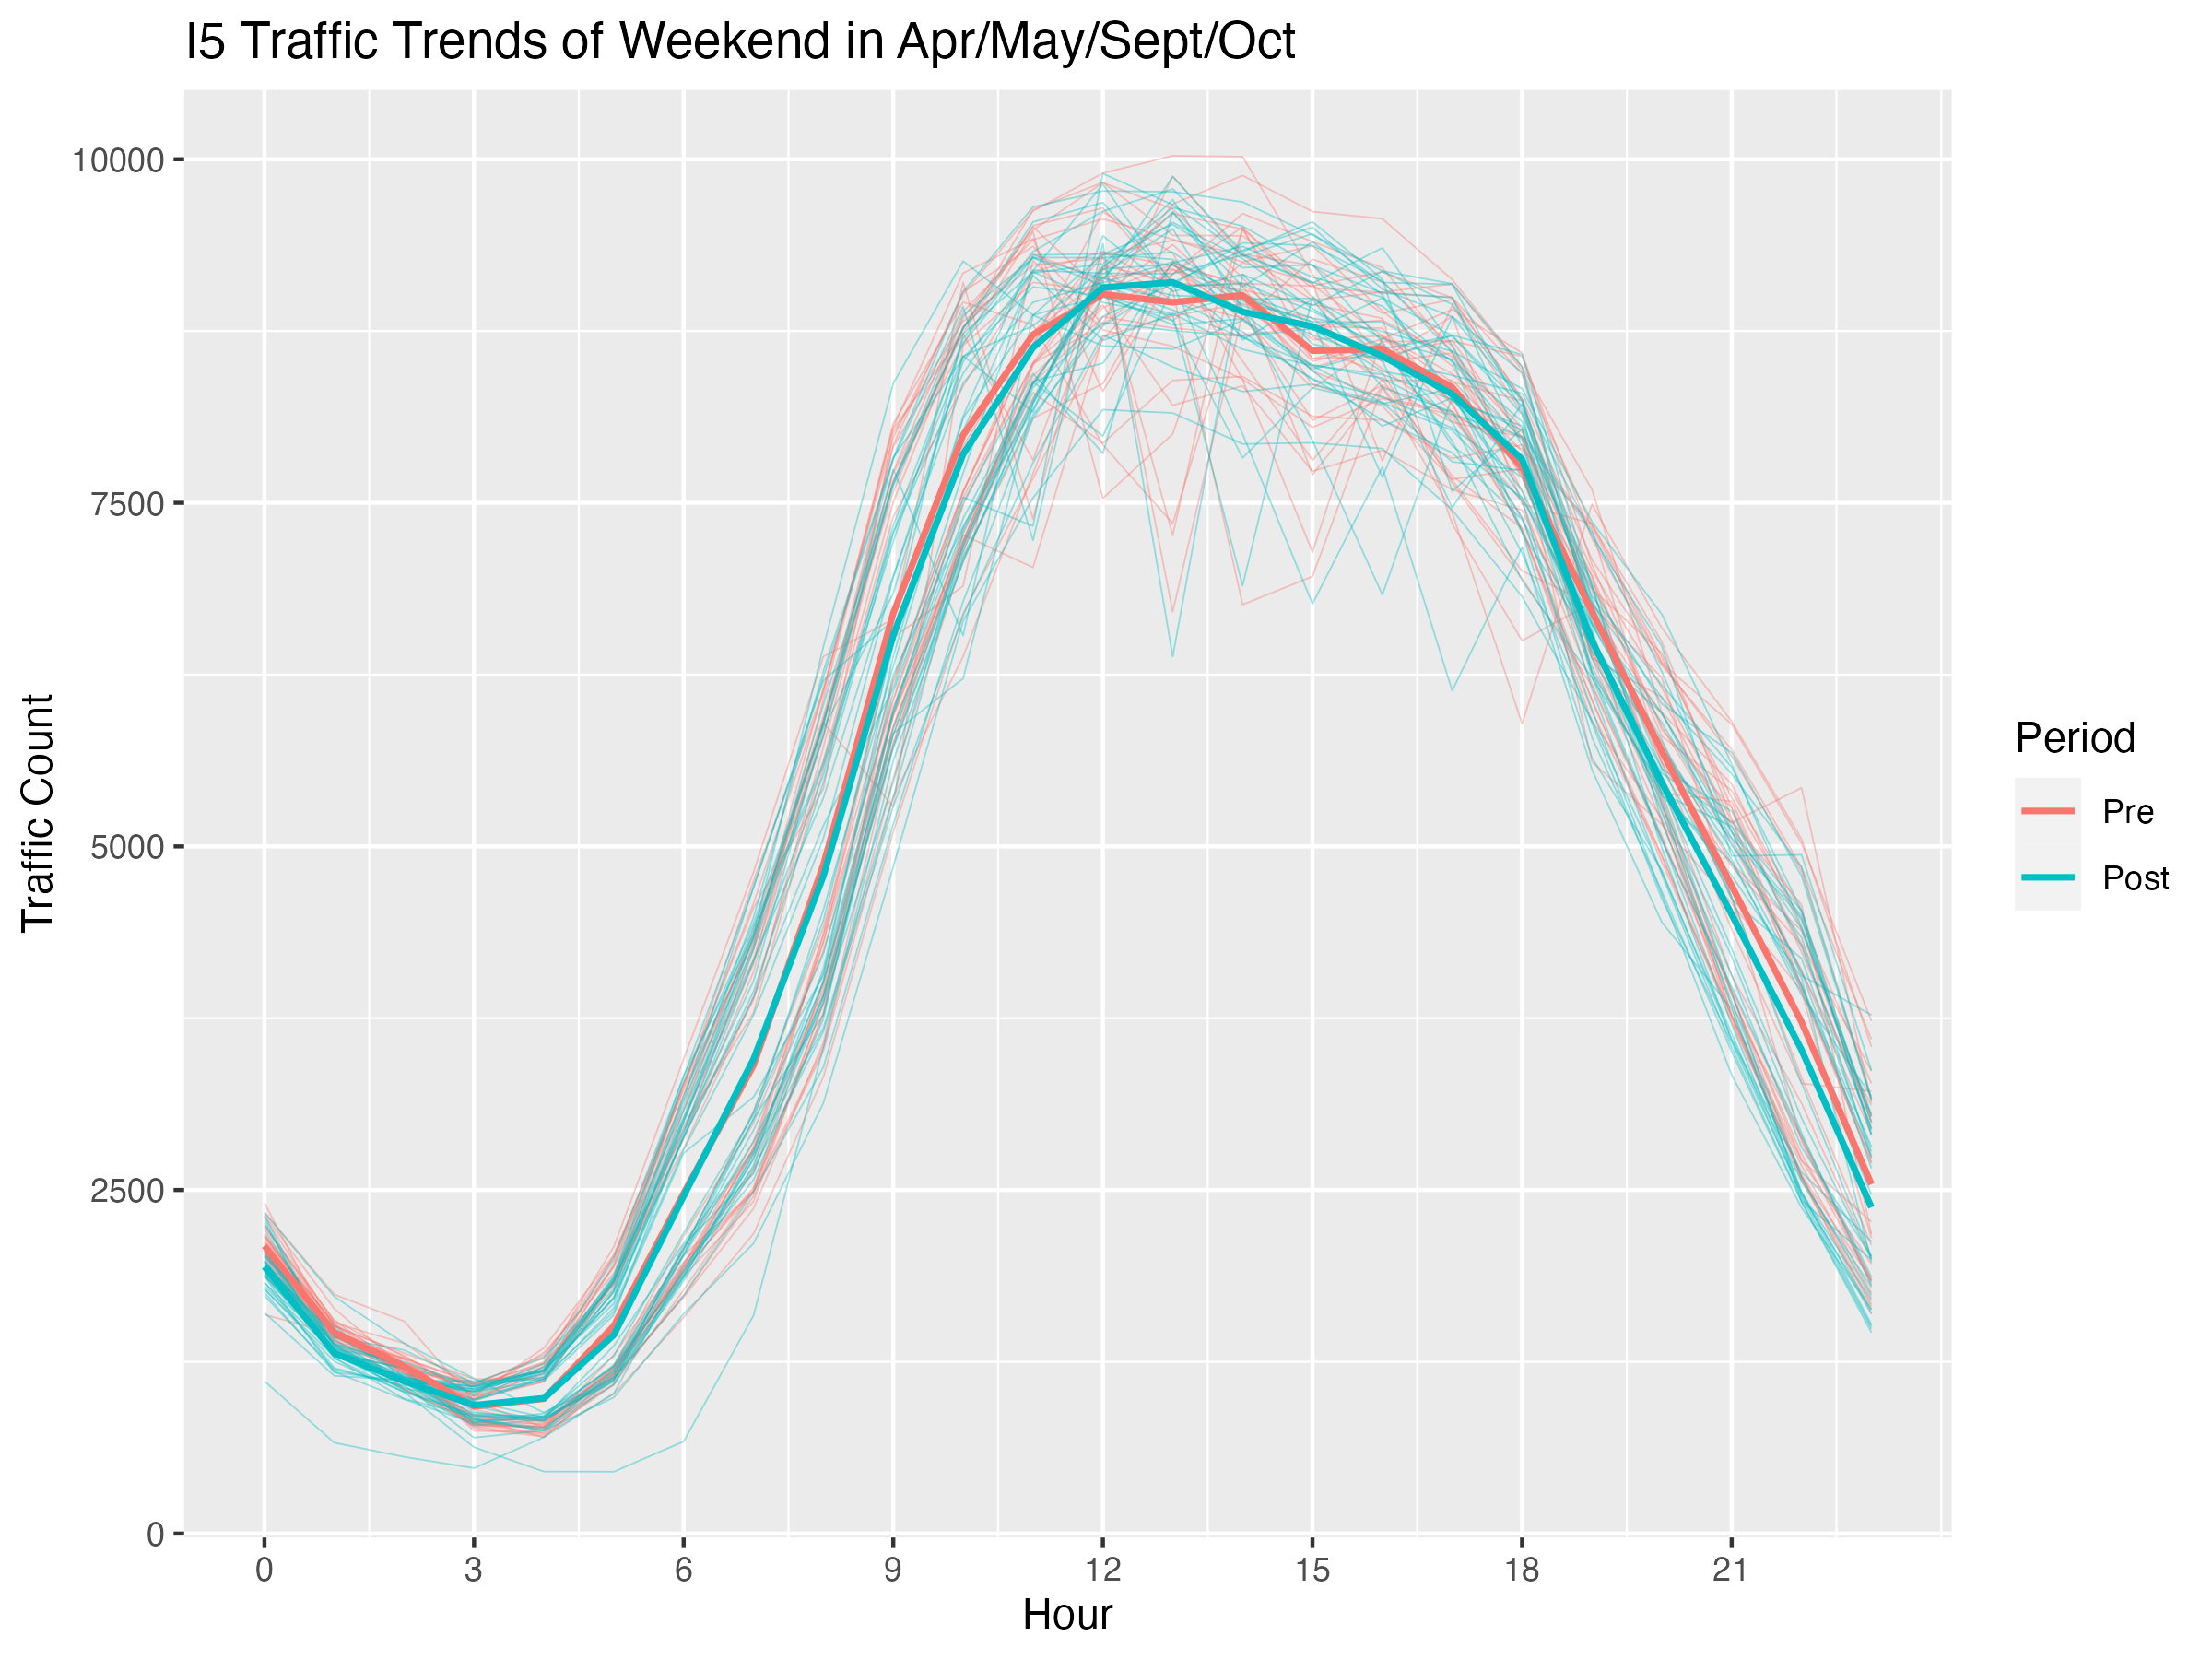
\includegraphics[width=\textwidth]{ATR26004_Plots/picture18_A04.png}
	\end{subfigure}
\end{figure}

\begin{figure}[H]
	\centering
	\begin{subfigure}[b]{0.45\textwidth}
		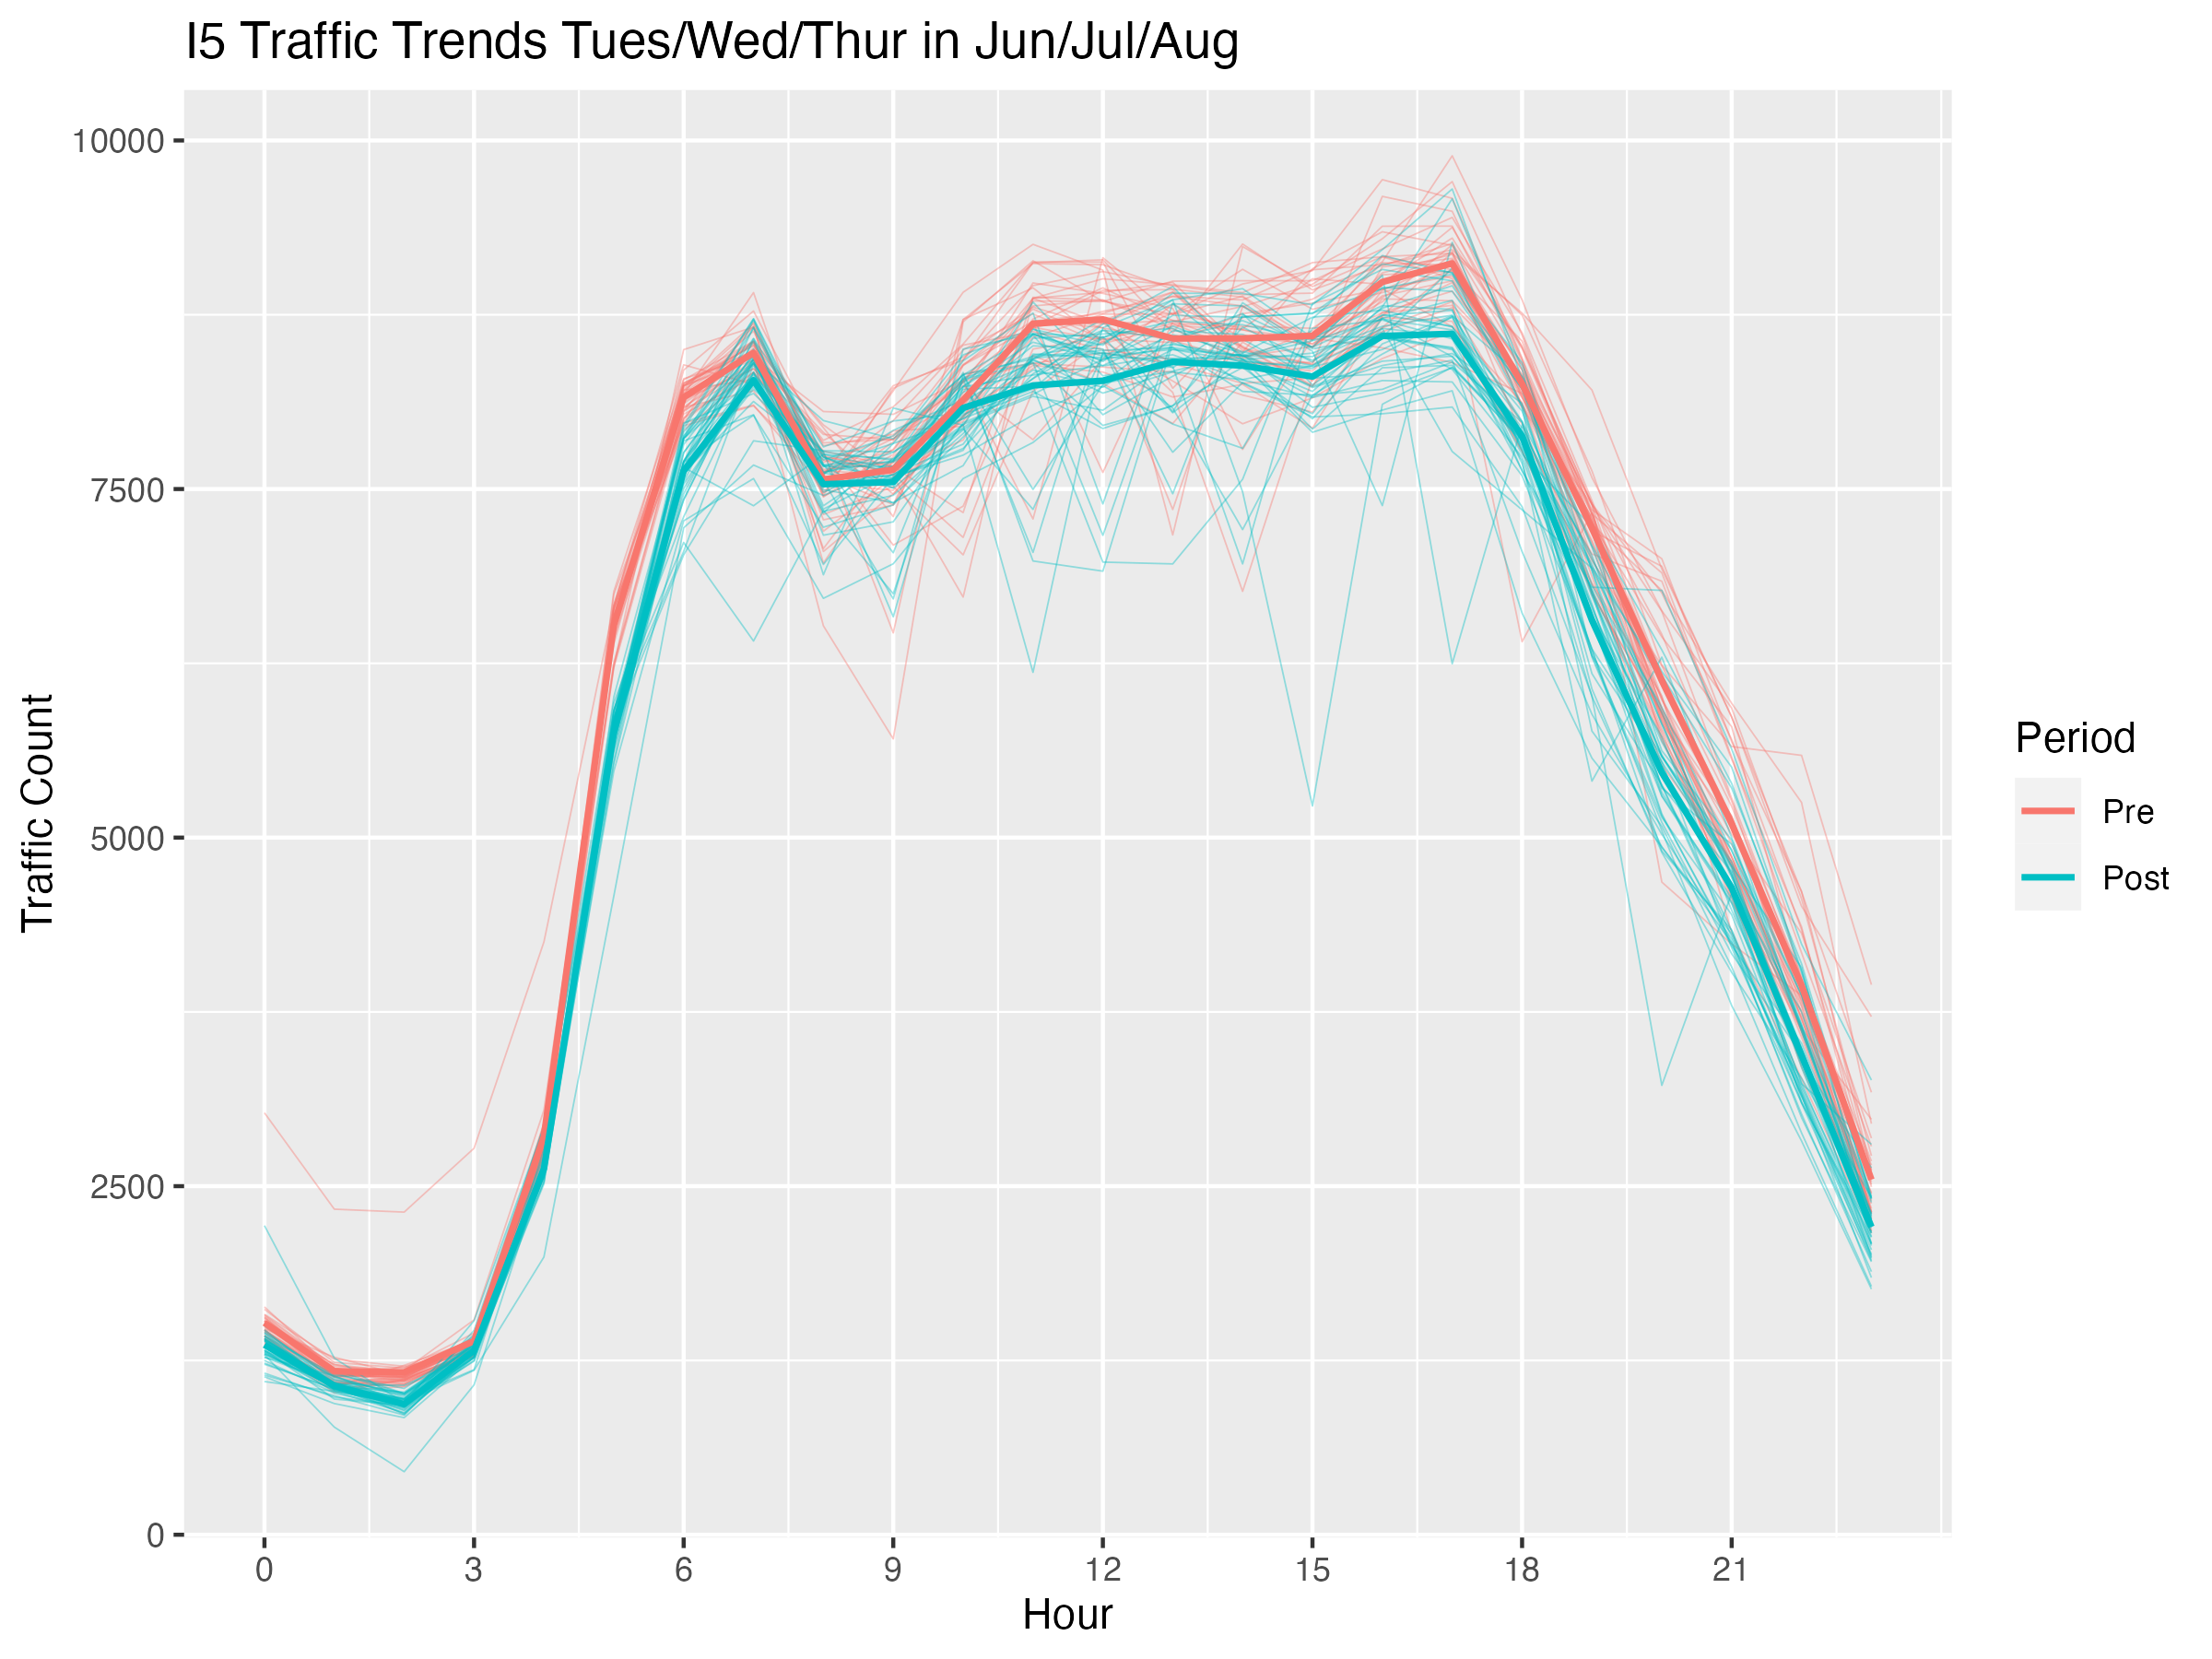
\includegraphics[width=\textwidth]{ATR26004_Plots/picture9_A04.png}
	\end{subfigure}
	\hfill
	\begin{subfigure}[b]{0.45\textwidth}
		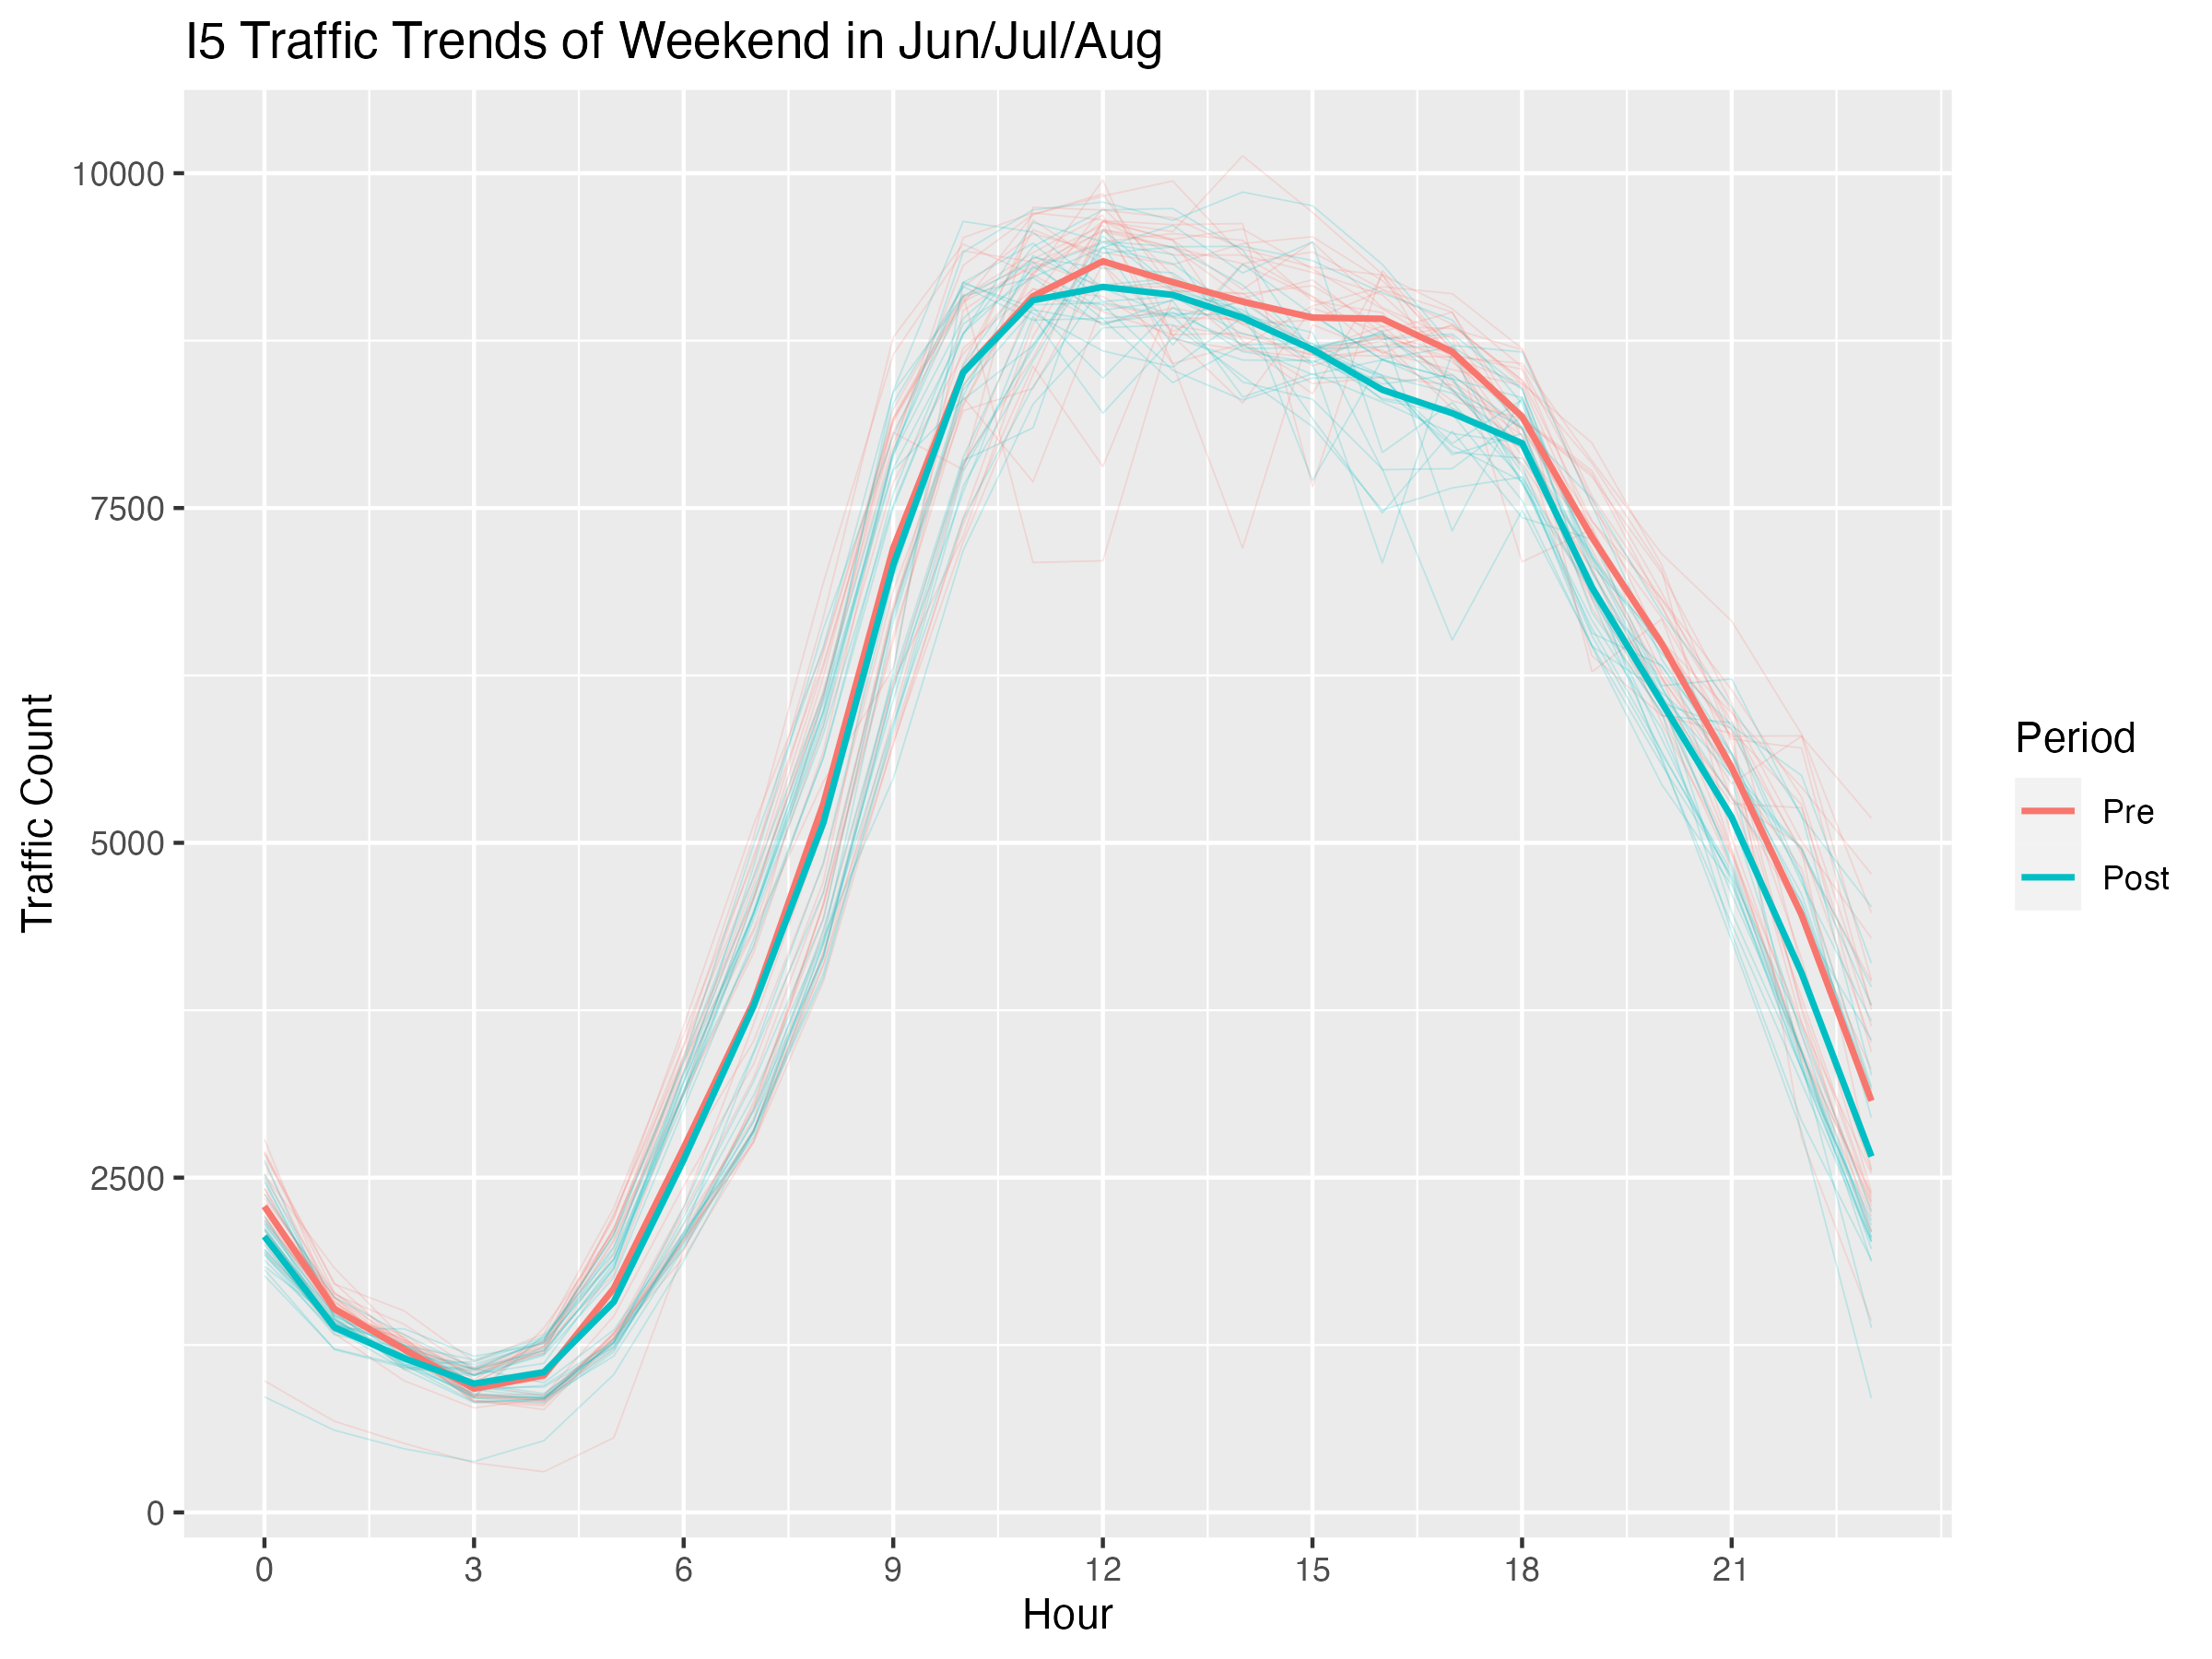
\includegraphics[width=\textwidth]{ATR26004_Plots/picture19_A04.png}
	\end{subfigure}
\end{figure}

\begin{figure}[H]
	\centering
	\begin{subfigure}[b]{0.45\textwidth}
		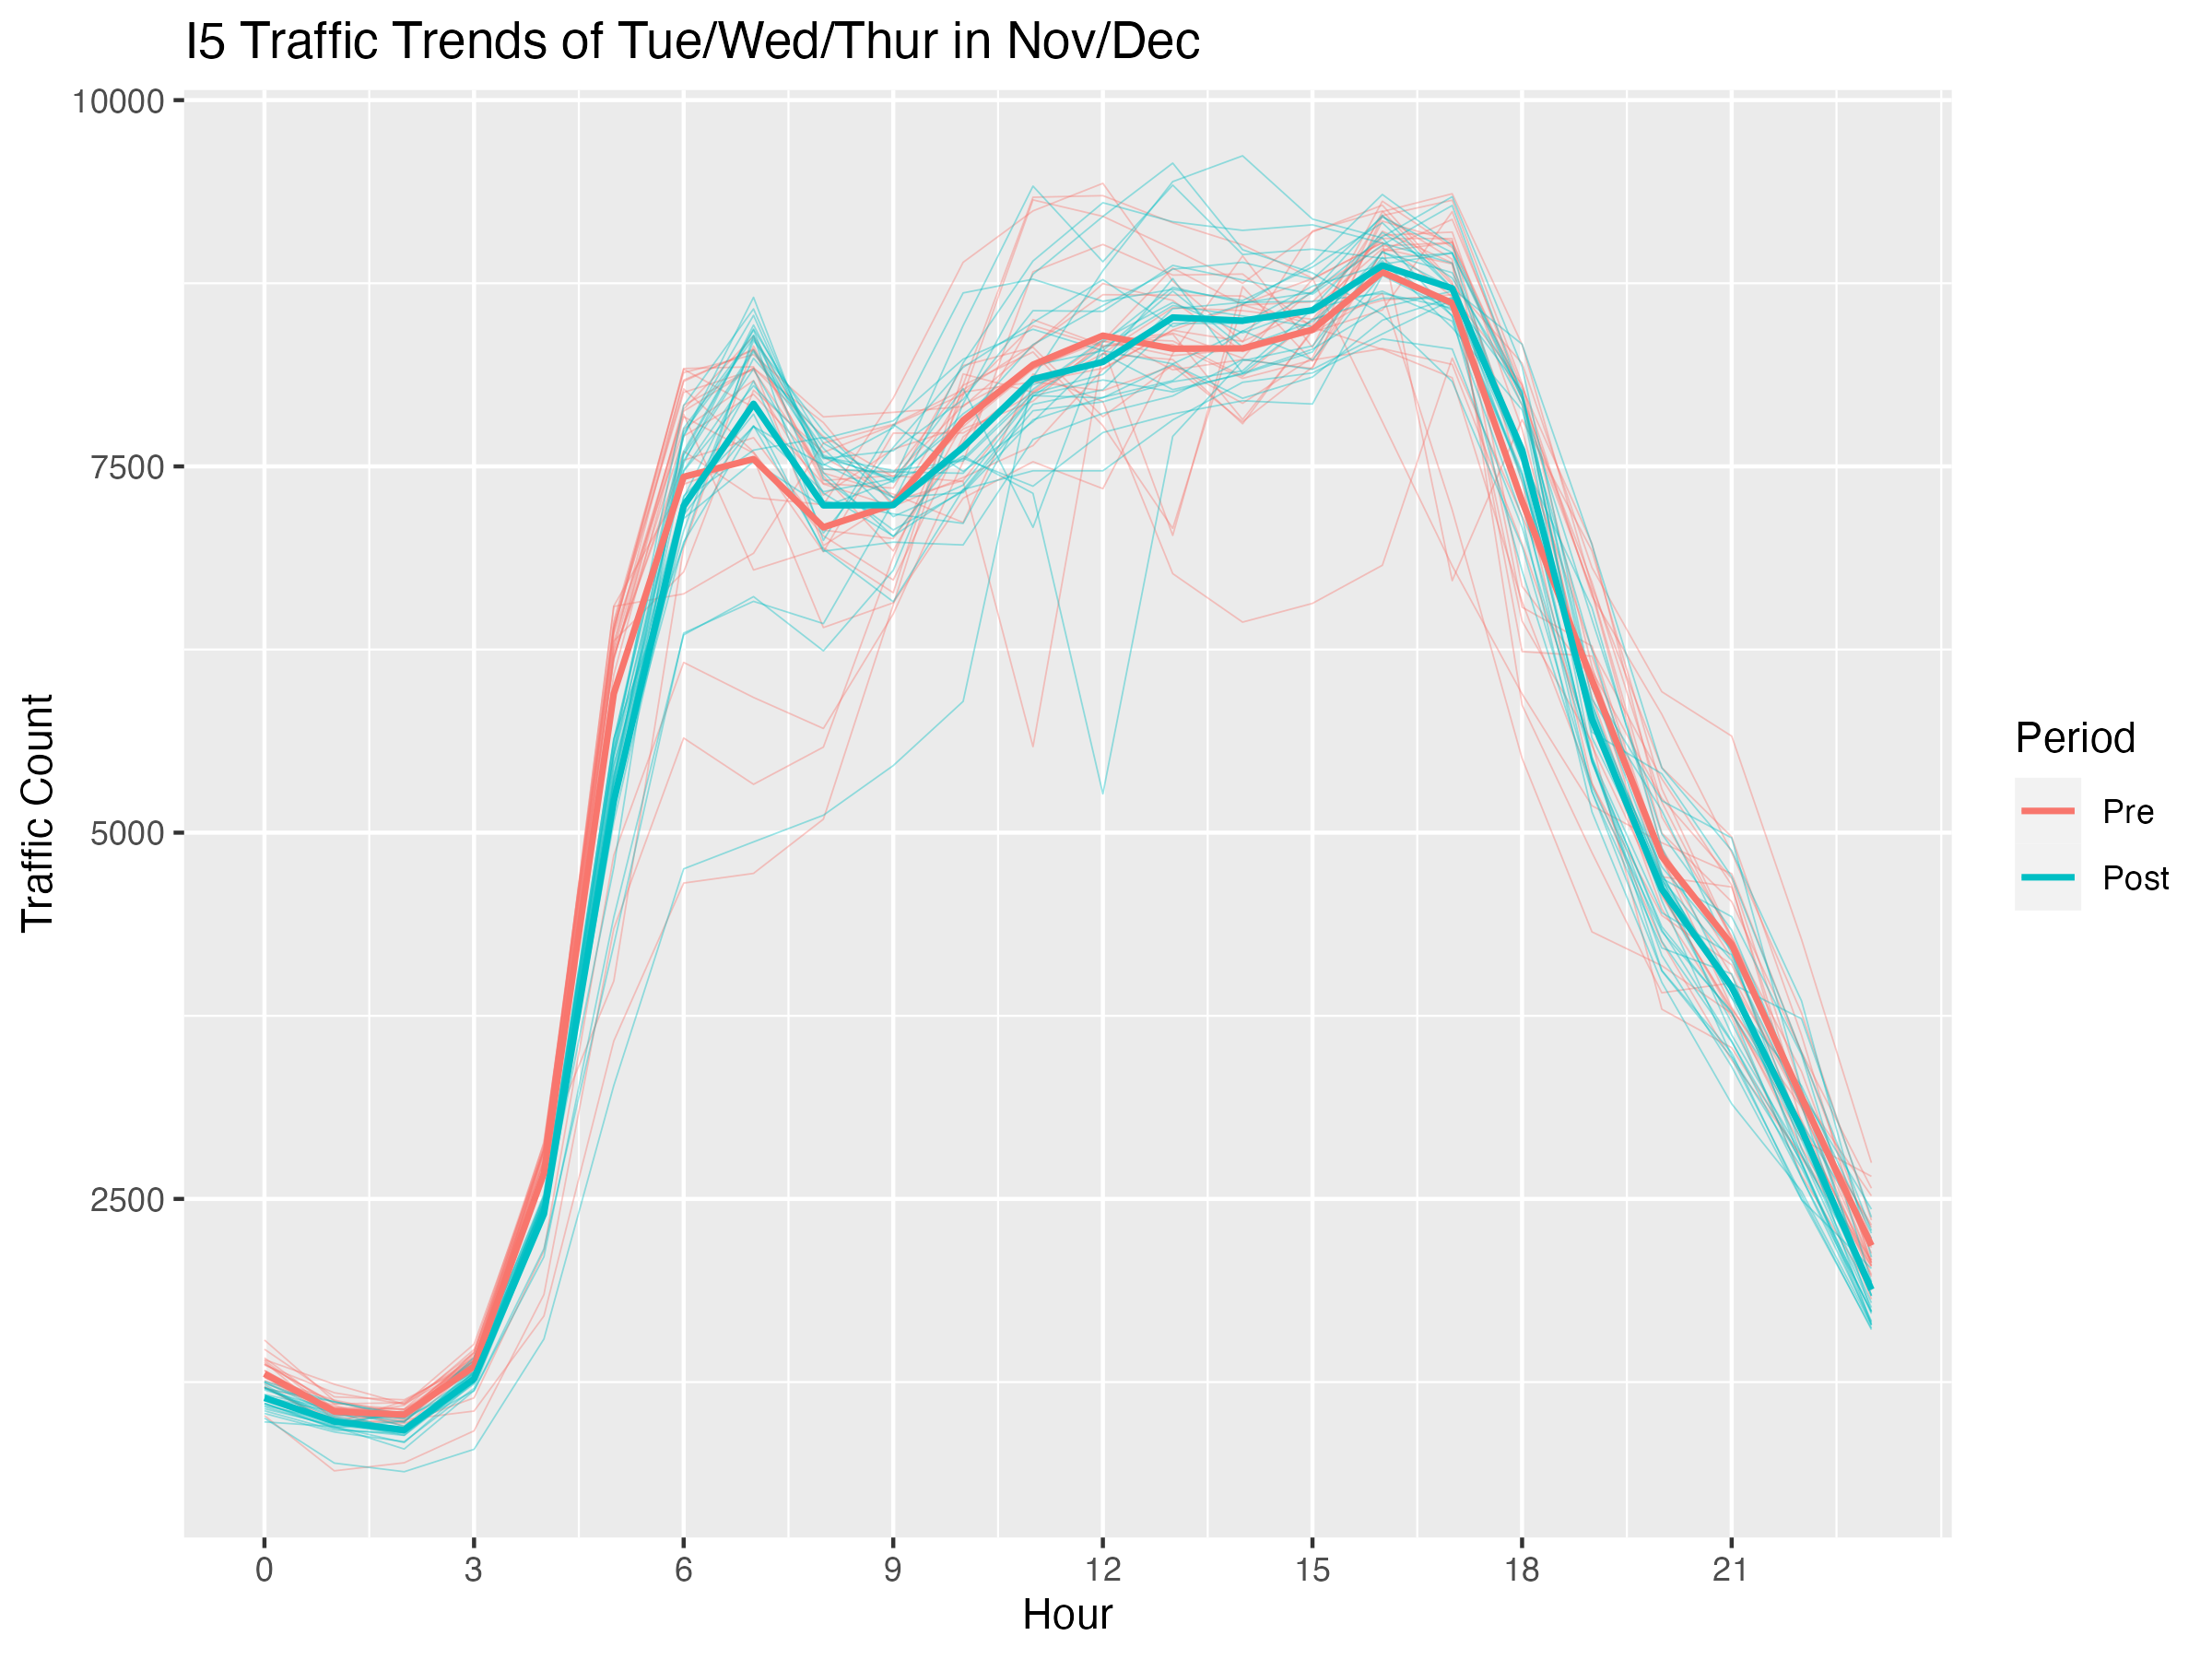
\includegraphics[width=\textwidth]{ATR26004_Plots/picture10_A04.png}
	\end{subfigure}
	\hfill
	\begin{subfigure}[b]{0.45\textwidth}
		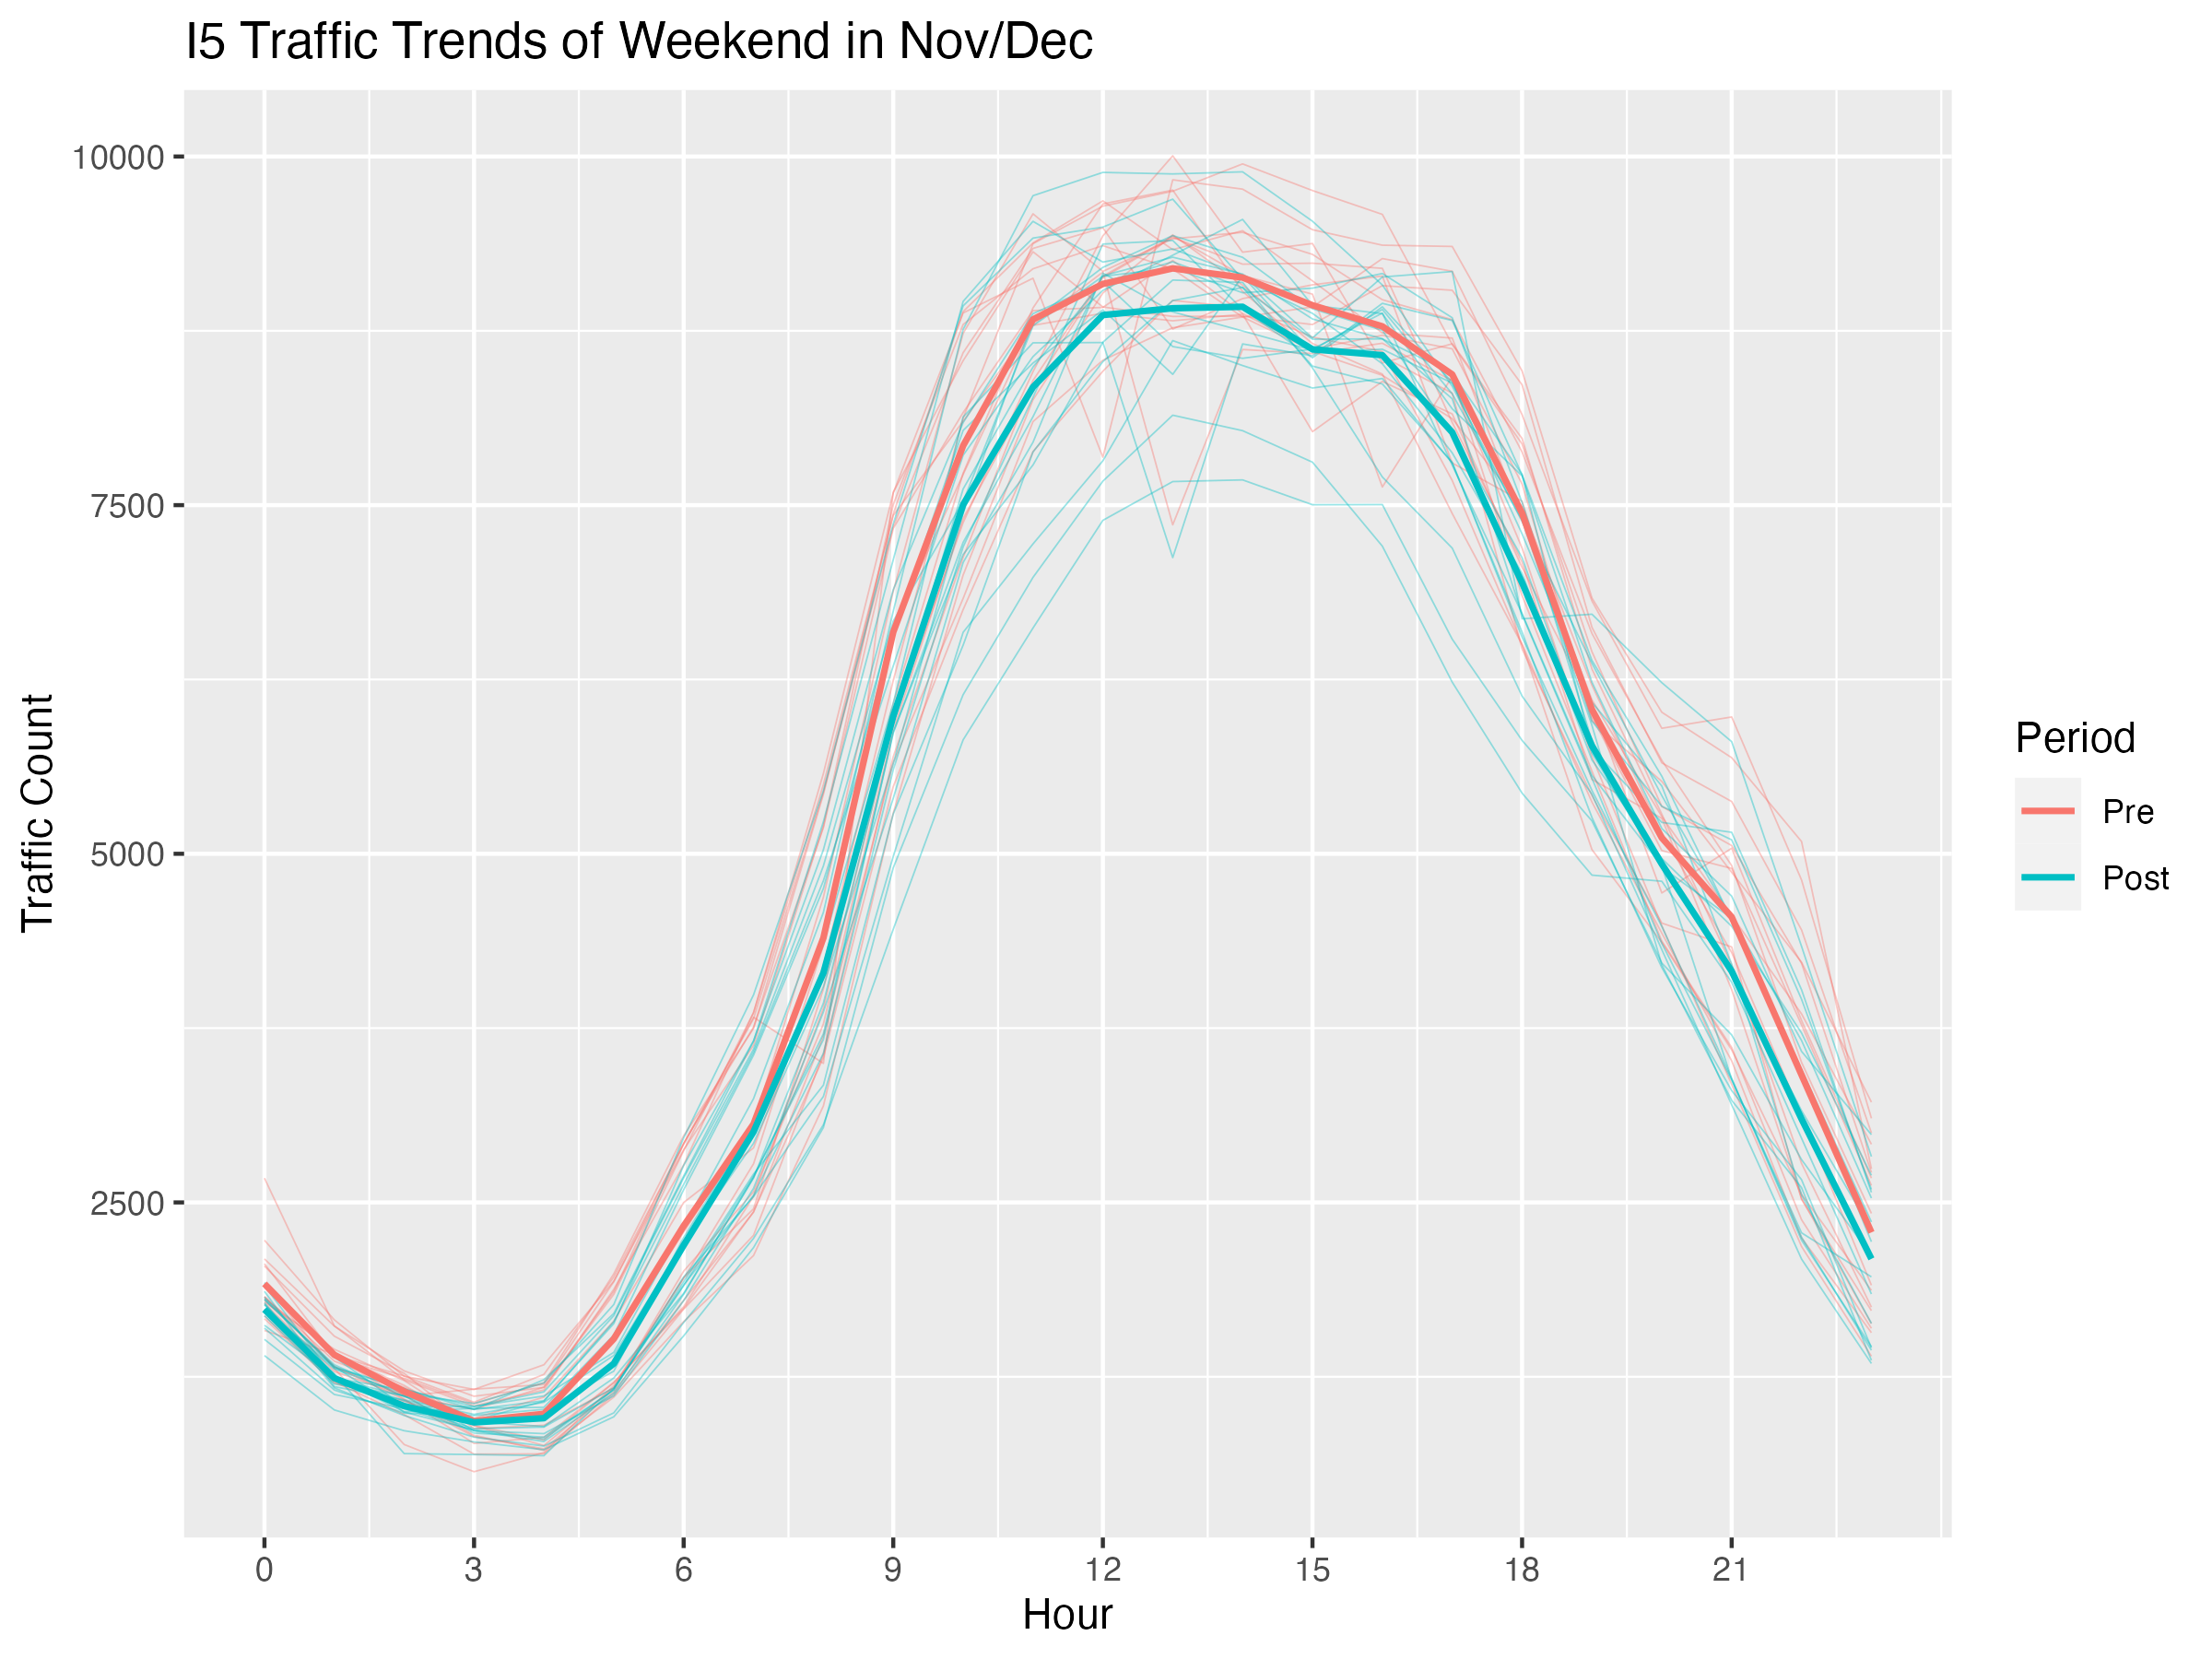
\includegraphics[width=\textwidth]{ATR26004_Plots/picture20_A04.png}
	\end{subfigure}
\end{figure}

\begin{figure}[H]
	\centering
	\begin{subfigure}[b]{0.45\textwidth}
		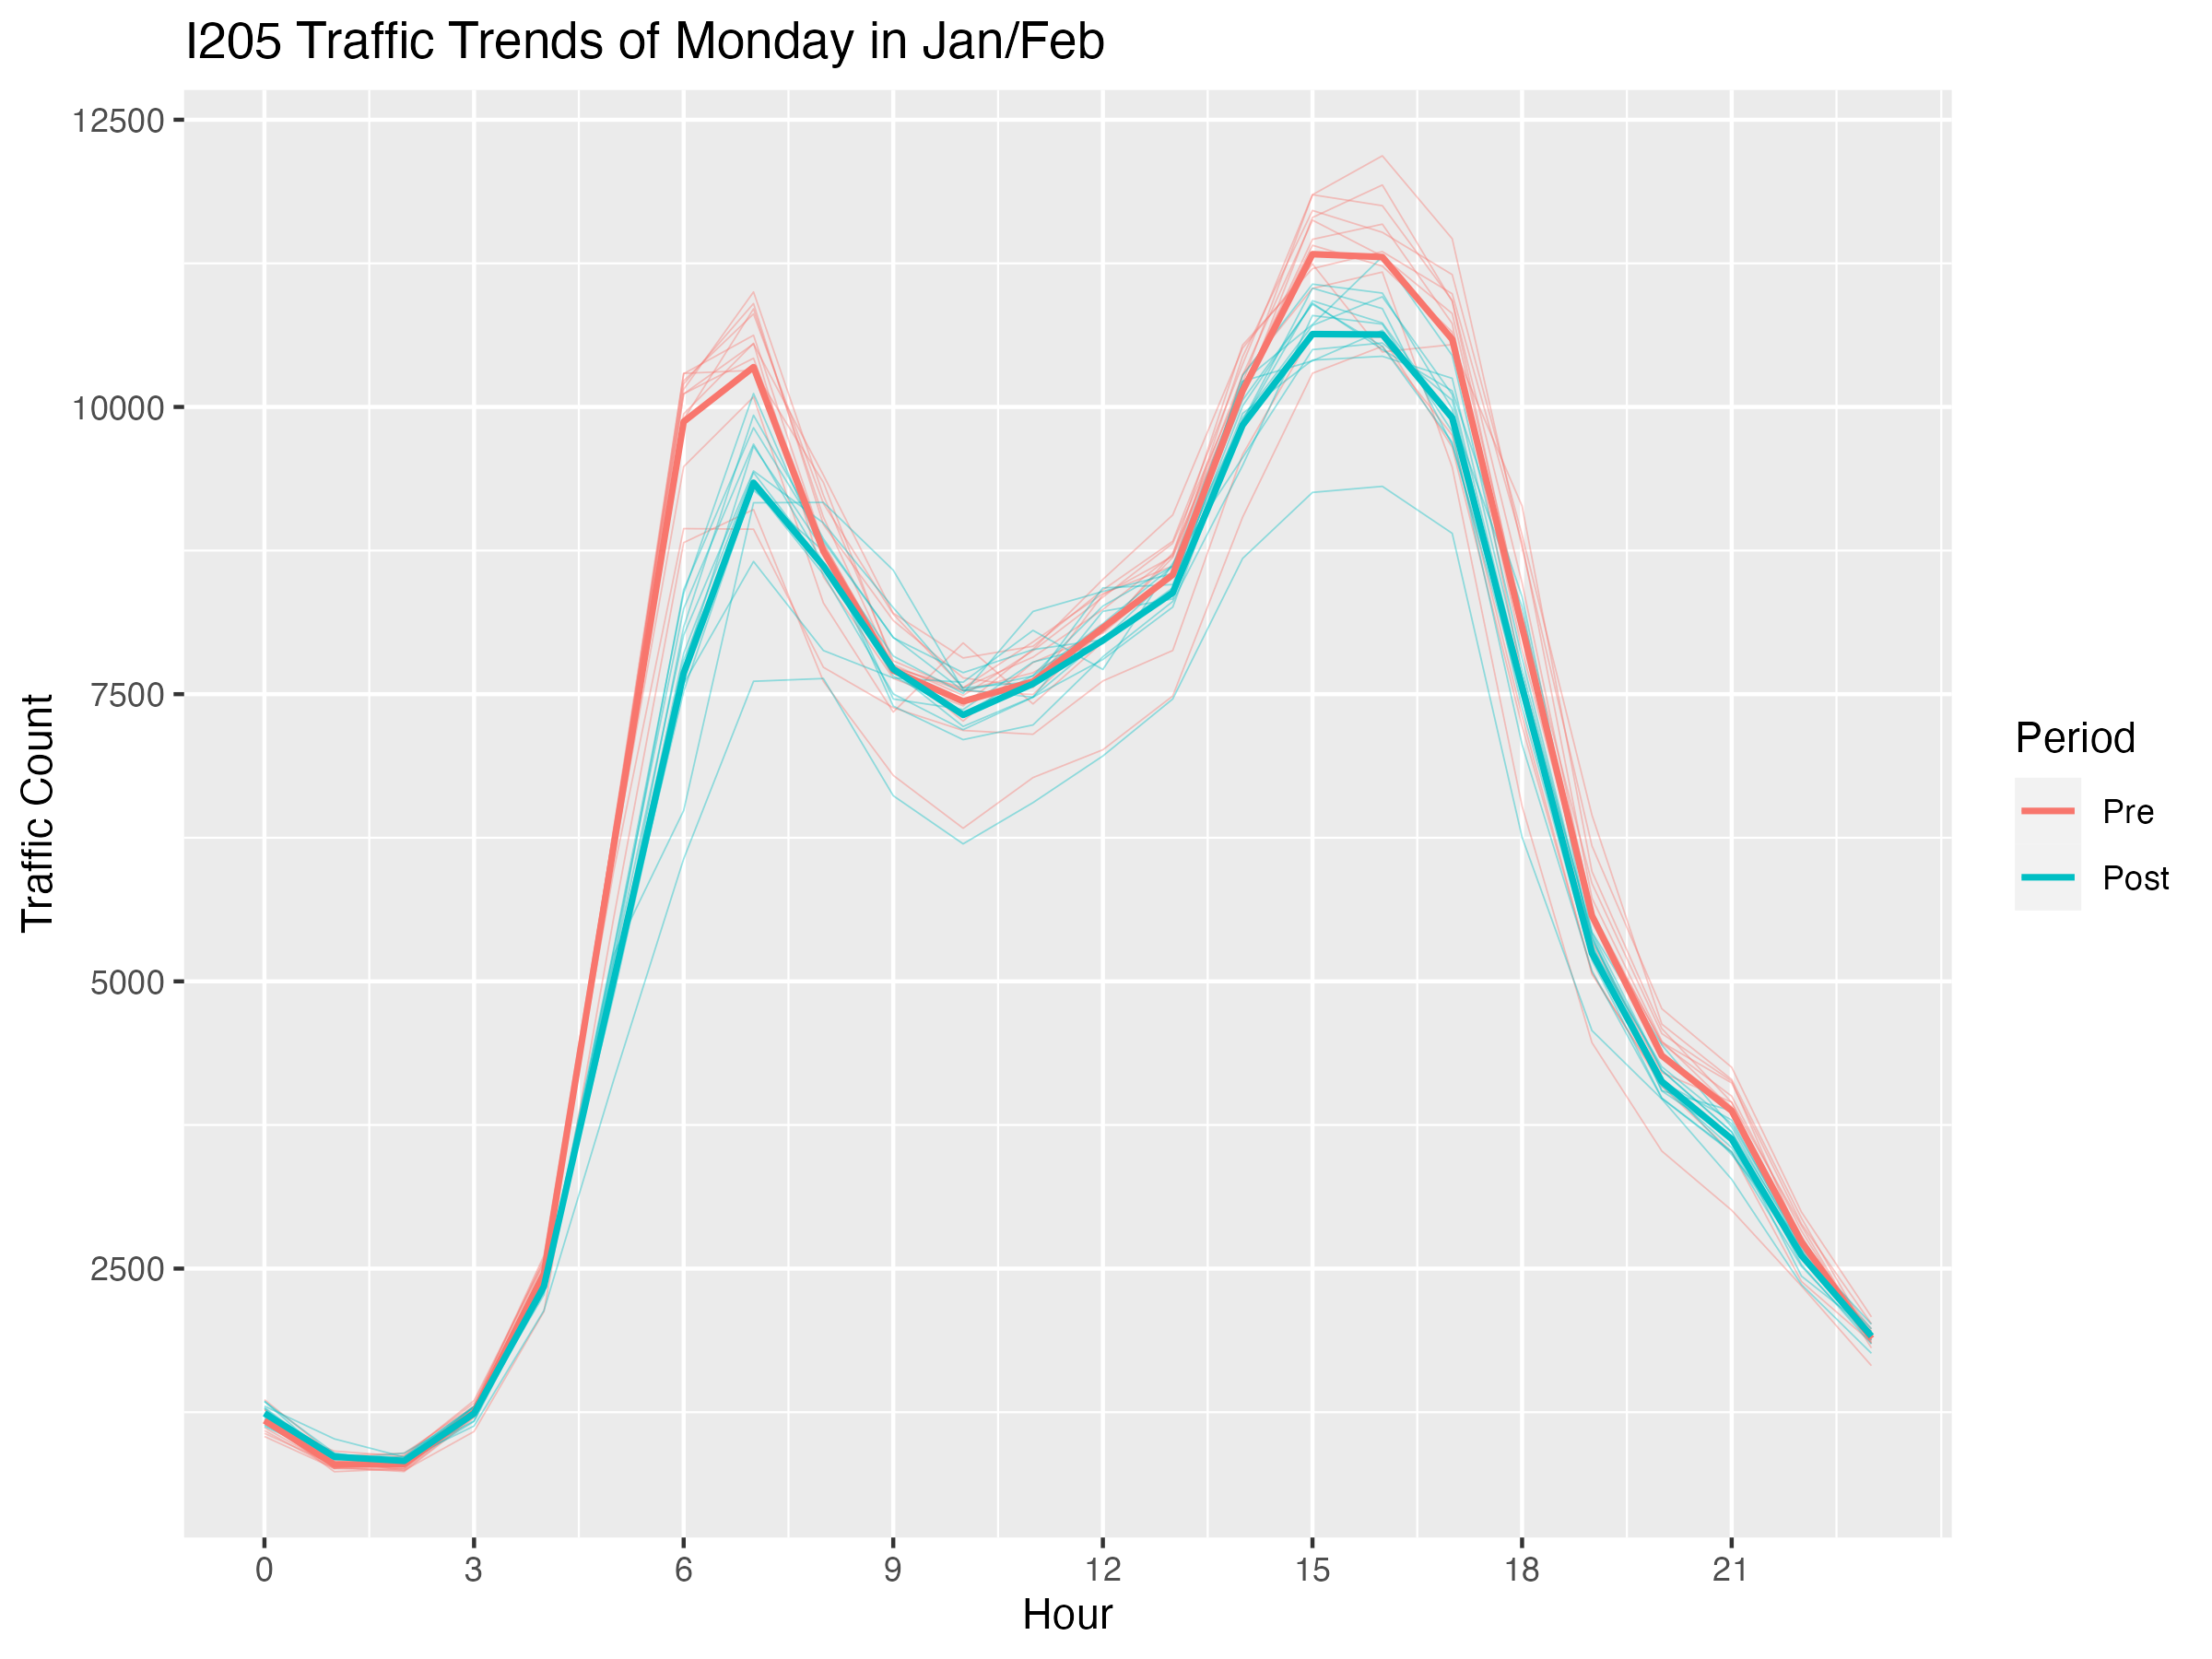
\includegraphics[width=\textwidth]{ATR26024_Plots/picture1_A24.png}
	\end{subfigure}
	\hfill
	\begin{subfigure}[b]{0.45\textwidth}
		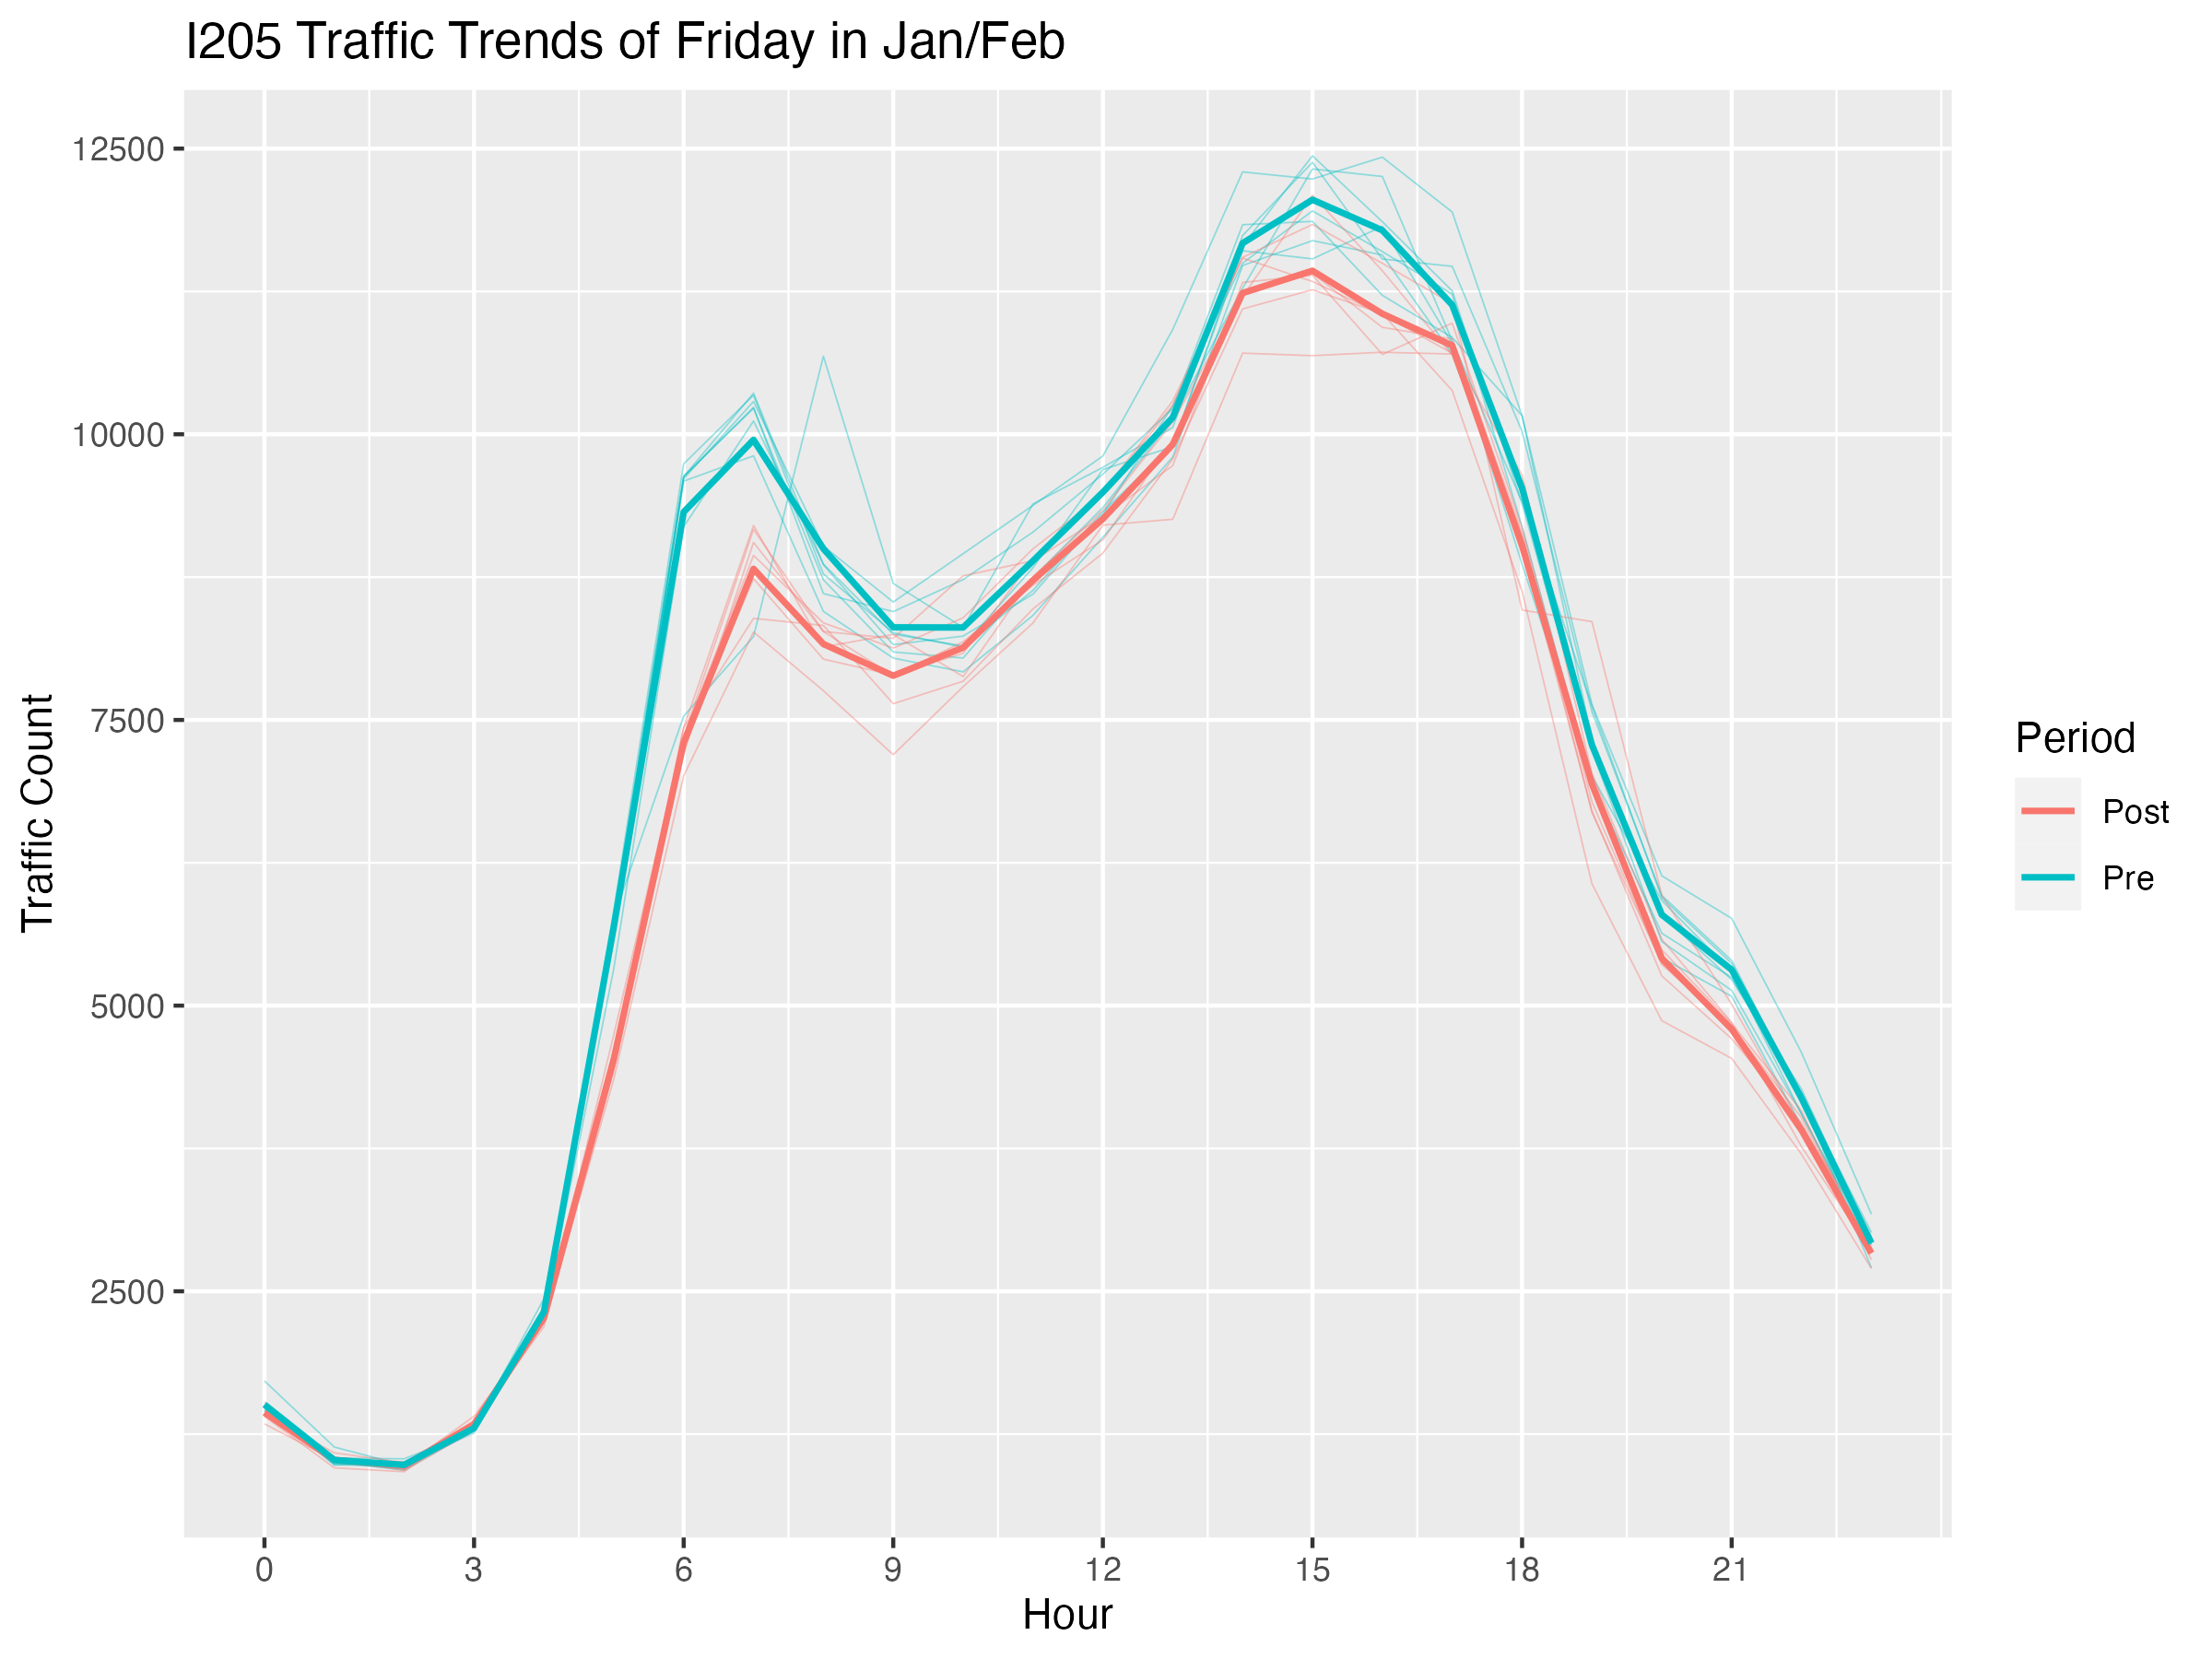
\includegraphics[width=\textwidth]{ATR26024_Plots/picture11_A24.png}
	\end{subfigure}
\end{figure}

\begin{figure}[H]
	\centering
	\begin{subfigure}[b]{0.45\textwidth}
		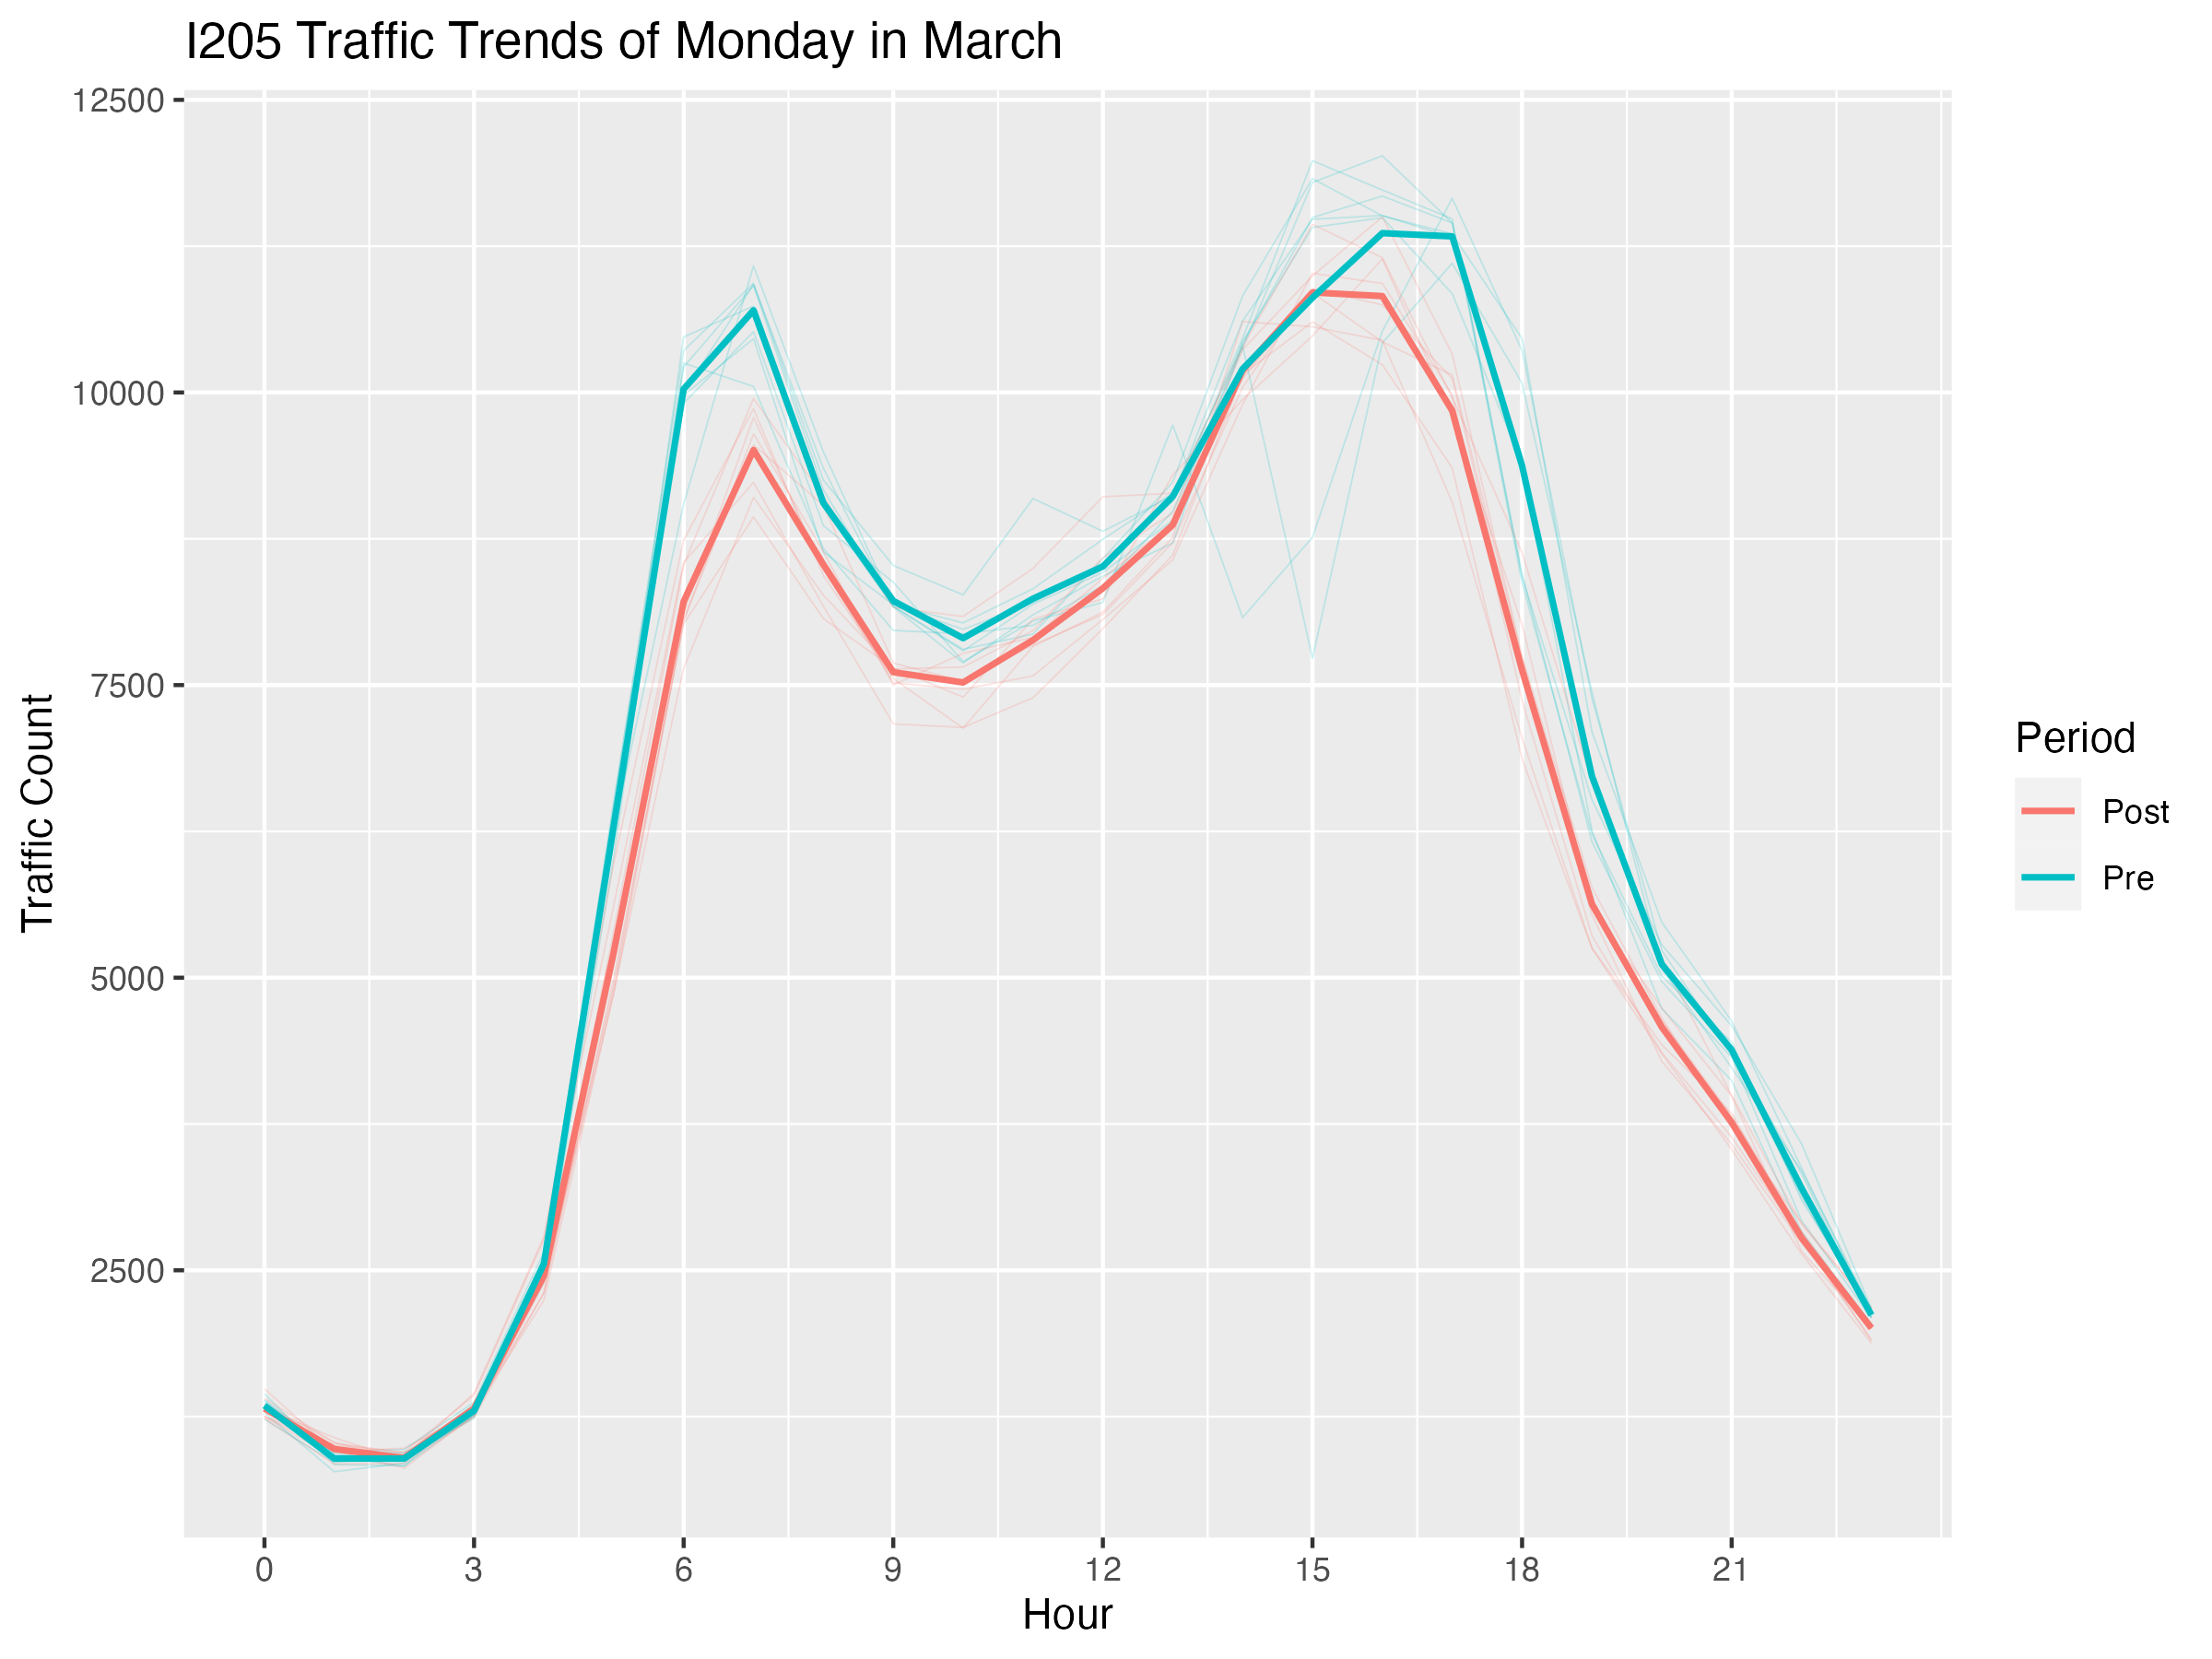
\includegraphics[width=\textwidth]{ATR26024_Plots/picture2_A24.png}
	\end{subfigure}
	\hfill
	\begin{subfigure}[b]{0.45\textwidth}
		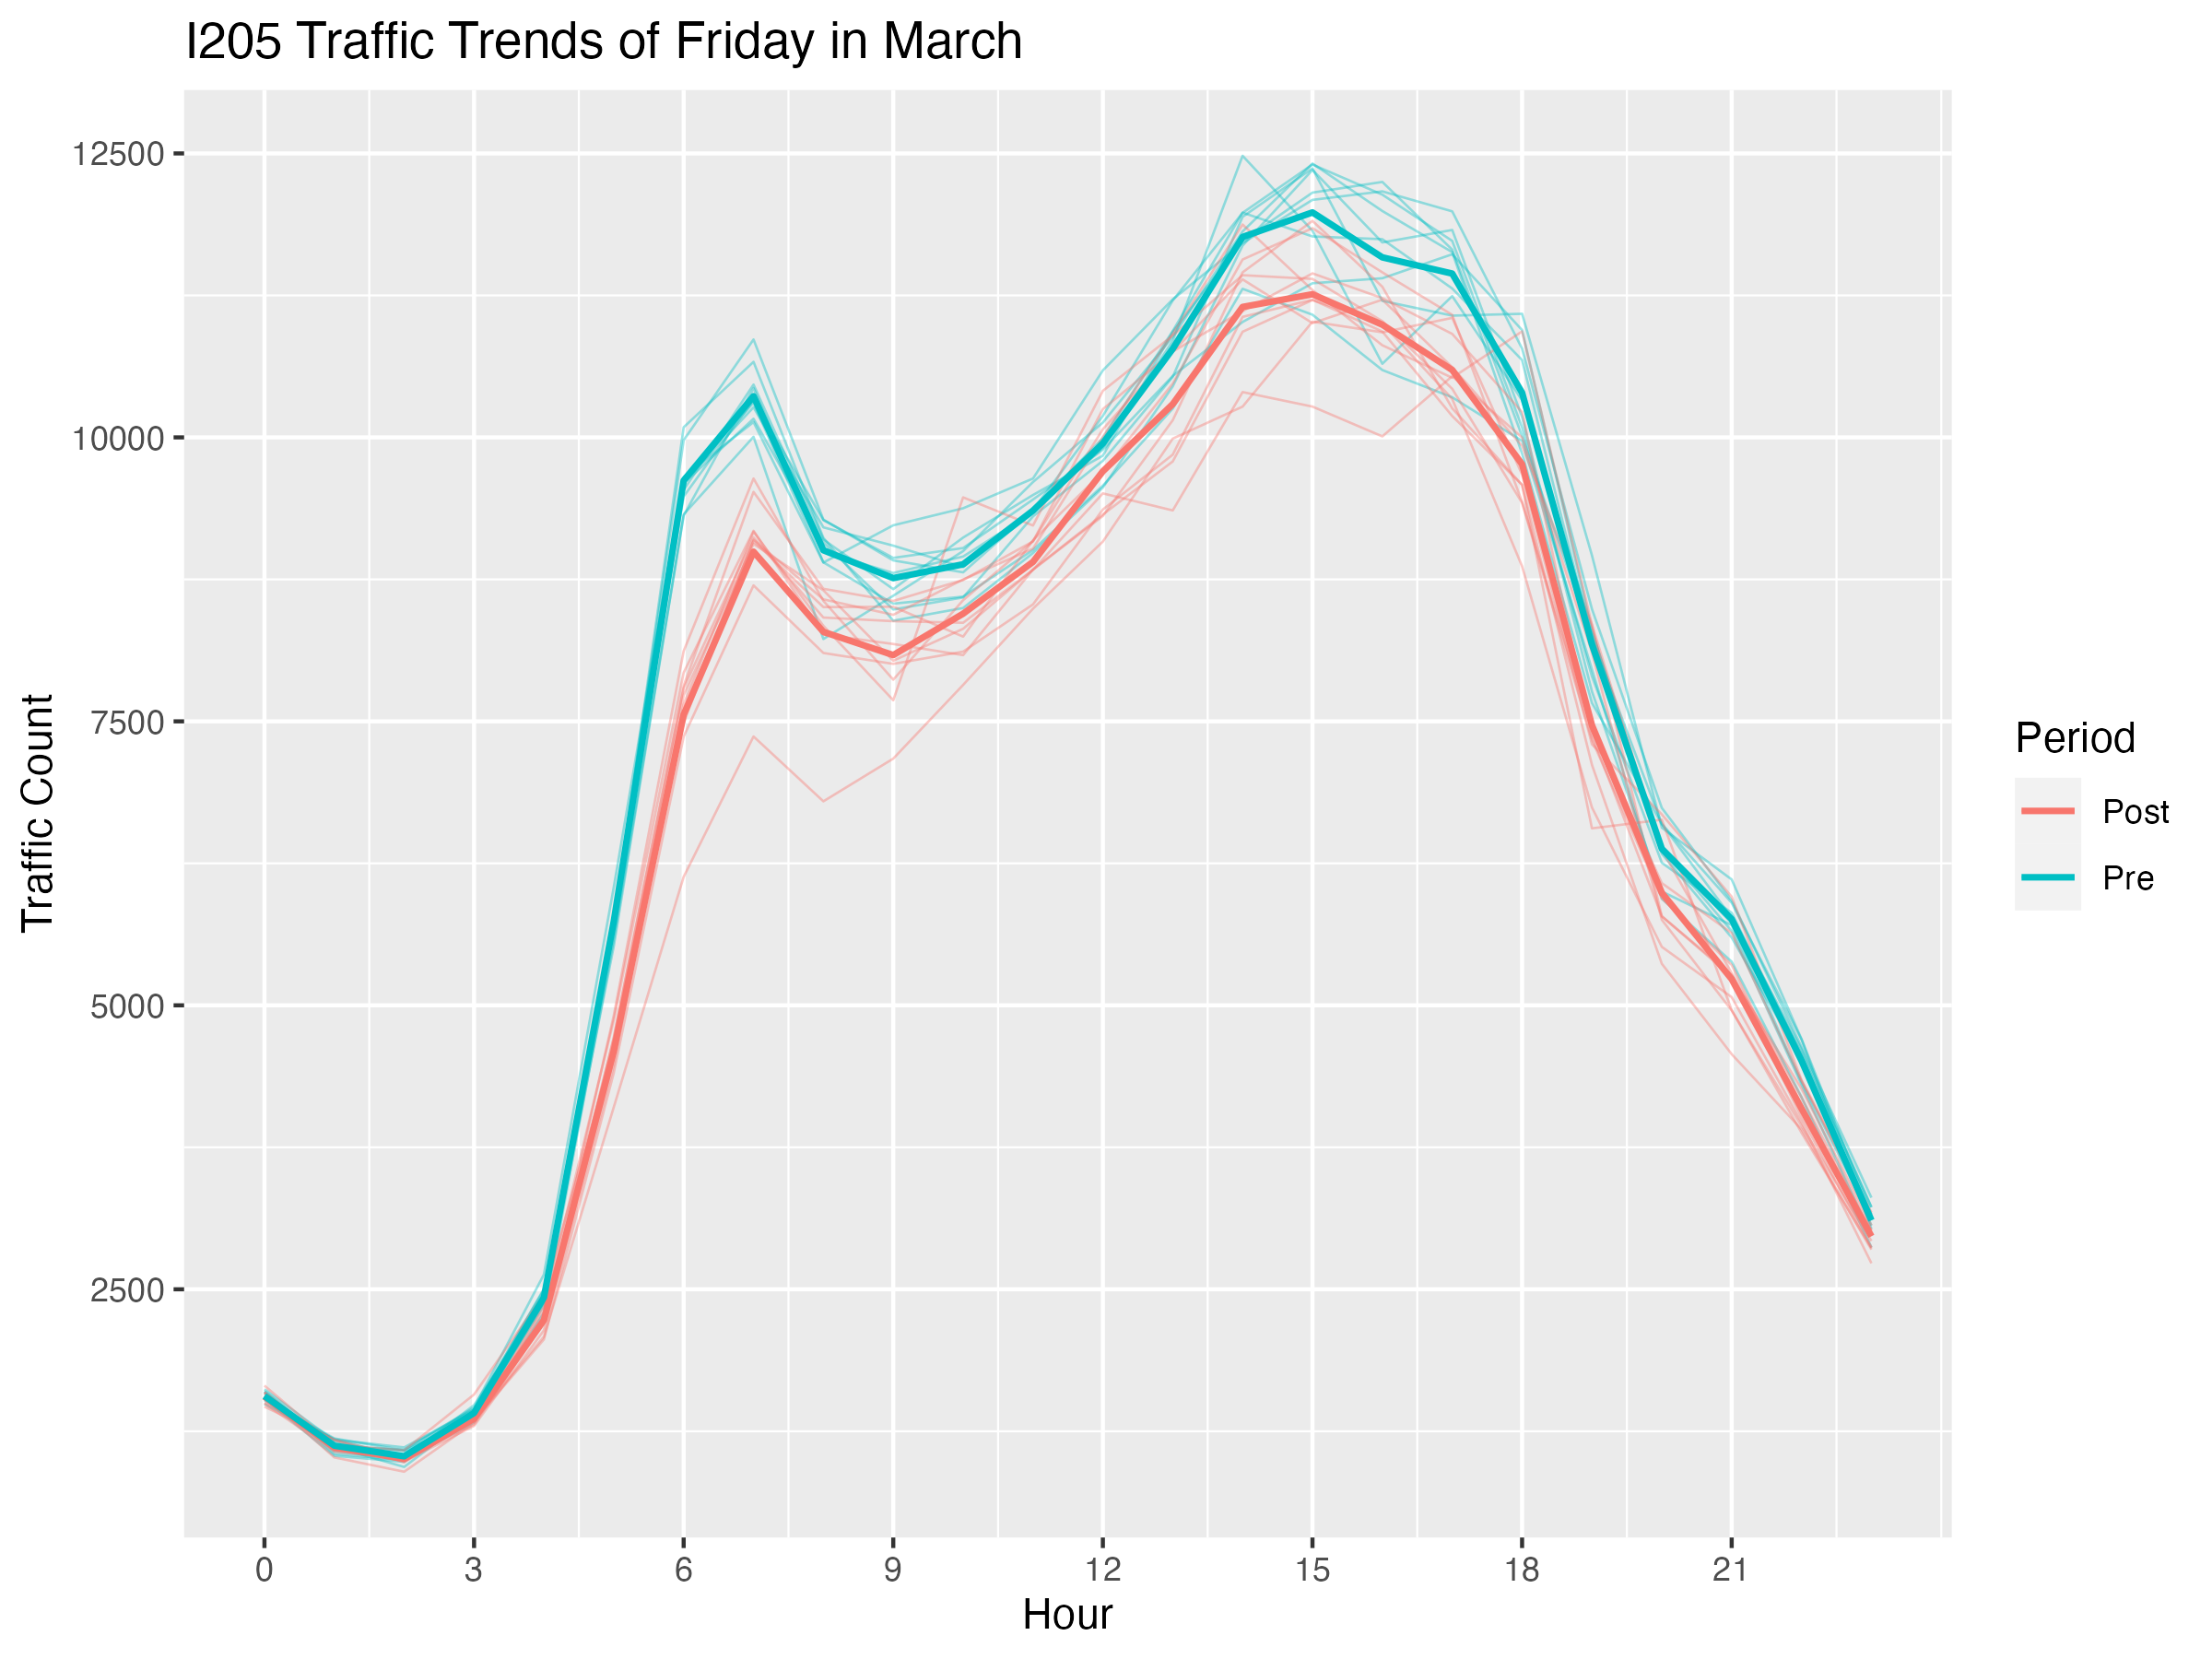
\includegraphics[width=\textwidth]{ATR26024_Plots/picture12_A24.png}
	\end{subfigure}
\end{figure}

\begin{figure}[H]
	\centering
	\begin{subfigure}[b]{0.45\textwidth}
		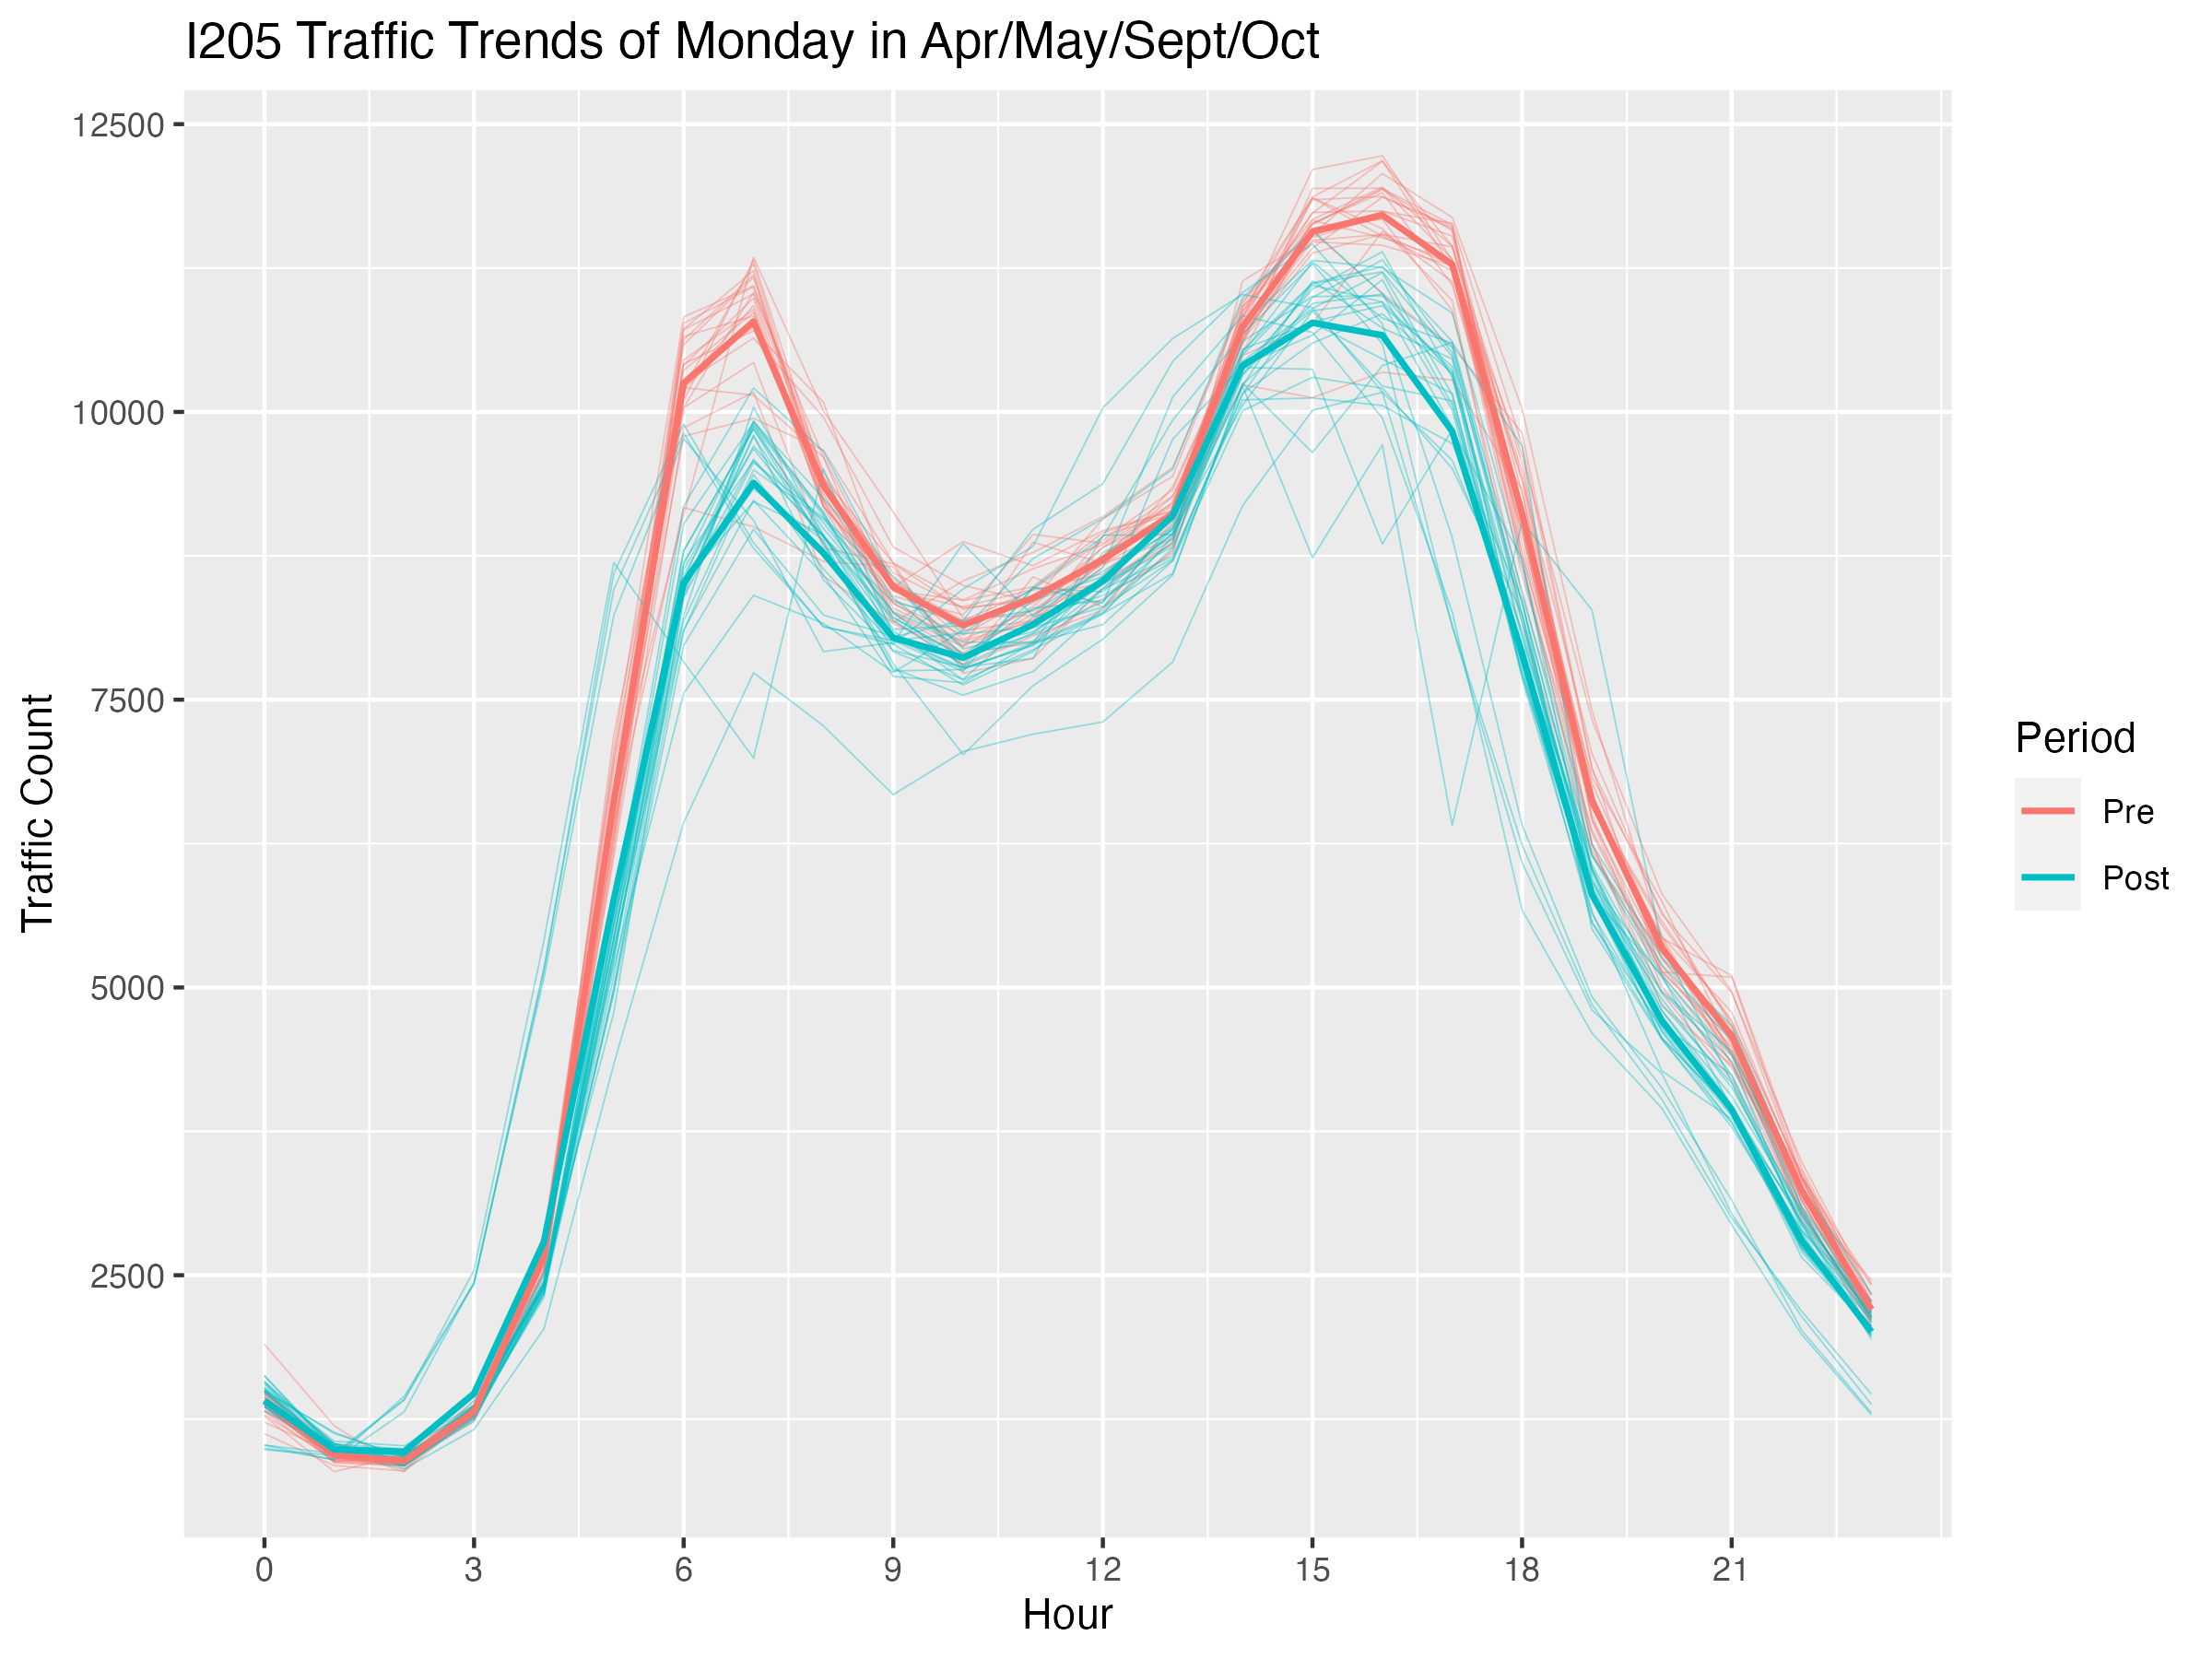
\includegraphics[width=\textwidth]{ATR26024_Plots/picture3_A24.png}
	\end{subfigure}
	\hfill
	\begin{subfigure}[b]{0.45\textwidth}
		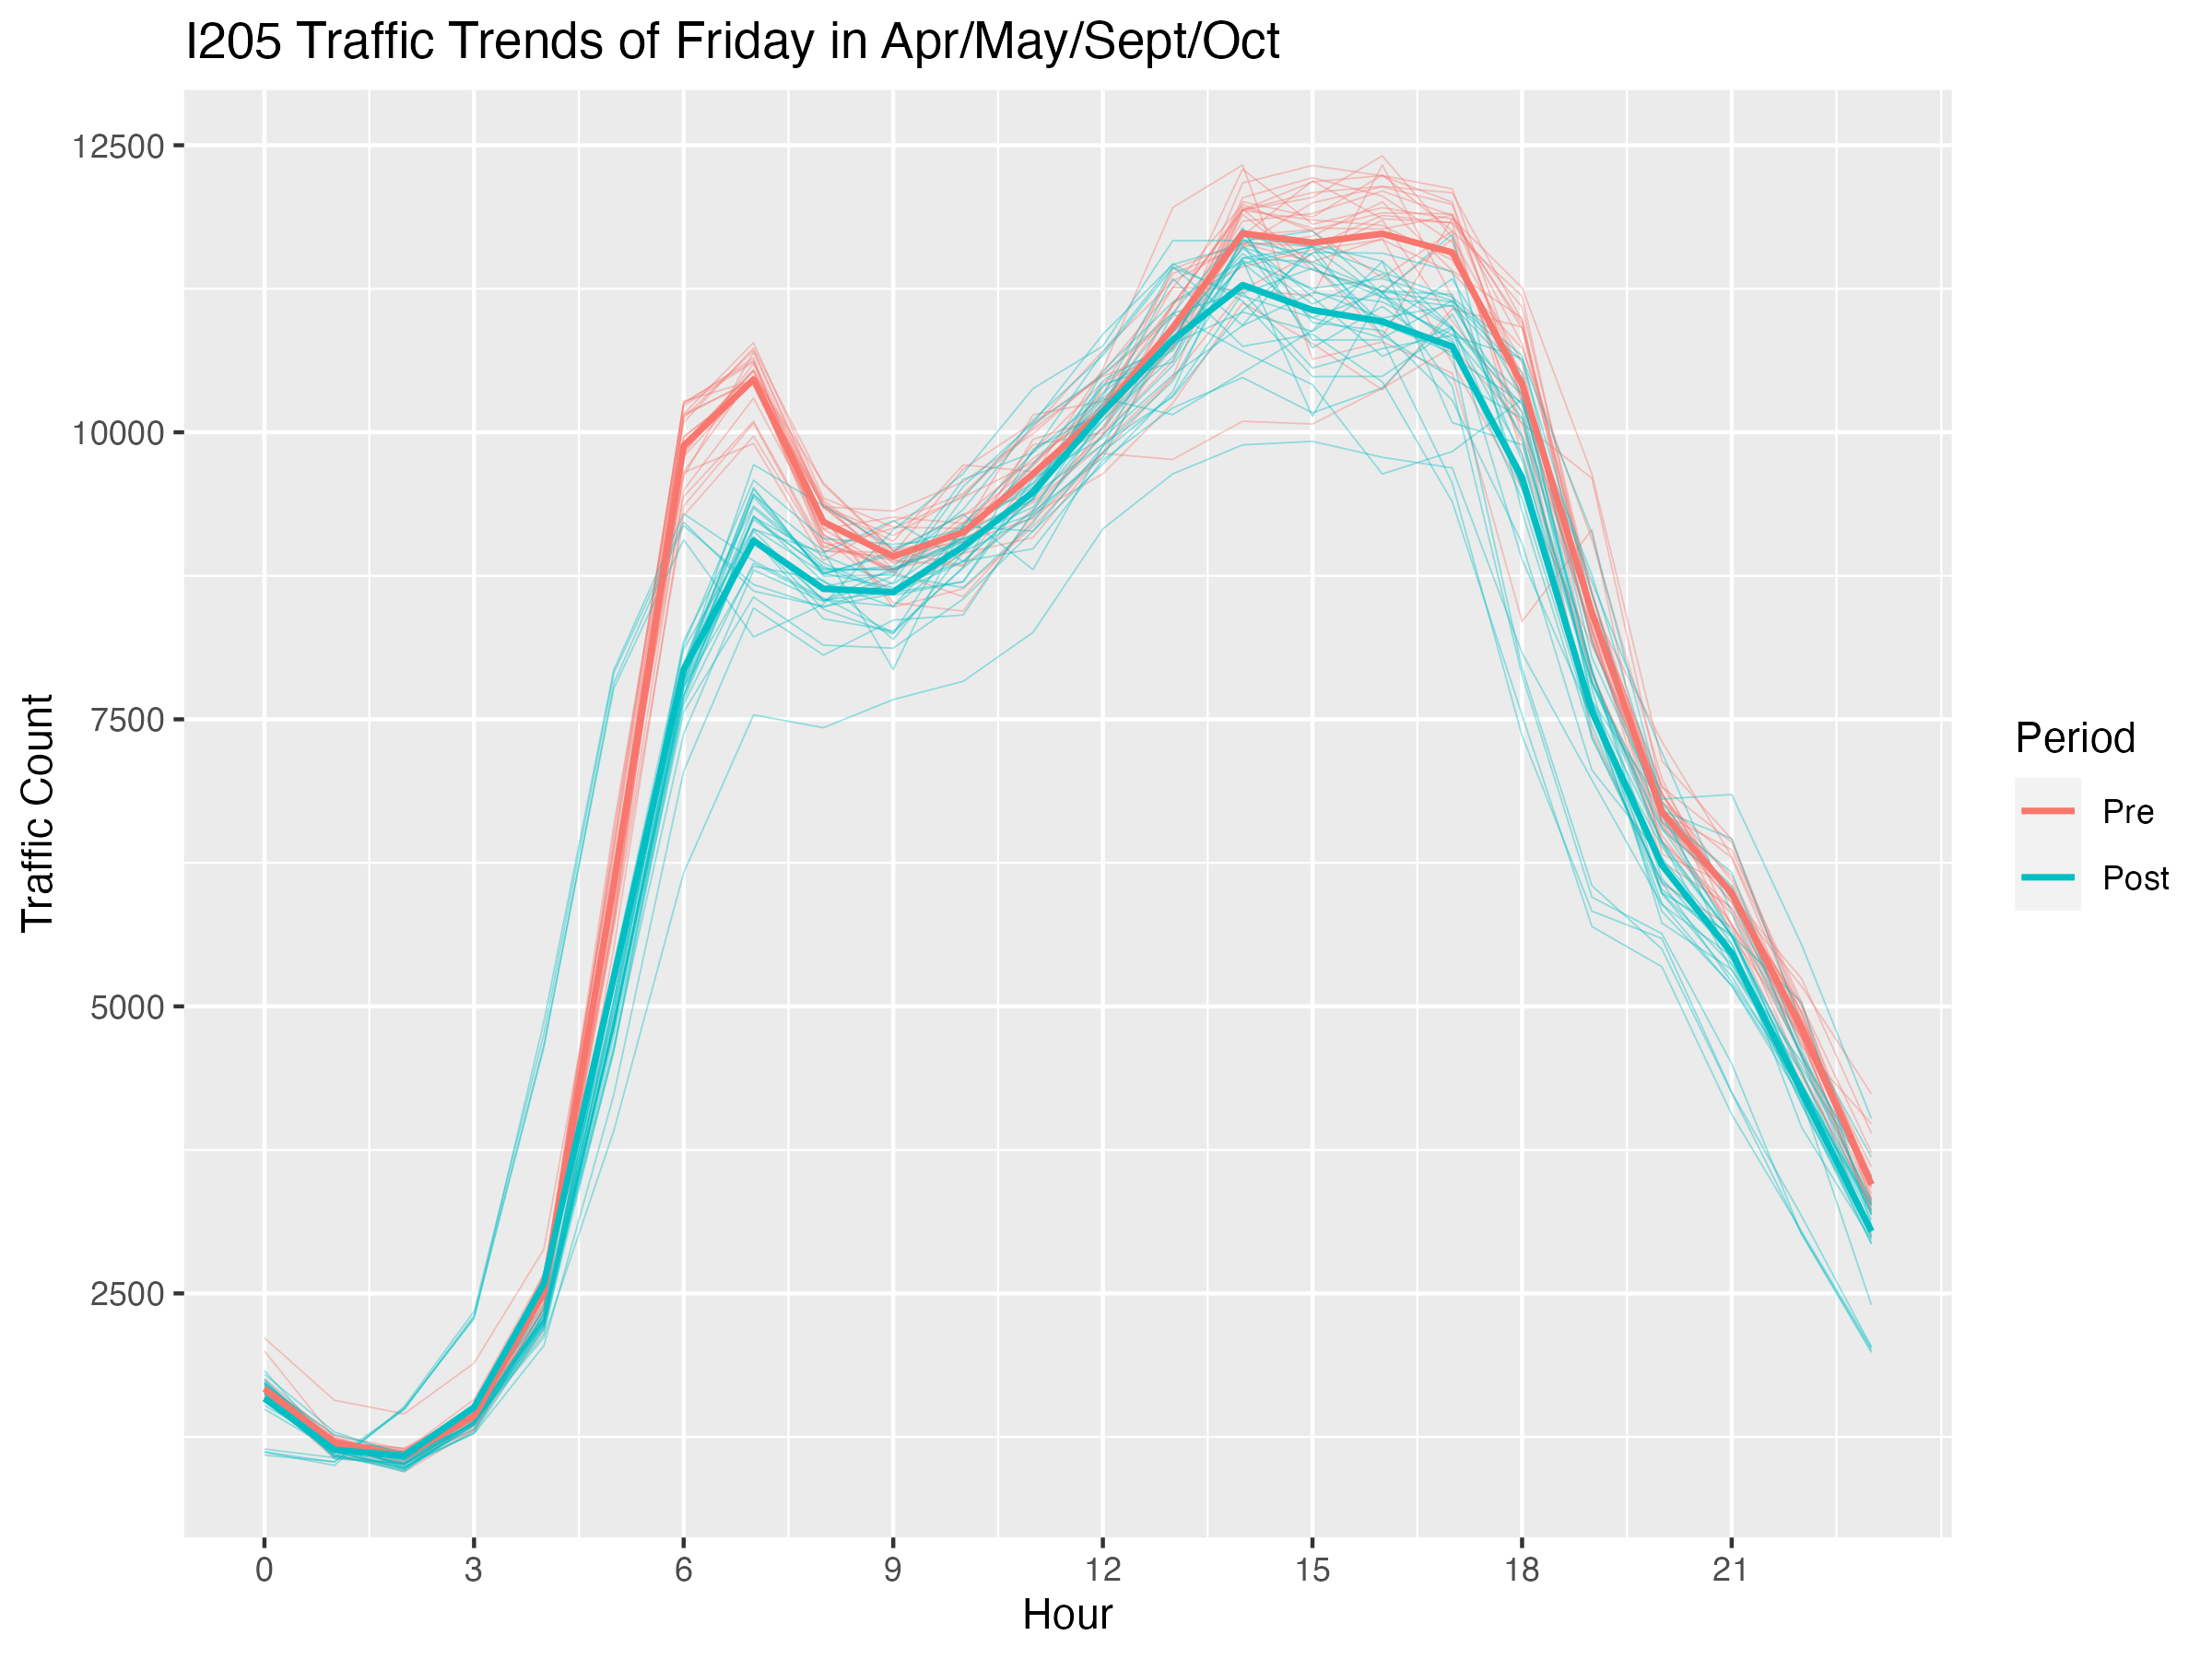
\includegraphics[width=\textwidth]{ATR26024_Plots/picture13_A24.png}
	\end{subfigure}
\end{figure}

\begin{figure}[H]
	\centering
	\begin{subfigure}[b]{0.45\textwidth}
		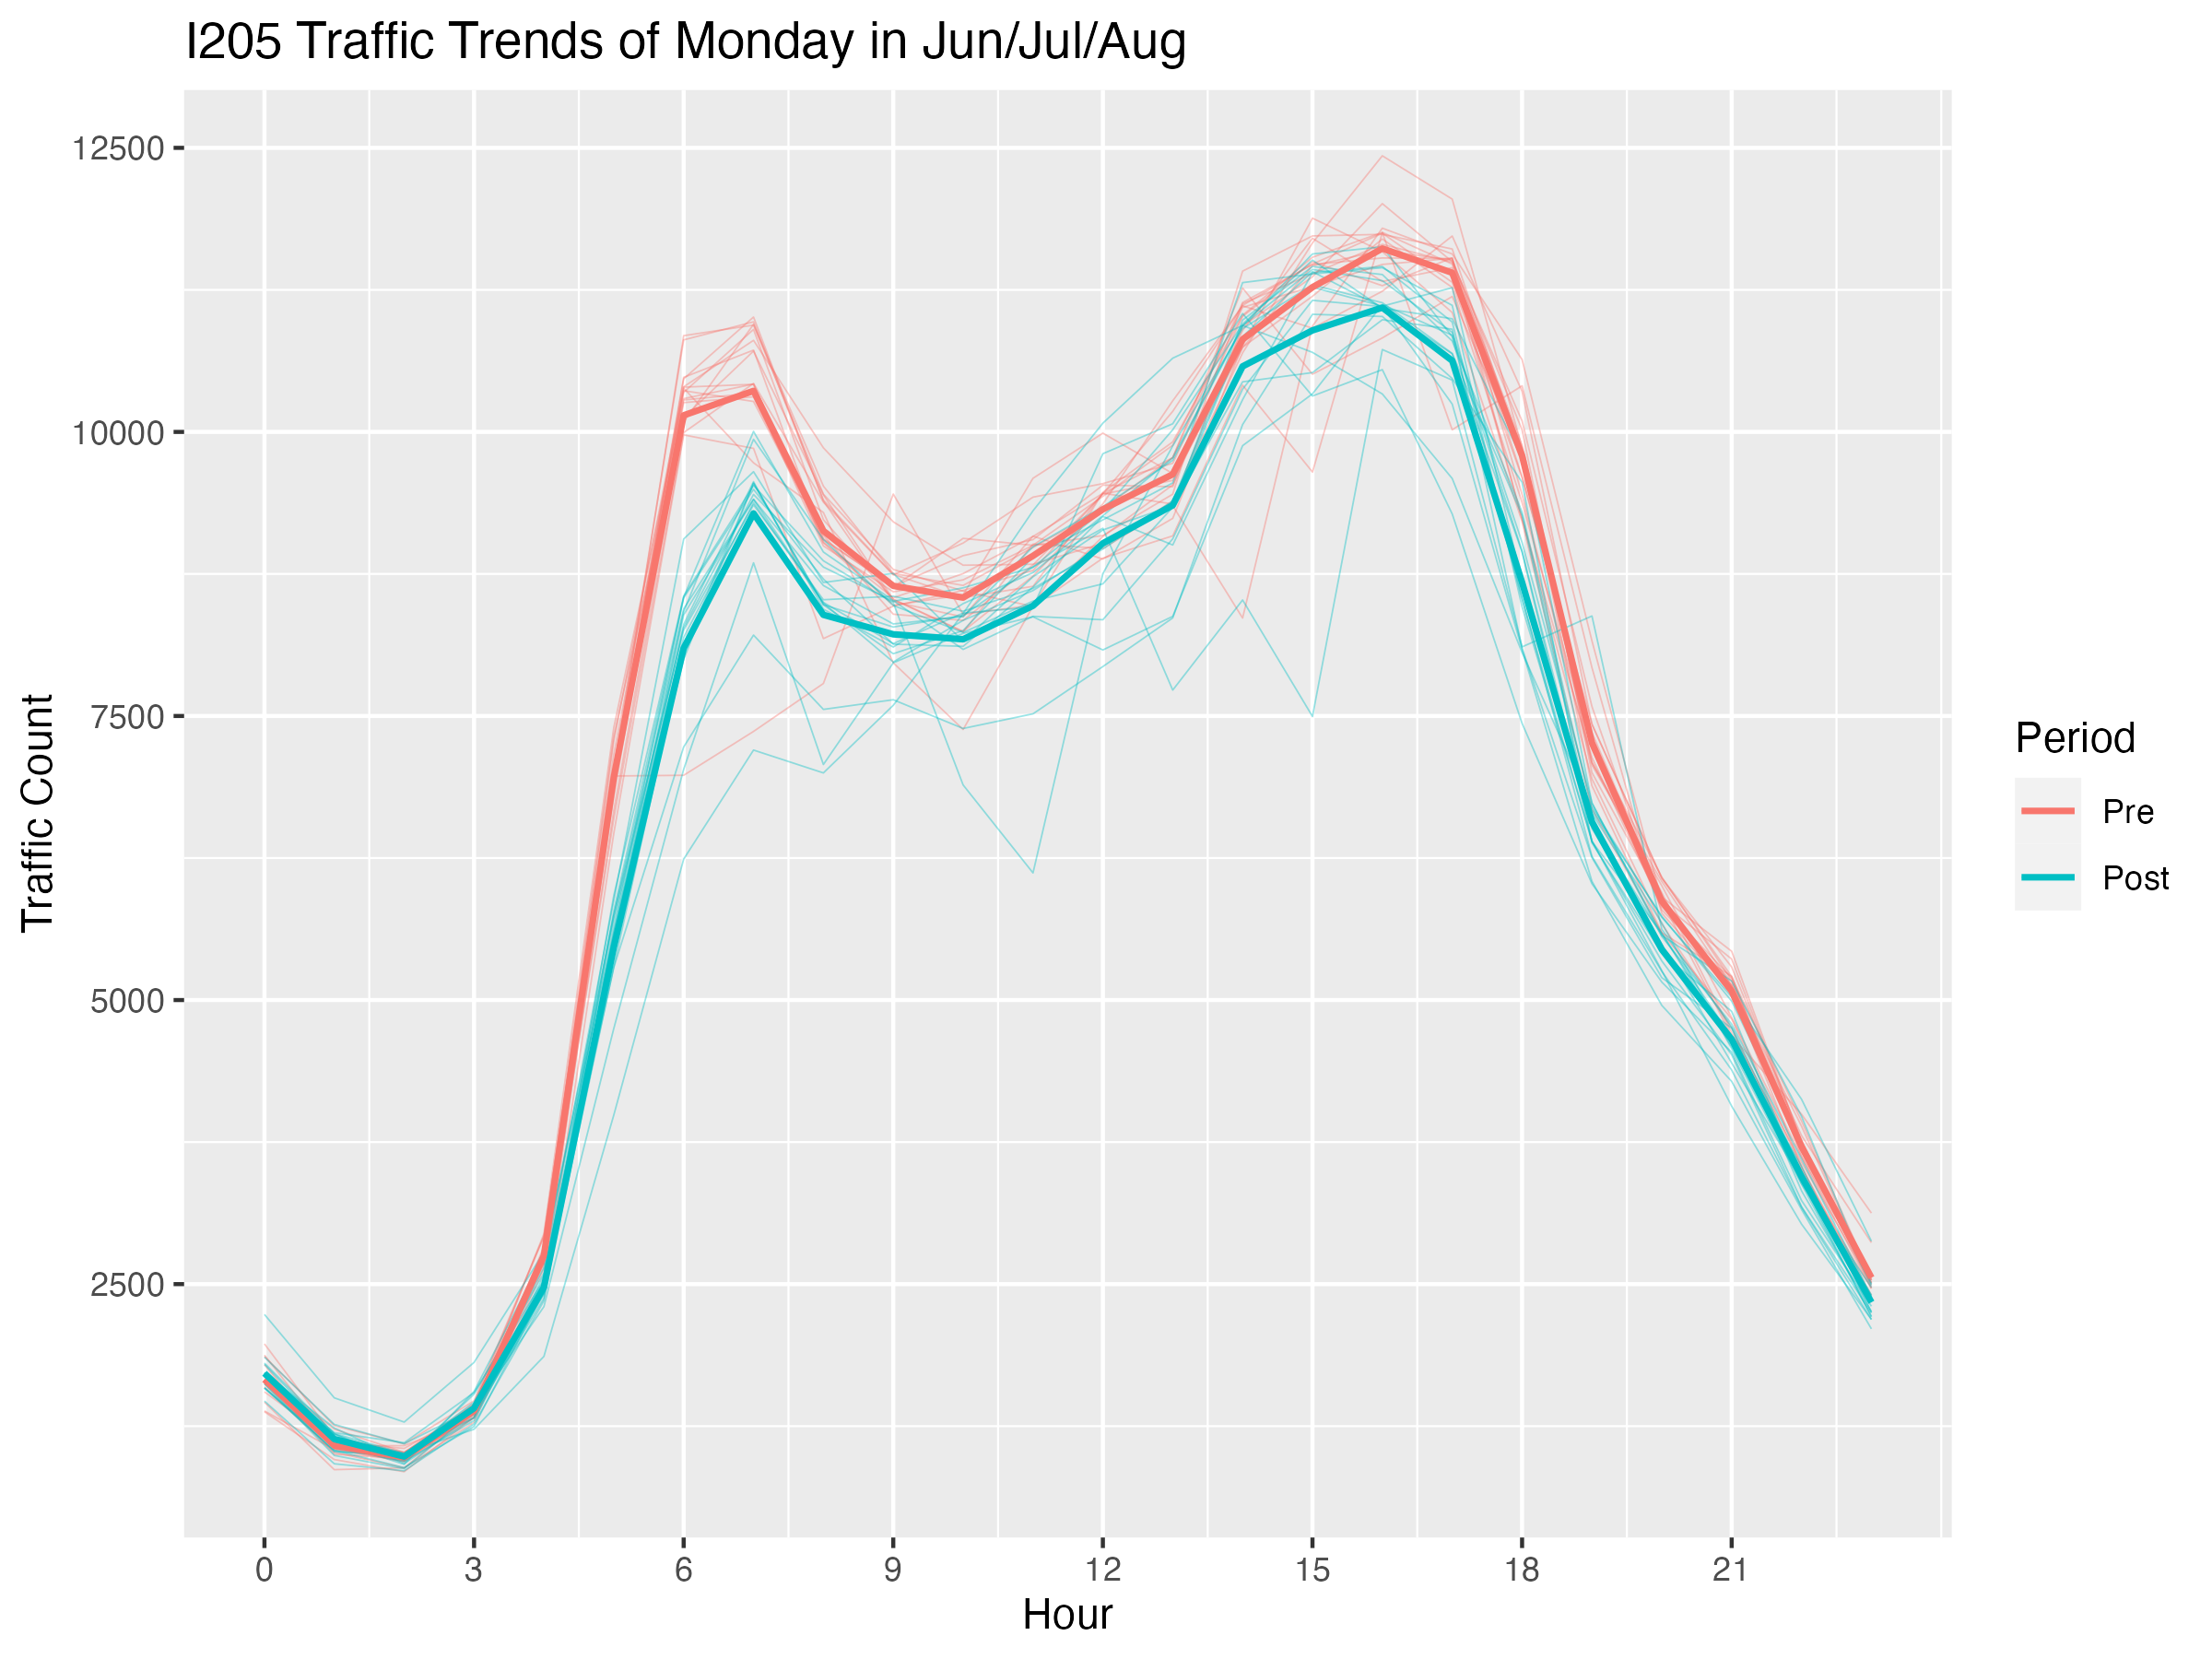
\includegraphics[width=\textwidth]{ATR26024_Plots/picture4_A24.png}
	\end{subfigure}
	\hfill
	\begin{subfigure}[b]{0.45\textwidth}
		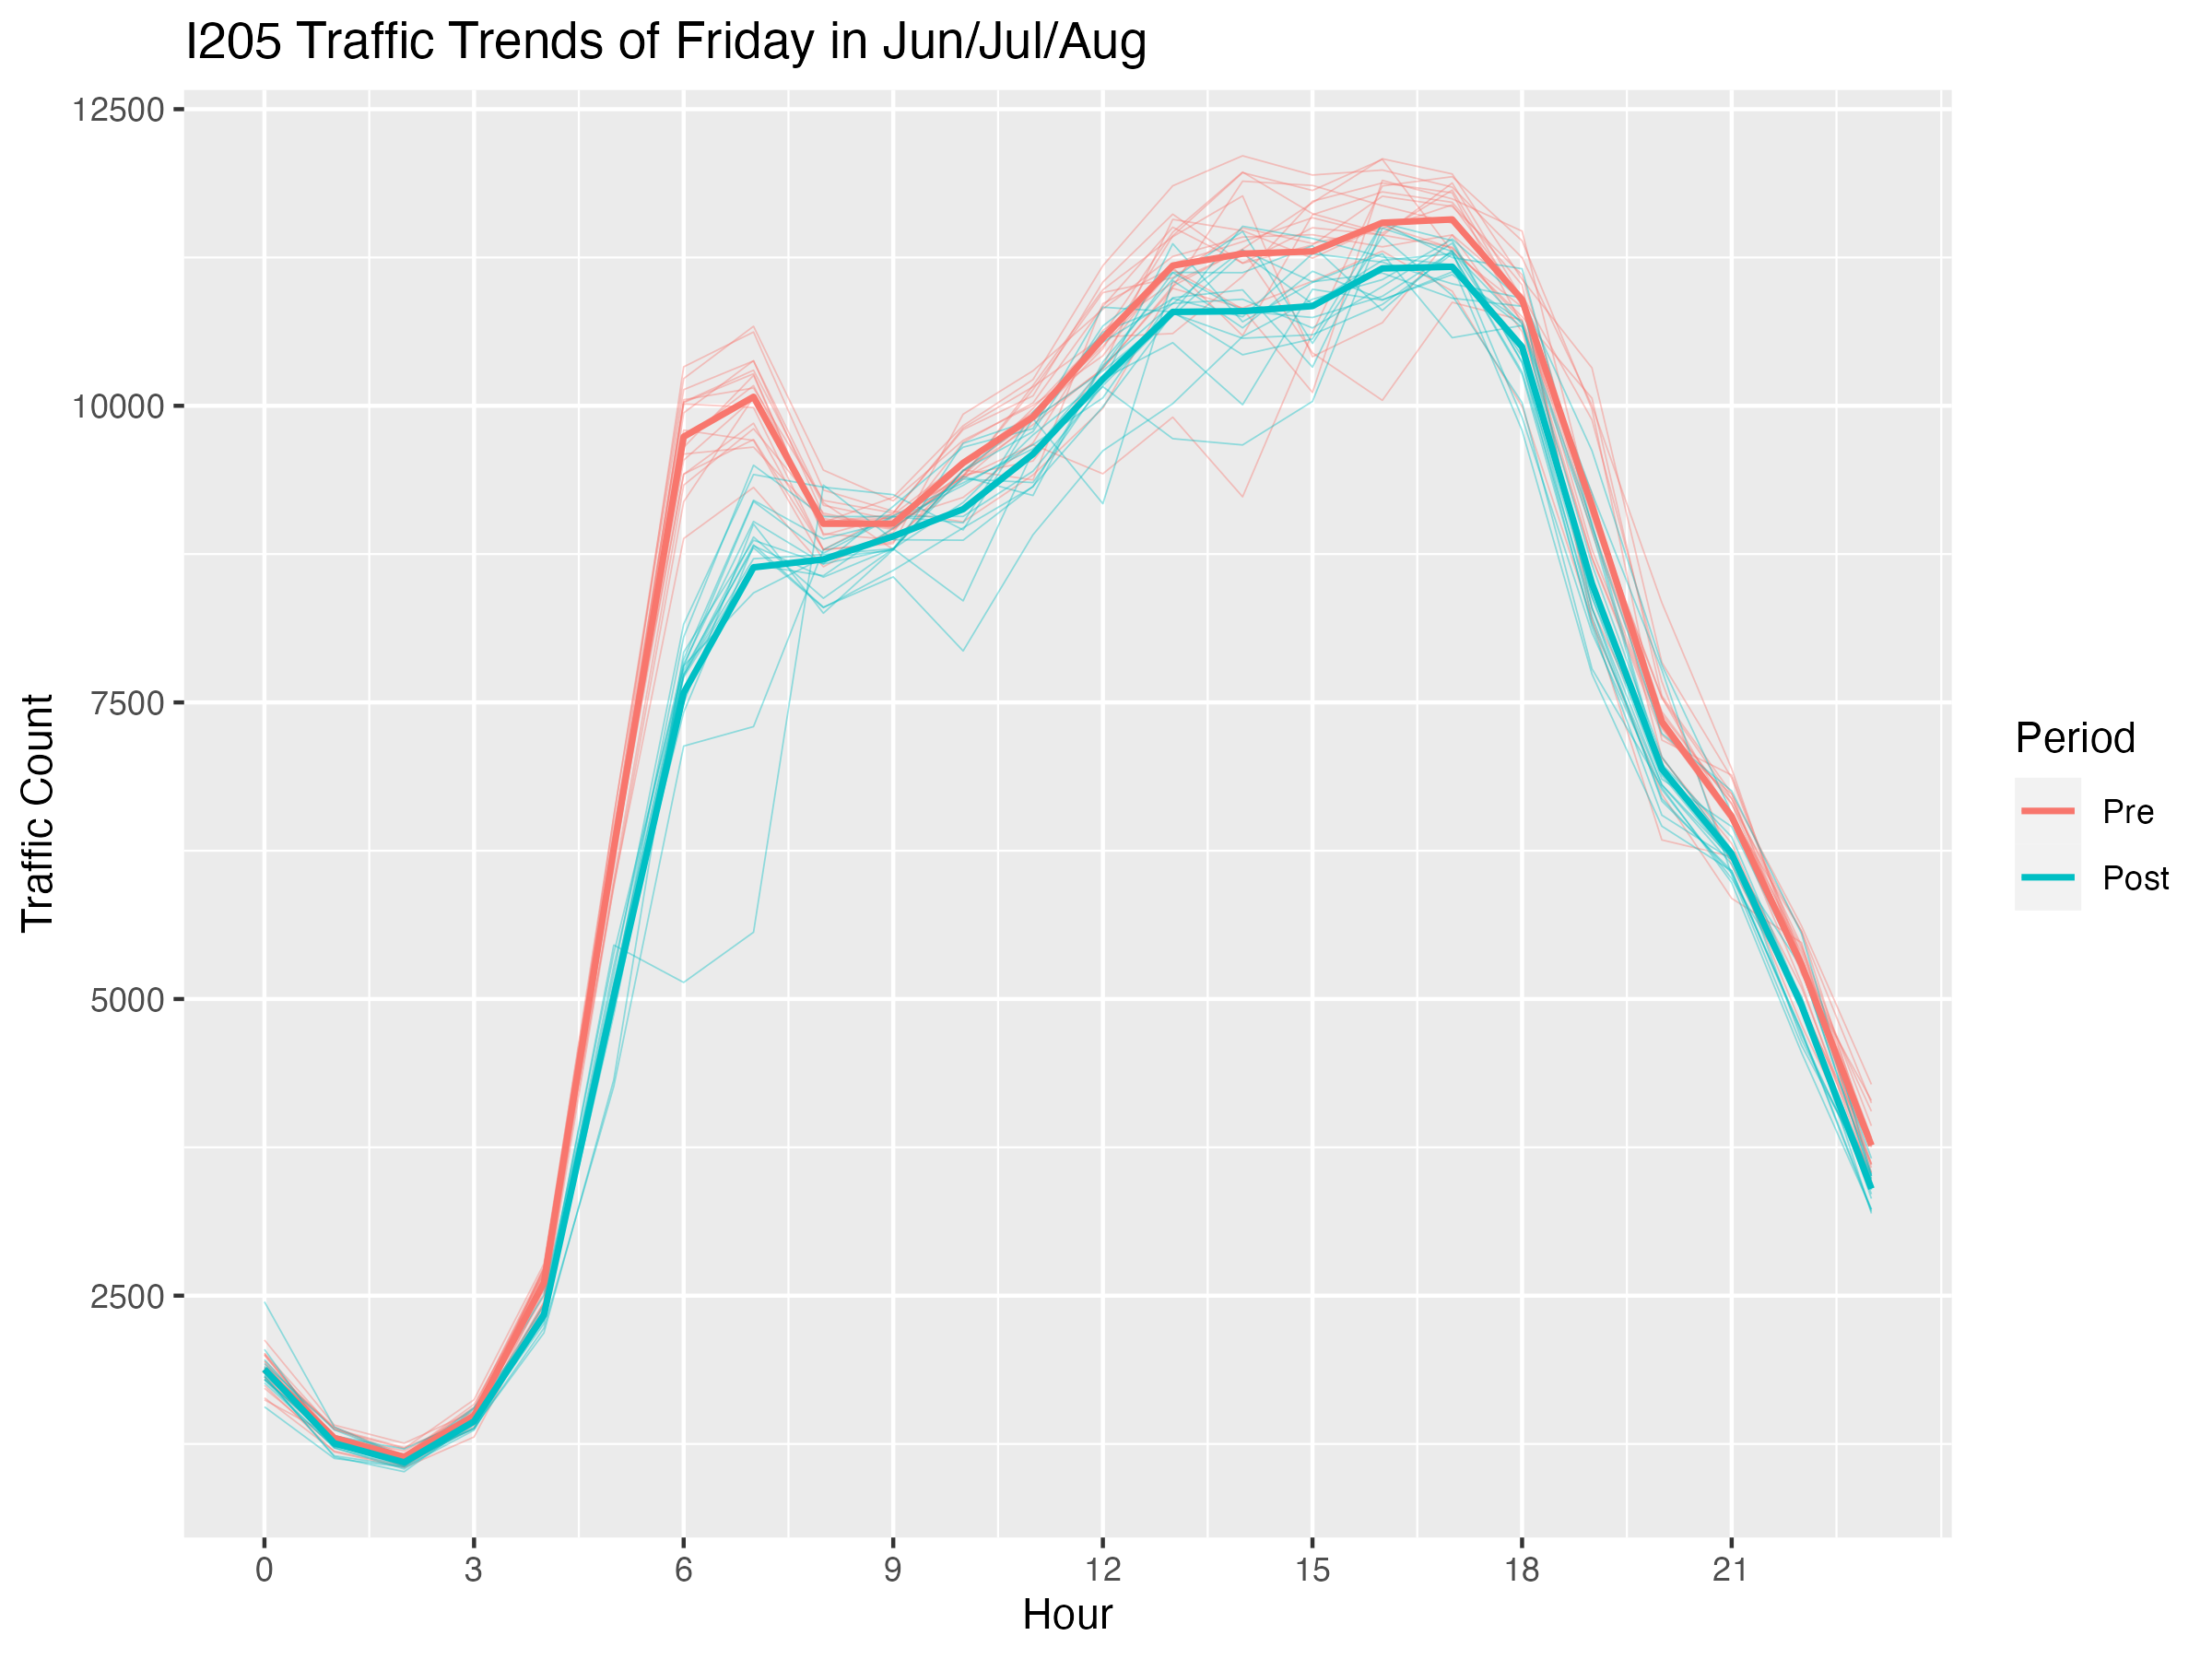
\includegraphics[width=\textwidth]{ATR26024_Plots/picture14_A24.png}
	\end{subfigure}
\end{figure}

\begin{figure}[H]
	\centering
	\begin{subfigure}[b]{0.45\textwidth}
		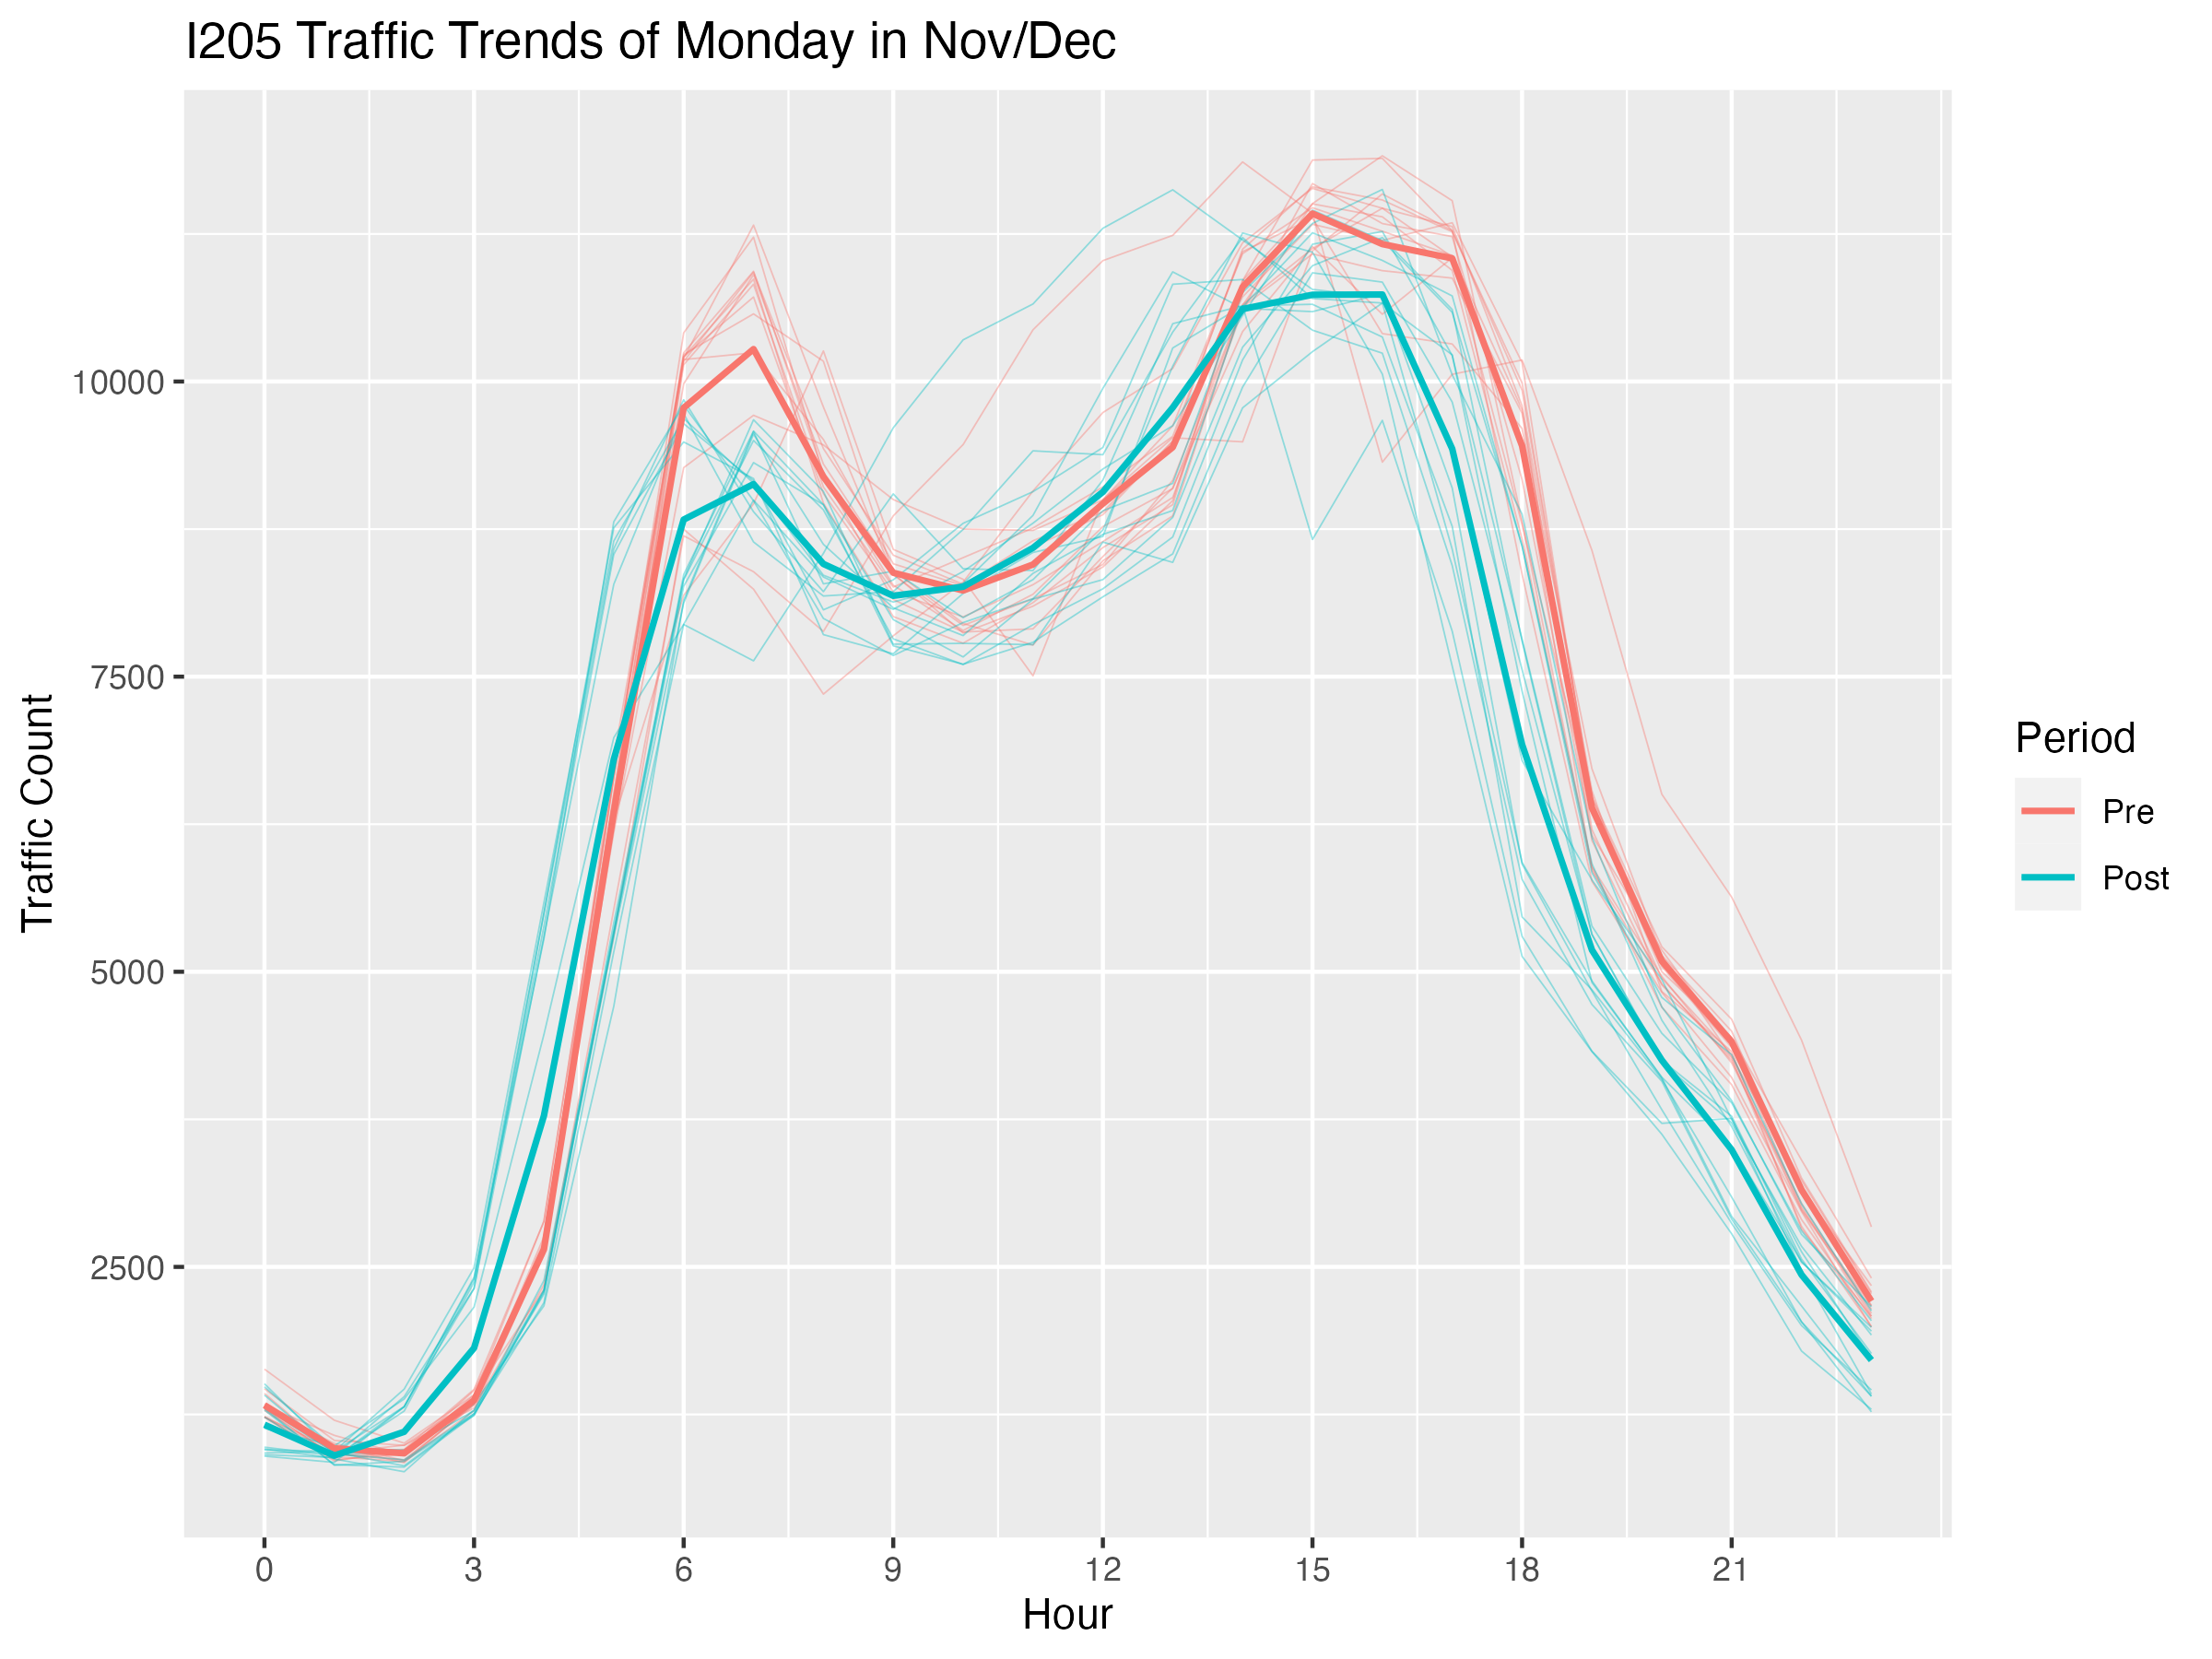
\includegraphics[width=\textwidth]{ATR26024_Plots/picture5_A24.png}
	\end{subfigure}
	\hfill
	\begin{subfigure}[b]{0.45\textwidth}
		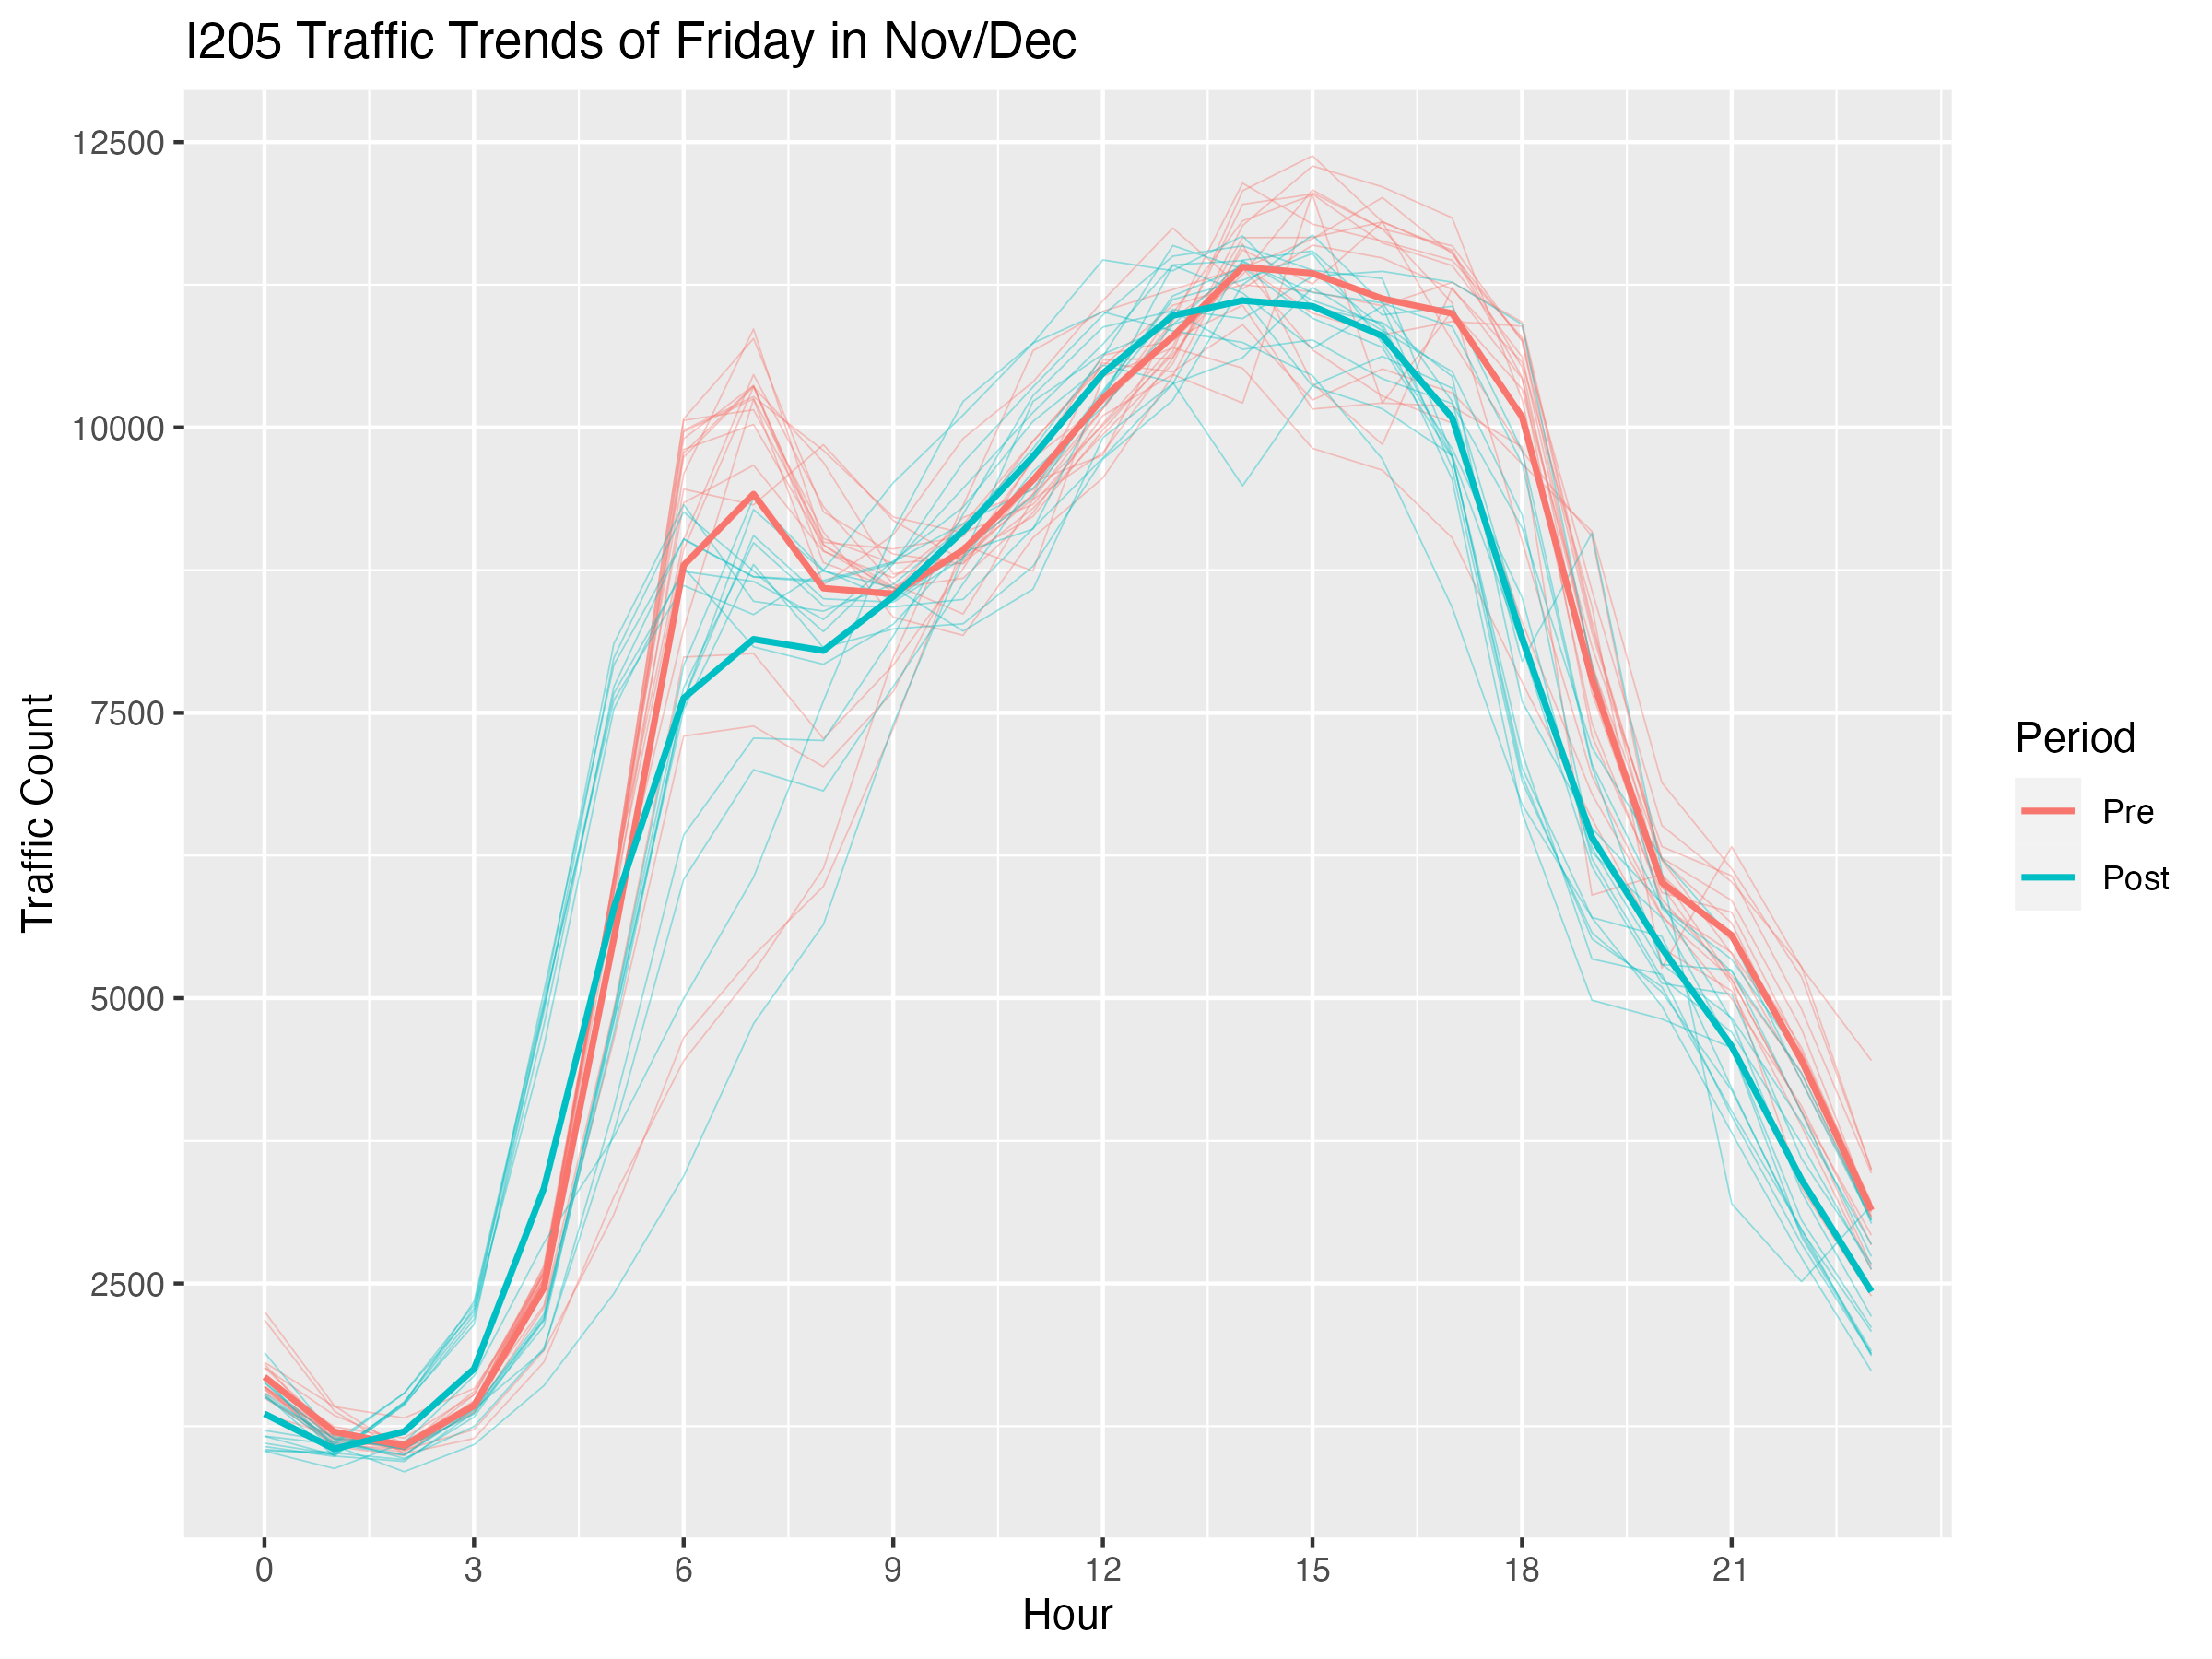
\includegraphics[width=\textwidth]{ATR26024_Plots/picture15_A24.png}
	\end{subfigure}
\end{figure}

\begin{figure}[H]
	\centering
	\begin{subfigure}[b]{0.45\textwidth}
		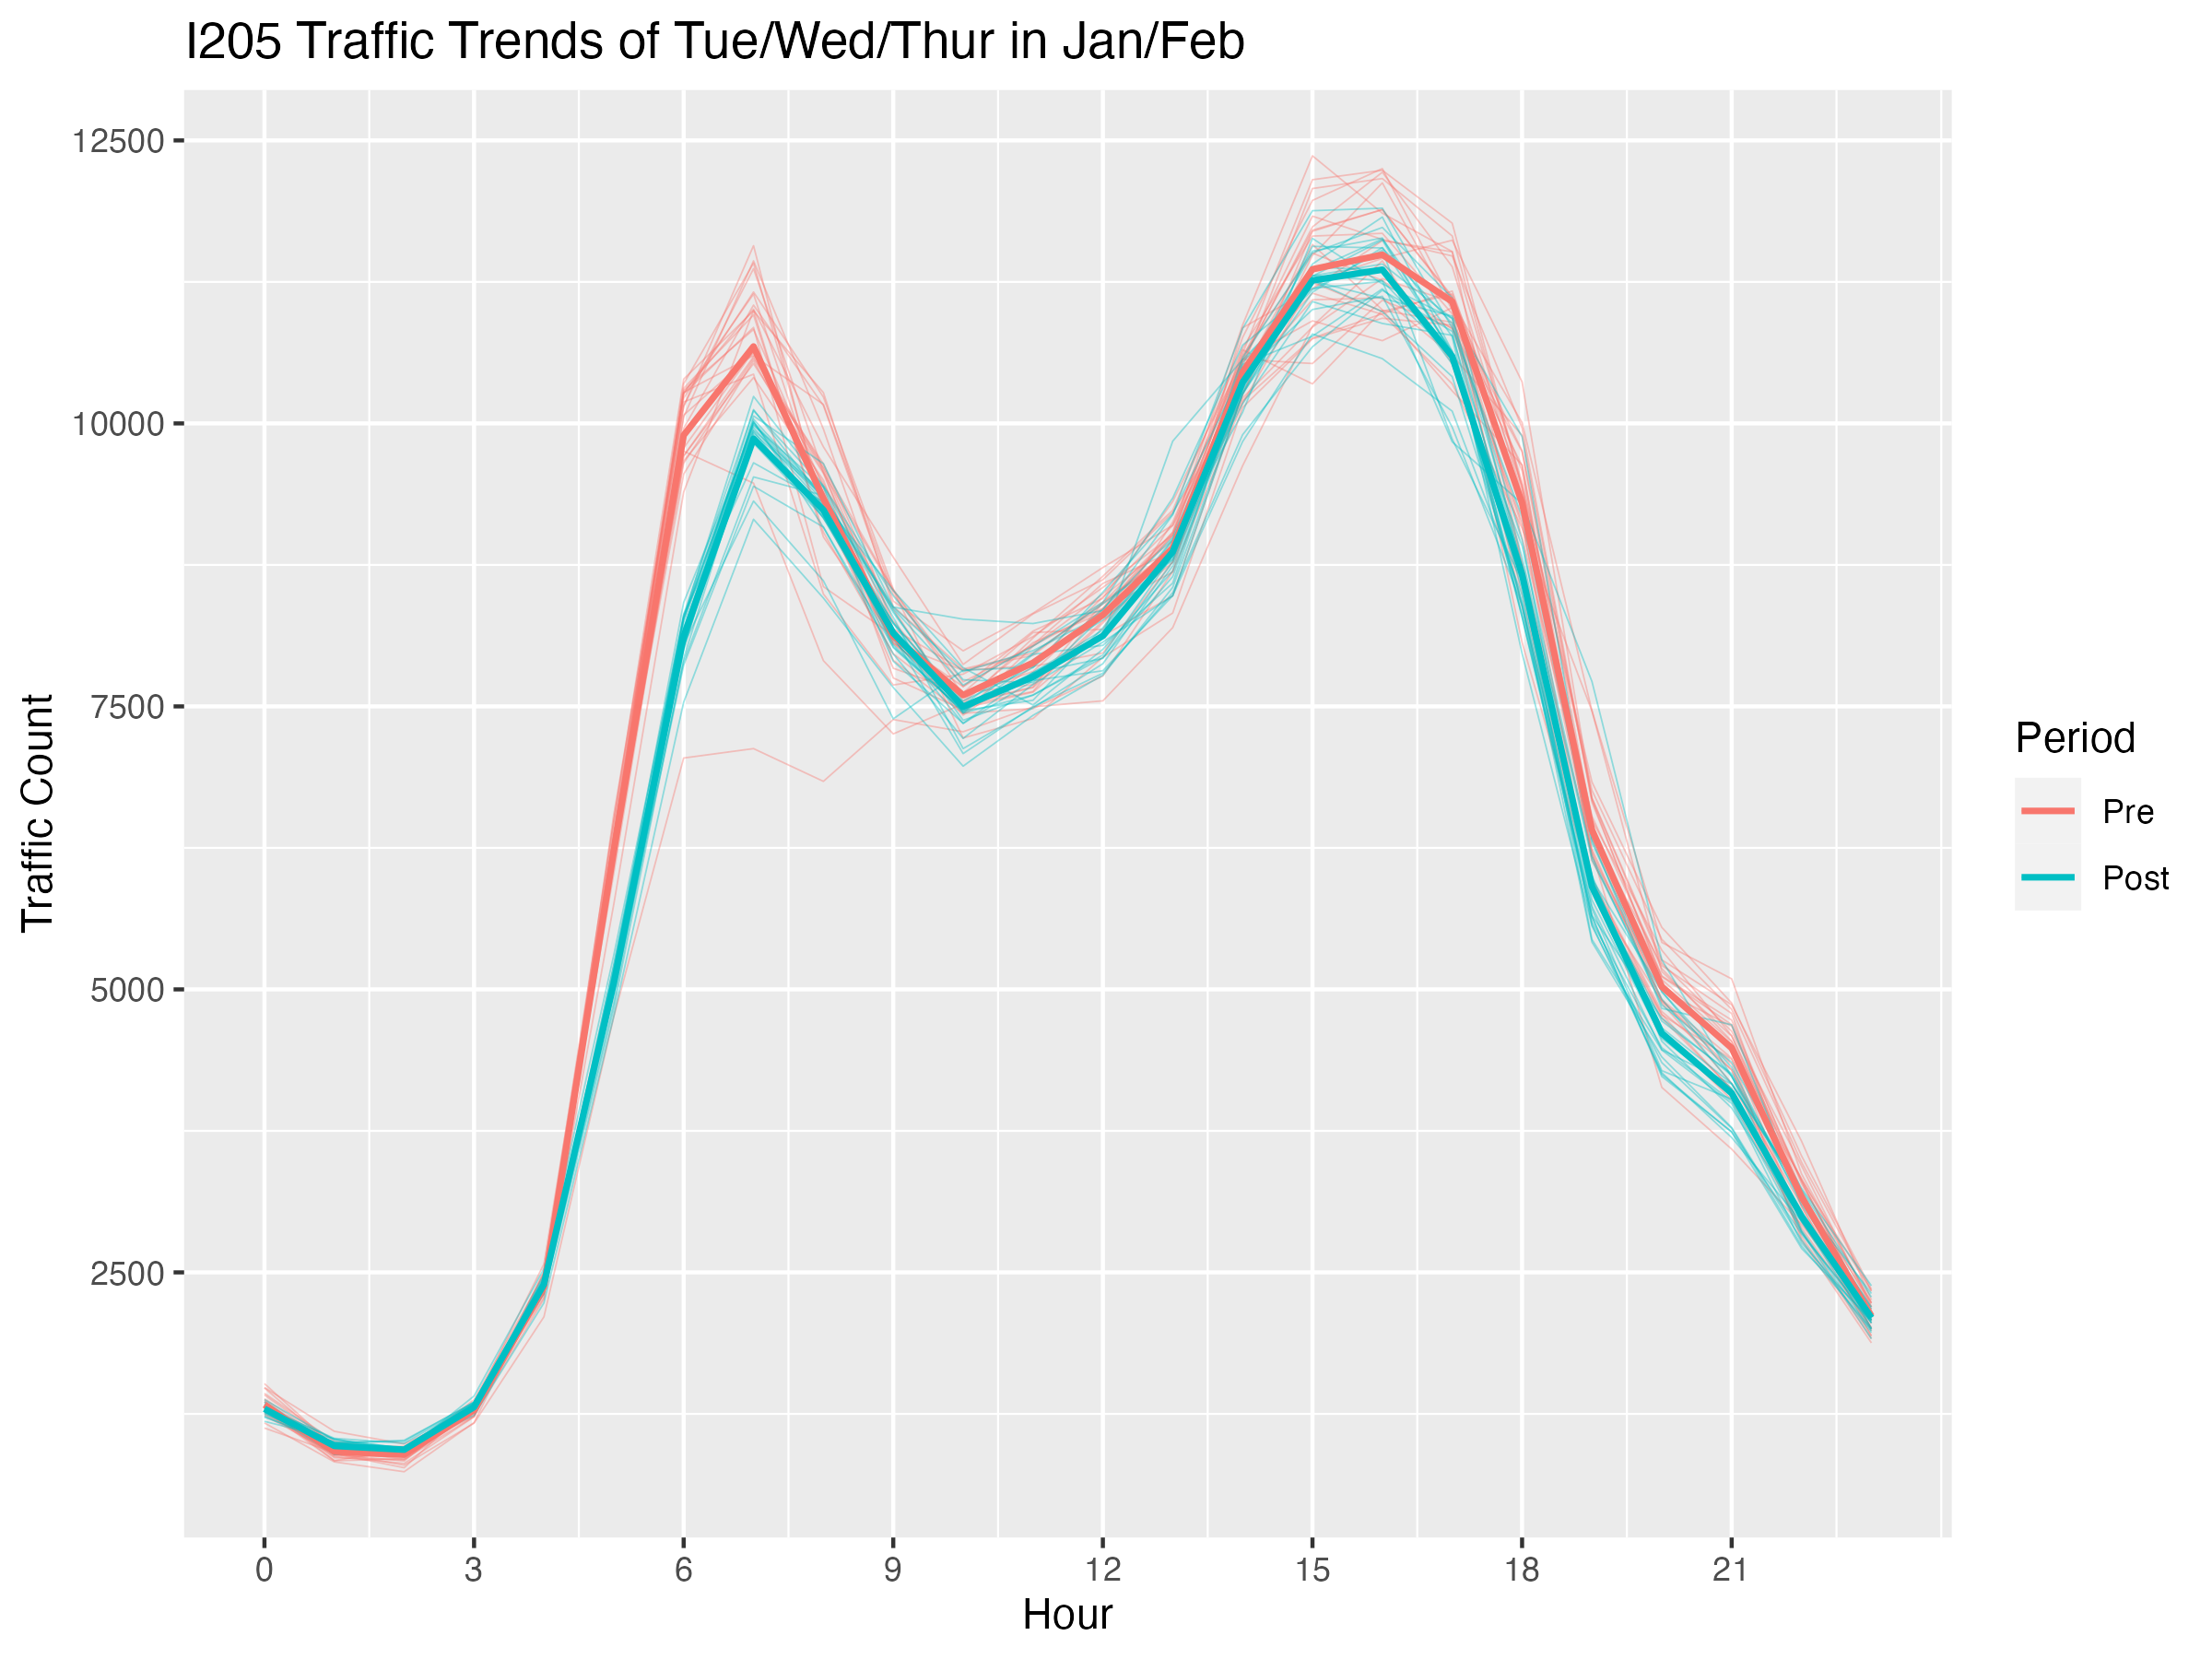
\includegraphics[width=\textwidth]{ATR26024_Plots/picture6_A24.png}
	\end{subfigure}
	\hfill
	\begin{subfigure}[b]{0.45\textwidth}
		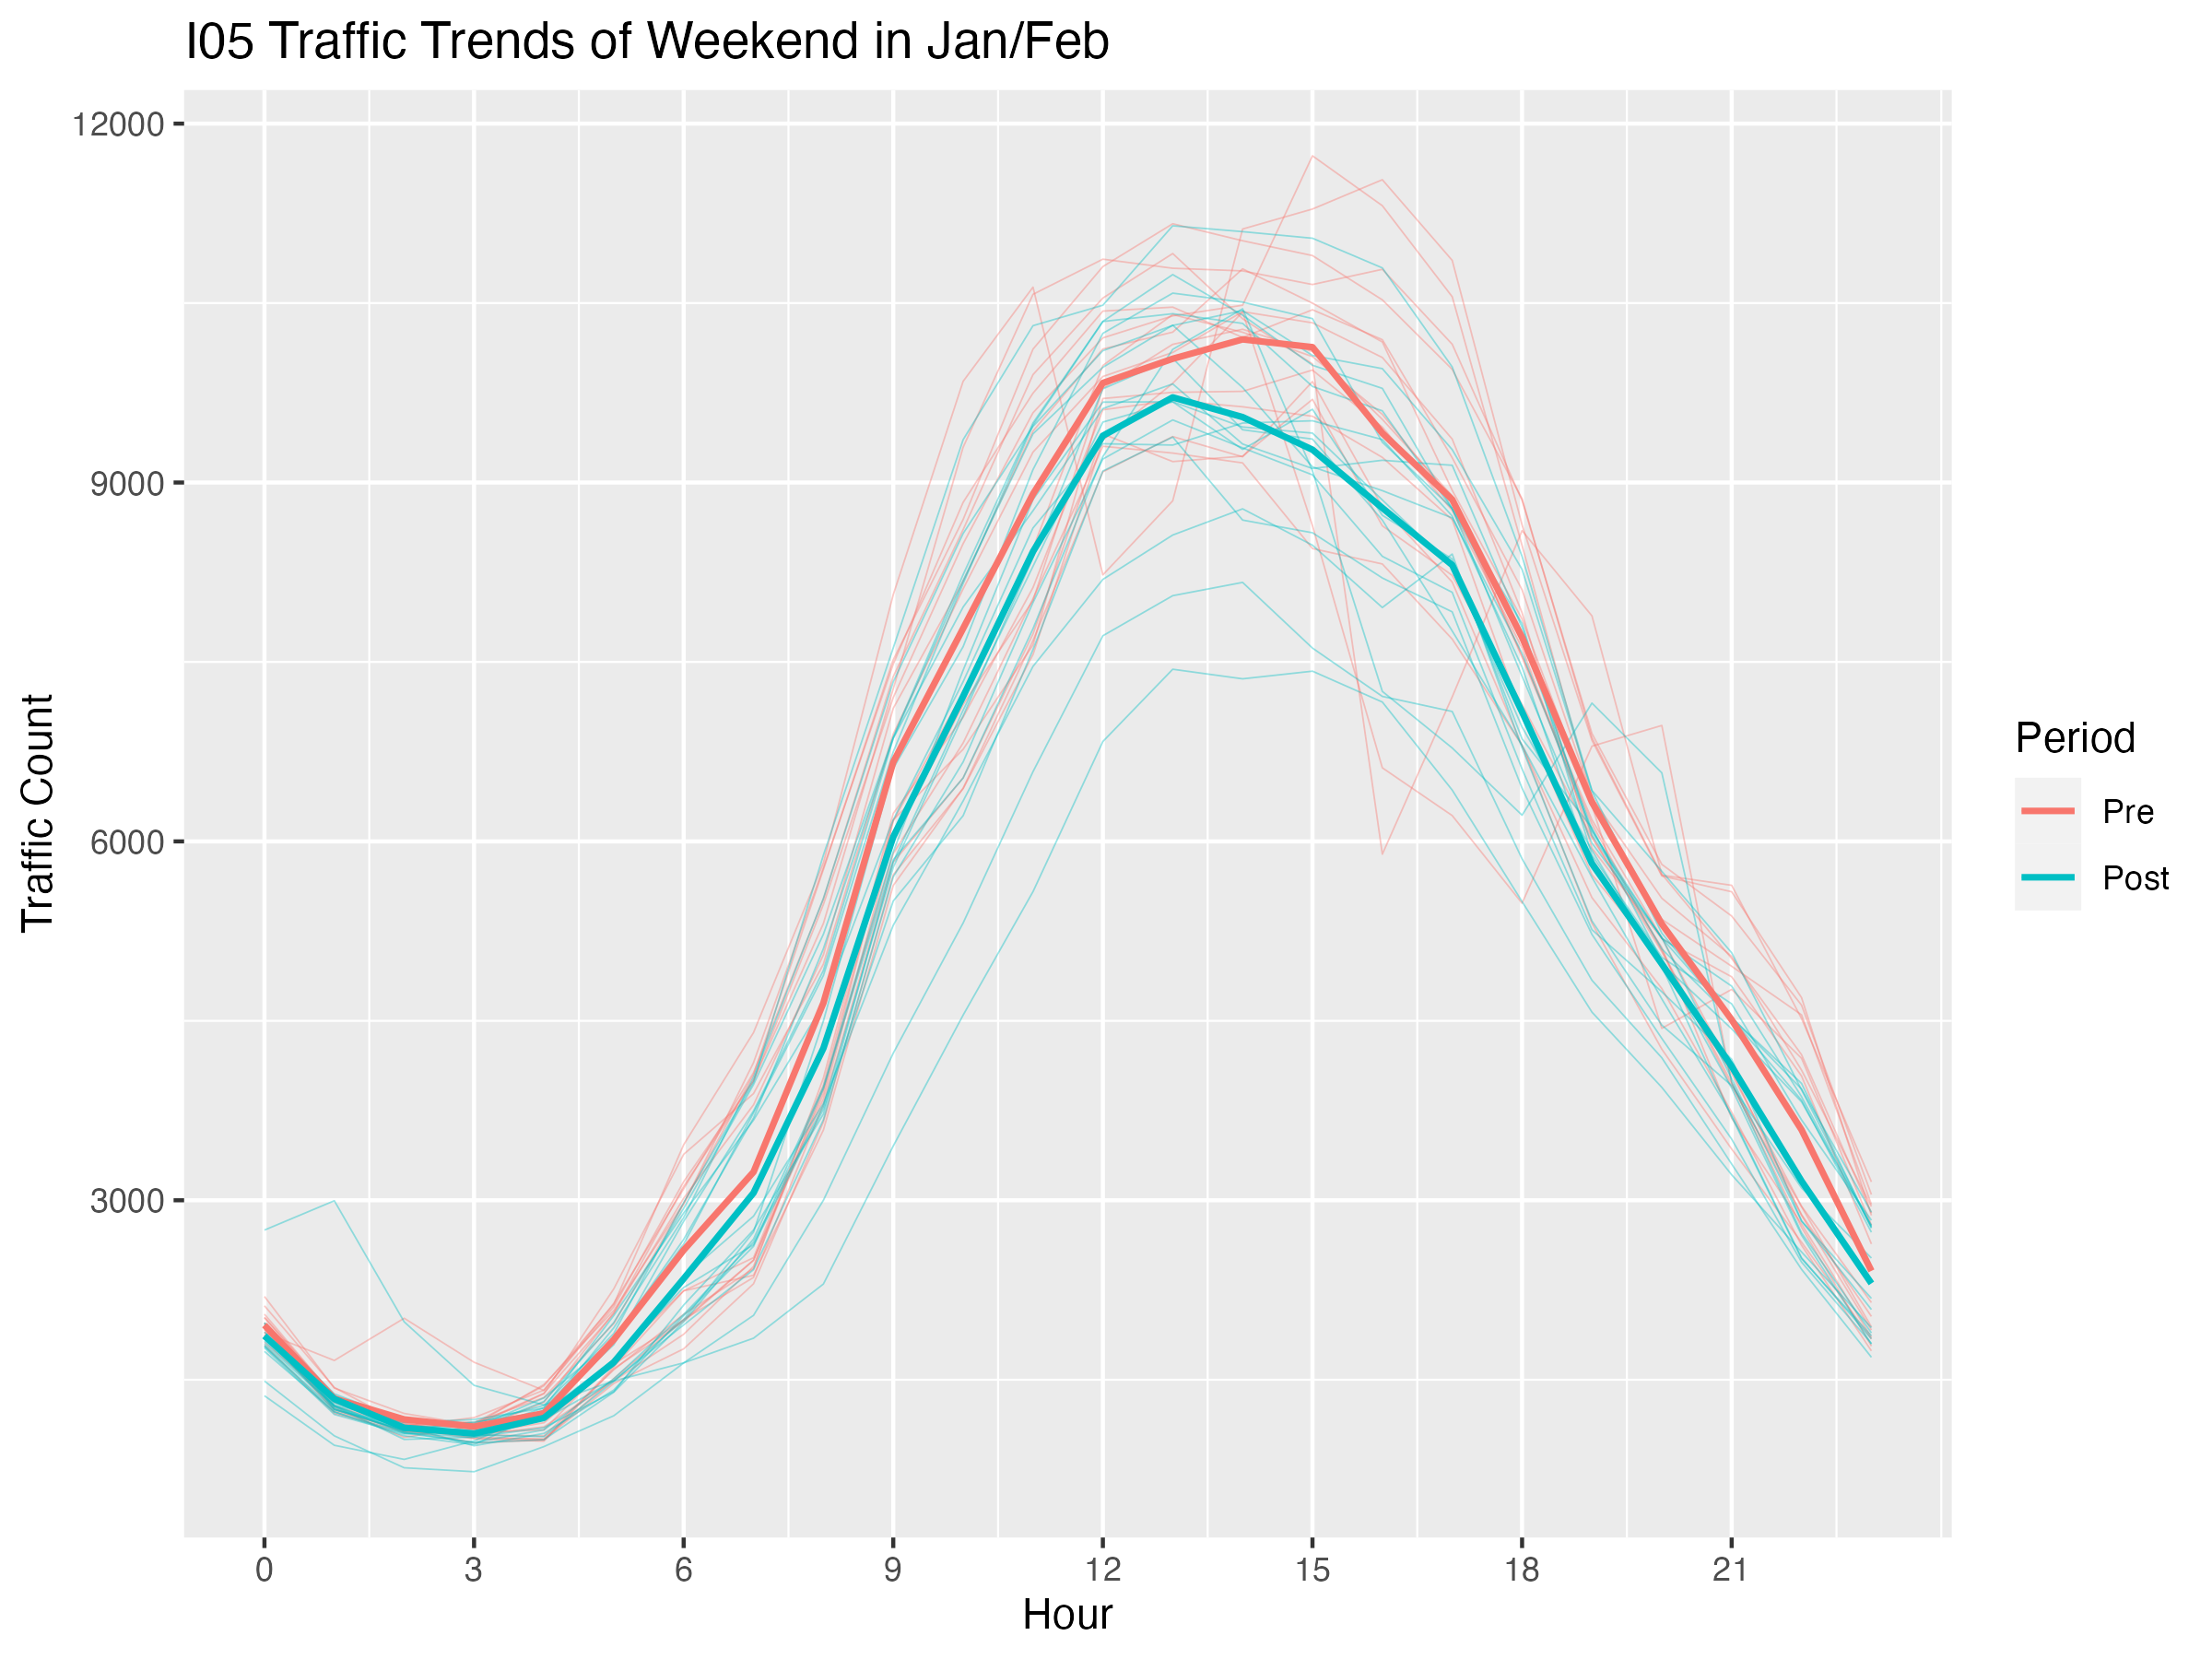
\includegraphics[width=\textwidth]{ATR26024_Plots/picture16_A24.png}
	\end{subfigure}
\end{figure}

\begin{figure}[H]
	\centering
	\begin{subfigure}[b]{0.45\textwidth}
		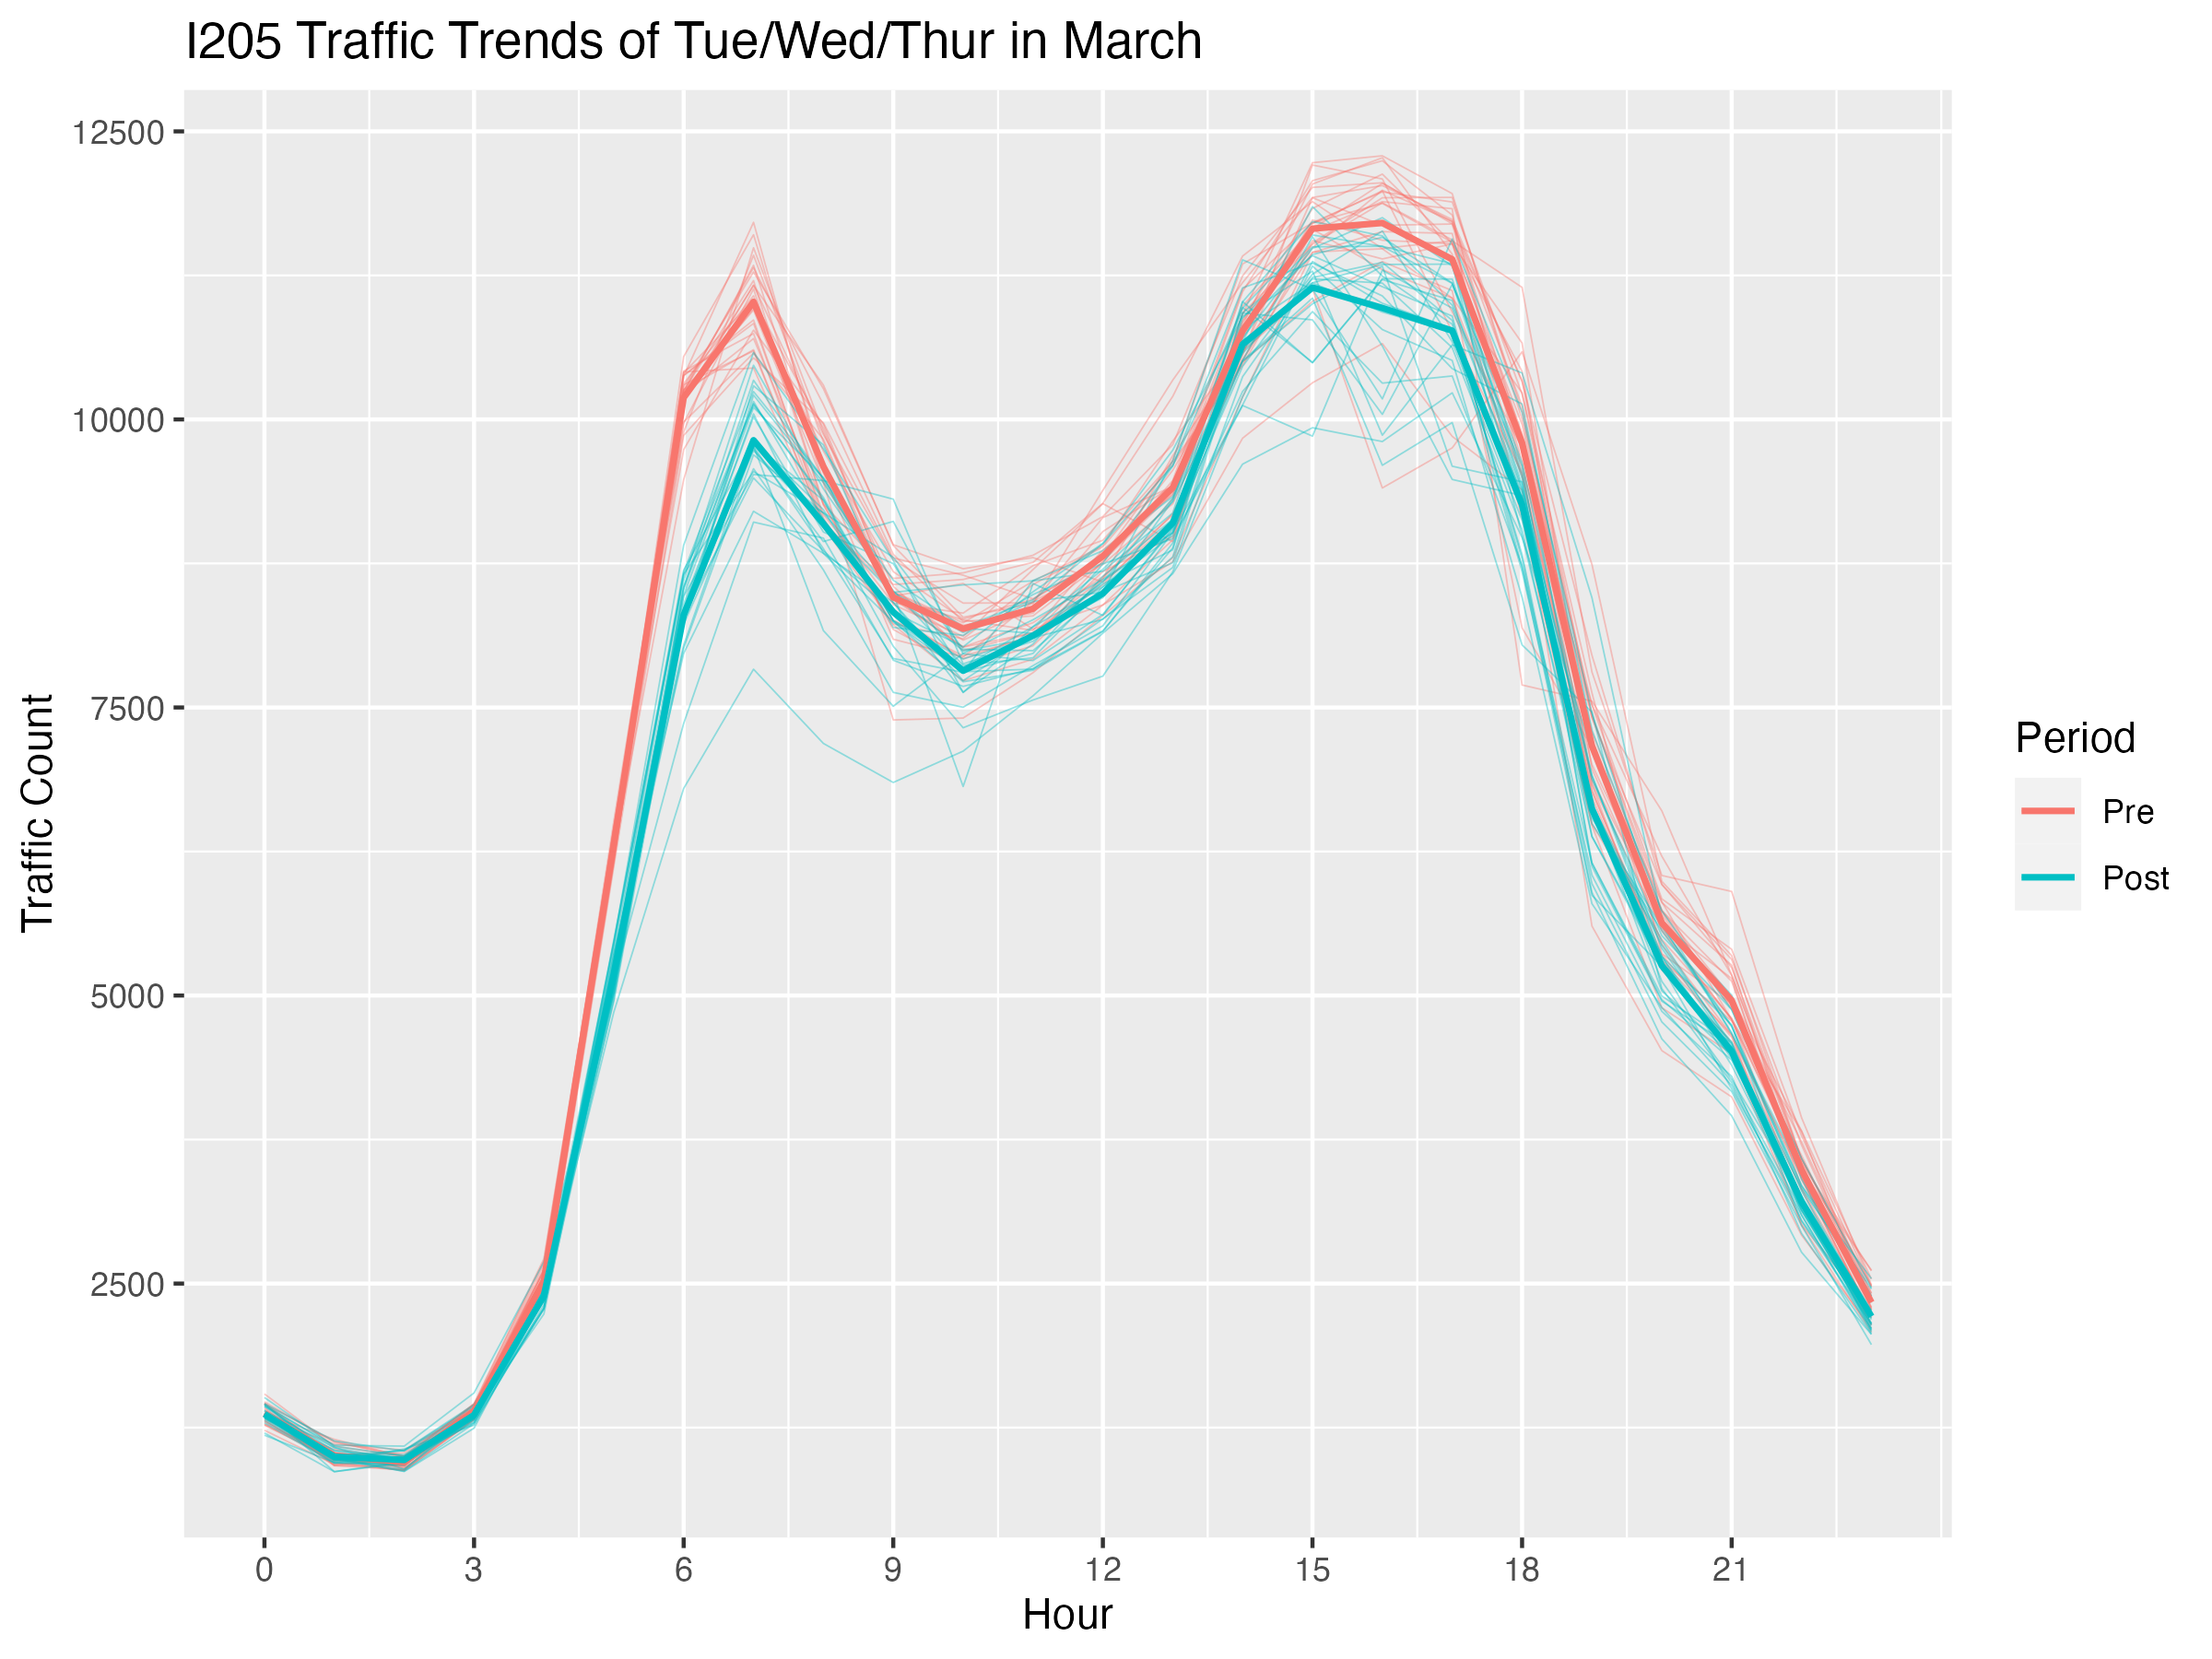
\includegraphics[width=\textwidth]{ATR26024_Plots/picture7_A24.png}
	\end{subfigure}
	\hfill
	\begin{subfigure}[b]{0.45\textwidth}
		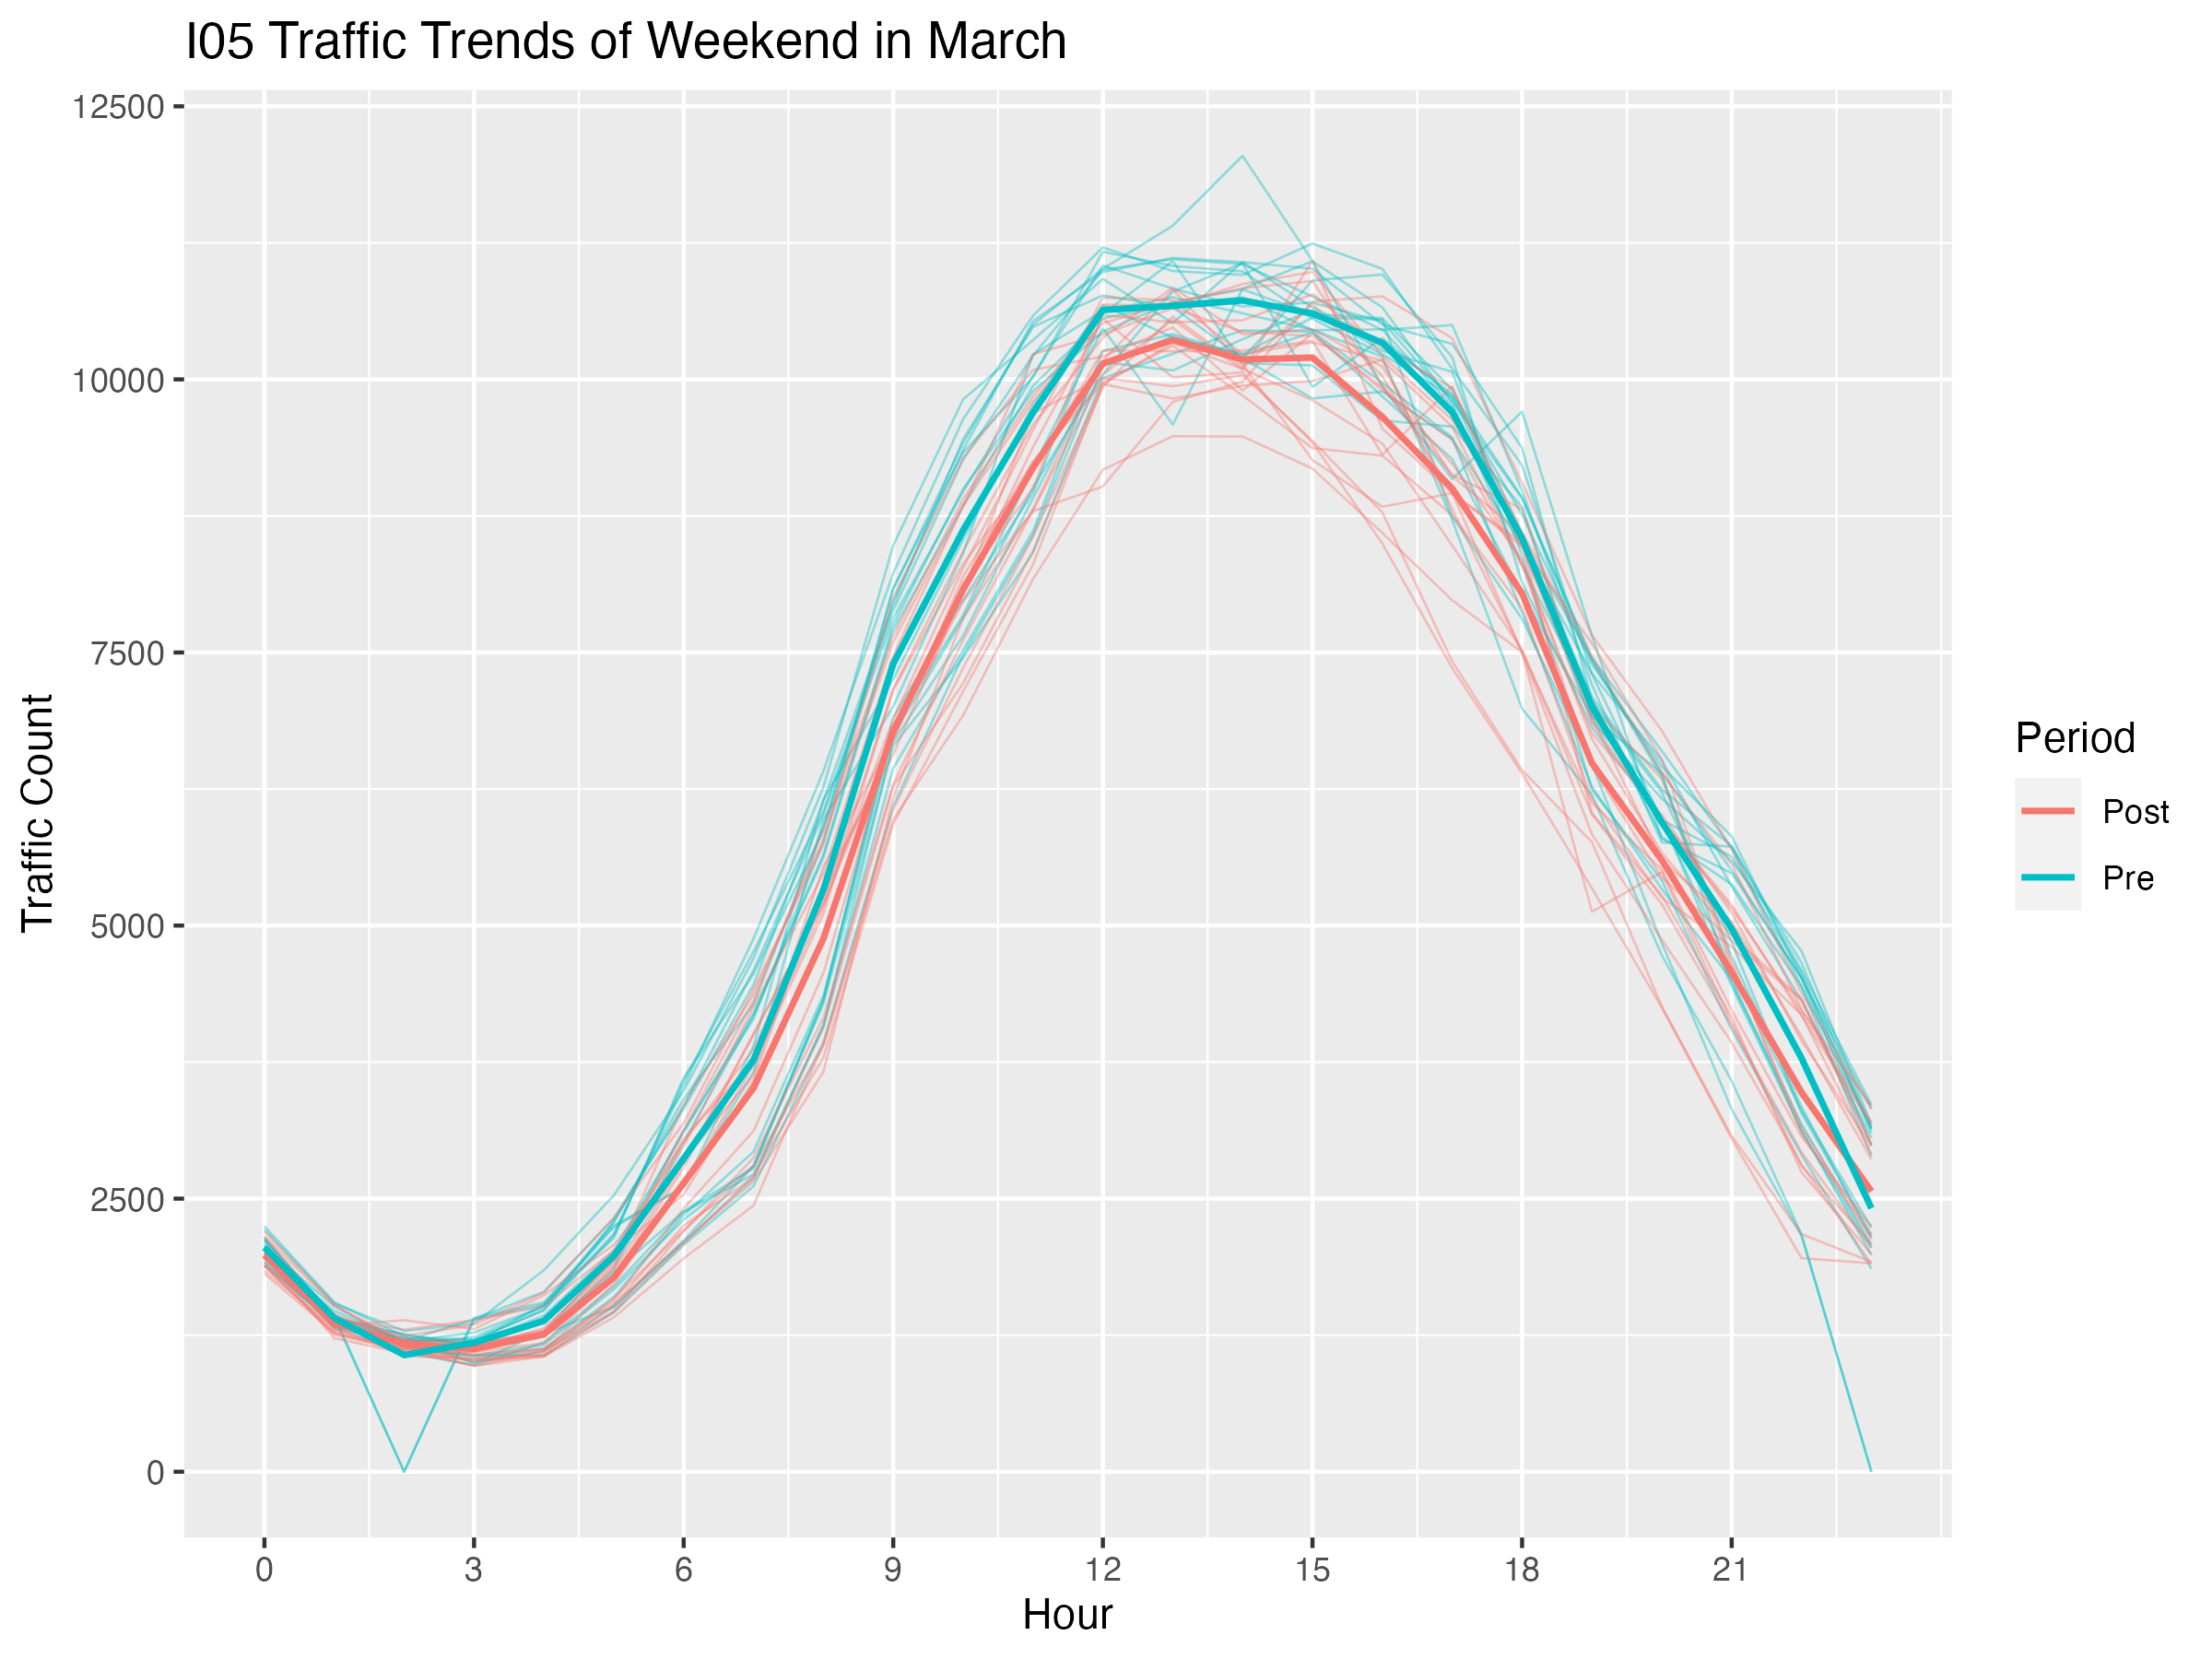
\includegraphics[width=\textwidth]{ATR26024_Plots/picture17_A24.png}
	\end{subfigure}
\end{figure}

\begin{figure}[H]
	\centering
	\begin{subfigure}[b]{0.45\textwidth}
		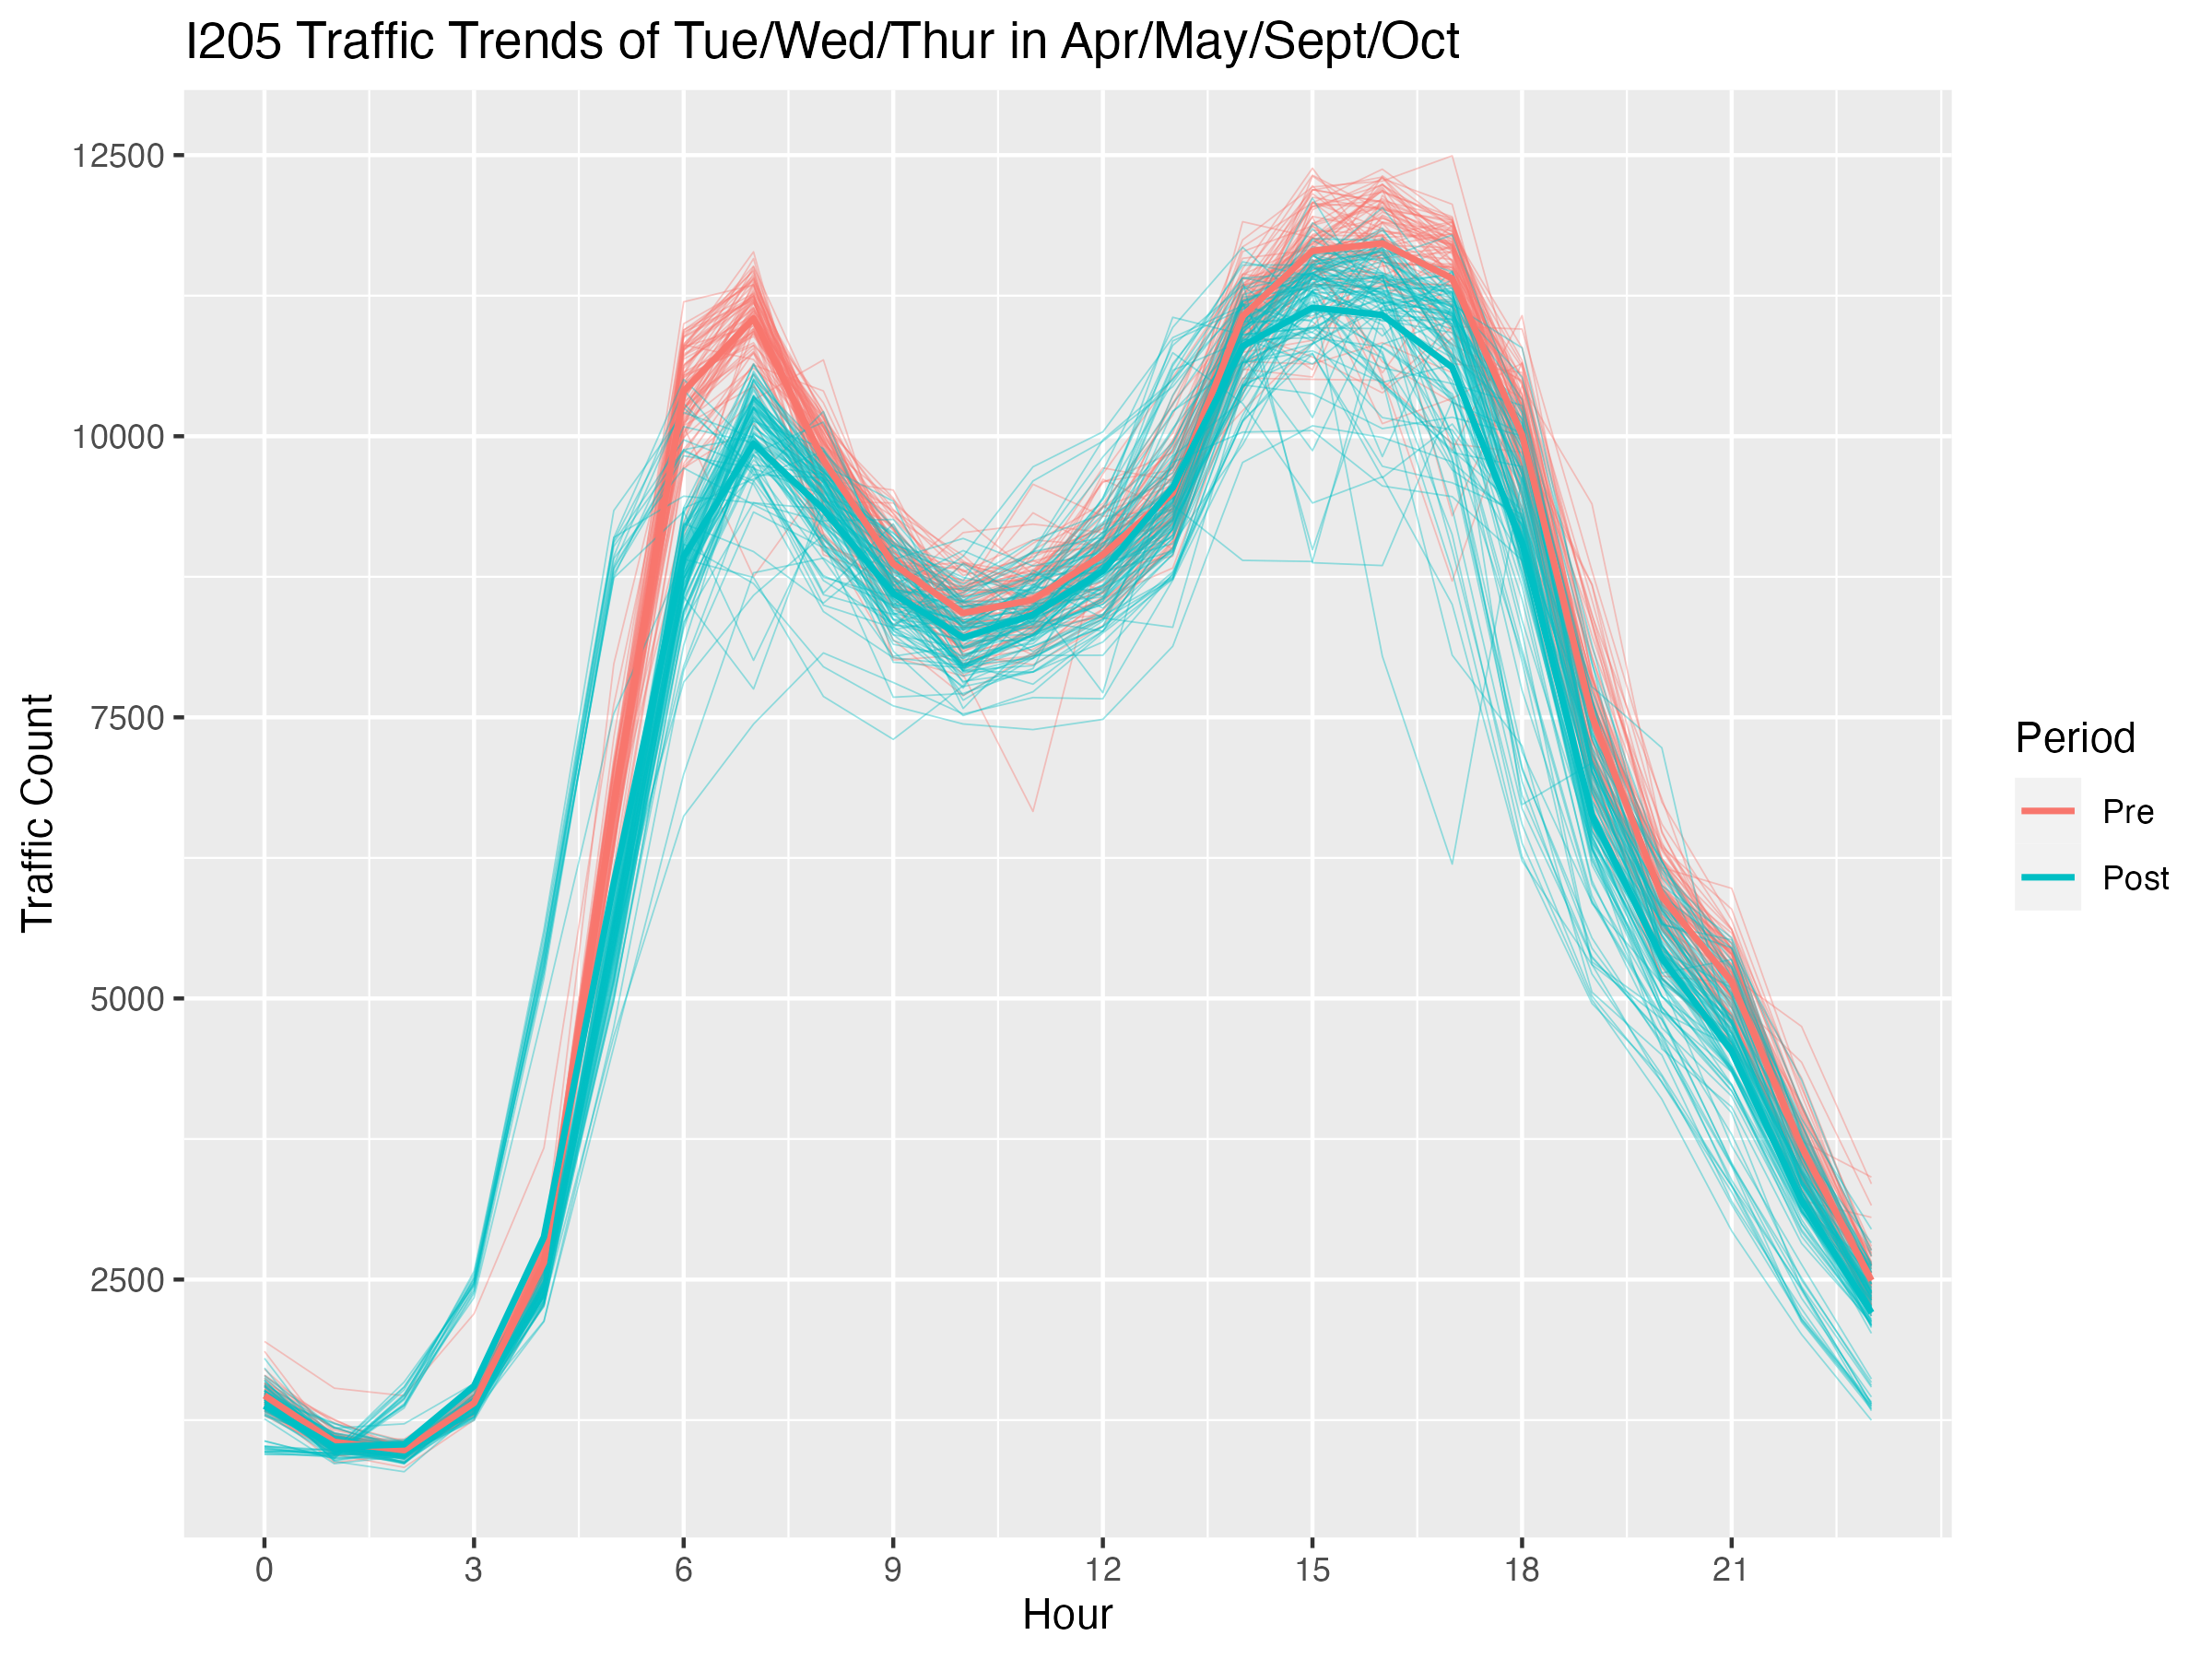
\includegraphics[width=\textwidth]{ATR26024_Plots/picture8_A24.png}
	\end{subfigure}
	\hfill
	\begin{subfigure}[b]{0.45\textwidth}
		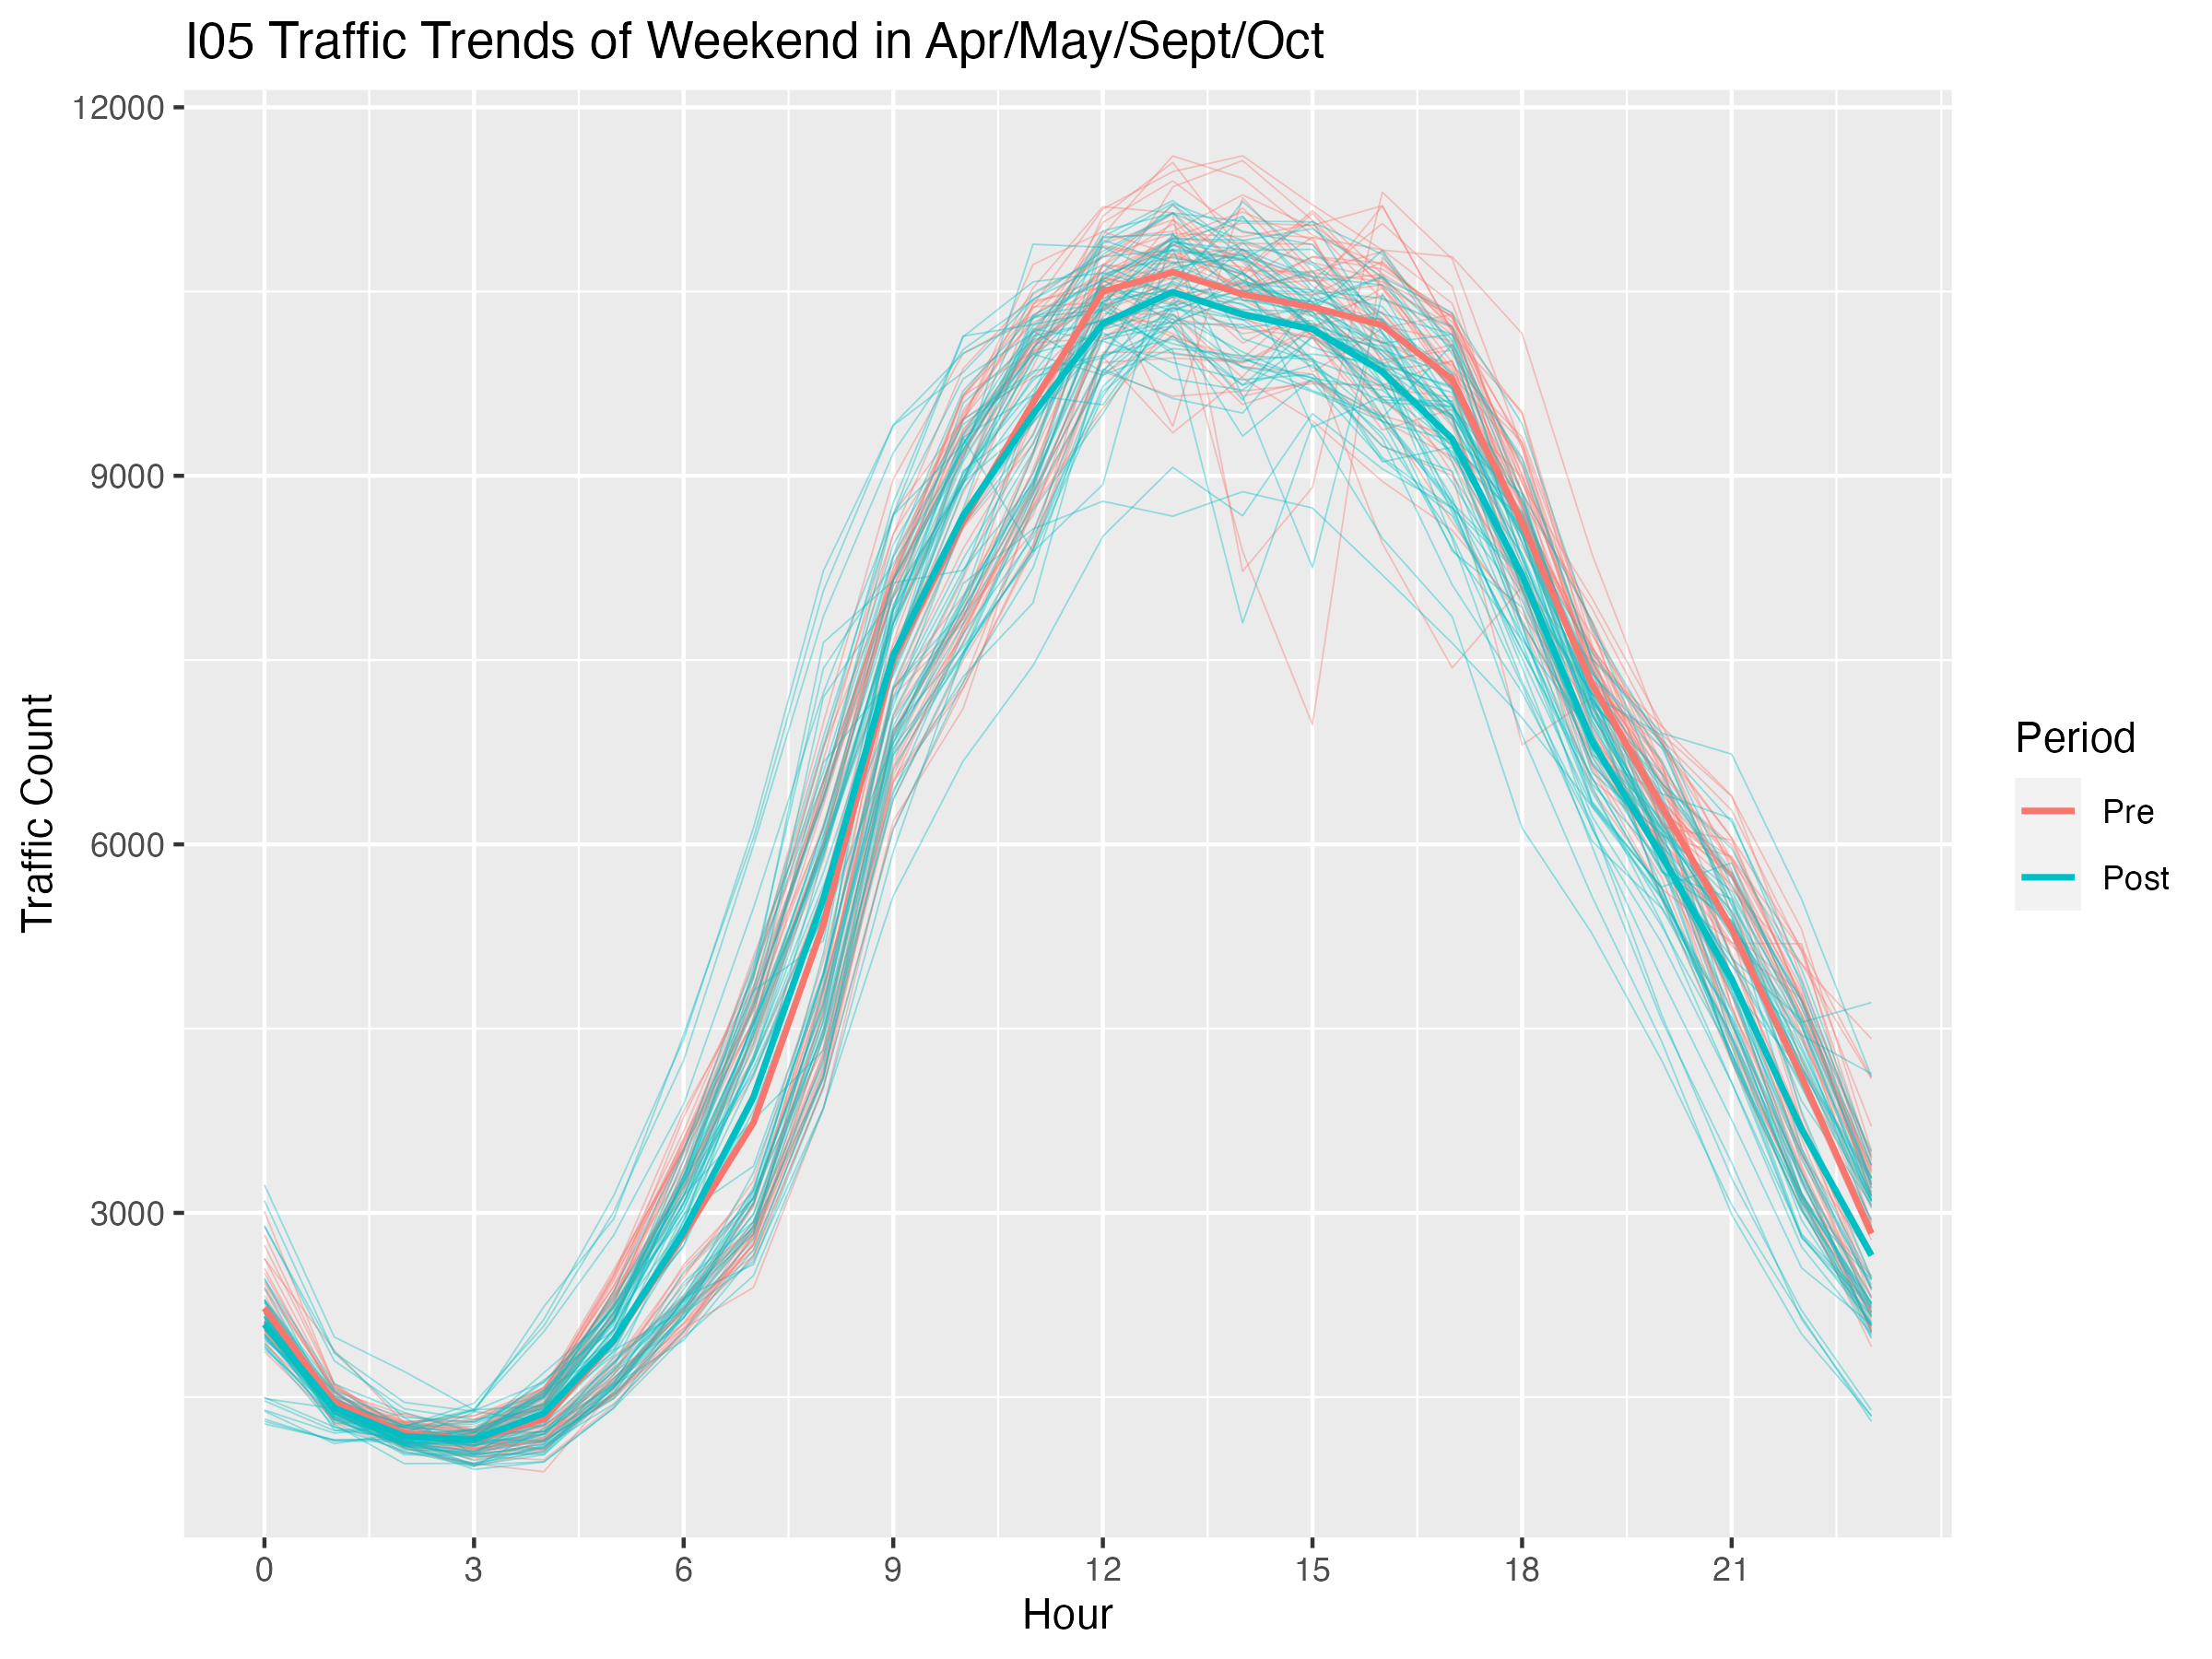
\includegraphics[width=\textwidth]{ATR26024_Plots/picture18_A24.png}
	\end{subfigure}
\end{figure}

\begin{figure}[H]
	\centering
	\begin{subfigure}[b]{0.45\textwidth}
		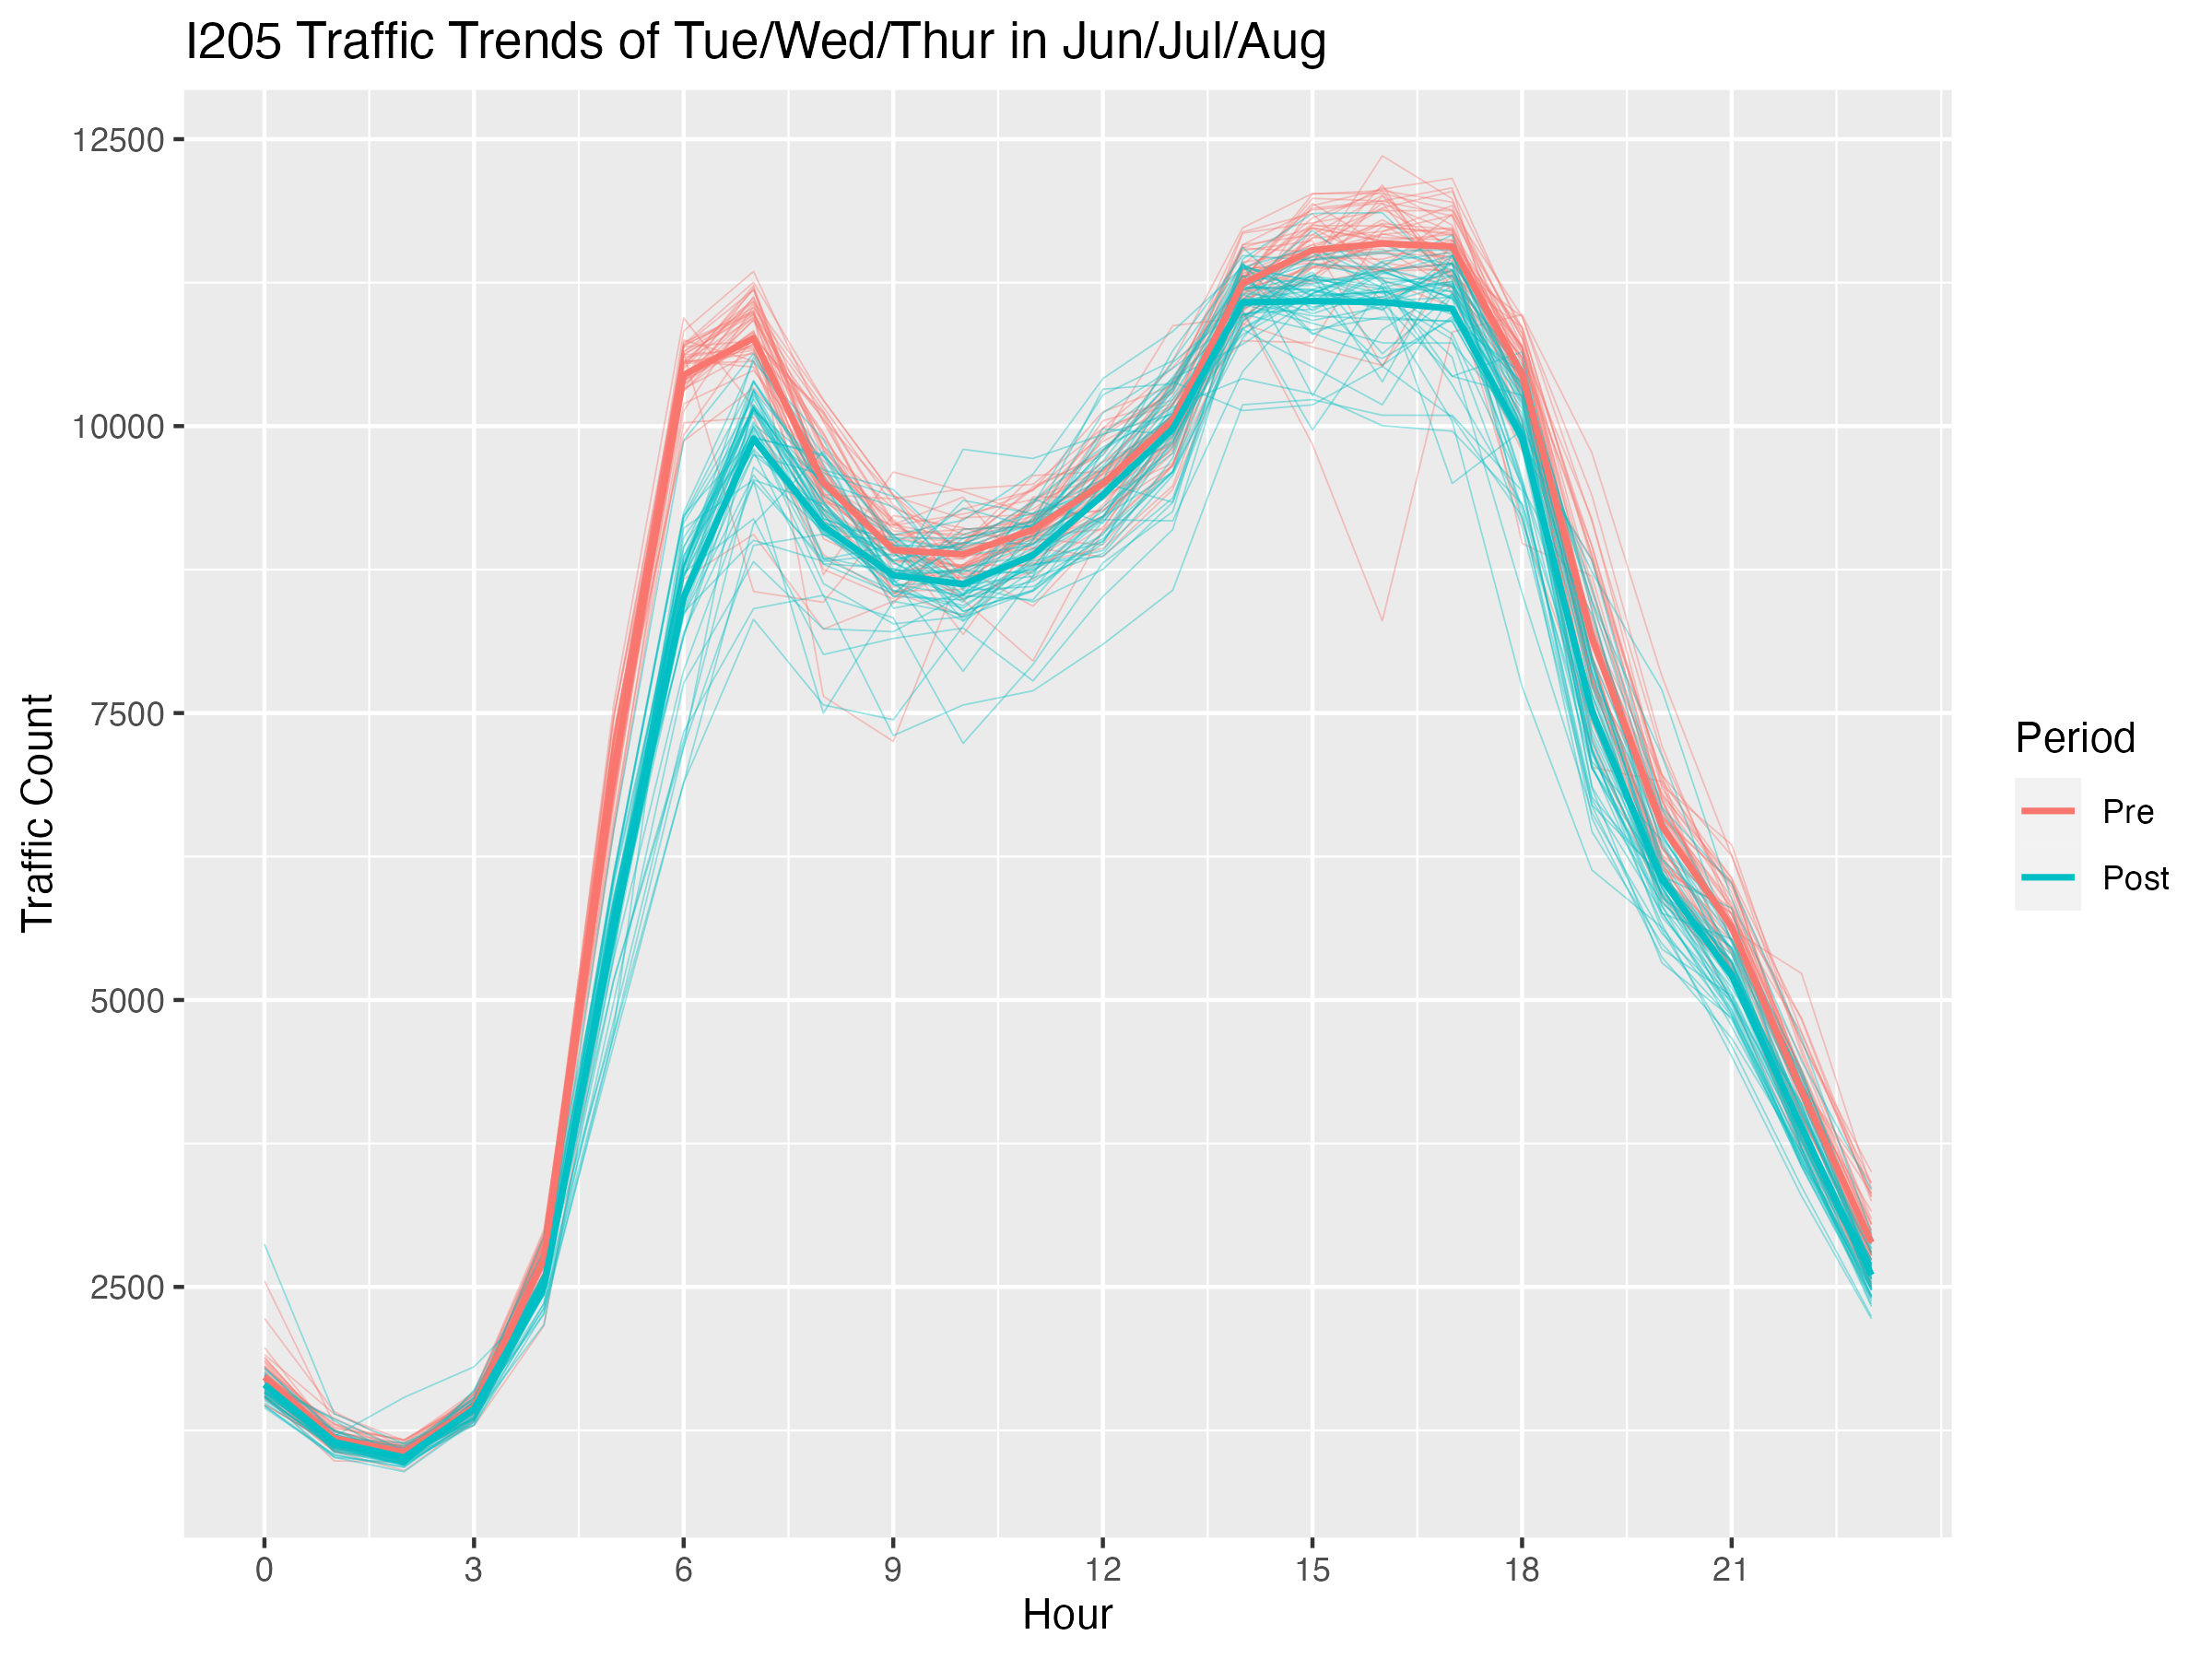
\includegraphics[width=\textwidth]{ATR26024_Plots/picture9_A24.png}
	\end{subfigure}
	\hfill
	\begin{subfigure}[b]{0.45\textwidth}
		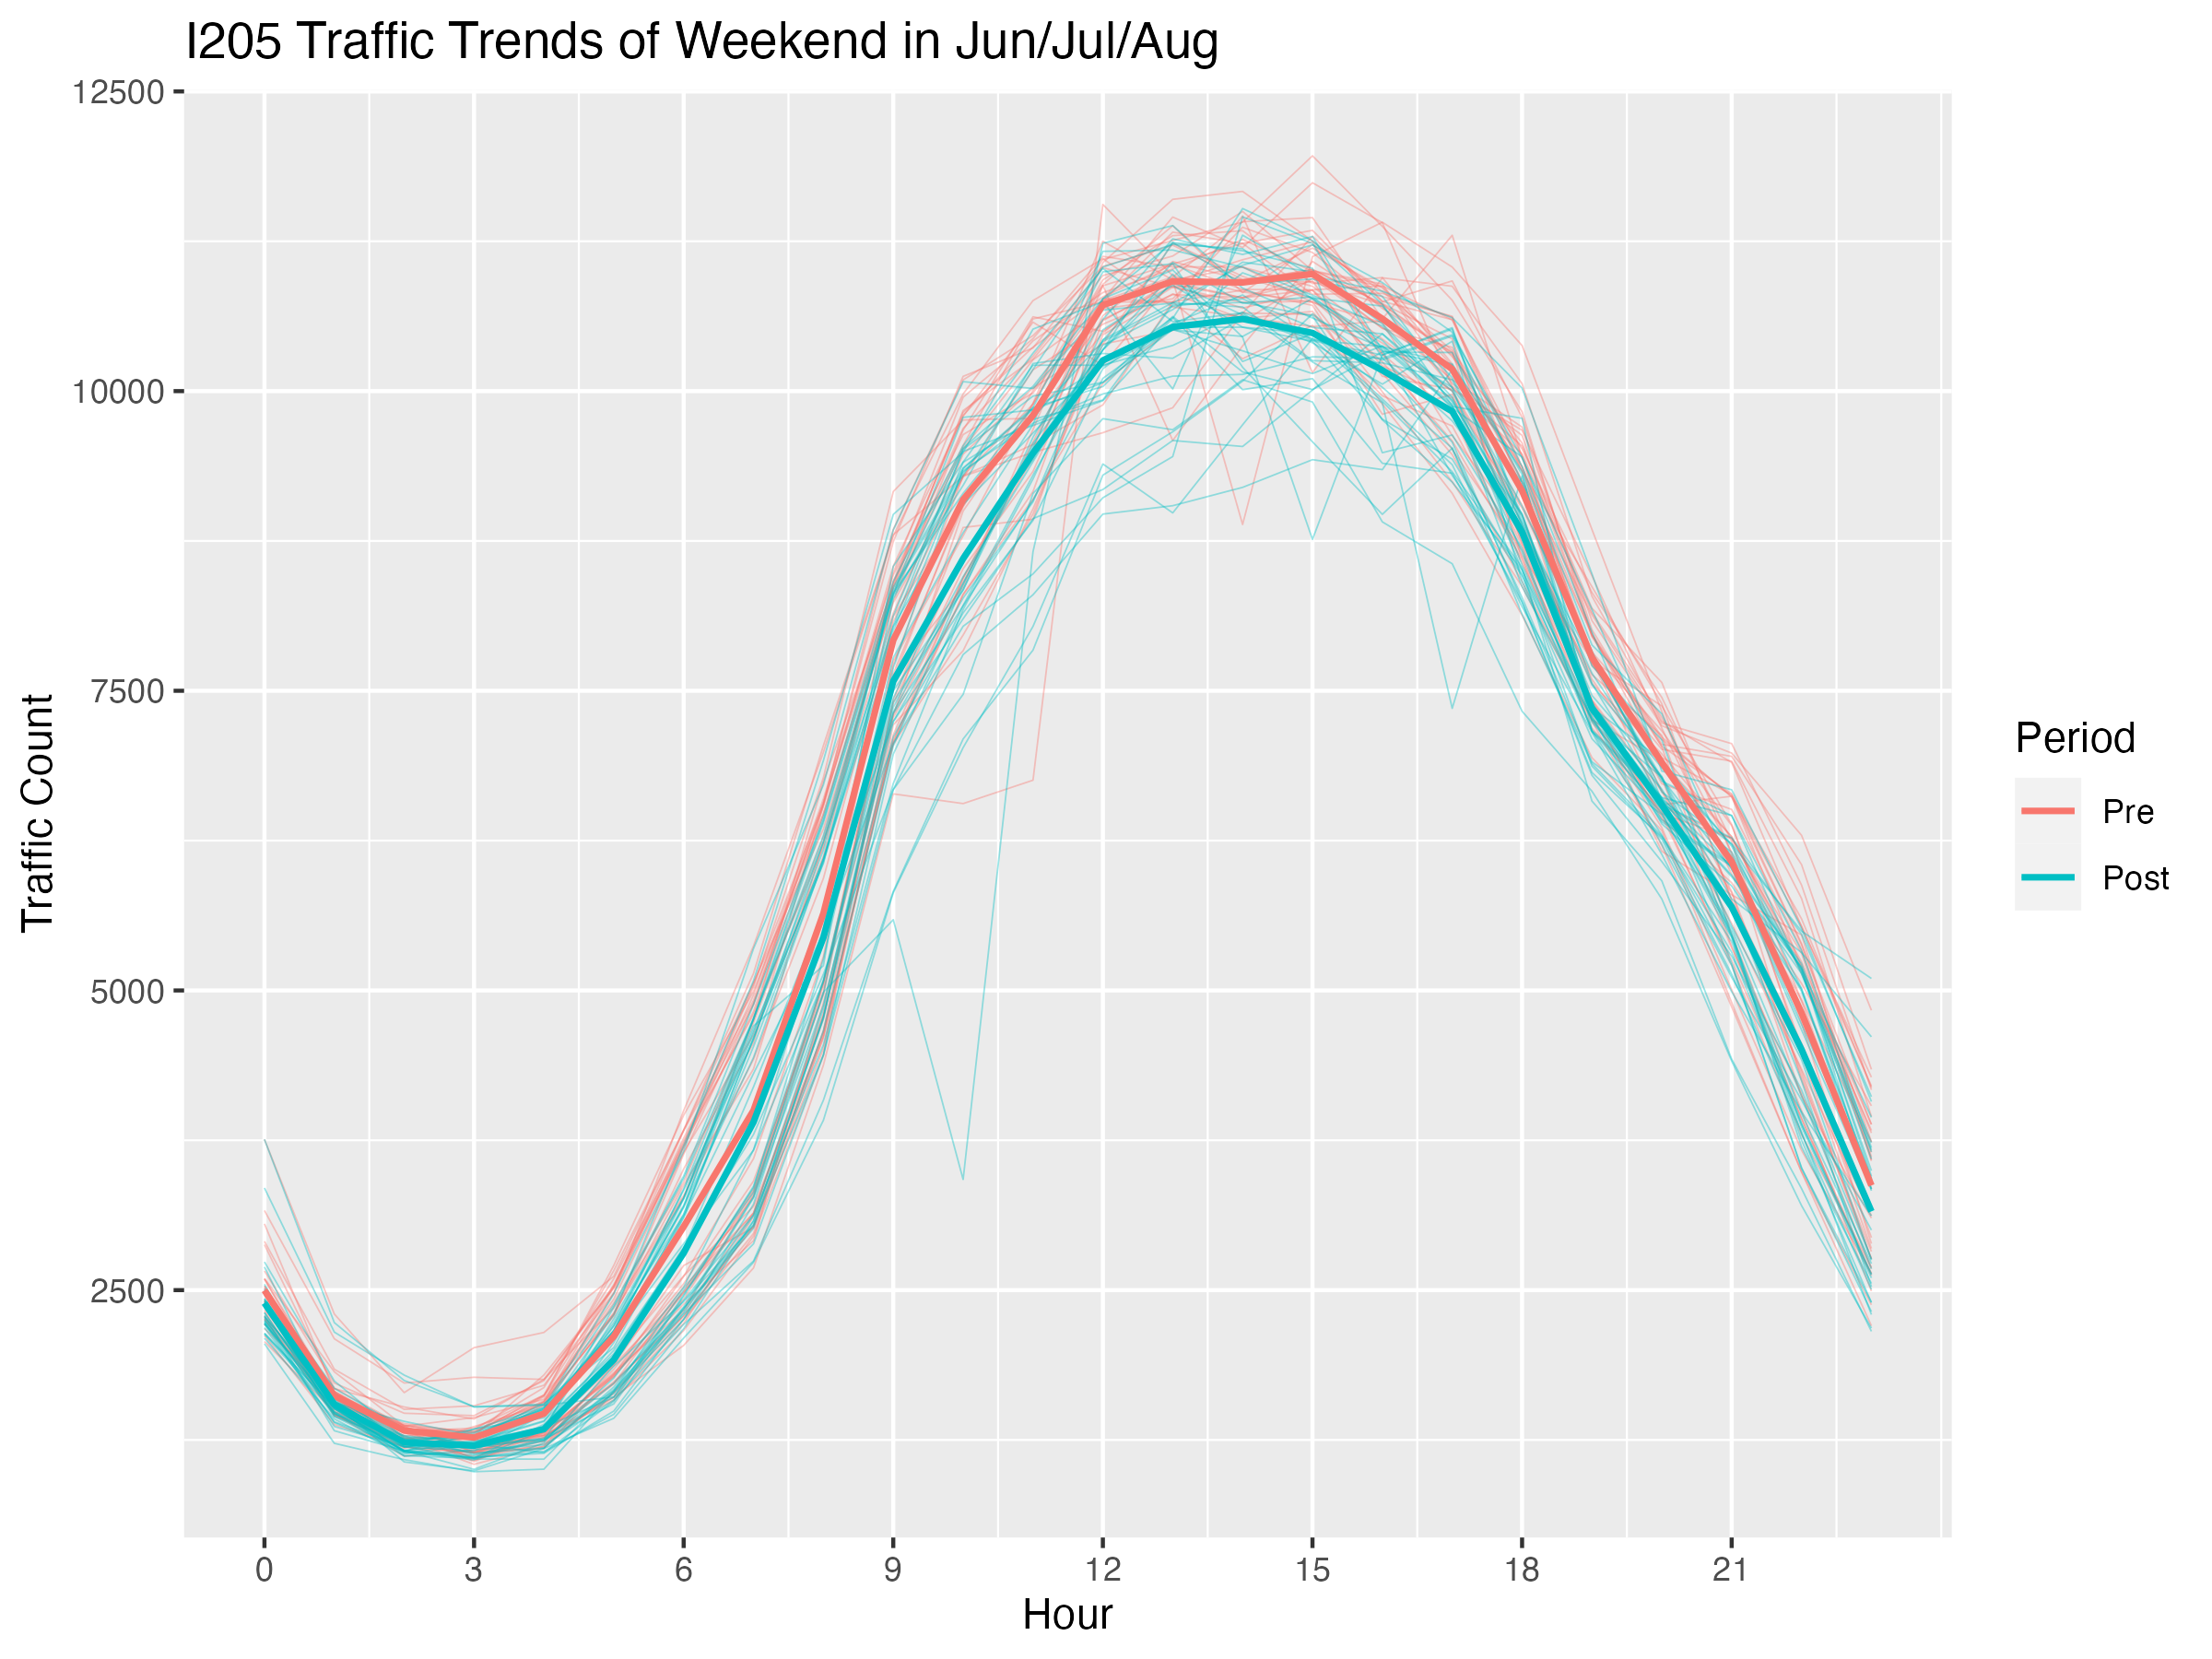
\includegraphics[width=\textwidth]{ATR26024_Plots/picture19_A24.png}
	\end{subfigure}
\end{figure}

\begin{figure}[H]
	\centering
	\begin{subfigure}[b]{0.45\textwidth}
		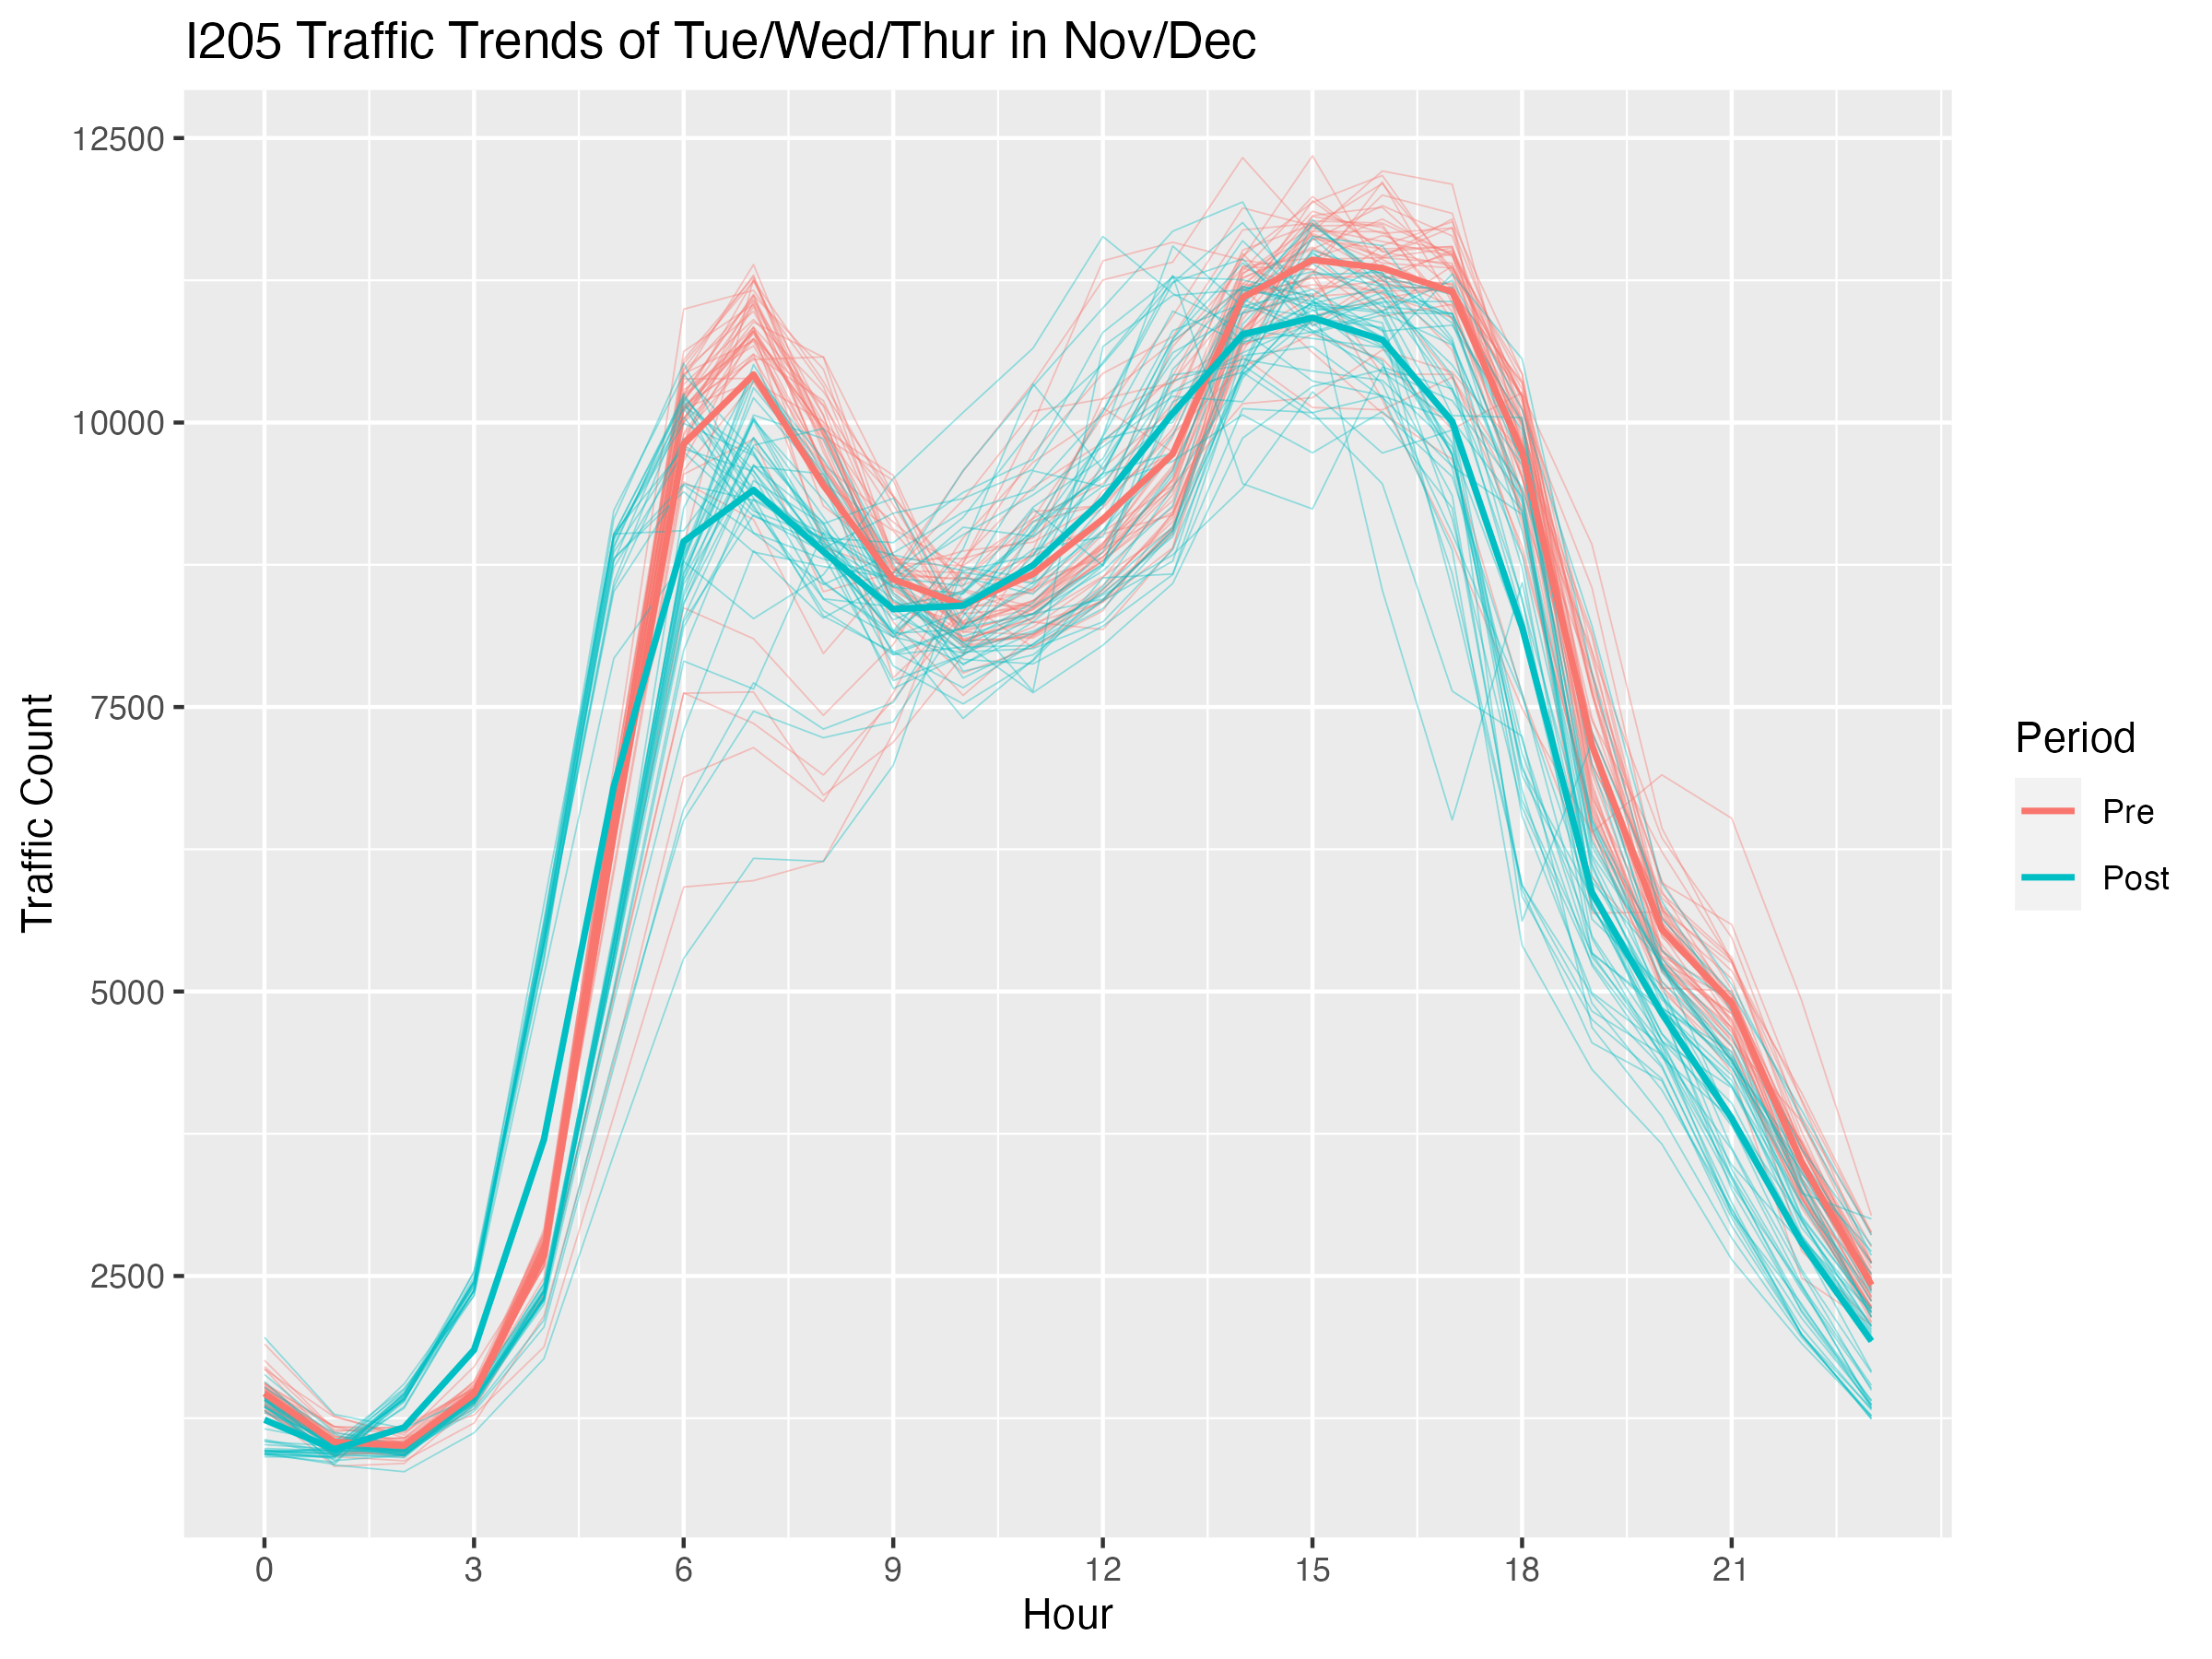
\includegraphics[width=\textwidth]{ATR26024_Plots/picture10_A24.png}
	\end{subfigure}
	\hfill
	\begin{subfigure}[b]{0.45\textwidth}
		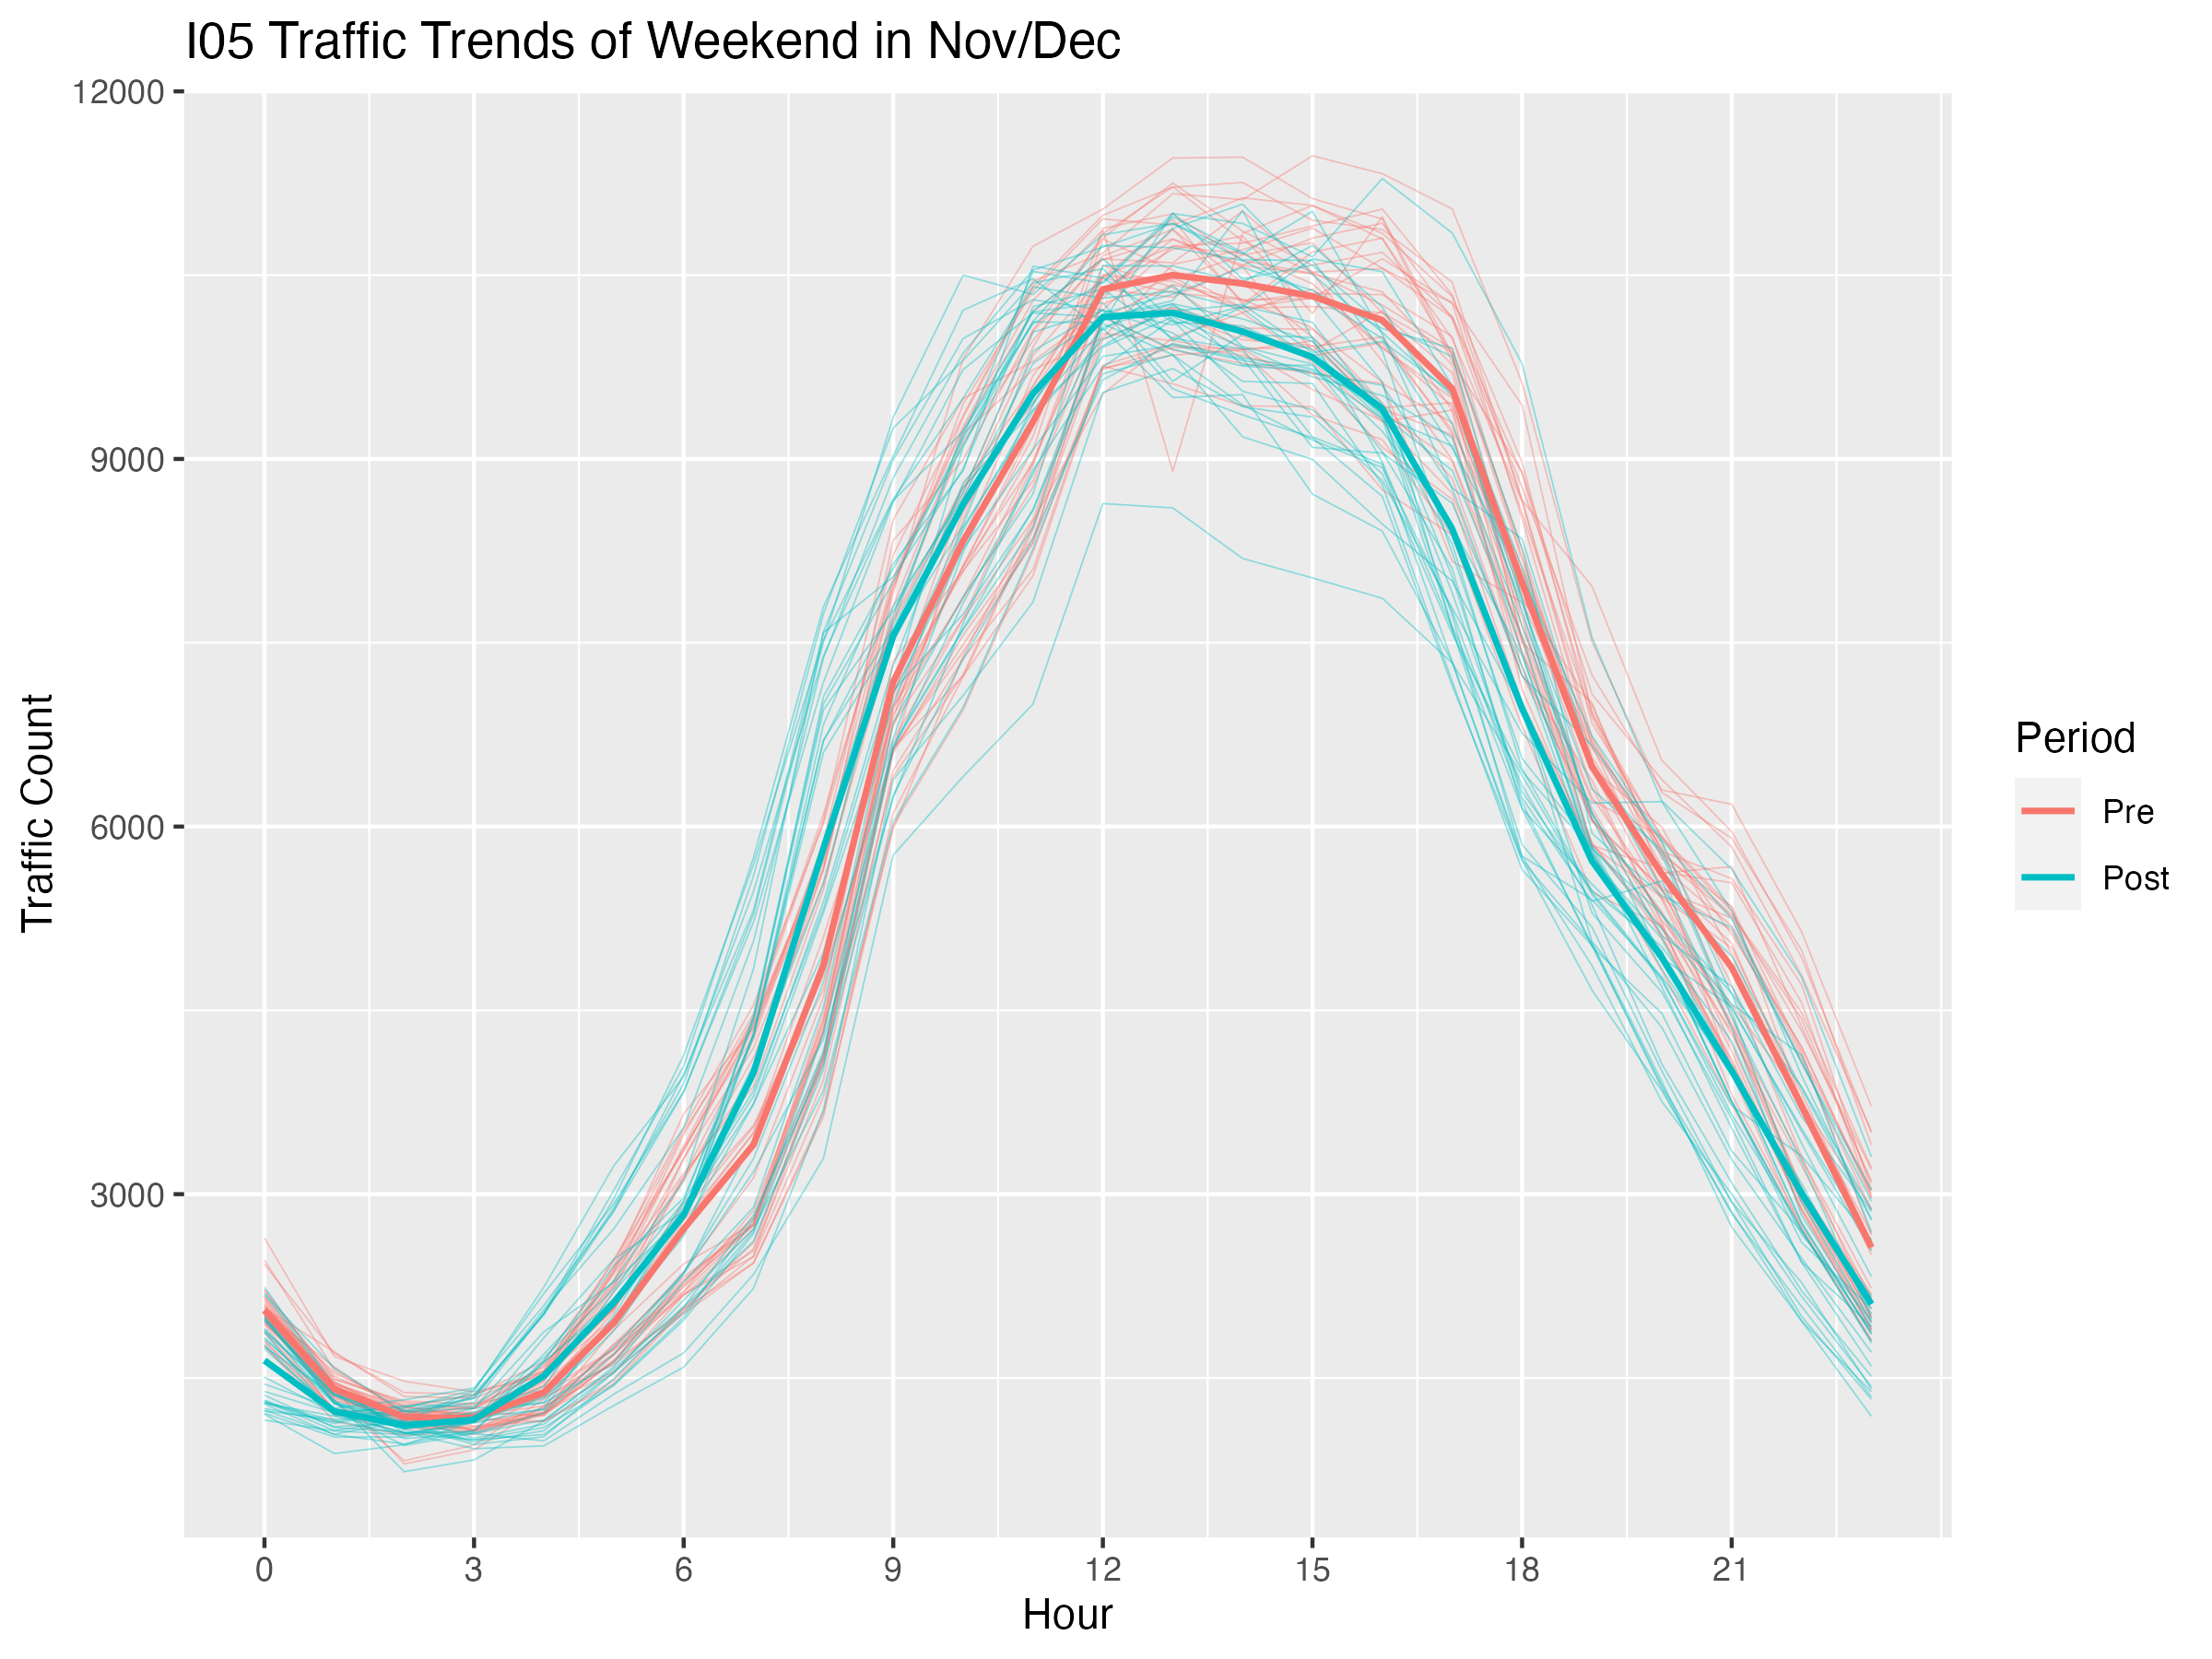
\includegraphics[width=\textwidth]{ATR26024_Plots/picture20_A24.png}
	\end{subfigure}
\end{figure}


\section{MMD P-Values}

\begin{figure}[H] 
    \centering
    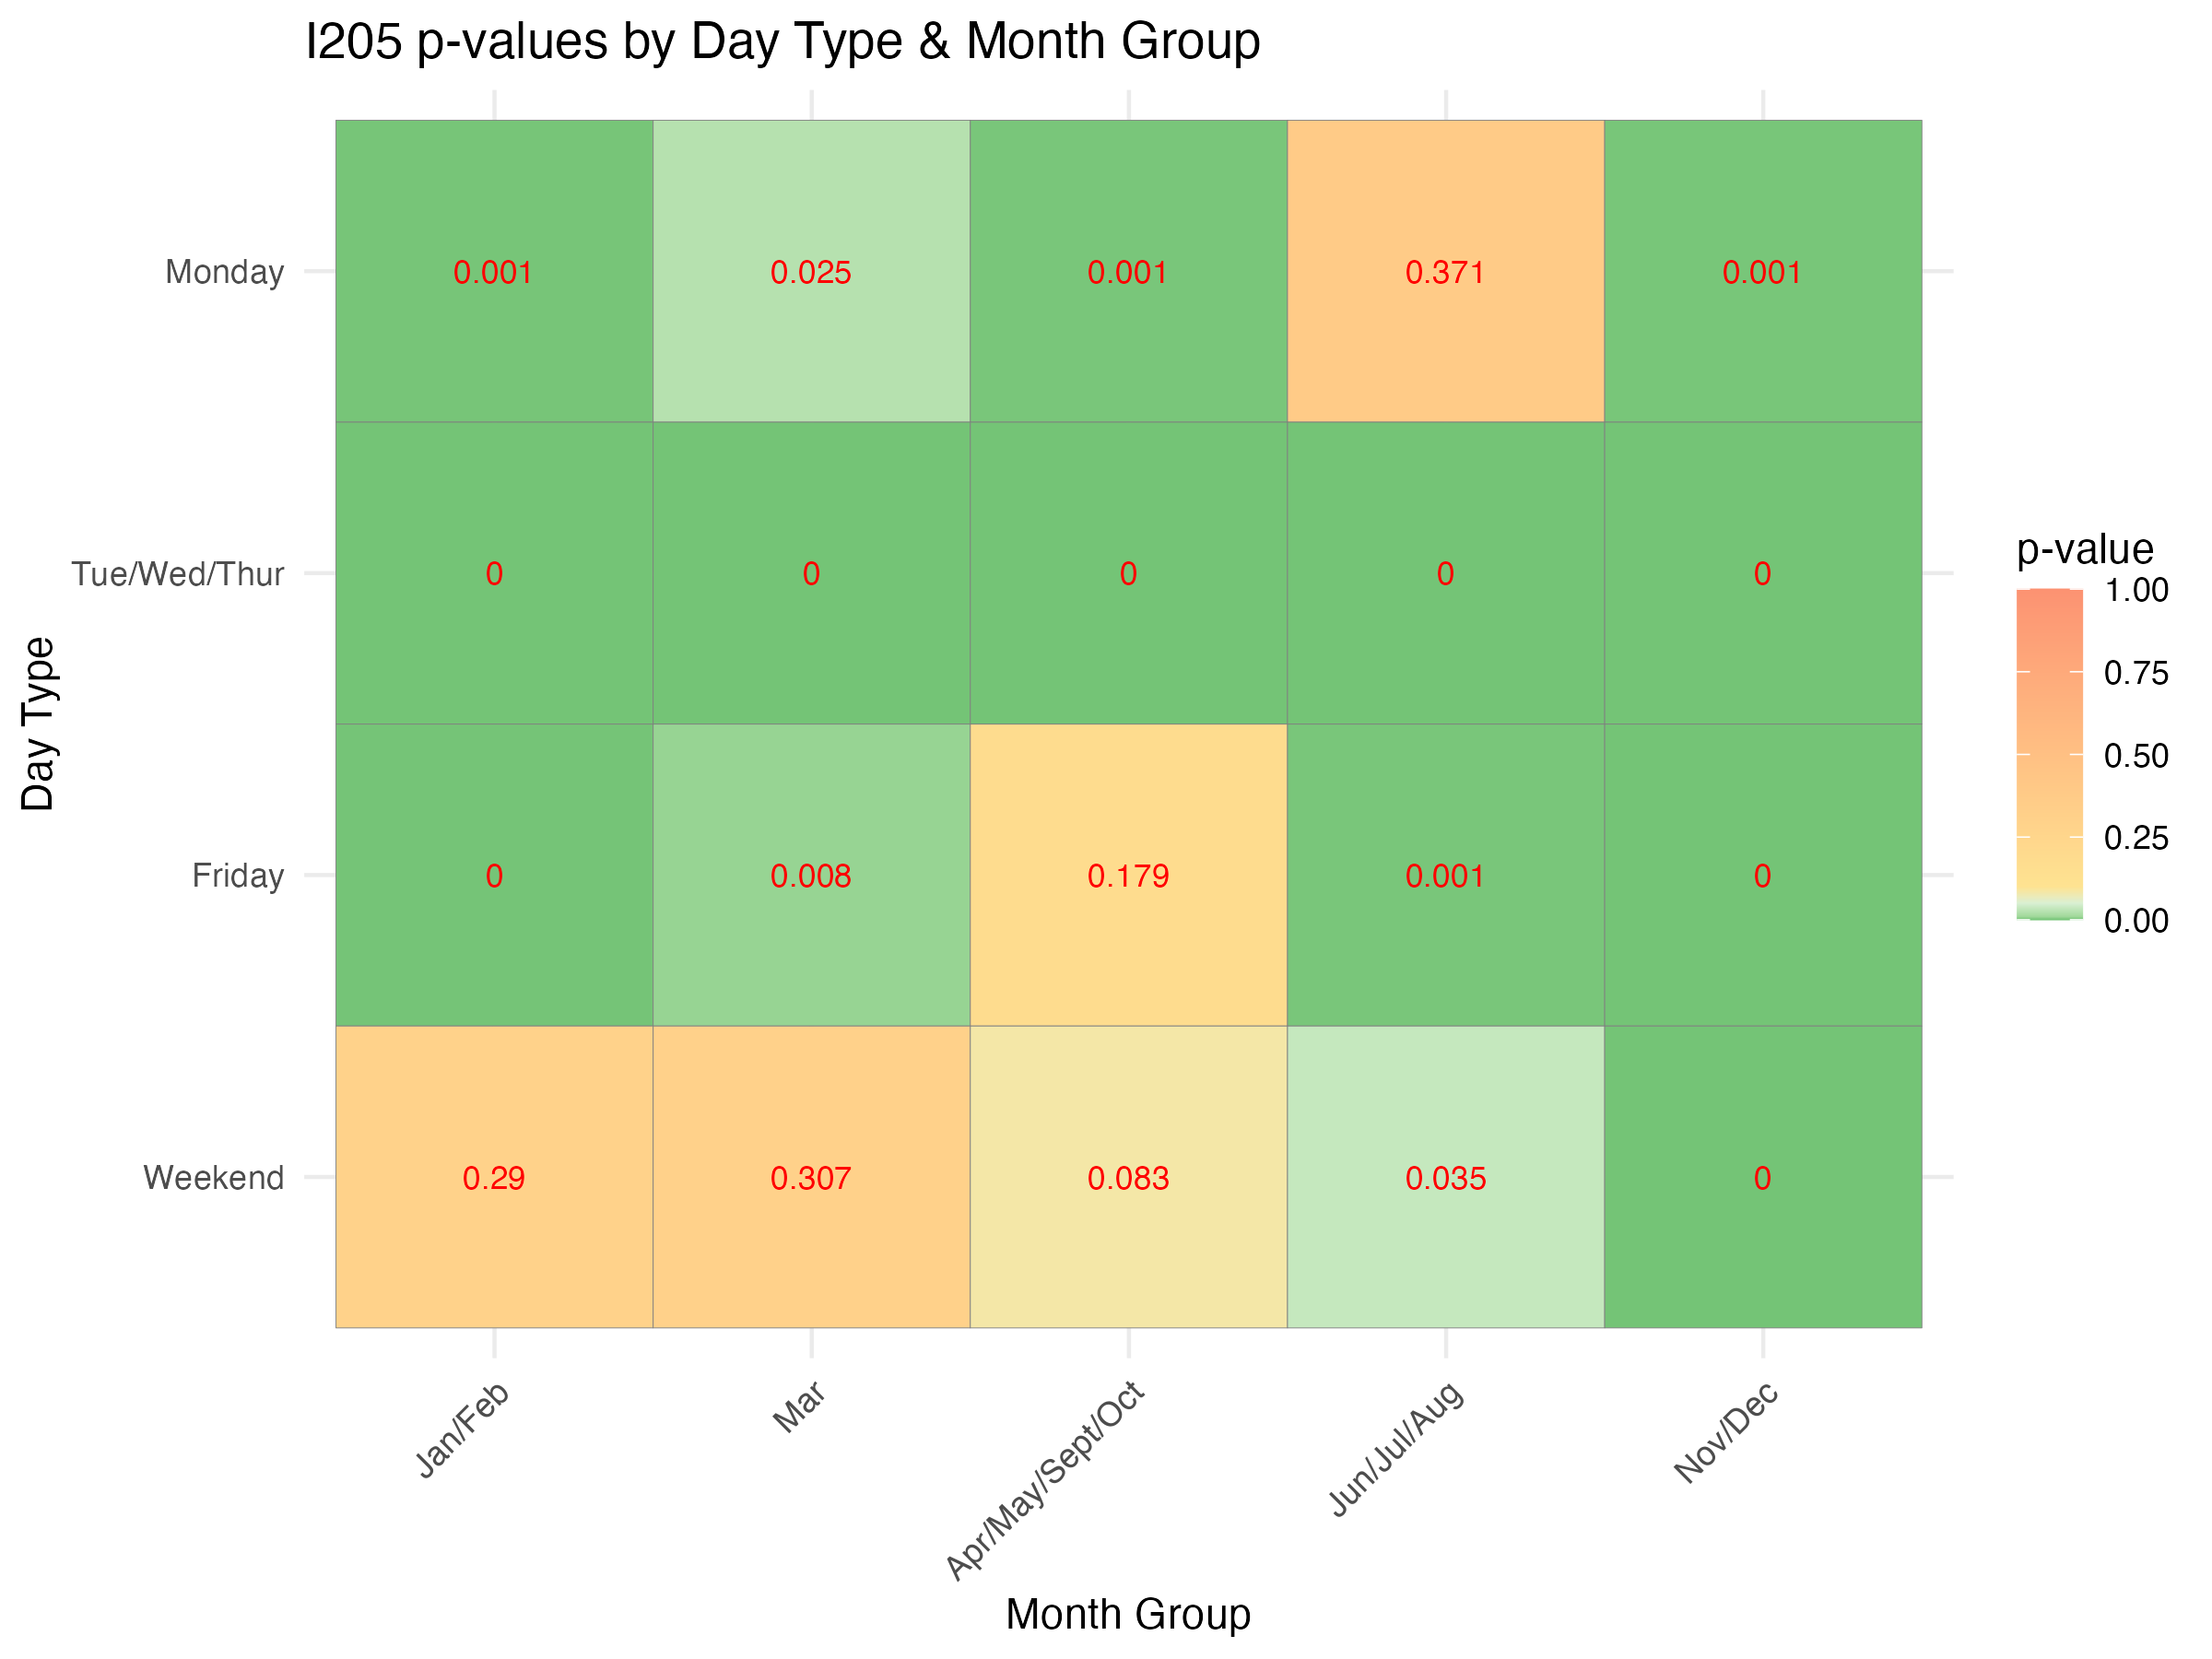
\includegraphics[width=0.75\textwidth]{ATR26024_Plots/pvalues_A24.png}
    \label{fig:i205_pvalues}
\end{figure}

\begin{figure}[H] 
    \centering
    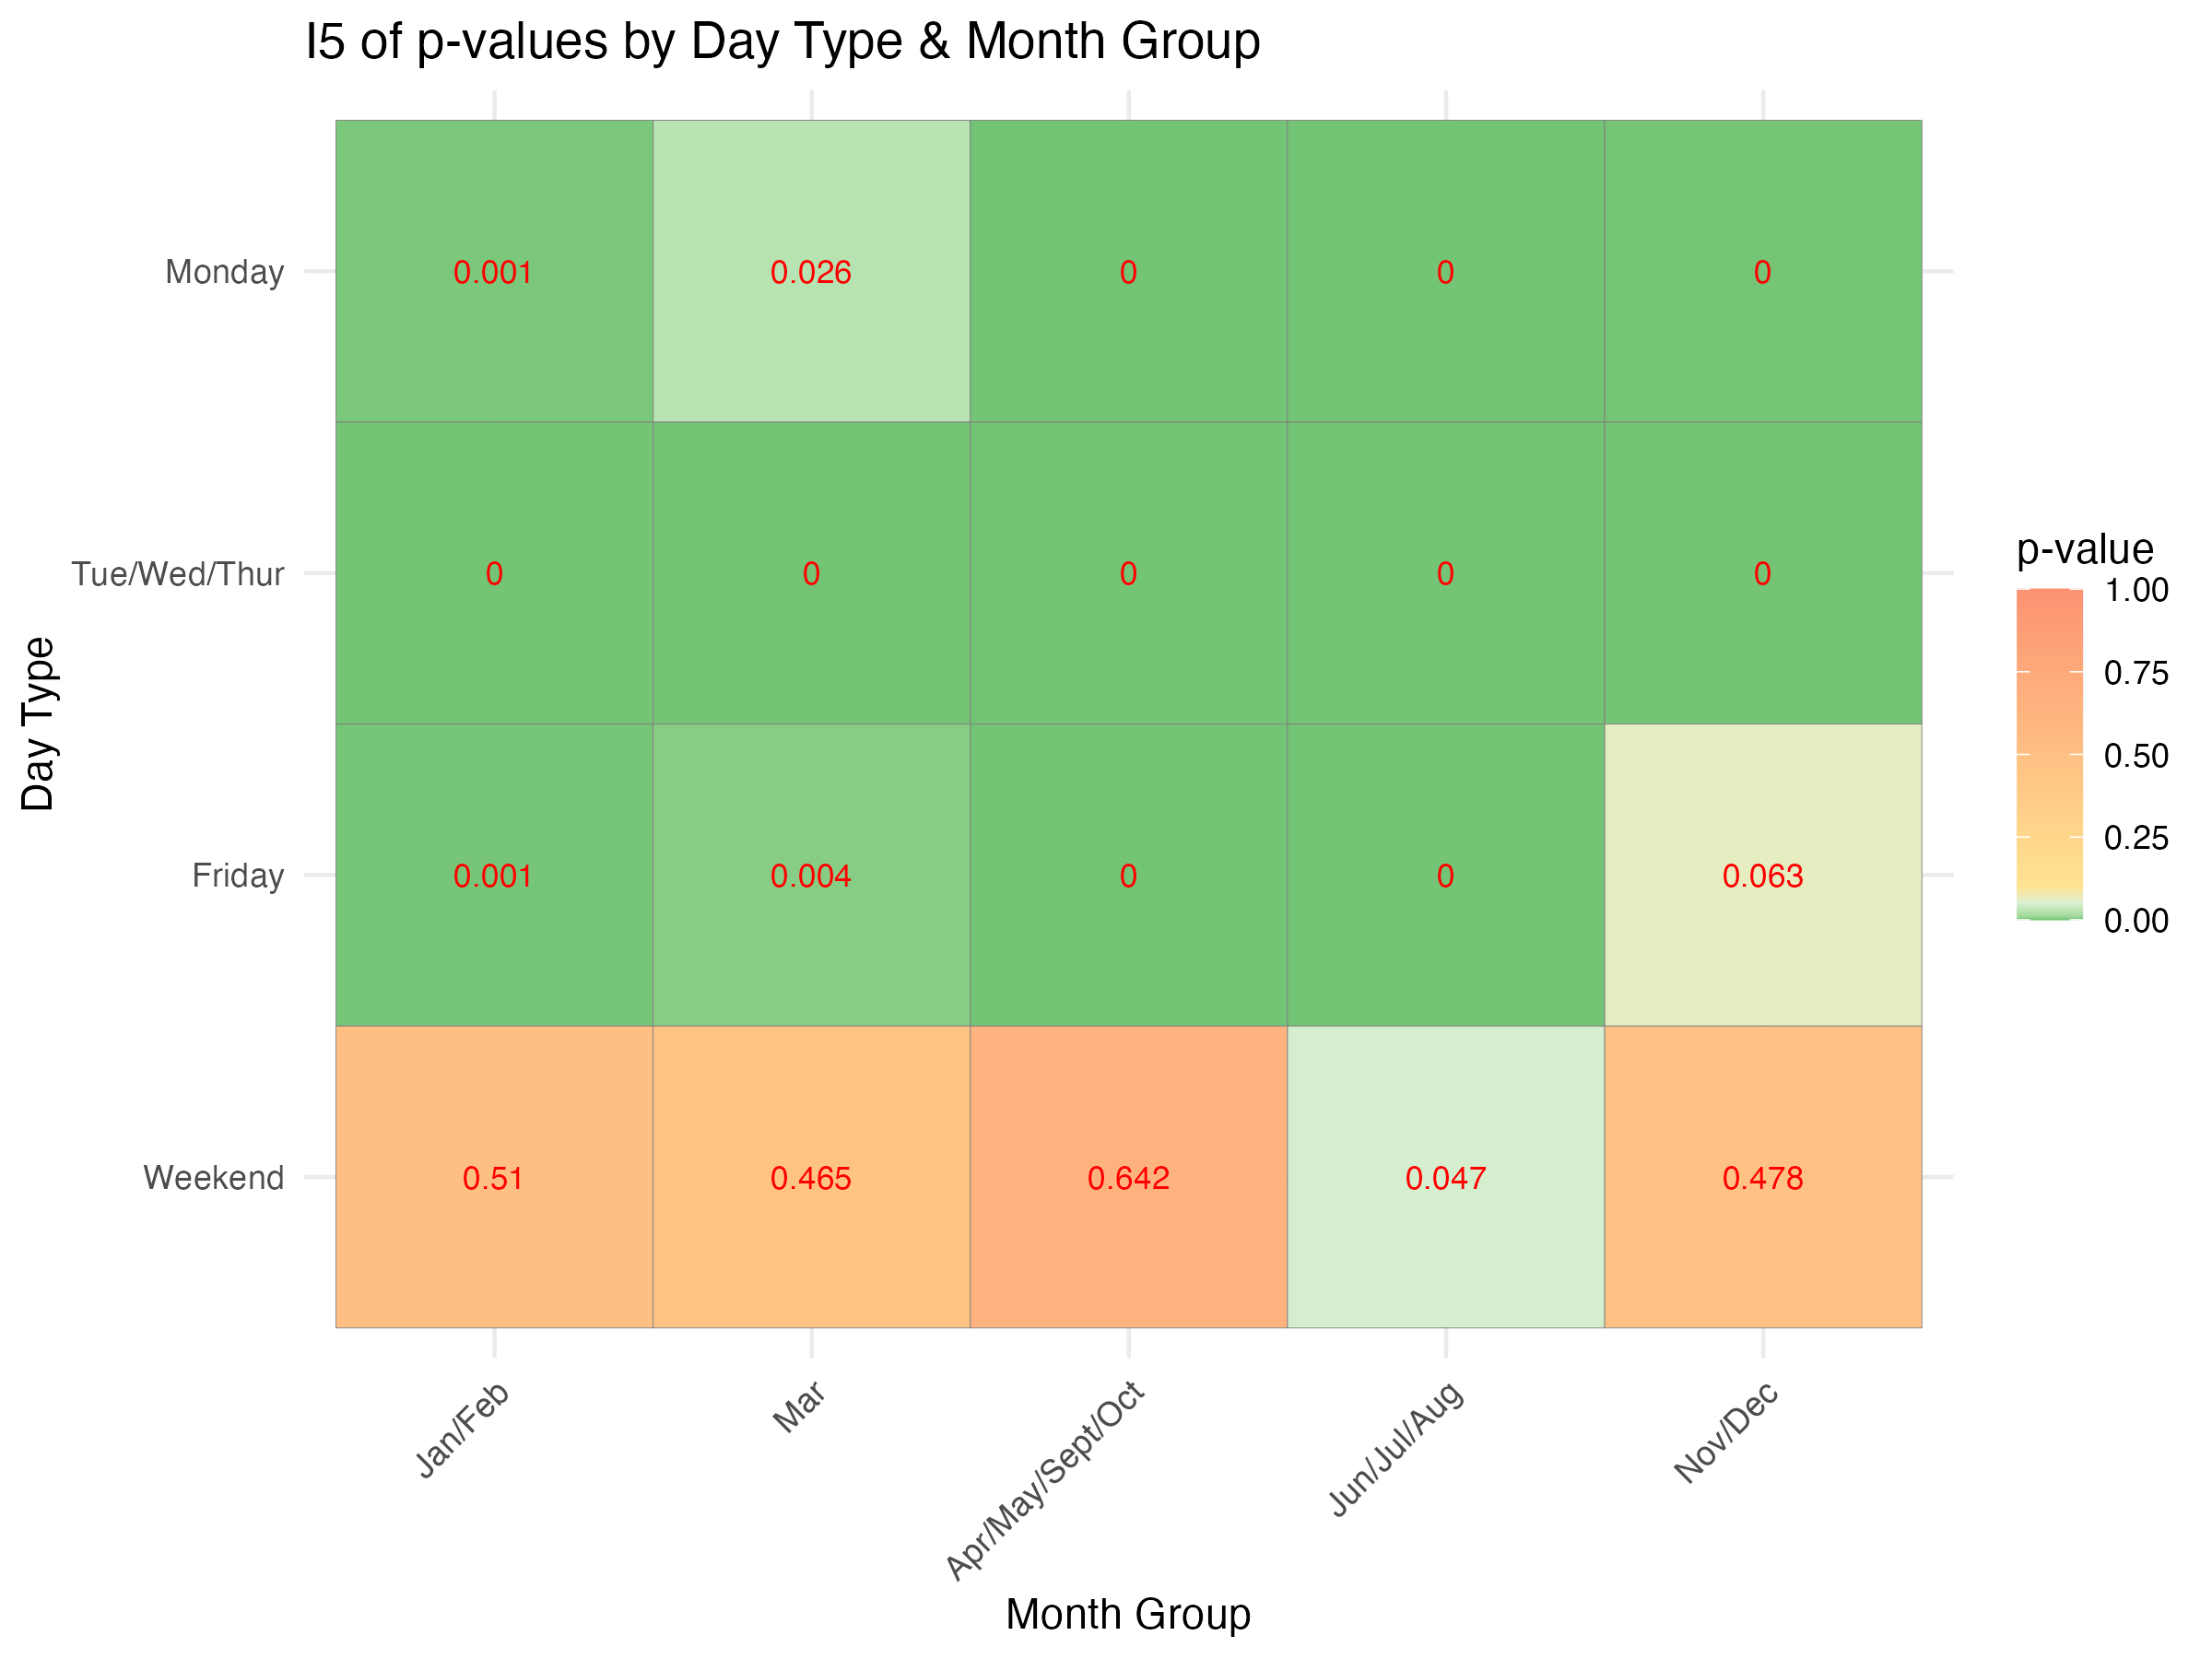
\includegraphics[width=0.75\textwidth]{ATR26004_Plots/pvalues_A04.png}
    \label{fig:i5_pvalues}
\end{figure}

\section{GAM Figures} \label{sec:gam_figs}

\begin{figure}[H]
	\centering
	\begin{subfigure}[b]{0.45\textwidth}
		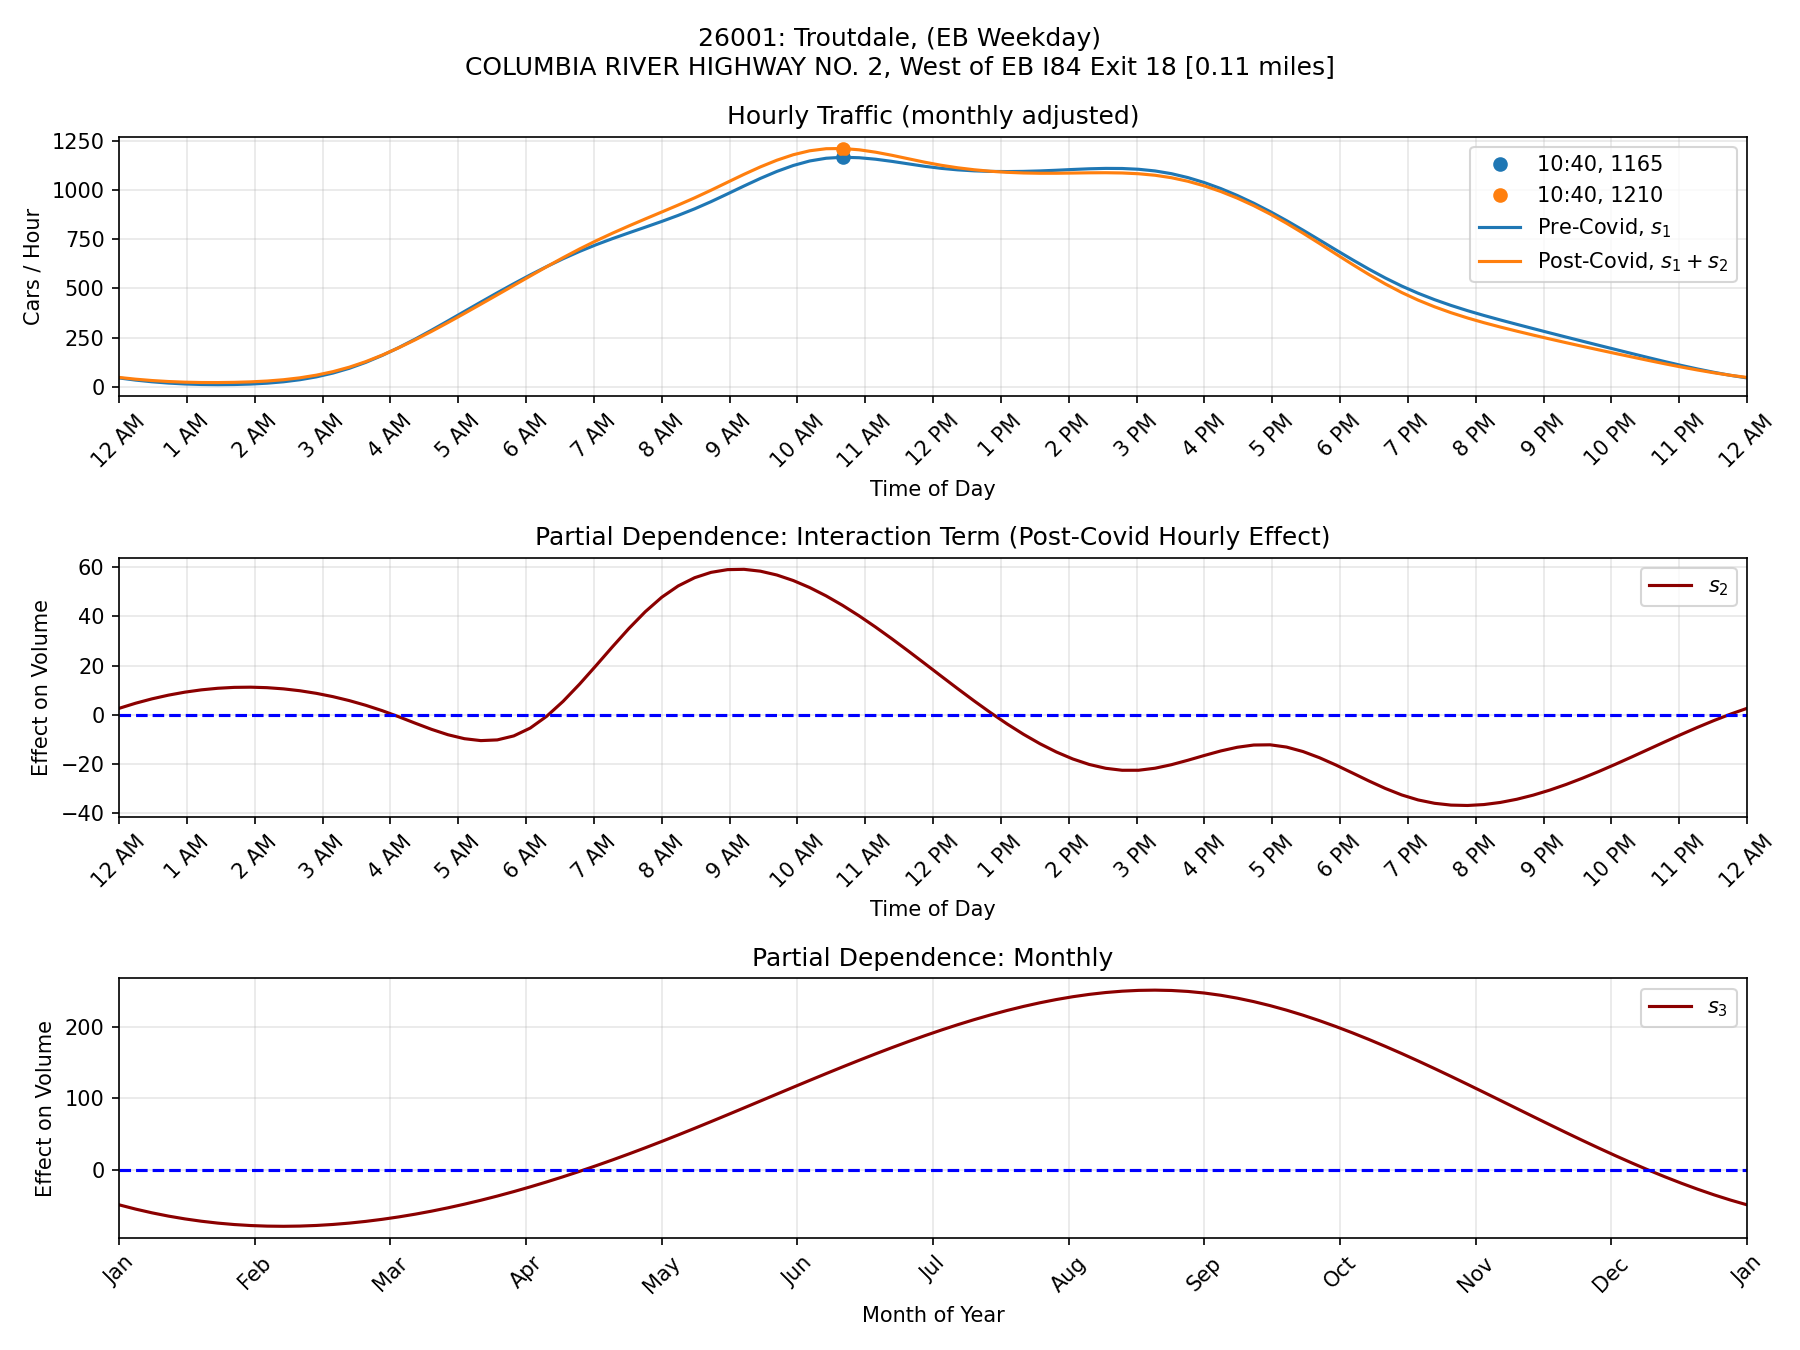
\includegraphics[width=\textwidth]{26001_Troutdale_EB_Weekday_gam.png}
	\end{subfigure}
	\hfill
	\begin{subfigure}[b]{0.45\textwidth}
		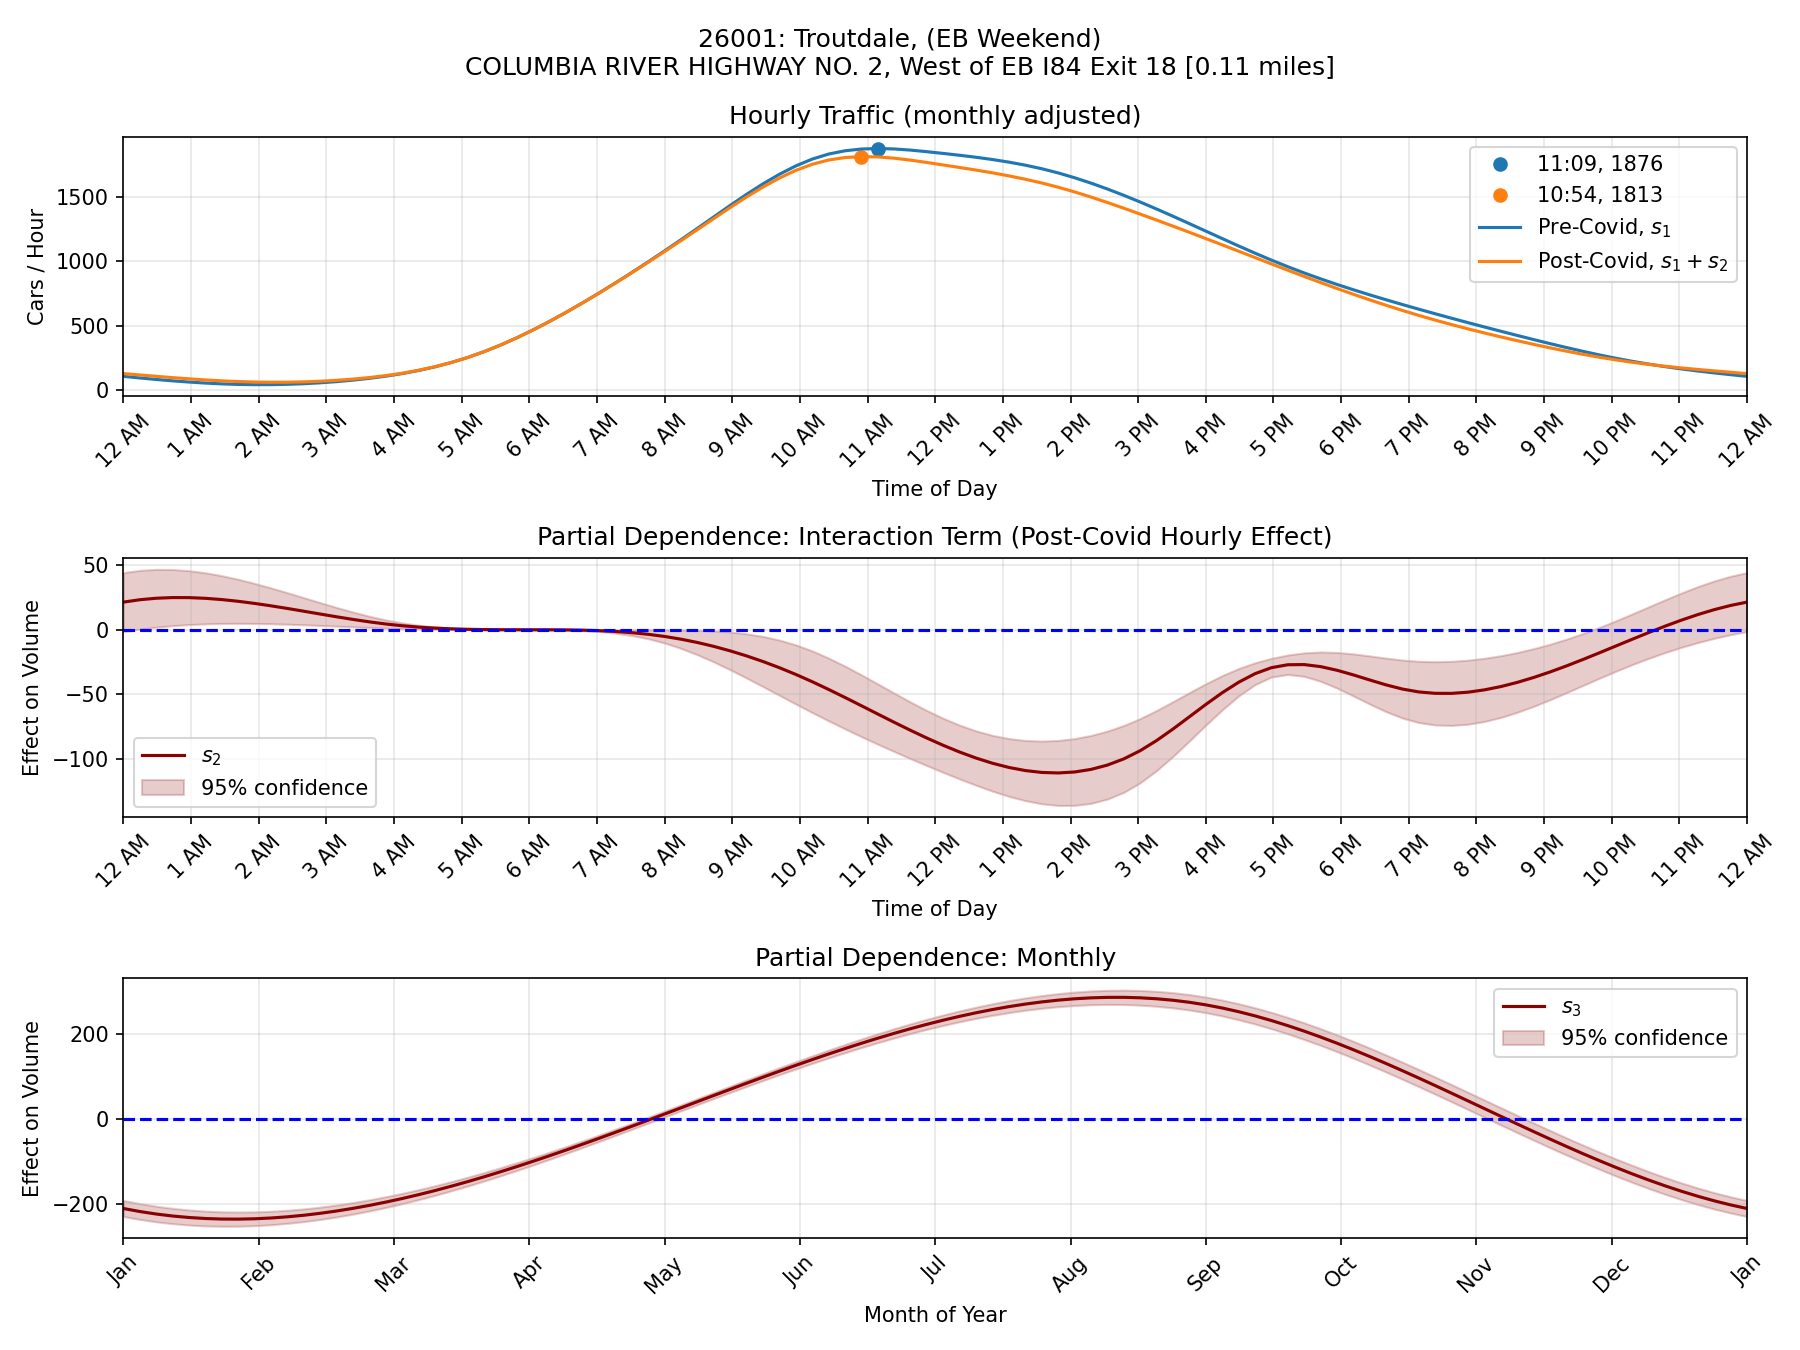
\includegraphics[width=\textwidth]{26001_Troutdale_EB_Weekend_gam.png}
	\end{subfigure}

	\begin{subfigure}[b]{0.45\textwidth}
		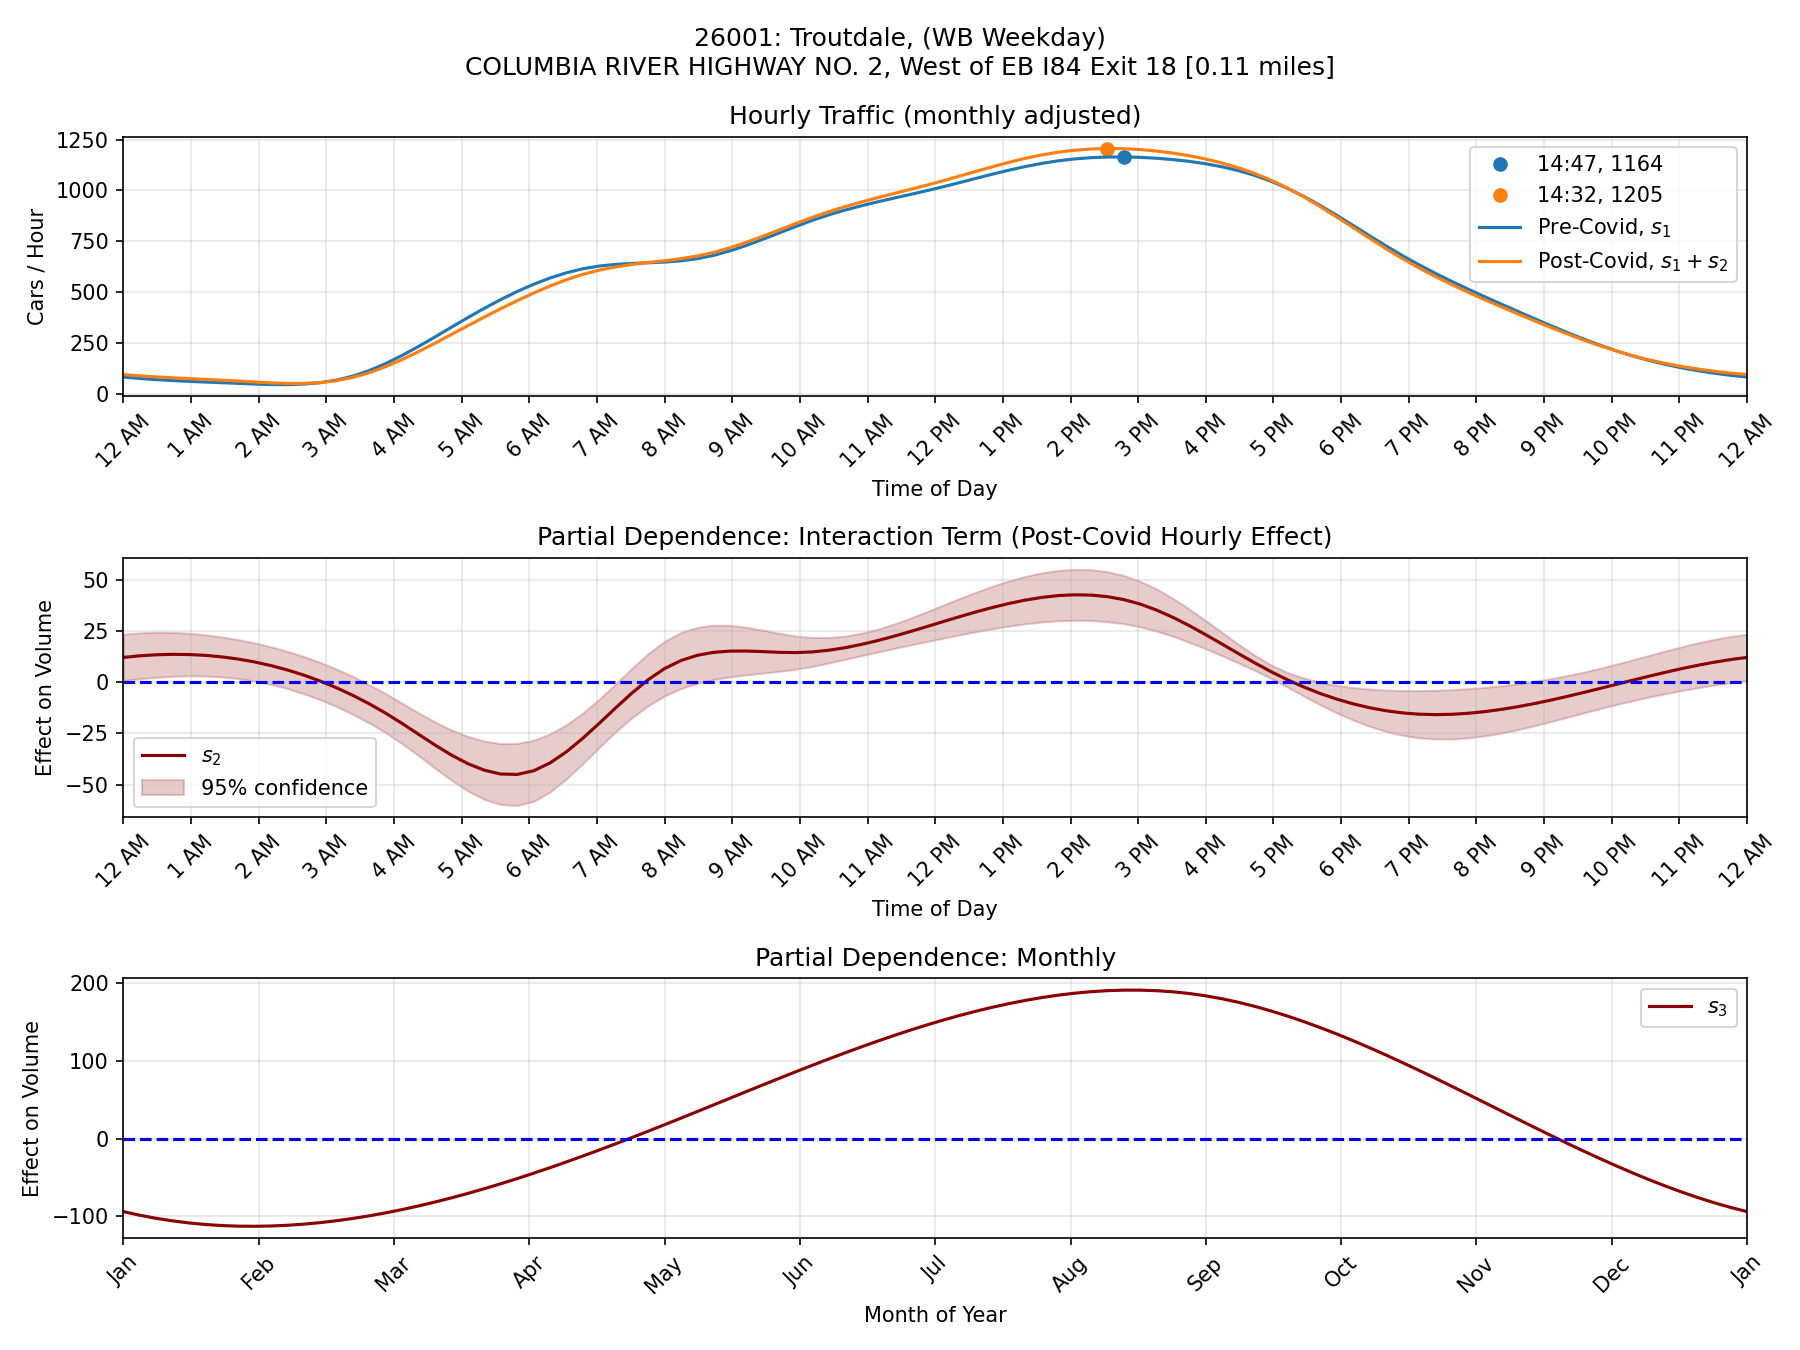
\includegraphics[width=\textwidth]{26001_Troutdale_WB_Weekday_gam.png}
	\end{subfigure}
	\hfill
	\begin{subfigure}[b]{0.45\textwidth}
		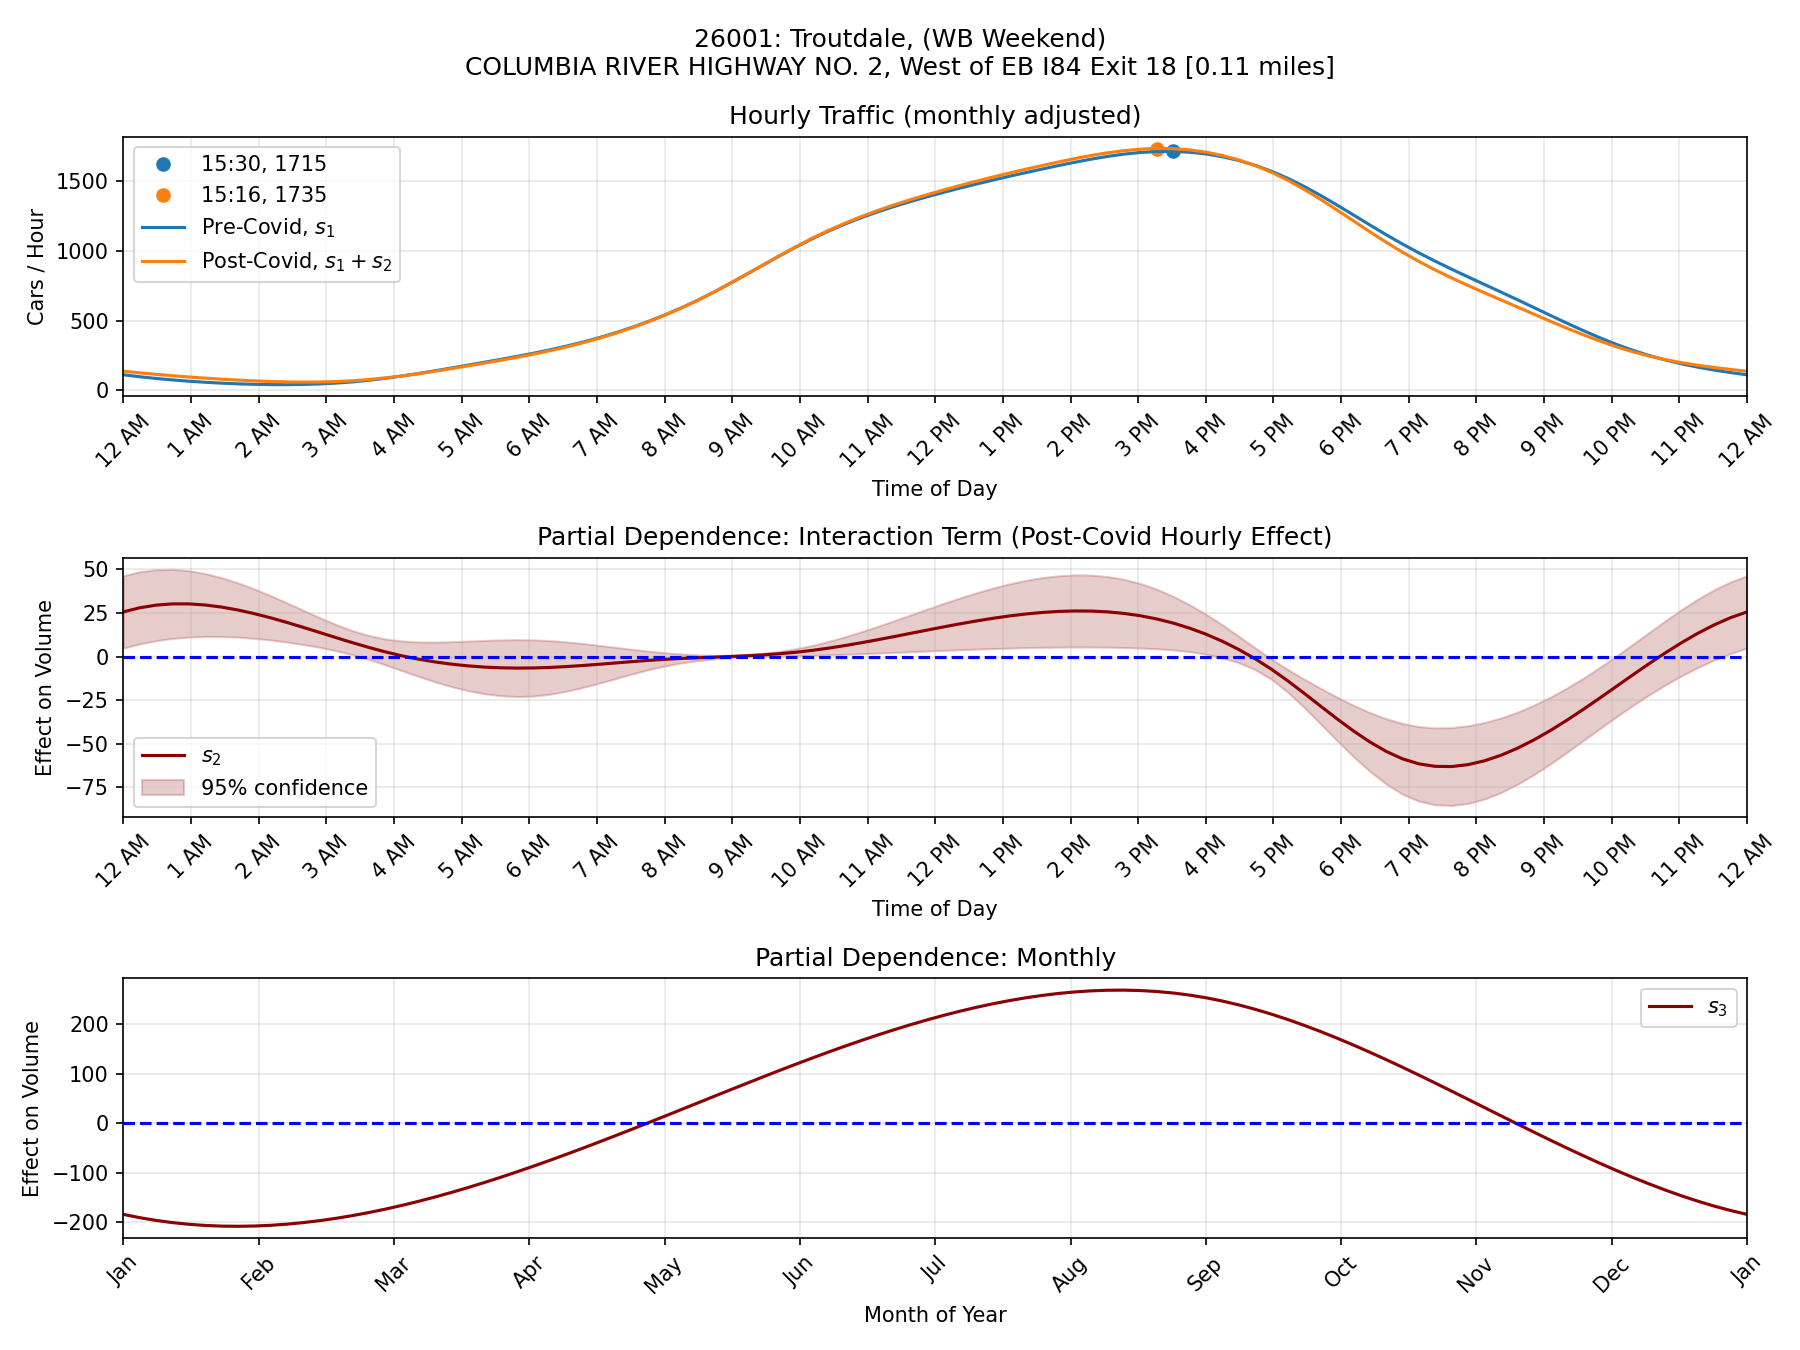
\includegraphics[width=\textwidth]{26001_Troutdale_WB_Weekend_gam.png}
	\end{subfigure}
\end{figure}

\begin{figure}[H]
	\centering
	\begin{subfigure}[b]{0.45\textwidth}
		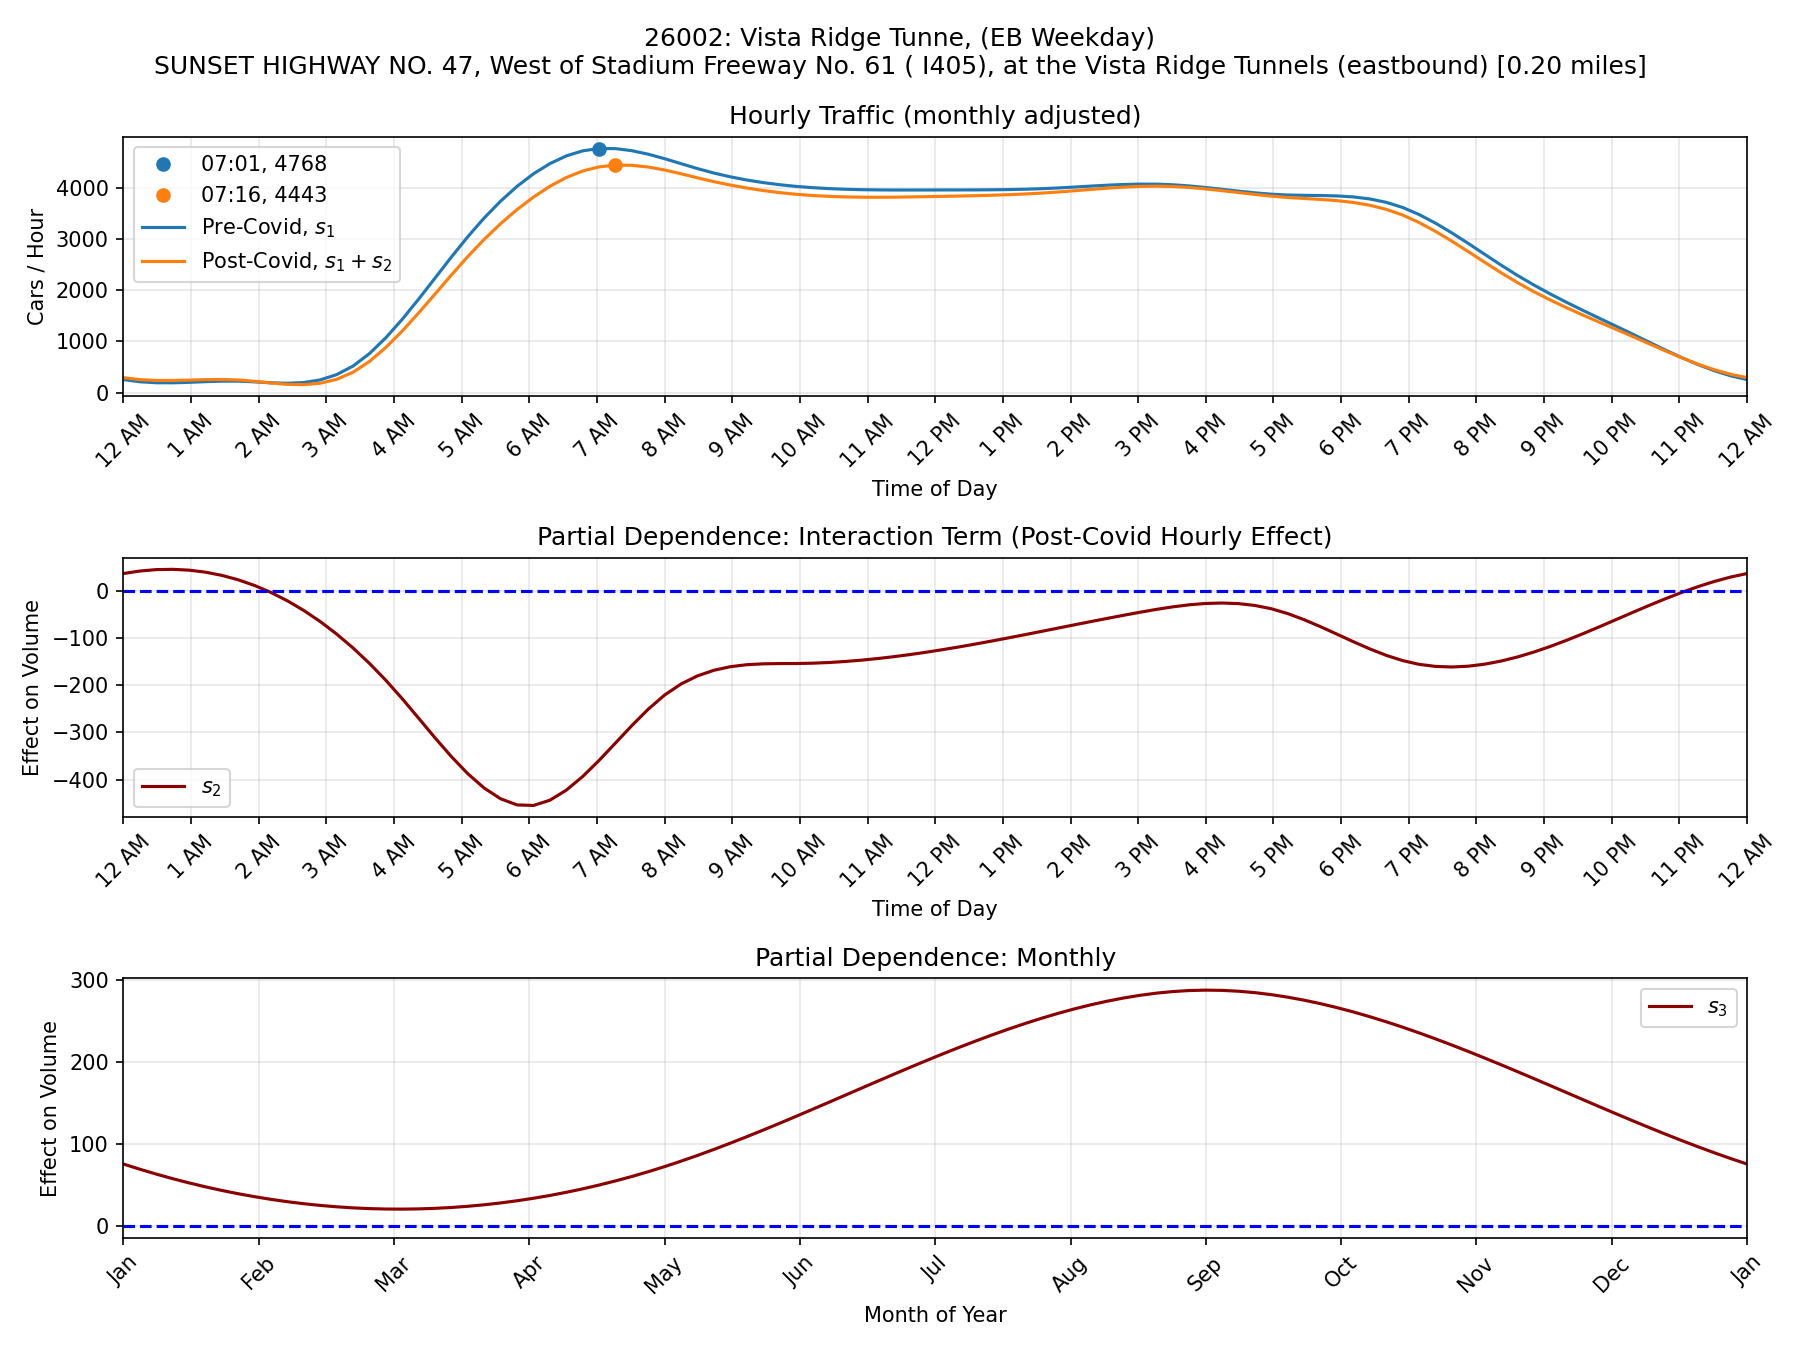
\includegraphics[width=\textwidth]{26002_Vista-Ridge-Tunne_EB_Weekday_gam.png}
	\end{subfigure}
	\hfill
	\begin{subfigure}[b]{0.45\textwidth}
		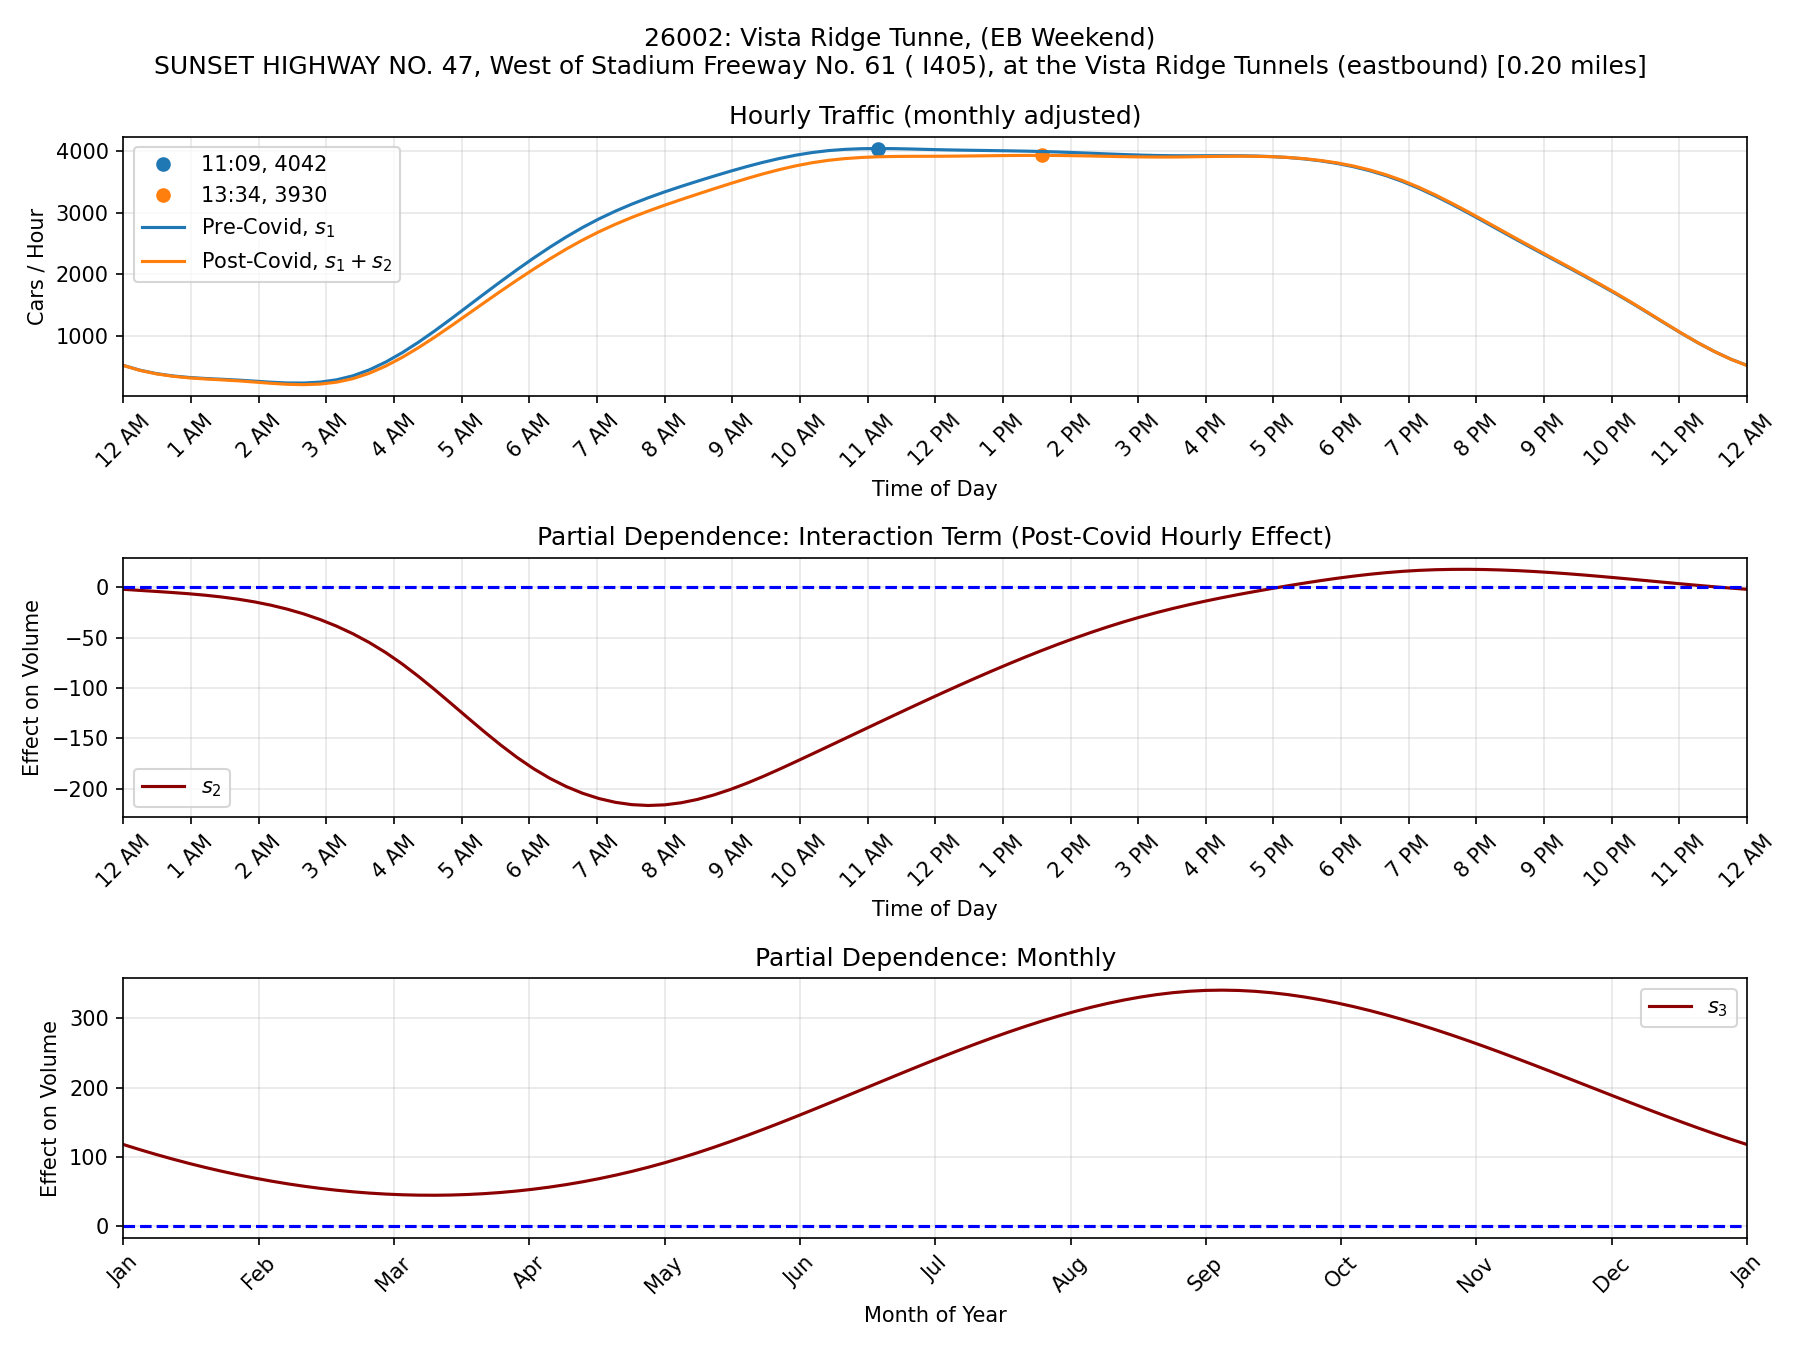
\includegraphics[width=\textwidth]{26002_Vista-Ridge-Tunne_EB_Weekend_gam.png}
	\end{subfigure}

	\begin{subfigure}[b]{0.45\textwidth}
		\includegraphics[width=\textwidth]{26002_Vista-Ridge-Tunne_WB_Weekday_gam.png}
	\end{subfigure}
	\hfill
	\begin{subfigure}[b]{0.45\textwidth}
		\includegraphics[width=\textwidth]{26002_Vista-Ridge-Tunne_WB_Weekend_gam.png}
	\end{subfigure}
\end{figure}

\begin{figure}[H]
	\centering
	\begin{subfigure}[b]{0.45\textwidth}
		\includegraphics[width=\textwidth]{26004_Interstate-Bridge_NB_Weekday_gam.png}
	\end{subfigure}
	\hfill
	\begin{subfigure}[b]{0.45\textwidth}
		\includegraphics[width=\textwidth]{26004_Interstate-Bridge_NB_Weekend_gam.png}
	\end{subfigure}

	\begin{subfigure}[b]{0.45\textwidth}
		\includegraphics[width=\textwidth]{26004_Interstate-Bridge_SB_Weekday_gam.png}
	\end{subfigure}
	\hfill
	\begin{subfigure}[b]{0.45\textwidth}
		\includegraphics[width=\textwidth]{26004_Interstate-Bridge_SB_Weekend_gam.png}
	\end{subfigure}
\end{figure}

\begin{figure}[H]
	\centering
	\begin{subfigure}[b]{0.45\textwidth}
		\includegraphics[width=\textwidth]{26014_Hoyt_EB_Weekday_gam.png}
	\end{subfigure}
	\hfill
	\begin{subfigure}[b]{0.45\textwidth}
		\includegraphics[width=\textwidth]{26014_Hoyt_EB_Weekend_gam.png}
	\end{subfigure}

	\begin{subfigure}[b]{0.45\textwidth}
		\includegraphics[width=\textwidth]{26014_Hoyt_WB_Weekday_gam.png}
	\end{subfigure}
	\hfill
	\begin{subfigure}[b]{0.45\textwidth}
		\includegraphics[width=\textwidth]{26014_Hoyt_WB_Weekend_gam.png}
	\end{subfigure}
\end{figure}

\begin{figure}[H]
	\centering
	\begin{subfigure}[b]{0.45\textwidth}
		\includegraphics[width=\textwidth]{26016_Iowa-Street_NB_Weekday_gam.png}
	\end{subfigure}
	\hfill
	\begin{subfigure}[b]{0.45\textwidth}
		\includegraphics[width=\textwidth]{26016_Iowa-Street_NB_Weekend_gam.png}
	\end{subfigure}

	\begin{subfigure}[b]{0.45\textwidth}
		\includegraphics[width=\textwidth]{26016_Iowa-Street_SB_Weekday_gam.png}
	\end{subfigure}
	\hfill
	\begin{subfigure}[b]{0.45\textwidth}
		\includegraphics[width=\textwidth]{26016_Iowa-Street_SB_Weekend_gam.png}
	\end{subfigure}
\end{figure}

\begin{figure}[H]
	\centering
	\begin{subfigure}[b]{0.45\textwidth}
		\includegraphics[width=\textwidth]{26022_Lents_NB_Weekday_gam.png}
	\end{subfigure}
	\hfill
	\begin{subfigure}[b]{0.45\textwidth}
		\includegraphics[width=\textwidth]{26022_Lents_NB_Weekend_gam.png}
	\end{subfigure}

	\begin{subfigure}[b]{0.45\textwidth}
		\includegraphics[width=\textwidth]{26022_Lents_SB_Weekday_gam.png}
	\end{subfigure}
	\hfill
	\begin{subfigure}[b]{0.45\textwidth}
		\includegraphics[width=\textwidth]{26022_Lents_SB_Weekend_gam.png}
	\end{subfigure}
\end{figure}

\begin{figure}[H]
	\centering
	\begin{subfigure}[b]{0.45\textwidth}
		\includegraphics[width=\textwidth]{26024_Glenn-Jackson-Bridge_NB_Weekday_gam.png}
	\end{subfigure}
	\hfill
	\begin{subfigure}[b]{0.45\textwidth}
		\includegraphics[width=\textwidth]{26024_Glenn-Jackson-Bridge_NB_Weekend_gam.png}
	\end{subfigure}

	\begin{subfigure}[b]{0.45\textwidth}
		\includegraphics[width=\textwidth]{26024_Glenn-Jackson-Bridge_SB_Weekday_gam.png}
	\end{subfigure}
	\hfill
	\begin{subfigure}[b]{0.45\textwidth}
		\includegraphics[width=\textwidth]{26024_Glenn-Jackson-Bridge_SB_Weekend_gam.png}
	\end{subfigure}
\end{figure}

\begin{figure}[H]
	\centering
	\begin{subfigure}[b]{0.45\textwidth}
		\includegraphics[width=\textwidth]{26028_Fairview_EB_Weekday_gam.png}
	\end{subfigure}
	\hfill
	\begin{subfigure}[b]{0.45\textwidth}
		\includegraphics[width=\textwidth]{26028_Fairview_EB_Weekend_gam.png}
	\end{subfigure}

	\begin{subfigure}[b]{0.45\textwidth}
		\includegraphics[width=\textwidth]{26028_Fairview_WB_Weekday_gam.png}
	\end{subfigure}
	\hfill
	\begin{subfigure}[b]{0.45\textwidth}
		\includegraphics[width=\textwidth]{26028_Fairview_WB_Weekend_gam.png}
	\end{subfigure}
\end{figure}

\begin{figure}[H]
	\centering
	\begin{subfigure}[b]{0.45\textwidth}
		\includegraphics[width=\textwidth]{3011_Wilsonville_NB_Weekday_gam.png}
	\end{subfigure}
	\hfill
	\begin{subfigure}[b]{0.45\textwidth}
		\includegraphics[width=\textwidth]{3011_Wilsonville_NB_Weekend_gam.png}
	\end{subfigure}

	\begin{subfigure}[b]{0.45\textwidth}
		\includegraphics[width=\textwidth]{3011_Wilsonville_SB_Weekday_gam.png}
	\end{subfigure}
	\hfill
	\begin{subfigure}[b]{0.45\textwidth}
		\includegraphics[width=\textwidth]{3011_Wilsonville_SB_Weekend_gam.png}
	\end{subfigure}
\end{figure}

\begin{figure}[H]
	\centering
	\begin{subfigure}[b]{0.45\textwidth}
		\includegraphics[width=\textwidth]{3016_Stafford_NB_Weekday_gam.png}
	\end{subfigure}
	\hfill
	\begin{subfigure}[b]{0.45\textwidth}
		\includegraphics[width=\textwidth]{3016_Stafford_NB_Weekend_gam.png}
	\end{subfigure}

	\begin{subfigure}[b]{0.45\textwidth}
		\includegraphics[width=\textwidth]{3016_Stafford_SB_Weekday_gam.png}
	\end{subfigure}
	\hfill
	\begin{subfigure}[b]{0.45\textwidth}
		\includegraphics[width=\textwidth]{3016_Stafford_SB_Weekend_gam.png}
	\end{subfigure}
\end{figure}

\begin{figure}[H]
	\centering
	\begin{subfigure}[b]{0.45\textwidth}
		\includegraphics[width=\textwidth]{34007_North-Plains_EB_Weekday_gam.png}
	\end{subfigure}
	\hfill
	\begin{subfigure}[b]{0.45\textwidth}
		\includegraphics[width=\textwidth]{34007_North-Plains_EB_Weekend_gam.png}
	\end{subfigure}

	\begin{subfigure}[b]{0.45\textwidth}
		\includegraphics[width=\textwidth]{34007_North-Plains_WB_Weekday_gam.png}
	\end{subfigure}
	\hfill
	\begin{subfigure}[b]{0.45\textwidth}
		\includegraphics[width=\textwidth]{34007_North-Plains_WB_Weekend_gam.png}
	\end{subfigure}
\end{figure}

\begin{figure}[H]
	\centering
	\begin{subfigure}[b]{0.45\textwidth}
		\includegraphics[width=\textwidth]{34010_Beaverton-Bethany_EB_Weekday_gam.png}
	\end{subfigure}
	\hfill
	\begin{subfigure}[b]{0.45\textwidth}
		\includegraphics[width=\textwidth]{34010_Beaverton-Bethany_EB_Weekend_gam.png}
	\end{subfigure}

	\begin{subfigure}[b]{0.45\textwidth}
		\includegraphics[width=\textwidth]{34010_Beaverton-Bethany_WB_Weekday_gam.png}
	\end{subfigure}
	\hfill
	\begin{subfigure}[b]{0.45\textwidth}
		\includegraphics[width=\textwidth]{34010_Beaverton-Bethany_WB_Weekend_gam.png}
	\end{subfigure}
\end{figure}


\section{Data Availability}

\begin{figure}[H] 
    \centering
    \includegraphics[width=0.9\textwidth]{missing_data.png}
    \caption{Red indicates missing data, opacity indicates how much of that week is missing. This doesn't account for ``0'' data which is technically missing and misrepresented.}
    \label{fig:data_availability}
\end{figure}

\section{Data Issues Deep Dive by Locations} \label{app:data_issues}

\begin{figure}[H] 
    \centering
    \includegraphics[width=0.9\textwidth]{dst_issue.png}
    \caption{An example of when the data seems to be shifted by exactly an hour indicating issues with how DST was handled. Interestingly, the date ranges don't match exactly with when the time changes happen.}
    \label{fig:dst_example}
\end{figure}

These plots provide a visual for similar data presented in table \ref{tab:medians} but includes every year available in the dataset with quantile shading. Each line is the periodic cubic spline interpolation of the hourly medians/quantiles for each (location, direction, weekday/weekend) tuple. Some strange data issues become apparent in these plots, but they are almost entirely only in years we aren't concerned with in this analysis.
\begin{figure}[htbp]
	\centering
	\begin{subfigure}{0.45\textwidth}
		\includegraphics[width=\textwidth]{26001_Troutdale_EB_Weekday.png}
	\end{subfigure}
	\hfill
	\begin{subfigure}{0.45\textwidth}
		\includegraphics[width=\textwidth]{26001_Troutdale_EB_Weekend.png}
	\end{subfigure}

	\begin{subfigure}{0.45\textwidth}
		\includegraphics[width=\textwidth]{26001_Troutdale_WB_Weekday.png}
	\end{subfigure}
	\hfill
	\begin{subfigure}{0.45\textwidth}
		\includegraphics[width=\textwidth]{26001_Troutdale_WB_Weekend.png}
	\end{subfigure}
\end{figure}

\begin{figure}[htbp]
	\centering
	\begin{subfigure}{0.45\textwidth}
		\includegraphics[width=\textwidth]{26002_Vista-Ridge-Tunne_EB_Weekday.png}
	\end{subfigure}
	\hfill
	\begin{subfigure}{0.45\textwidth}
		\includegraphics[width=\textwidth]{26002_Vista-Ridge-Tunne_EB_Weekend.png}
	\end{subfigure}

	\begin{subfigure}{0.45\textwidth}
		\includegraphics[width=\textwidth]{26002_Vista-Ridge-Tunne_WB_Weekday.png}
	\end{subfigure}
	\hfill
	\begin{subfigure}{0.45\textwidth}
		\includegraphics[width=\textwidth]{26002_Vista-Ridge-Tunne_WB_Weekend.png}
	\end{subfigure}
\end{figure}

\begin{figure}[htbp]
	\centering
	\begin{subfigure}{0.45\textwidth}
		\includegraphics[width=\textwidth]{26004_Interstate-Bridge_NB_Weekday.png}
	\end{subfigure}
	\hfill
	\begin{subfigure}{0.45\textwidth}
		\includegraphics[width=\textwidth]{26004_Interstate-Bridge_NB_Weekend.png}
	\end{subfigure}

	\begin{subfigure}{0.45\textwidth}
		\includegraphics[width=\textwidth]{26004_Interstate-Bridge_SB_Weekday.png}
	\end{subfigure}
	\hfill
	\begin{subfigure}{0.45\textwidth}
		\includegraphics[width=\textwidth]{26004_Interstate-Bridge_SB_Weekend.png}
	\end{subfigure}
\end{figure}

\begin{figure}[htbp]
	\centering
	\begin{subfigure}{0.45\textwidth}
		\includegraphics[width=\textwidth]{26014_Hoyt_EB_Weekday.png}
	\end{subfigure}
	\hfill
	\begin{subfigure}{0.45\textwidth}
		\includegraphics[width=\textwidth]{26014_Hoyt_EB_Weekend.png}
	\end{subfigure}

	\begin{subfigure}{0.45\textwidth}
		\includegraphics[width=\textwidth]{26014_Hoyt_WB_Weekday.png}
	\end{subfigure}
	\hfill
	\begin{subfigure}{0.45\textwidth}
		\includegraphics[width=\textwidth]{26014_Hoyt_WB_Weekend.png}
	\end{subfigure}
\end{figure}

\begin{figure}[htbp]
	\centering
	\begin{subfigure}{0.45\textwidth}
		\includegraphics[width=\textwidth]{26016_Iowa-Street_NB_Weekday.png}
	\end{subfigure}
	\hfill
	\begin{subfigure}{0.45\textwidth}
		\includegraphics[width=\textwidth]{26016_Iowa-Street_NB_Weekend.png}
	\end{subfigure}

	\begin{subfigure}{0.45\textwidth}
		\includegraphics[width=\textwidth]{26016_Iowa-Street_SB_Weekday.png}
	\end{subfigure}
	\hfill
	\begin{subfigure}{0.45\textwidth}
		\includegraphics[width=\textwidth]{26016_Iowa-Street_SB_Weekend.png}
	\end{subfigure}
\end{figure}

\begin{figure}[htbp]
	\centering
	\begin{subfigure}{0.45\textwidth}
		\includegraphics[width=\textwidth]{26022_Lents_NB_Weekday.png}
	\end{subfigure}
	\hfill
	\begin{subfigure}{0.45\textwidth}
		\includegraphics[width=\textwidth]{26022_Lents_NB_Weekend.png}
	\end{subfigure}

	\begin{subfigure}{0.45\textwidth}
		\includegraphics[width=\textwidth]{26022_Lents_SB_Weekday.png}
	\end{subfigure}
	\hfill
	\begin{subfigure}{0.45\textwidth}
		\includegraphics[width=\textwidth]{26022_Lents_SB_Weekend.png}
	\end{subfigure}
\end{figure}

\begin{figure}[htbp]
	\centering
	\begin{subfigure}{0.45\textwidth}
		\includegraphics[width=\textwidth]{26024_Glenn-Jackson-Bridge_NB_Weekday.png}
	\end{subfigure}
	\hfill
	\begin{subfigure}{0.45\textwidth}
		\includegraphics[width=\textwidth]{26024_Glenn-Jackson-Bridge_NB_Weekend.png}
	\end{subfigure}

	\begin{subfigure}{0.45\textwidth}
		\includegraphics[width=\textwidth]{26024_Glenn-Jackson-Bridge_SB_Weekday.png}
	\end{subfigure}
	\hfill
	\begin{subfigure}{0.45\textwidth}
		\includegraphics[width=\textwidth]{26024_Glenn-Jackson-Bridge_SB_Weekend.png}
	\end{subfigure}
\end{figure}

\begin{figure}[htbp]
	\centering
	\begin{subfigure}{0.45\textwidth}
		\includegraphics[width=\textwidth]{26028_Fairview_EB_Weekday.png}
	\end{subfigure}
	\hfill
	\begin{subfigure}{0.45\textwidth}
		\includegraphics[width=\textwidth]{26028_Fairview_EB_Weekend.png}
	\end{subfigure}

	\begin{subfigure}{0.45\textwidth}
		\includegraphics[width=\textwidth]{26028_Fairview_WB_Weekday.png}
	\end{subfigure}
	\hfill
	\begin{subfigure}{0.45\textwidth}
		\includegraphics[width=\textwidth]{26028_Fairview_WB_Weekend.png}
	\end{subfigure}
\end{figure}

\begin{figure}[htbp]
	\centering
	\begin{subfigure}{0.45\textwidth}
		\includegraphics[width=\textwidth]{3011_Wilsonville_NB_Weekday.png}
	\end{subfigure}
	\hfill
	\begin{subfigure}{0.45\textwidth}
		\includegraphics[width=\textwidth]{3011_Wilsonville_NB_Weekend.png}
	\end{subfigure}

	\begin{subfigure}{0.45\textwidth}
		\includegraphics[width=\textwidth]{3011_Wilsonville_SB_Weekday.png}
	\end{subfigure}
	\hfill
	\begin{subfigure}{0.45\textwidth}
		\includegraphics[width=\textwidth]{3011_Wilsonville_SB_Weekend.png}
	\end{subfigure}
\end{figure}

\begin{figure}[htbp]
	\centering
	\begin{subfigure}{0.45\textwidth}
		\includegraphics[width=\textwidth]{3016_Stafford_NB_Weekday.png}
	\end{subfigure}
	\hfill
	\begin{subfigure}{0.45\textwidth}
		\includegraphics[width=\textwidth]{3016_Stafford_NB_Weekend.png}
	\end{subfigure}

	\begin{subfigure}{0.45\textwidth}
		\includegraphics[width=\textwidth]{3016_Stafford_SB_Weekday.png}
	\end{subfigure}
	\hfill
	\begin{subfigure}{0.45\textwidth}
		\includegraphics[width=\textwidth]{3016_Stafford_SB_Weekend.png}
	\end{subfigure}
\end{figure}

\begin{figure}[htbp]
	\centering
	\begin{subfigure}{0.45\textwidth}
		\includegraphics[width=\textwidth]{34007_North-Plains_EB_Weekday.png}
	\end{subfigure}
	\hfill
	\begin{subfigure}{0.45\textwidth}
		\includegraphics[width=\textwidth]{34007_North-Plains_EB_Weekend.png}
	\end{subfigure}

	\begin{subfigure}{0.45\textwidth}
		\includegraphics[width=\textwidth]{34007_North-Plains_WB_Weekday.png}
	\end{subfigure}
	\hfill
	\begin{subfigure}{0.45\textwidth}
		\includegraphics[width=\textwidth]{34007_North-Plains_WB_Weekend.png}
	\end{subfigure}
\end{figure}

\begin{figure}[htbp]
	\centering
	\begin{subfigure}{0.45\textwidth}
		\includegraphics[width=\textwidth]{34010_Beaverton-Bethany_EB_Weekday.png}
	\end{subfigure}
	\hfill
	\begin{subfigure}{0.45\textwidth}
		\includegraphics[width=\textwidth]{34010_Beaverton-Bethany_EB_Weekend.png}
	\end{subfigure}

	\begin{subfigure}{0.45\textwidth}
		\includegraphics[width=\textwidth]{34010_Beaverton-Bethany_WB_Weekday.png}
	\end{subfigure}
	\hfill
	\begin{subfigure}{0.45\textwidth}
		\includegraphics[width=\textwidth]{34010_Beaverton-Bethany_WB_Weekend.png}
	\end{subfigure}
\end{figure}

\end{document}
